
\documentclass[12pt]{report}
\usepackage{textcomp}

\addtolength{\hoffset}{-2.25cm}
\addtolength{\textwidth}{4.5cm}
\addtolength{\voffset}{-2.5cm}
\addtolength{\textheight}{5cm}
\setlength{\parskip}{0pt}
\setlength{\parindent}{15pt}

\usepackage{graphicx}
\graphicspath{ {./images/} }

\usepackage{amsthm}
\usepackage{amsmath}
\usepackage{amssymb}
\usepackage{dutchcal}

\newcommand{\be}{\beta}
\newcommand{\ga}{\gamma}

\usepackage[colorlinks = true, linkcolor = black, citecolor = black, final]{hyperref}
\hypersetup{
    colorlinks,
    citecolor=black,
    filecolor=black,
    linkcolor=black,
    urlcolor=black
}

\usepackage{graphicx}
\usepackage{multicol}
\usepackage{marvosym}
\usepackage{wasysym}

\usepackage{outlines}
\usepackage[utf8]{inputenc}
\usepackage[english]{babel}

\usepackage{enumitem,amssymb}

\newcommand{\pr}[1]{\left(#1\right)}
\newcommand{\cross}{\times}
\newcommand{\grad}{\nabla}

\usepackage{pgfplots}
\pgfplotsset{compat=1.16}
\usepackage{circuitikz}
\usepackage{tikz}
\usetikzlibrary{patterns}
\usetikzlibrary{arrows.meta}

\usepackage{mdframed}
\usepackage{pbox}
\usepackage{array}
\usepackage{makecell}
\usepackage{booktabs}
\setlength{\heavyrulewidth}{1pt}
\setlength{\abovetopsep}{4pt}


\setlength{\parindent}{0in}
\usepackage{changepage}

\pagestyle{plain}

\definecolor{codegreen}{rgb}{0,0.6,0}
\definecolor{codegray}{rgb}{0.5,0.5,0.5}
\definecolor{codepurple}{rgb}{0.58,0,0.82}
\definecolor{backcolour}{rgb}{0.95,0.95,0.92}
\definecolor{backcolour2}{rgb}{0.44,0.63,0.99}

\definecolor{dkgreen}{rgb}{0,0.6,0}
\definecolor{gray}{rgb}{0.5,0.5,0.5}
\definecolor{mauve}{rgb}{0.58,0,0.82}

\usepackage{listings}
\lstset{
    language=Verilog,
    breakatwhitespace=false,         
    breaklines=true,                 
    captionpos=b,                    
    keepspaces=true,                 
    numbers=left,                    
    numbersep=5pt,                  
    showspaces=false,                
    showstringspaces=false,
    showtabs=false       
    columns=flexible,
    basicstyle={\small\ttfamily},
    numberstyle=\tiny\color{gray},
    keywordstyle=\color{blue},
    commentstyle=\color{dkgreen},
     % stringstyle=\color{mauve},
    stringstyle=\color{orange},
    backgroundcolor=\color{backcolour},
    tabsize=4  
}

\lstnewenvironment{CPP}
  {\lstset{language=C,basicstyle=\ttfamily\small,frame=none}}
  {}

\usepackage{lmodern}
\usepackage{afterpage}
\usepackage{adjustbox}
\usepackage{helvet}

\counterwithout{footnote}{chapter} % makes footnotes count over document rather than by chapter

%%%%%%%%%%%%%%%% These commands are taken from Professor Ashmanskas!
\newcommand{\ohm}{\Omega}
\newcommand{\kohm}{{\rm k}\Omega}
\newcommand{\Mohm}{{\rm M}\Omega}
\newcommand{\dif}{{\rm d}}
\newcommand{\kgmps}{{\rm kg\cdot m/s}}
\newcommand{\degC}{{}^\circ{\rm C}}
\newcommand{\degF}{{}^\circ{\rm F}}
\newcommand{\K}{{\rm K}}
\newcommand{\liter}{{\rm L}}
\newcommand{\mL}{{\rm mL}}
\newcommand{\atm}{{\rm atm}}
\newcommand{\mol}{{\rm mol}}
\newcommand{\Cal}{{\rm Cal}}
\newcommand{\W}{{\rm W}}
\newcommand{\kW}{{\rm kW}}
\newcommand{\dB}{{\rm dB}}
\newcommand{\amu}{{\rm u}}
\newcommand{\Pa}{{\rm Pa}}
\newcommand{\J}{{\rm J}}
\newcommand{\N}{{\rm N}}
\newcommand{\pC}{{\rm pC}}
\newcommand{\C}{{\rm C}}
\newcommand{\T}{{\rm T}}
\newcommand{\eV}{{\rm eV}}
\newcommand{\V}{{\rm V}}
\newcommand{\mV}{{\rm mV}}
\newcommand{\Vpp}{{ V}_{ pp}}
\newcommand{\mVpp}{{\rm mV}_{\rm pp}}
\newcommand{\Vac}{{\rm V}_{\rm AC}}
\newcommand{\Vdc}{{\rm V}_{\rm DC}}
\newcommand{\Vbold}{{\bf V}}
\newcommand{\Ibold}{{\bf I}}
\newcommand{\Zbold}{{\bf Z}}
\newcommand{\kV}{{\rm kV}}
\newcommand{\emf}{{\cal E}}
\newcommand{\A}{{\rm A}}
\newcommand{\mA}{{\rm mA}}
\newcommand{\uA}{{\rm \mu A}}
\newcommand{\nA}{{\rm nA}}
\newcommand{\F}{{\rm F}}
\newcommand{\uF}{\mu{\rm F}}
\newcommand{\nF}{{\rm nF}}
\newcommand{\pF}{{\rm pF}}
\newcommand{\mH}{{\rm mH}}
\newcommand{\muH}{{\rm \mu H}}
\newcommand{\uC}{\mu{\rm C}}
\newcommand{\nC}{{\rm nC}}
\newcommand{\MJ}{{\rm MJ}}
\newcommand{\kJ}{{\rm kJ}}
\newcommand{\kg}{{\rm kg}}
\newcommand{\g}{{\rm g}}
\newcommand{\m}{{\rm m}}
\newcommand{\s}{{\rm s}}
\newcommand{\ms}{\rm ms}
\newcommand{\us}{\mu{\rm s}}
\newcommand{\ns}{{\rm ns}}
\newcommand{\cm}{{\rm cm}}
\newcommand{\um}{\mu{\rm m}}
\newcommand{\mm}{{\rm mm}}
\newcommand{\nm}{{\rm nm}}
\newcommand{\km}{{\rm km}}
\newcommand{\G}{{6.67\times10^{-11}~\frac{\N~\m^2}{\kg^2}}}
\newcommand{\mpsps}{\frac{\m}{\s^2}}
\newcommand{\kgmsq}{\kg\cdot\m^2}
\newcommand{\Nm}{\N~\m}      % {\N\cdot\m}
\newcommand{\ihat}{{\hat{i}}}
\newcommand{\jhat}{{\hat{j}}}
\newcommand{\khat}{{\hat{k}}}
\newcommand{\Hz}{{\rm Hz}}
\newcommand{\kHz}{{\rm kHz}}
\newcommand{\MHz}{{\rm MHz}}
\newcommand{\kN}{{\rm kN}}
\newcommand{\red}{\color{red}}
%%%%%%%%%%%%%%%%%%%%%%%%%%

\newcommand{\lst}{\lstinline}
\newcommand{\bs}{\bigskip}
\newcommand{\Vo}{{V}_{out}}
\newcommand{\Vi}{{V}_{in}}
\newcommand{\fdb}{{f}_{3dB}}




%%%%%%%%%%%%%%%%%%%%%%%%%
% Some macros

\newcommand\myNIA[4]{%1: name of this amplifier, %2 start coordinate, %3 R1, %4 R2
\draw 
#2 coordinate(#1-in) to[short] ++(1,0)
node[op amp, noinv input up, anchor=+](#1-OA){\texttt{#1}}
(#1-OA.-) -- ++(0,-1) coordinate(#1-FB)
to[R=#3] ++(0,-2) node[ground]{}
(#1-FB) to[R=#4, *-] (#1-FB -| #1-OA.out) -- (#1-OA.out)
to [short, *-] ++(1,0) coordinate(#1-out)
;
}

\newcommand\myF[2]{
%1: name of this follower, %2 start coordinate
\draw
#2 to ++(2,0.5) coordinate(start)
(start) node[op amp](#1-OA){\texttt{F1}} (opamp) {}

(opamp.+) node[left] {}
to [short, *-] ++(-1,0) coordinate(#1-in)

(opamp.-) node[left] {}
to[short] ++(0,1)

(opamp.out) node[right] {}
to[short] ++(0,1.5)
to[short] ++(-2.4,0) 
(opamp.out) coordinate(#1-out)
;
}

\newcommand\myDividers[4]{
%1: exit of divider 1, %2 exit of divider 2
\draw
#3 coordinate(#4-in)
#1 to [battery, l=9 V] ++(0,2)
to [R, l=1 k$\Omega$] ++(2,0) coordinate(#4-out)
to [R, l=2 k$\Omega$] ++(0,-2) 

(2,2) to [short] #2

#1 to [short, -*] ++(9,0)

#3 to [R, l=1 k$\Omega$] ++(2,0)
to [R, l=2 k$\Omega$] ++(0,-2)
(8,2) to [short, -*] ++(1,0)
;
}



%%%%%%%%%%%%%%%%%%%%%%%%%


\begin{document}

\bigskip
\bigskip
\bigskip
\bigskip
\begin{titlepage}

\pagecolor{black}\afterpage{\nopagecolor}


       \vspace*{1in}
       
\begin{adjustbox}{minipage=10cm,scale={2}{3}}

       \textbf{\fontsize{40}{40}\selectfont \textcolor{white}{BRAIN-\\SPINE-\\MUSCLE}}\newline
       \vspace{-0.2in}
       \textbf{\fontsize{30}{30}\selectfont \textcolor{white}{INTERFACES}}\\

\end{adjustbox}

       \smallskip 

       \vspace{0.5in}

       {\fontfamily{phv}\selectfont \textbf{\Large \textcolor{white}{BY: JACKSON POWELL \\ \small FOR: 
       \textcolor{red}{FUTURE} JACKSON}}} \\
       \begin{flushright}
       \textcolor{white}{\texttt {root@/last$\_$updated:}} \textcolor{red}{\texttt{\today}}
       \end{flushright}

    \vspace{1cm}

\begin{flushright}

        {\fontfamily{phv}\selectfont\textbf{\large \textcolor{white}{Once you know the way broadly, you can see it in all things.\\
        -- The Book of Five Rings by Miyamoto Musashi}}}
    
\end{flushright} 


\vspace{0.5cm}
        
\centerline{\rule{13cm}{0.4pt}}
\tableofcontents
\centerline{\rule{13cm}{0.4pt}}
            
       \vspace{0.8cm}
     


\end{titlepage}

\pagebreak




% {\scshape J. Powell} \hfill {\scshape \large Brain-Spine-Muscle Interfaces} \hfill {\scshape 2023}
 
% \smallskip

% \hrule
% \bigskip
% \normalsize 


\chapter{Prologue}

\subsection{Purpose}
The purpose of this book is to aggregate all of the content and tools I will need in forging the future I desire: building better brain-spine-muscle interfaces. Interestingly, I already find myself referencing the information here quite a bit! It has already paid back itself in full.

% \subsection{Content}
% It is true that total recovery from spinal cord injury, in sever cases, will require both therapeutic and electronic intervention. One must therefore learn of physiology and electronics to be able to solve these problems. I will cover, in some depth, both the electronics, math, and physiology I think I'll need. While programming will likely be an essential tool in this endeavor, I will not discuss programming beyond Verilog (which is an aspect of electronics). This is because programming is something you learn by doing, and writing out C++ algorithms in a PDF would be a waste of time!

% \subsection{Someday Never Comes} 
% I found myself often saying something along the lines of ``someday, during medical school, I will understand SCI better," or ``someday, during my PhD, I'll learn how to build a BSI properly." But, I realized recently that \href{https://www.youtube.com/watch?v=NwNuQulK6N0}{someday never comes}. That is the main motivation for writing this. Someday never comes; there is only today. 

\subsection{To Do:}

\footnotesize
\begin{enumerate}
    \item More neuron regeneration models (SCN, etc.).
    \item Wrap-up electronics intro (Thev., Nort., etc.). 
    \item Diodes section :(
    \item Markov Models :(
    \item Sensory processing :(
    \item Better breakdown of cellular localization in the spinal cord. 
    \item Clinical outcomes section. 
    \item Giovanni age-dependent regeneration article.
    \item Deepen neuron activity section with focus on Bradke, Munc-13 paper, alpha2delta2, and their L-type vgcc work
    \item Sections for: Minassian, Rossignol, and the other titans. 
    
\end{enumerate}

\normalsize

\vfill\pagebreak

\section{The Flagship Works}

Perhaps one of the most amazing privileges of taking courses with great, experienced professors is that they literally lived through the turning of the field. Dr. Nancy Bonini, a superb scientist, was largely at her maximum productivity through the 90s and early 2000s---exactly aligned with when the field of neurodegenerative diseases left its zygotic stage and began to pick up steam. Therefore, having her as a professor is wonderful, as she can recall exactly the implications of works as they were released---she is a historian and a scientist in one. Therefore, let us take a moment to notice the flagship works of my generation. We'll begin in 2023: 

\subsubsection{2023.}


Lorach, H., ... Courtine, G. Walking naturally after spinal cord injury using a brain–spine interface. \textit{Nature}. May 24, 2023. \url{https://doi.org/10.1038/s41586-023-06094-5}

\begin{adjustwidth}{1cm}{1cm}
The paper that shook up the world. This paper is special in many ways. It's one of the few that got non-biologists, and those not interested in medicine talking about it. Perhaps the greatest benefit of this work is it put brain-computer interfaces on many people's radars. \newline
\end{adjustwidth}

Willet, F., ... Henderson, J. A high-performance speech neuroprosthesis. \textit{Nature}. August 23, 2023. \url{https://doi.org/10.1038/s41586-023-06377-x}\newline

Metzger, S., ... Chang, E. A high-performance neuroprosthesis for speech decoding and avatar control. \textit{Nature}. August 23, 2023. \url{https://doi.org/10.1038/s41586-023-06443-4}

\begin{adjustwidth}{1cm}{1cm}
These works marry two ever improving fields: machine learning and brain-computer interfaces. Too, there was no end to the headlines surrounding these works. They demonstrate the use of BCIs beyond neural repair, and instead in diseases that might otherwise be described as ``without recourse". They highlights the ability to restore life to patients that seemingly have no recourse.  \newline
\end{adjustwidth}


Milekovic, T., ... Courtine, G. A spinal cord neuroprosthesis for locomotor deficits due to Parkinson’s disease. \textit{Nature Medicine}. November 6, 2023. \url{https://doi.org/10.1038/s41591-023-02584-1}

\begin{adjustwidth}{1cm}{1cm}
This is plausibly the most impressive work of the decade. When speaking with a neurosurgeon about it, he commented that it made him feel defeated, in a sense, because this work is so far beyond what many can hope to accomplish. The impressiveness is not in the results, per se, but rather in the absolutely incredible ability to pull this off. What we can look forward to is a bright, fascinating future. \newline
\end{adjustwidth}



\vfill\pagebreak

\part[Electronics]{Electronics
            \vspace{0.2in}
            \begin{center}
            \begin{minipage}[l]{10cm}\small
                Like many of the vagabonds who live in the fields, stray horses seemed to him to be good-natured things. When you're through with them, they ask for nothing; they just go off quietly somewhere by themselves. \newline
                -- Musashi by Eiji Yoshikawa
            \end{minipage}
            \end{center}}

\chapter{Background Information} 

\subsection{Overview} 
The bulk of this information comes from the Lab Electronics course at the University of Pennsylvania, taught to me by Professor Ashmanskas\footnote{\url{https://www.hep.upenn.edu/Classes/Phys364_spring23/}}$^,$\footnote{\url{http://www.hep.upenn.edu/~ashmansk/}}. As a comment on notation: $V$ represents a variable value, while V represents a unit (or at least, that's what it should be; sometimes I forget proper notation). Graphics like this were made using CircuitTikz, whose manual can be found here\footnote{\url{https://texdoc.org/serve/circuitikzmanual.pdf/0}}.\newline

\section{How Electricity Works} 
\subsection{The misconception} One often represents electricity with the canonical metaphor of water flowing in a tube, equating the flow of water, which powers a wheel of some sort, as being the equivalent of electrons pushing through a wire. Incidentally, this simplifying schema illustrates a key misconception in the nature of electricity. This is easiest exemplified in the mode with which electricity reaches one's house from a power-plant, which before arriving will be subject to breaks in the circuit (transformers). In the traditional viewing of electricity, that is taught in early education, this is disconcerting as if electrons can not physically go from a power plant to the lights in your home, then how can their kinetic energy be transferred to them and turn them on?\newline

Regarding the flow of \textit{energy}: when a battery sits without wires attached, around it is an electric field. This field does not dissipate because no electrons flow from it. When wires are attached, charge accumulates on the surface of the wires. This causes a small electric field within the wires, but the drift velocity of electrons within the wire is quite slow---nowhere near the speed of light that you might expect electricity to flow. However, the flow of electrons within the wire is sufficient to drive an electric field which exists all around the wires. From this, we can determine the direction that energy will flow by taking the cross product of the electric and magnetic fields. In fact, if an lightbulb is attached, this means that energy flows from the battery to the bulb in all directions, not through the wires itself. This energy flow induces the vibration of electrons within the bulb's filament, thereby causing light. This means that a net flow of electrons is not required to power a bulb---but rather only their vibrations. Thus is illustrated next:\newline 

Let us consider now what will happen with an AC circuit (120V AC outlets around your home), where the electromotive force flips with each cycle. In this case, both the electric and magnetic fields switch directions, meaning that their cross product will remain the same and, again, energy flows in all directions to power the lightbulb. Notably, the electrons do not move much (if at all) in this setup---but this is not a surprise, as it is not the electrons that carry the energy anyway. Now, it is still essential to recognize that it is the movement of electrons within the filament of a lightbulb that creates light. This is, indeed, from kinetic energy transferred from electrons bouncing against the metals lattice, dissipating energy in the form of light. The necessary distinction is that it is not electrons that flow all the way from the battery, but rather it is vibrations of those that were, and always will be, within the bulb itself. When you consider it like this, it is straightforward---as the electric field derived from the battery is what provides the electrons with enough kinetic energy to power the bulb.\newline

Interestingly, comparisons to the ``water flow" model fail dramatically in the traditional sense, but the Venturi Effect used to describe fluid flow actually succeeds. In adding a bulb you add a resistor, which is comparable to adding a part of a pipe with a smaller diameter. As water will flow faster in this section of the tube, so too will electrons. In order to maintain the same current as is through the rest of the tube, the drift velocity, $V_d$, must be higher. $V_d$ is proportional to the electromotive force, E, meaning the force is highest within the bulb. Things like $V_d$ are simplified into Ohm's Law ($V = IR$) and not often discussed.\newline 

Of course you may say: ``well, then why do we use wires at all?" The answer is that wires are helpful in channeling the fields, thereby making them more efficient. But, we do not \textit{need} wires, per se. Think of wireless charging, for example. Knowing all of this, in this work I will almost invariably describe the flow of current as electrons moving through a wire. This is because it is much easier to think of electricity in this way, hence the ubiquitous misconception. 

\subsubsection{Nuances in the Fields.} It is worth explicitly highlighting that the electric field that causes the actual flow is from charges along the wires, rather than the battery. This is notable because if this were not the case, the proximity of the bulb to the battery would dictate its brightness. One may wonder how this type of charge distribution can be established so rapidly, and the reason is that the distance an electron needs to travel in order to create such a distribution is subatomic in size---meaning that with movement at the speed of light, the time it takes to establish a surface charge is effectively zero.\newline

The whole idea is quite unintuitive, so it is appropriate to keep it smushed in the back of your mind, and to only draw it out when encountering things that are otherwise strange---like the aforementioned wireless charging, which should now be much more comprehensible. 



\section{Laws and Devices} The currents flowing in and out of a node will always be equal. The sum of the voltages over an entire circuit will always be equal. Kirchoff's Voltage Law (KVL) can be used to show that wires connected in parallel will have the same voltage across them, and the current flowing in and out of a node will always be the same, defined in  Kirchoff's Current Law (KCL). In this way, we can predict the current flowing through a circuit to be $V = IR$. The formula for power is given as: $VI = P$, which means that when one solves for voltage, and knowing that current is in units of charge/time and power in work/time, voltage is work per unit charge.\newline

Voltage is measured using a voltmeter, a device in parallel with the load you are interested in measuring. An ammeter is used to measure current, which will be in series with the current you are trying to measure. This means that the voltmeter should have an extremely high resistance, so as to not draw any current, and an ammeter to have a low resistance, so as to not have any voltage drop. These are important considerations, as if the resistance of the load you are measuring is large (say, $1\mathrm{M}\Omega$), it is possible that the voltmeter will have some non-negligible current flow through it. The same goes for if your circuit has very low resistance and you use an ammeter. To illustrate, one would measure the voltage and current coming from a battery as seen below:

\begin{center}
\begin{circuitikz}
\draw 
(0,2) to [battery, l=$\mathrm{V}_{s}$] (0,0)
(-2,0) to [voltmeter] (-2,2)
(-2,0) -- (0,0)
(-2,2) -- (0,2)
(0,2) to [ammeter] (3,2)
(3,2) to [R] (3,0)
(3,0) -- (0,0);
\end{circuitikz}
\end{center}

\subsection{Thevenin and Ideality} A Thevenin Circuit simplifies the circuit to have a single resistance, ${R}_{th}$, and a single voltage, $V_{th}$. ${R}_{th}$ can be calculated via replacing all of the voltage sources with a wire, and disconnecting all of the current sources. This ``short circuits" your circuit and leaves you with only resistors, which can be used to calculate R$_{th}$ using the familiar resistor rules. One can also short circuit the terminals, and determine the current flow, giving us R$_{th} = {V}_{th}/{I}_{sc}$.\newline

R$_{th}$ can be measured in a circuit by varying the R$_{load}$ added to a circuit. In this case, you will see the voltage supplied (and corresponding current) change. The slope of this change $(\Delta \mathrm{V} / \Delta \mathrm{I})$ will equal R$_{th}$. If you vary the load through the two terminals and measure the voltage across it, you will get a graph that looks something like this:\newline  

\begin{center}
\begin{tikzpicture}
\begin{axis}[
    xlabel=$I_{out}$,
    ylabel=$V_{out}$,
    xmin=0, xmax=30,
    ymin=0, ymax=100,
    xtick={0},
    ytick={0}
            ]
\addplot[smooth,mark=*,color=red]
    plot coordinates {
        (15,0)
        (7.5, 45)
        (0,90)
    };
    \draw (3,90) node {$V_{oc}$};
    \draw (15,10) node {$I_{sc}$};
\end{axis}
\end{tikzpicture}
\end{center}

Again, the slope is what gives you $R_{th}$. $I_{sc}$ is an important value which allows you to calculate $V_{th}$. The current that flows when you short circuit the load ($I_{sc}$), multiplied by $R_{th}$, gives you $V_{th}$. 

\begin{multicols}{2}
\begin{center}
\begin{circuitikz}
\draw 
(1,2) to [R, l=2k$\Omega$] (1,0)
(-2,2) to [battery, l=10V] (-2,0)
(-2,0) -- (0,0)
(1,2) to [short, -*] (3,2)
(-2,2) to [R, l=1k$\Omega$] (1,2)
(3,0) to [short, *-] (0,0);
\end{circuitikz}

\begin{circuitikz}
\draw 
(0,2) to [battery, l=6.67V] (0,0)
(0,2) to [R, l=$667\Omega$,-*] (3,2)
(3,0) to [short, *-] (0,0);
\end{circuitikz}
\end{center}
\end{multicols}

\subsubsection{The ideality of sources.}
This coaxes us lightly into the topic of source ideality. Imagine all voltage or current sources as having a resistor in parallel with it, but inside of the component itself. An ideal battery, or voltage source, would be able to drive the same voltage, irrespective of the resistor/current. This would be like having a battery whose internal resistance is 0, causing the entirety of the voltage drop to occur on the circuit fragments outside of the battery. In the real world, batteries are not ideal. The canonical illustration of a batteries ideality is in trying to use a 9V battery to start your car. Naturally, the voltage dwindles as the current supplied increases. You can calculate the internal resistance of a battery by adding increasingly large loads to it, thereby giving you the batteries IV curve. It is worth considering this, as if your $R_{load}$ is only $\approx 10 \times R_{th}$, then you may see drooping in the voltage supplied. Another way to state this is to make sure that the \textit{input resistance} of your voltage source is much smaller than the \textit{output resistance} of the upcoming circuit fragment you are attempting to drive. An example of when this fails is as follows:

\begin{center}
\begin{circuitikz}

\draw 
(1,2) to [R, l=10 M$\Omega$] (1,0)
(-2,2) to [battery, l=10V] (-2,0)
(-2,0) -- (0,0)
(1,2) -- (5,2)
(-2,2) to [R, l=10 M$\Omega$] (1,2)
(5,0) to [short, *-] (0,0)
(5,2) to [short, *-] (4,2)

(4,2) to [voltmeter, l=10 M$\Omega$] (4,0);
\end{circuitikz}

\end{center}


Because the circuit has a non-negligible resistance relative to the voltmeter, you should expect to read something inconsistent with using an ideal voltmeter. As we are adding a 10 M$\Omega$ voltmeter in parallel to our 10 M$\Omega$ resistor, we expect that the ``$R_{load}$" in this case will now be 5 M$\Omega$, so the voltage divider at $V_{out}$ will now be $1/3 \times 20$V, or 6.67V.\newline

This contrasts to a current source, whose desired internal resistance is $\infty$, as you will want no current to flow through it, and to flow entirely through the circuit fragments outside of the component. Once again, as the real world is not ideal, your goal in this case will be to have downstream circuit components whose input resistance is much smaller than the components output resistance.\newline

Let us consider another example of input resistance vs. output resistance: 

\begin{multicols}{2}

\begin{center}

\begin{circuitikz}

\draw 
(1,2) to [R, l=2 k$\Omega$] (1,0)
(-2,2) to [battery, l=9 V] (-2,0)
(-2,0) -- (0,0)
(-2,2) to [R, l=1 k$\Omega$] (1,2)
(5,0) to [short, *-] (0,0)
(5,2) to [short, *-] (4,2)

(1,2) to [R, l=100 k$\Omega$] (4,2)
(4,2) to [R, l=200 k$\Omega$] (4,0);
\end{circuitikz}

\end{center}

\begin{center}

\begin{circuitikz}

\draw 
(-2,2) to [battery, l=6 V] (-2,0)
(-2,0) -- (0,0)
(-2,2) to [R, l=667 $\Omega$] (1,2)
(5,0) to [short, *-] (0,0)
(5,2) to [short, *-] (4,2)

(1,2) to [R, l=100 k$\Omega$] (4,2)
(4,2) to [R, l=200 k$\Omega$] (4,0);
\end{circuitikz}
\end{center}


\end{multicols}

If we draw a black box around the first voltage divider, we can convert it to the circuit schematic on the right because 1 k$\Omega || $2 k$\Omega$ $=$ 667 k$\Omega$ just as before. We can find the $V_{th}$ by first finding $I_{sc}$, when we short the black box's load. So, $I_{sc} = 9 \mathrm{V} / 1 \mathrm{k}\Omega = 0.9 \mathrm{mA}$. We multiply $I_{sc}$ (9 mA) by R$_{th}$ (6.67 k$\Omega$) to get a $V_{th}$ of 6 V. If you were to compare the output resistance of the black box, 6.67 k$\Omega$, to the input resistance of the upcoming voltage divider, 300 k$\Omega$, you would find that it is much smaller. This naturally means that the entirety of the 6 V drop will occur over this part of the circuit.\newline

Another way to think about this is as two successive voltage dividers, and qualitatively noting that the second's total resistance is much higher allows us to simplify things greatly. As a reminder, a voltage divider can be solved as ${R}_A{I} = {R}_A\times {V}_{total}/{R}_{total} = {V}_{total} \times {R}_A/({R}_A + {R}_B)$. If you redraw as the Thevenin equivalent, the first voltage divider can effectively be ignored, because the voltage drop across this component will be minimal. Not by coincidence, since the first voltage divider is a $2/3$ divider, and the second is a $2/3$ divider, the voltage measured between our two terminals is $2/3 \:\times\: 2/3 \:\times\: 9$V, or alternatively, $2/3 \:\times\: 6$V ($V_{th}$). This equivalency does not work when the input and output resistances of each fragment are comparable, here is an example:\newline

\begin{multicols}{2}

\begin{center}
\begin{circuitikz}
\draw 
(1,2) to [R, l=2 k$\Omega$] (1,0)
(-2,2) to [battery, l=9 V] (-2,0)
(-2,0) -- (0,0)
(-2,2) to [R, l=1 k$\Omega$] (1,2)
(5,0) to [short, *-] (0,0)
(5,2) to [short, *-] (4,2)

(1,2) to [R, l=1 k$\Omega$] (4,2)
(4,2) to [R, l=2 k$\Omega$] (4,0);
\end{circuitikz}
\end{center}


\begin{center}
\begin{circuitikz}
\draw 
(-2,2) to [battery, l=6 V] (-2,0)
(-2,0) -- (0,0)
(-2,2) to [R, l=667 $\Omega$] (1,2)
(5,0) to [short, *-] (0,0)
(5,2) to [short, *-] (4,2)

(1,2) to [R, l=1 k$\Omega$] (4,2)
(4,2) to [R, l=2 k$\Omega$] (4,0);
\end{circuitikz}


\end{center}


\end{multicols}


In this case, $R_{th}$ will be the same, and $R_{load}$ will be 3 k$\Omega$. $V_{th} \times {R}_A/({R}_A + {R}_B) = 3,000 / 3,667 \approx 5.45$V for the output of the first divider (i.e., between $R_{th}$ and the 1 k$\Omega$ resistor). And then naturally, if you were to measure the voltage between the 1 k$\Omega$ and 2 k$\Omega$ resistors, it would be $2/3 \times 5.45 \mathrm{V} \approx 3.63$V for the voltage at the second divider.\newline

This kind of Thevenin analysis only works when you have a linear IV curve. When might you have a non-linear IV curve?

\subsection{LED Circuits and PNP}

The IV curve across a light emitting diode (LED) should look something like this: 

\begin{centering}

\begin{tikzpicture}
\begin{axis}[
    xlabel=voltage (V),
    ylabel=current (mA),
    xmin=0, xmax=2.5,
    ymin=0, ymax=50,
    xtick={0, 0.5,...,2.5},
   % <---
    ytick={0, 10,...,50}
            ]
% can add points by inserting ,mark=* into the specifications
\addplot[smooth,color=red]
    plot coordinates {
(1, 0) 
(1.63, 1.5)
(1.72, 2) 
(1.77, 4)
(1.81, 6)
(1.86, 8)
(1.87, 10)
(1.89, 12)
(1.91, 14)
(1.93, 16)
(1.94, 18)
(1.96, 20)
(1.97, 30)
(1.98, 40)
(1.985, 50)
    };
\end{axis}
    \end{tikzpicture}
    
\end{centering}


The IV curve for a diode, like an LED, is exponential in that the current slowly increases after the voltage across a diode hits some ``threshold," after which the current rises exponentially with voltage. Why is this the case? A diode is a P-N junction bridged by some depletion zone. The P side of the diode contains positively charged elements that act as ``holes" (a silly way to say there is an absent electron position). The N side contains elements whose outer layers are loosely filled with electrons (i.e., low ionization energy). Effectively, the P side is devoid of electrons, while the N side has many free to give. What does this mean with regard to current and voltage? It means that the ``depletion zone" between the two requires electrons to be able to bridge the gap. This really can't happen unless they have a certain amount of energy, so increasing the voltage helps reach the ``threshold" energy requires to pass the depletion zone (think of $P = IV$). Thus, as the electrons somewhat saturate the diode, you can theoretically pass an infinite current through it, as it will be effectively a short circuit. 

\section{Resistor Lattice Digression}

\label{sec:resistorlattice}

One issue with modern BSIs is the usage of ECoGs, or EEGs, or other large measuring devices\footnote{This is expanded on in the later parts.}. Too, they are almost universally hard electronics that require intense surgeries to implant. Therefore, if we could replace with soft electronics, we can cover considerable ground. For example, if one could drill a small hole into a patient's skull and spread over the cortex a fabric that contained electrodes, one could achieve a similar amount of readings with a minimally invasive surgery. It is probable that there will be electrodes small enough to accomplish this, but let's say there aren't. Another way that this could be solved is using a lattice of resistors, with probes at either corner. These corners can exit the brain and be the points at which a computer interfaces with them.\newline

Don't be annoying, just go with the process. 

\begin{center}
\begin{circuitikz}[american]
\draw 

(-5,-3) to [isource, l=$I$] (-5,-1)
(-5,-1) -- (-3,-1)
(-5,-3) -- (-3,-3)

(-1,-1) to [R,l=$R_3$] (-1,-3)
(-1,-1) to [R,l_=$R_2$] (-3,-1)
(-3,-1) to [R,l_=$R_1$] (-3,-3)
(-3,-1) to [short, *-] (-3,-1)
(-1,-1) to [short, *-] (-1,-1)
(-3,-0.55) node {$V_1$}
(-1,-0.55) node {$V_2$}
(-1,-3) -- (-3,-3)
to ++(0,0) node[ground]{};

\end{circuitikz}
\end{center}

Please, don't be annoying---the solution is trivial but we will be talking about methods you can generalize. This example is from the SPICE method\footnote{Thank you Prof. Ashmanskas, \url{http://www.ecircuitcenter.com/SpiceTopics/Overview/Overview.htm}}. Considering KCL at the nodes gives us these two equations:

\begin{equation} \label{lattice1}
\begin{split}
I &= \frac{V_1}{R_1} + \frac{V_1 - V_2}{R_2}\\
\frac{V_1 - V_2}{R_2} &= \frac{V_2}{R_3} \\
\end{split}
\end{equation}

As it goes, we can reformat this so as to easily turn it into a matrix in the following way: 

\begin{equation} \label{lattice2}
\begin{split}
I &= \frac{1}{R_1}V_1 + \frac{1}{R_2}\pr{V_1 - V_2}\\
I &= \frac{1}{R_1}V_1 + \frac{1}{R_2}V_1 - \frac{1}{R_2}V_2\\
I &= \pr{\frac{1}{R_1} + \frac{1}{R_2}}V_1 - \frac{1}{R_2}V_2\\
\end{split}
\end{equation}

\begin{equation} \label{lattice3}
\begin{split}
\frac{V_1 - V_2}{R_2} &= \frac{V_2}{R_3} \\
0 &= - \frac{1}{R_2}V_1 + \frac{1}{R_2}V_2 + \frac{1}{R_3}V_2 \\
0 &= - \frac{1}{R_2}V_1 + \pr{\frac{1}{R_2} + \frac{1}{R_3}}V_2 \\
\end{split}
\end{equation}

These sorts of equations will usually be simplified using conductance as below: 

\begin{equation} \label{lattice4}
\begin{split}
\pr{G_1 + G_2}V_1 - G_2V_2 &= I\\
- G_2V_1 + \pr{G_2 + G_3}V_2 &= 0 \\
\end{split}
\end{equation}

\begin{align}
\begin{bmatrix} 
G_1 + G_2       &   - G_2             \\
- G_2           &   G_2 + G_3       \\
\end{bmatrix}
\begin{bmatrix} 
V_1      \\
V_2      \\
\end{bmatrix}
= 
\begin{bmatrix} 
I     \\
0      \\
\end{bmatrix}
\end{align}

So if $R_{1,2,3} = 100 \Omega$, and $I = 1\mA$, then: 

\begin{align}
x = \mathrm{A}^{-1}\mathrm{B} = 
\begin{bmatrix} 
67 \mV   \\
33 \mV     \\
\end{bmatrix}
\end{align}

This method is called \textit{nodal analysis}. You'll find more trouble trying to use a voltage source rather than a current source, and in fixing this, a method of \textit{modified nodal analysis} was invented. Let us take the below example\footnote{\url{https://cheever.domains.swarthmore.edu/Ref/mna/MNA2.html}}:

\begin{center}
\begin{circuitikz}[american]
\draw 

 (-5,-1) to [battery,l_=$V_{s1}$] (-5,-3)
(-5,-1) to [R,l=$R_1$] (-3,-1)
(-5,-3) -- (-3,-3)

(-1,-1) to [battery,l=$V_{s2}$] (-1,-3)
(-1,-1) to [R,l_=$R_3$] (-3,-1)
(-3,-1) to [R,l_=$R_2$] (-3,-3)
(-3,-1) to [short, *-] (-3,-1)
(-1,-1) to [short, *-] (-1,-1)
(-3,-3) to [short, *-] (-3,-3)
(-5,-0.55) node {$V_1$}
(-3,-0.55) node {$V_2$}
(-1,-0.55) node {$V_3$}
(-2.7,-2.7) node {$V_4$}
(-5,-1) to [short, *-] (-5,-1)
(-1,-3) -- (-3,-3)
to ++(0,0) node[ground]{};

\end{circuitikz}
\end{center}

In this system, we have 4 nodes, but node 4 largely functions as a reference for the other 3 nodes. A small note to make this a tad clearer is that in thinking about the current flowing into a node, such as into $V_1$, you will view this as current going from $V_2$ to $V_1$, but because everything in electronics is backwards, this is calculated as $(V_1 - V_2)/R_1$, and the opposite for current flowing into $V_2$. Annoyance aside, using KCL, and then our definitions, we can gather these equations: 

\begin{equation} \label{lattice5}
\begin{split}
I_1 + \frac{V_1 - V_2}{R_1} &= 0 \\
\frac{V_2 - V_1}{R_1} + \frac{V_2}{R_2} + \frac{V_2 - V_3}{R_3} &= 0 \\ 
I_2 + \frac{V_3 - V_2}{R_3} &= 0 \\
V_1 & = V_{s1} \\
V_3 & = V_{s2} \\
\end{split}
\end{equation}

Which we convert to: 

\begin{equation} \label{lattice6}
\begin{split}
I_1 + G_1V_1 - G_1V_2 &= 0 \\
G_1V_1 + \pr{-G_1 + G_2 + G_3}V_2 - G_3V_3 &= 0 \\ 
I_3 - G_3V_2 + G_3V_3 &= 0 \\
V_1 & = V_{s1} \\
V_3 & = V_{s2} \\
\end{split}
\end{equation}

And then: 

\begin{align}
\begin{bmatrix} 
G_1 &   -G_1 &  0   & 1     &   0    \\
-G_1 &   G_1 + G_2 + G_3 &  -G_3   & 0     &   0    \\
0 &   -G_3 &  G_3   & 0     &   1    \\
1 &   0 &  0   & 0     &   0    \\
0 &   0 &  1   & 0     &   0    \\
\end{bmatrix}
\begin{bmatrix} 
V_1      \\
V_2      \\
V_3      \\
I_1      \\
I_3      \\
\end{bmatrix}
= 
\begin{bmatrix} 
0     \\
0      \\
0     \\
V_{s1}      \\
V_{s2}     \\
\end{bmatrix}
\end{align}


Now, I realize that one doesn't need to build a system of equations for most problems of small size, and they can be generally solved at a glance. Too, in many cases building a system is more hassle than it's worth. But, this will be important to keep in mind for the upcoming chapter \textbf{Modeling Circuits}. Let's look at some examples that are easier dealt with in the traditional way:



\begin{center}
\begin{circuitikz}
\draw 
(1,1) to [R,l_=$R_{e1}$] (-1,1)
(1,1) to [R,l=$R_{e2}$] (1,-1)
(-1,-1) to [R,l=$R_{c1}$] (-1,1)
(-1,-1) to [R,l=$R_{c2}$] (1,-1)

(-1,-1) to [R,l=$R_{c3}$] (-1,-3)
(-1,-1) to [R,l=$R_{c4}$] (-3,-1)
(-3,-1) to [R,l_=$R_{e4}$] (-3,-3)
(-1,-3) to [R,l=$R_{e3}$] (-3,-3)

(-1,1) to [R,l_=$R_{e1}$] (-3,1)
(-3,-1) to [R,l=$R_{e4}$] (-3,1)
(-1,-3) to [R,l_=$R_{e3}$] (1,-3)
(1,-1) to [R,l=$R_{e2}$] (1,-3)

(-3,1) to [R,l_=$R_{g}$] (-5,1) 
to ++(0,0) node[ground]{}

(1,1) to [R,l=$R_{g}$] (3,1) 
to ++(0,0) node[ground]{}

(1,-3) to [R,l_=$R_{g}$] (3,-3) 
to ++(0,0) node[ground]{}

(-3,-3) to [R,l=$R_{g}$] (-5,-3) 
to ++(0,0) node[ground]{}
(-3,-3) to [short, *-] (-3,-3)
(-3,-3.5) node {V$_{out}$}
(-1.35,-0.75) node {$\Vi$}
(-1,-1) to [short, *-] (-1,-1);
\end{circuitikz}
\end{center}

Firstly, apologies for the mess in labeling. The most difficult thing about this problem, in actuality, is how you look at it. Redrawing the circuit helps a great deal. I'll guide you through how one might do this. In truth, the four grounded resistors are in parallel and can be simplified to one wire ($R_g || R_g || R_g || R_g$, or $R_g/4$). You can probably realize that the edge resistors, for example the pair of $R_{e1}$, are also in parallel and are in series with $R_{c1}$. Therefore, we have $\pr{R_{e1} || R_{e1}} + R_{c1}$. I'll call this $R^{eq}_1$. Then you'll realize simply that all of the equivalent $R$ are also in parallel. This gives us $R^{eq}_1 || R^{eq}_2 || R^{eq}_3 ||  R^{eq}_4$, which I will call $R^{eq}_{total}$. Now, our circuit simplifies to: 

\begin{multicols}{2}
\begin{center}
\begin{circuitikz}
\draw 
(-1,-0.5) -- (0,-0.5)
(-1,0) node {$\Vi$}

(0,4) to [R,l_=$R_{c1}$] (2,4)
(0,1) to [R,l_=$R_{c2}$] (2,1)
(0,-2) to [R,l_=$R_{c3}$] (2,-2)
(0,-5) to [R,l_=$R_{c4}$] (2,-5)

(2,4.5) to [R,l=$R_{e1}$] (4,4.5)
(2,3.5) to [R,l=$R_{e1}$] (4,3.5)
(2,4.5) -- (2,3.5)

(2,1.5) to [R,l=$R_{e2}$] (4,1.5) 
(2,0.5) to [R,l=$R_{e2}$] (4,0.5)
(2,1.5) -- (2,0.5)

(2,-1.5) to [R,l=$R_{e3}$] (4,-1.5)
(2,-2.5) to [R,l=$R_{e3}$] (4,-2.5)
(2,-1.5) to (2,-2.5)

(2,-4.5) to [R,l=$R_{e4}$] (4,-4.5)
(2,-5.5) to [R,l=$R_{e4}$] (4,-5.5)
(2,-4.5) to (2,-5.5)

(4,4) to [R,l_=$R_{g}$] (6,4)
to ++(0,0) node[ground]{}
(4,1) to [R,l_=$R_{g}$] (6,1)
to ++(0,0) node[ground]{}
(4,-2) to [R,l_=$R_{g}$] (6,-2)
to ++(0,0) node[ground]{}
(4,-5) to [R,l_=$R_{g}$] (6,-5)
to ++(0,0) node[ground]{}

(4,4.5) -- (4,-5.5)
(0,4) -- (0,-5)
;
\end{circuitikz}
\end{center}

\begin{center}
\begin{circuitikz}
\draw 
(1,2) to [R, l=$R_g/4$] (1,0)
to ++(0,0) node[ground]{}
(-2,2) to [battery, l=$\Vi$] (-2,0)
(-2,0) -- (0,0)
(1,2) to [short, -*] (3,2)
(-2,2) to [R, l=$R^{eq}_{total}$] (1,2)
(3,0) to [short, *-] (0,0)
(3,2.5) node {V$_{out}$};
\end{circuitikz}
\end{center}

\end{multicols}

You may have had trouble at first glance because of all the ``looped" sections of the circuit. It appears that current can flow any which way. Keep KVL in mind, and recall that current will only flow from high to low voltage. Therefore, you would never have current flowing from, say, $R_{e2}$ to $R_{e3}$. A popular problem of the same flavor is the \textit{infinite resistor grid}, which looks something like this: 

\begin{center}
\begin{circuitikz}
\draw 
(1,1) to [R] (-1,1)
(1,1) to [R] (1,-1)
(-1,-1) to [R] (-1,1)

(-1,1) to [R] (-3,1)
(-1,1) to [R] (-1,3)

(1,1) to [R] (1,3)
(1,1) to [R] (3,1)

(-1,1) to [short, *-] (-1,1)
(1,1) to [short, *-] (1,1)
(-1.2,1.2) node {$a$}
(1.2,1.2) node {$b$}

;
\end{circuitikz}
\end{center}

Imagine that the lattice of resistors continues out in every direction infinitely, in a grid-like fashion. The problem asks you to determine the equivalent resistance between points $a$ and $b$. Considering the infinite nature, the more immediate method to solve would be to take some limit of parallel and series resistors. I actually think this is an important solution to keep in mind, as it can be generalized to other systems better. However, in this case the easiest solution is to use \textit{superposition}. It goes as follows: 

\begin{center}
\begin{circuitikz}[american]
\draw 
(1,1) to [R] (-1,1)
(1,1) to [R] (1,-1)
(-1,-1) to [R] (-1,1)

(-1,1) to [R] (-3,1)
(-1,1) to [R] (-1,3)

(1,1) to [R] (1,3)
(1,1) to [R] (3,1)

(-1,1) to [short, *-] (-1,1)
(1,1) to [short, *-] (1,1)
(-1.2,1.2) node {$a$}
(1.2,1.2) node {$b$}

(-3,-1) to [isource, l=$I_+$] (-1,1)
(1,1) to [isource, l=$I_-$] (3,-1)
;
\end{circuitikz}
\end{center}

If you were to wire a positive current source to node $a$, you can immediately know that the current will be split equally in 4 ways, as the lattice is infinite. Then, if you apply a negative current source to node $b$, you can immediately know that it will draw $1/4 I$ from each resistor as well. The total current flowing between nodes $a$ and $b$ will then be $1/2 I$. Given that $V = IR$, and by superposition, we can know that $V_{ab} = (I/2)R$, so $R_{ab} = V_{ab}/I = (I/2)R/I = R/2$. The in-line math is kind of ugly, but I think you get the gist.\newline

Another option of a similar flavor is: 

\begin{center}
\begin{circuitikz}
\draw 
(1,1) to [R,l_=$R^*_{e1}$] (-1,1)
(1,1) to [R,l=$R^*_{e2}$] (1,-1)
(-1,-1) to [R,l=$R_{c1}$, red] (-1,1)
(-1,-1) to [R,l=$R_{c2}$] (1,-1)

(-1,-1) to [R,l=$R_{c3}$] (-1,-3)
(-1,-1) to [R,l=$R_{c4}$, red] (-3,-1)
(-3,-1) to [R,l_=$R_{e4}$, red] (-3,-3)
(-1,-3) to [R,l=$R_{e3}$] (-3,-3)

(-1,1) to [R,l_=$R_{e1}$, red] (-3,1)
(-3,-1) to [R,l=$R_{e4}$, red] (-3,1)
(-1,-3) to [R,l_=$R_{e3}$] (1,-3)
(1,-1) to [R,l=$R_{e2}$] (1,-3)

(-3,1) -- (-3.2,1.2)
(-3.2,1.5) node {V$_{out1}$}
(1,1) -- (1.2,1.2)
(1.2,1.5) node {V$_{out2}$}
(1,-3) -- (1.2,-3.2)
(1.2,-3.5) node {V$_{out4}$}

(-3,-3) to [R,l=$R_{g}$] (-5,-3) 
to ++(0,0) node[ground]{}
(-3,-3) to [short, *-] (-3,-3)
(-3,-3.5) node {V$_{out3}$}
(-1.35,-0.75) node {$\Vi$}
(-1,-1) to [short, *-] (-1,-1);
\end{circuitikz}
\end{center}

In this case, we will think about what each $\Vo$ will read. One thing to note immediately is that the net current at $\Vo{}_2$ will be 0. Therefore, $R^*_{e1}$ and $R^*_{e2}$ don't really matter, and can be neglected in our calculations. This once again is easiest to solve when re-visualized. The gist being that you have two quadrants (the $R_{c1},R_{c4}$, which I colored to have red labels, and the $R_{c2},R_{c3}$ quadrants) where $\Vi$ is split into. The voltage drop across these quadrants being $3R || R$. We then add another $R$, for the one that connects to $R_g$, and voila, we are done. Let's call this $R_q$, so to find the equivalent resistance from $\Vi$ to $\Vo{}_3$ it is $R_{q1} || R_{q2}$. I think you get the idea. The reason for going through these simple models is to prepare ourselves for some of the upcoming, more complicated ones. Let us level up now: 


\begin{center}
\begin{circuitikz}
\draw 
(1,1) to [R] (-1,1)
(1,1) to [R] (1,-1)
(-1,-1) to [R] (-1,1)
(-1,-1) to [R] (1,-1)

(-1,1) to [R] (-3,1)
(-1,1) to [R] (-1,3)
(-3,1) to [R] (-3,3)
(-1,3) to [R] (-3,3)

(1,-1) to [R] (3,-1)
(1,-1) to [R] (1,-3)
(1,-3) to [R] (3,-3)
(3,-1) to [R] (3,-3)

(-1,-1) to [R] (-1,-3)
(-1,-1) to [R] (-3,-1)
(-3,-1) to [R] (-3,-3)
(-1,-3) to [R] (-3,-3)

(1,1) to [R] (1,3)
(1,1) to [R] (3,1)
(3,1) to [R] (3,3)
(1,3) to [R] (3,3)

(-3,-1) to [R] (-3,1)
(-1,-3) to [R] (1,-3)
(-1,3) to [R] (1,3)
(3,-1) to [R] (3,1)

(-3,3) -- (-3.2,3.2)
(-3.2,3.5) node {V$_{out1}$}
(3,3) -- (3.2,3.2)
(3.2,3.5) node {V$_{out2}$}
(-3,-3.5) node {V$_{out3}$}
(3,-3) -- (3.2,-3.2)
(3.2,-3.5) node {V$_{out4}$}
(-1.3,-0.75) node {$\Vi$}
(-1,-1) to [short, *-] (-1,-1)
(-3,-3) to [R,l=$R_{g}$] (-5,-3) 
to ++(0,0) node[ground]{}
;
\end{circuitikz}
\end{center}



\chapter{Capacitors, Inductors, Filters}

\label{sec:filters}

\section{Overview}
Getting a good intuition of capacitor behavior is an essential part of understanding electronics. A capacitor is a storer of charge, which allows it maintain a voltage for a period after the voltage source originally supplying the circuit is cut off. The basic structure of a capacitor is an anode and a cathode separated by a dialectric plate. Charge will be stored across it, and is released when the voltage supply dwindles. Once a capacitor is fully charged, there will be no current. However, if the voltage oscillates, the capacitor will follow $\Vi$. Effectively, capacitors filter out DC voltage.\newline

 Capacitor discharge will be exponential decay in the form: 

\begin{equation} \label{cap1}
\begin{split}
{V}_C &= {V}_S \times e^{-t / {RC}} \\
\tau &= {RC} \\
{V}_C &= \mathrm{V}_S \times e^{-t / \tau}
\end{split}
\end{equation}

This is quite similar to neurons, isn't it! Let's consider some examples to further our intuition. Let's say you have the following circuit: 


\begin{center}
\begin{circuitikz}
\draw 
(1,2) to [C, l=1 $\mu$F] (1,0)
(-2,2) to [sqV] (-2,0)
(-2,0) -- (0,0)
(1,2) to [short, -*] (3,2)
(-2,2) to [R, l=1 k$\Omega$] (1,2)
(3,0) to [short, *-] (0,0);
\end{circuitikz}
\end{center}

RC will be 1k$\Omega \times 1 \mu$F $ = 1 \times 10^{-3}$, or $\tau = 1$ms. What does this actually mean, though? It means that if you charge this capacitor up to 10V, then ${V}_C = {V}_S \times e^{-t / {RC}} \rightarrow 10{V} \times  e^{-t / \mathrm{1ms}}$. So, 1 ms after voltage is removed, and or, one time constant, $\tau$, after voltage is removed, the voltage at the capacitor will be $10 \times e^{-1} \approx 10 \times 0.367 = 3.67$V. If you were using a square wave which oscillated between 0 and 10V with a very high frequency (100 kHz, for example), then the period would be $1/100$kHz $ = 0.01$ ms. Therefore, you would not expect the capacitor to ever fully discharge, and it would maintain a constant, high voltage. Perhaps you can intuitively predict that it would get stuck near a voltage of 5V, in the middle of our square wave input.\newline

This circuit happens to be what is called a \textit{low-pass filter}, which we will discuss in-depth later. But, you can see how it might get this moniker, as this very high frequency is not allowed to pass due to the capacitor's time constant. This was meant to serve as a basic intro to what a capacitor is. Now we can begin discussing the nuances.\newline


\section{Capacitor Behavior}

\label{sec:CapacitorBehavior}

Let's look at the circuit below and its output (the same circuit as before)\footnote{I really dislike needing to include .png images in works like this, but I believe I have no choice in this case.}. Only think about the \underline{shape} of the output, no number. Only work on building up the conceptual understanding. This time our $\Vi$ (the blue square wave) is 100Hz. 

\begin{multicols}{2}
    \begin{center}
    \begin{circuitikz}
    \draw 
    (1,2) to [C, l=1 $\mu$F] (1,0)
    (-2,2) to [sqV] (-2,0)
    (-2,0) -- (0,0)
    (1,2) to [short, -*] (3,2)
    (-2,2) to [R, l=1 k$\Omega$] (1,2) 
    (3,0) to [short, *-] (0,0)
    (3,2.5) node {$\Vo$};;
    \end{circuitikz}
    \end{center}
    
    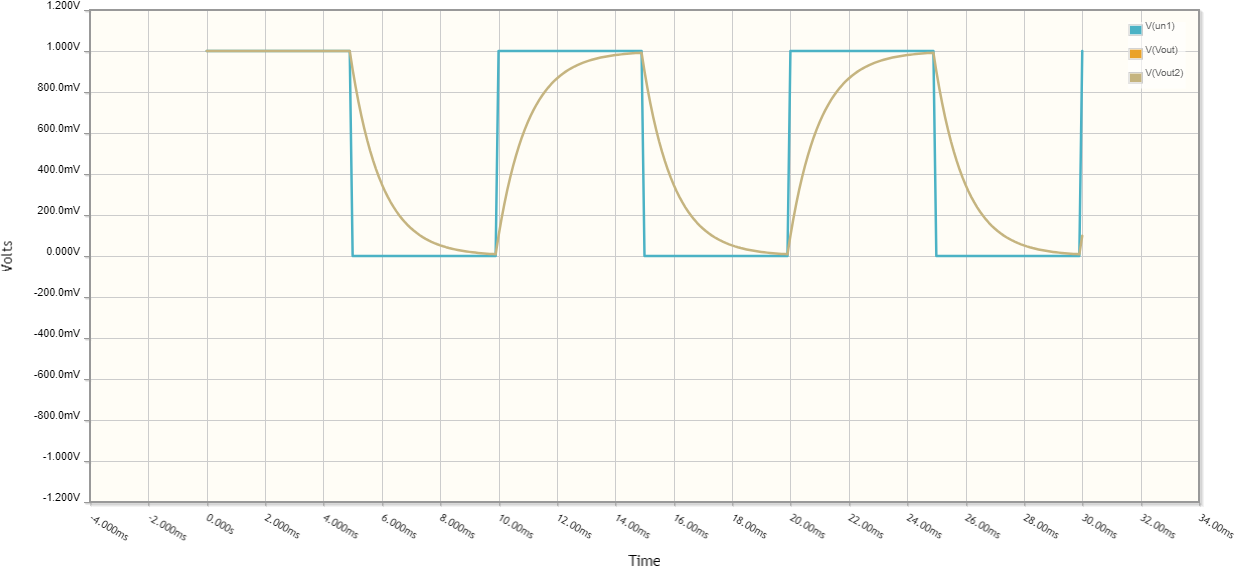
\includegraphics[width=0.5\textwidth]{images/Lowpassfilter1.png}
\end{multicols}

Think about how the capacitor will behave. At time $t=0$, the capacitor is fully charged. No current will flow at this time, meaning it will act as an open circuit, and therefore have a ``resistance" of $\infty$. You can think of the circuit as being like a voltage divider whose $R_2 = \infty$, and or $\Vo = \Vi$. At $t = (1/2)\omega$, the capacitor is able to discharge, and dissipates charge according to its decay curve. At $t = \omega$, the capacitor is subject to voltage again and begins to charge up. At first it acts like a wire, since it draws current proportional to the input voltage. As it becomes fully charged, it will again act like an open circuit.\newline

Let's now consider swapping positions: 

\begin{multicols}{2}
    \begin{center}
    \begin{circuitikz}
    \draw 
    (1,2) to [R, l=1 k$\Omega$] (1,0)
    (-2,2) to [sqV] (-2,0)
    (-2,0) -- (0,0)
    (1,2) to [short, -*] (3,2)
    (-2,2) to [C, l=1 $\mu$F] (1,2) 
    (3,0) to [short, *-] (0,0)
    (3,2.5) node {$\Vo$};;
    \end{circuitikz}
    \end{center}
    
    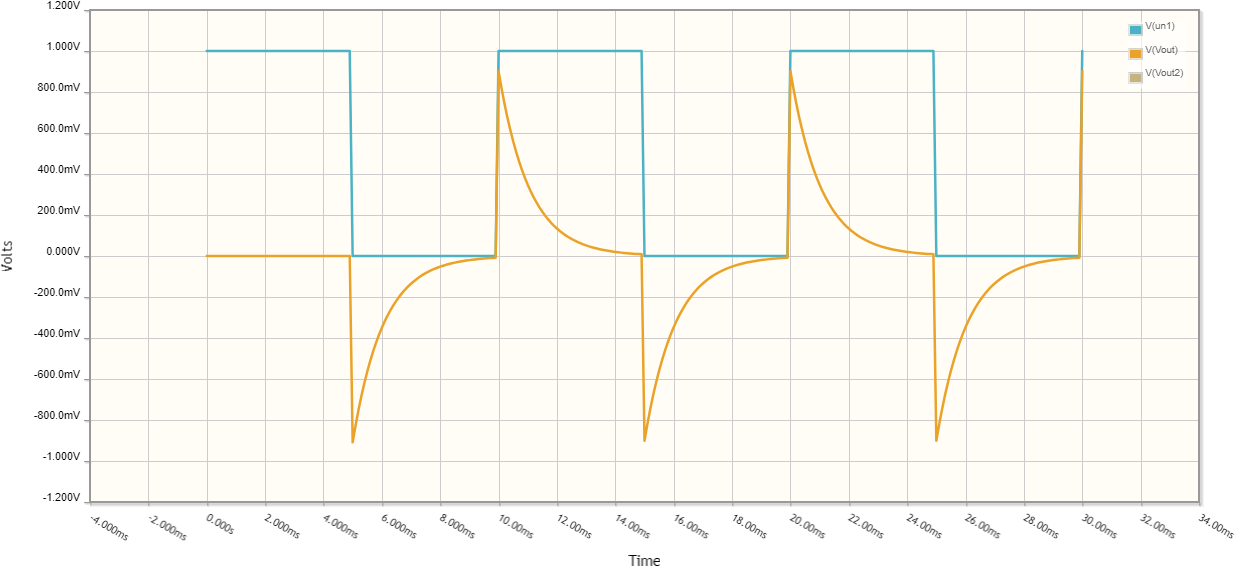
\includegraphics[width=0.5\textwidth]{images/Highpassfilter1.png}
\end{multicols}

At $t=0$, the capacitor is fully charged, so no current flows at all, and $\Vo = 0$. This is expected, since capacitors are meant to filter out DC voltage. At $t = (1/2)\omega$, the capacitor shoots down to $-\Vpp$. This is because $\Vi$ becomes negative relative to the voltage that the capacitor is held at. I.e., one plate of the capacitor is held at this $\Vpp$ value, so when $\Vi$ goes to 0, the voltage is negative between the plates of the capacitor, which draws negative current to the plate on the right side, making the voltage drop across the 1k$\Omega$ resistor equal to $-IR$. It then undergoes its standard decay curve, following this rule. Again, the decay will end at 0 because capacitors filter out DC voltage. 


\section{Filtration Conceptually}

Firstly, what is filtration? Filtration refers to our filtering out of background signal, or any undesired signal, in order to isolate our signal of interest. For example, perhaps you are interested in a sine wave whose period is 1 ms, but this is superimposed on a bunch of other sine waves of variable periods. You can extract the 1ms sine wave with some clever circuits, and build your downstream circuit fragments based on it. It's like an analog version of the Fourier Transform!\newline 

Let's consider a specific example given by Professor Ashmanskas: imagine you are building a sensor that tests the water level in a pool. You don't want the pool to overflow when it rains, or get too low when the Summer comes and water evaporates---so you devise an automatic system to add or take out water as needed. One could simply add a sensor to the side of the pool, but it will be subject to the constant waves formed by people swimming, and its readings will be horribly variable and uninterpretable, as they do not reflect the so-called \textit{steady-state} value of the water level. Each time someone cannon-balls in and splashes it, the sensor will think that the pool is greatly overflowing. Thus, one can devise a circuit that filters out all of these little fluctuations (this would be called a \textit{low-pass filter}, for passing variations that occur on a long time-scale---low frequency).


\subsection{Integration and Differentiation}
Capacitors have this incredible ability to perform complex math, including taking derivatives or integrals of your wave form. Let's think about how this may occur using the circuit mentioned in the previous part. Firstly, recall that the current flowing through the resistor must equal the current flowing through the capacitor, and that $Q = CV$: 

\begin{multicols}{2}
\begin{center}
\begin{circuitikz}
\draw 
(1,2) to [C, l=C$_1$] (1,0)
(-2,2) to [sV, l=V$_{in}$] (-2,0)
(-2,0) -- (0,0)
(1,2) to [short, -*] (3,2)
(-2,2) to [R, l=R$_1$] (1,2)
(3,0) to [short, *-] (0,0)
(3,2.5) node {V$_{out1}$};
\end{circuitikz}
\end{center}

\begin{center}
\begin{circuitikz}
\draw 
(1,2) to [R, l=R$_2$] (1,0)
(-2,2) to [sV, l=V$_{in}$] (-2,0)
(-2,0) -- (0,0)
(1,2) to [short, -*] (3,2)
(-2,2) to [C, l=C$_2$] (1,2)
(3,0) to [short, *-] (0,0)
(3,2.5) node {V$_{out2}$};
\end{circuitikz}
\end{center}
\end{multicols}


We can then solve for the voltage drop across R$_1$ as: 

\begin{equation} \label{cap2}
\begin{split}
{Q} &= {C_1V}_{out1}\\
\frac{d}{dt}{Q} &= \frac{d}{dt}{C_1V}_{out1} \\
{I} &= {C_1}\frac{d{V}_{out1}}{dt} \\
\end{split}
\end{equation}
\begin{equation} \label{cap3}
\begin{split}
{IR}_1 &= V_{in} - V_{out1} \\
\frac{d{V}_{out1}}{dt} &= \frac{1}{{R}_1 C_1}\pr{V_{in} - V_{out1}}
\end{split}
\end{equation}\newline

Therefore, if V$_{out}$ is very small compared to V$_{in}$, you get: 

\begin{equation} \label{cap4}
\begin{split}
\frac{d{V}_{out1}}{dt} &= \frac{1}{{R}_1 C_1}V_{in}\\
\int \frac{d{V}_{out1}}{dt} &= \int \frac{1}{{R}_1 C_1}V_{in}\\
{V}_{out1} &= \frac{1}{{R}_1 C_1} \int V_{in}\\
\end{split}
\end{equation}

And or, that $\V_{out}$ integrates $\V_{in}$. How will this change if we swap the positions of the resistor and capacitor in circuit 2? Once again, consider when $\V_{out}$ is much smaller than the input. 

\begin{equation} \label{cap5}
\begin{split}
{I} &= {C_2}\frac{d}{dt} \pr{V_{in} - V_{out2}}\\
{\frac{V_{out2}}{R_2}} &= {C_2}\frac{d}{dt} \pr{V_{in} - V_{out2}}\\
{\frac{V_{out2}}{R_2}} &= {C_2}\frac{d V_{in}}{dt}\\
V_{out2} &= R_2{C_2}\frac{d V_{in}}{dt}\\
\end{split}
\end{equation}\newline

Thus, in this case $\V_{out}$ approximates the derivative of $\V_{in}$. 

\subsubsection{Qualitative Thinking.}

The best lead in to thinking about filtration, to me, is thinking simply about how the graphs look like when something integrates or differentiates a square wave, combined with our understanding of capacitor behavior from above. Let us not do any math, and think only qualitatively.\newline 

\begin{centering}
\begin{tikzpicture}
\begin{axis}[
    xlabel=time,
    ylabel=voltage,
    xmin=0, xmax=10,
    ymin=0, ymax=10,
    xtick={0},
   % <---
    ytick={0}
            ]
% can add points by inserting ,mark=* into the specifications
\addplot[color=green]
    plot coordinates {
    (0,0)
    (2,0)
    (2,8)
    (8,8)
    (8,0)
    (10,0)
    };
\addplot[smooth,color=red]
    plot coordinates {
    (2,0)
    (3,5)
    (5,7)
    (8,8)
    };
\addplot[smooth,color=blue]
    plot coordinates {
    (2,4)
    (3,1)
    (4,0.25)
    (8,0)
    };
\end{axis}
    \end{tikzpicture}
    
\end{centering}

If the green waveform is our $\V_{in}$ from the previous example, then our red curve is similar to how $\V_{out1}$ may look, and the blue curve is similar to how $\V_{out2}$. That is, the blue curve \textit{kind of} differentiates the green curve, because the relatively instant rise signifies a very positive derivative, marked by this blue spike. Similarly, the red curve \textit{kind of} integrates the green curve, because the area under the green curve slowly accumulates, hence the overall positive slope of the red curve.\newline 

Something interesting you might notice, though, about the blue curve is that it seems centered around 0, while the red curve seems centered around the midway point of the green $\Vi$. You can realize that the capacitor being before $\Vo$ means it'll filter out all DC voltage, thereby centering $\Vo$ about 0. Thus, you can expect there to be a symmetric, negative curve on the downward edge of the green curve, as mentioned and discussed in section \textbf{\ref{sec:CapacitorBehavior}}.\newline

So if we say that the frequency is extremely slow, and the red curve is the voltage being measured at $\V_{out2}$, how might the red curve look? 

\begin{multicols}{2}
\begin{tikzpicture}
\begin{axis}[
    xlabel=time (low frequency),
    ylabel=voltage,
    xmin=0, xmax=10,
    ymin=0, ymax=10,
    xtick={0},
   % <---
    ytick={0}
            ]
% can add points by inserting ,mark=* into the specifications
\addplot[color=green]
    plot coordinates {
    (0,0)
    (2,0)
    (2,8)
    (8,8)
    (8,0)
    (10,0)
    };
\addplot[smooth,color=red]
    plot coordinates {
    (2,0)
    (2.2,5)
    (2.6,7)
    (3,8)
    };
\addplot[smooth,color=red]
    plot coordinates {
    (8,8)
    (8.2,7)
    (8.6,5)
    (9,0)
    };
\addplot[color=red]
    plot coordinates {
    (8,8)
    (3,8)
    };
\end{axis}
    \end{tikzpicture}

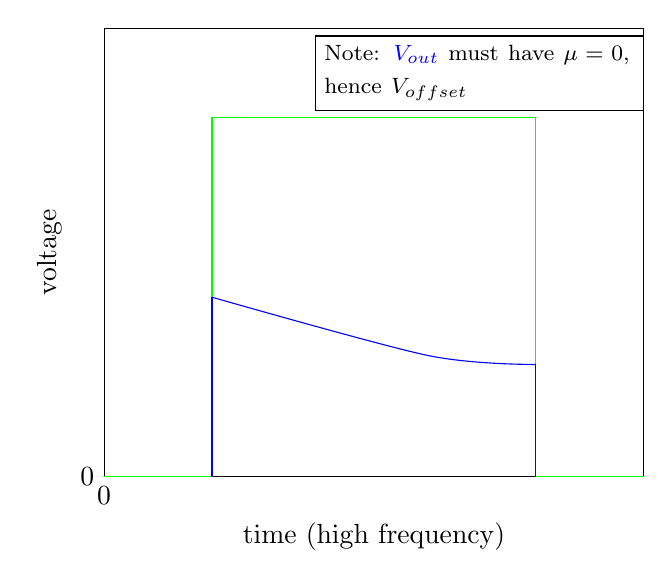
\begin{tikzpicture}
\begin{axis}[
    xlabel=time (high frequency),
    ylabel=voltage,
    xmin=0, xmax=10,
    ymin=0, ymax=10,
    xtick={0},
   % <---
    ytick={0}
            ]
% can add points by inserting ,mark=* into the specifications
\addplot[color=green]
    plot coordinates {
    (0,0)
    (2,0)
    (2,8)
    (8,8)
    (8,0)
    (10,0)
    };
\addplot[smooth,color=blue]
    plot coordinates {
    (2,4)
    (6,2.7)
    (8,2.5)
    };
\addplot[color=blue]
    plot coordinates {
    (2,0)
    (2,4)
    };
\addplot[color=blue]
    plot coordinates {
    (8,0)
    (8,2.5)
    };
\node[draw,text width=4cm] at (7,9) {\footnotesize Note: \textcolor{blue}{$\Vo$} must have $\mu = 0$, hence $V_{offset}$};
\end{axis}
    \end{tikzpicture}    
\end{multicols}

Similarly, if the frequency is very high, how might the blue curve look? Take a second to ponder the two graphs above and gather a bit of intuition on it. This should allow you to qualitatively state that an integrating circuit will be a \textit{low-pass filter} (because $\Vo$ matches $\Vi$), and a differentiating circuit will be a \textit{high-pass filter} (except that there's an offset when the long-term average of $\Vi \neq 0$). As in the left graph, as the frequency gets smaller and smaller, the red plot will more and more closely match the green plot. This is the basis of capacitor filtration, an essential tool in electronics!

\section{Frequency Dependence}
This section will primarily be quantitative. The important bits, though, are the qualitative understandings, and the final results of this quantitative section. What you find in the interim is likely not worth understanding fully. Let's begin by supposing we apply a $\cos$ wave to a resistor. The relationship between current and voltage is as follows:

\begin{equation} \label{freq1}
\begin{split}
f &= \frac{\omega}{2\pi}\\
V(t) &= \Vpp \cos\pr{\omega t} \\
V(t) &= I(t)\mathrm{R} \\
I(t) & = \pr{\Vpp / {R}} \cos\pr{\omega t}\\
\end{split}
\end{equation}\newline

Therefore, if you were to solve something like $\Vo / \Vi$ your pesky $\cos$ terms will cancel. This simply means that $\Vi$ and $\Vo$ will be in phase, only changed by some scaling factor. Unfortunately, this is not so for capacitor equations. We can see this below: 

\begin{equation} \label{freq2}
\begin{split}
Q &= CV \\
I(t) &= C \frac{d \pr{\Vpp \cos\pr{\omega t}}}{dt} \\
I(t) &= - \omega C \Vpp \sin \pr{\omega t} \\
\end{split}
\end{equation}\newline

This means that the current and the voltage will be $90^{\circ}$ out of phase. Another way would be to write this as $A \cos \pr{\omega t + \phi}$. Let us think about what will happen with our standard low-pass filter. Using KVL, we can state that: 

\begin{equation} \label{freq3}
\begin{split}
\Vpp \cos\pr{\omega t} &= RC\frac{dv_C}{dt} + v_c \\ 
v_c &= A \cos \pr{\omega t + \phi} \\ 
\Vpp \cos\pr{\omega t} &= RC\frac{d}{dt}A \cos \pr{\omega t + \phi} + A \cos \pr{\omega t + \phi} \\
\end{split}
\end{equation}


\subsection{Imaginary Numbers Digression.}
Maybe looked at the previous equation and thought it is solvable (probably?) but that it would be not worth your while to do so, and that there is likely a better way to go about it. Recall Euler's Relation\footnote{Electrical Engineers use $j$ instead of $i$ for imaginary numbers. The claim is that it is easier to keep track of in the math. Other's claim it's because $i$ is sometimes used to represent currents, particularly small ones.}: 

\begin{equation} \label{imag1}
\begin{split}
e^{j\omega t} = \cos(\omega t) + j\sin(\omega t) \\
\end{split}
\end{equation}

One of the requirements of a linear circuit is superposition, and that is \textit{kind of} the argument that allows us to use imaginary numbers. You can think that if you are using math that includes both a real and imaginary component, as long as you keep track of the real, your output will still be correct---but, don't think too hard about this. In the upcoming sections, I will use \textbf{v}$_c$ to denote the complex number. Let us examine: 

\begin{equation} \label{imag2}
\begin{split}
\Vpp e^{j\omega t} &= RC\frac{d\textbf{v}_c}{dt} + \textbf{v}_c \\
\textbf{v}_c &= Ae^{j\omega t} \\
\Vpp e^{j\omega t} &= RC\frac{d}{dt}Ae^{j\omega t} + Ae^{j\omega t} \\
\end{split}
\end{equation}

We can differentiate, and then obtain an expression for $A$, and solve for the voltage at the capacitor as:

\begin{equation} \label{imag3}
\begin{split}
\Vpp e^{j\omega t} &= j\omega RCAe^{j\omega t} + Ae^{j\omega t} \\
\Vpp &= j\omega RCA + A \\
\Vpp &= A\pr{1 + j\omega RC}\\
\frac{\Vpp}{\pr{1 + j\omega RC}} &= A\\
\textbf{v}_c &= \frac{\Vpp}{1 + j\omega RC}e^{j\omega t} \\
\end{split}
\end{equation}

We now want to find the real component, which begins by rewriting the expression in its polar form: 

\begin{equation} \label{imag4}
\begin{split}
\textbf{v}_c &= \pr{\frac{1}{\sqrt{1 + \omega^2 R^2C^2}}e^{j\phi}}\Vpp e^{j\omega t} \\
\phi &= \tan^{-1}(-\omega RC) \\
\textbf{v}_c &= \frac{1}{\sqrt{1 + \omega^2 R^2C^2}}\Vpp e^{j(\omega t + \phi)} \\
\end{split}
\end{equation}

From here we can simply take the real part and be on our way:

\begin{equation} \label{imag5}
\begin{split}
v_c &= \frac{\Vpp}{\sqrt{1 + \omega^2 R^2C^2}} \cos(\omega t + \phi) \\
\end{split}
\end{equation}

This is equivalent to saying:

\begin{equation} \label{imag5}
\begin{split}
A_{out} &= A_{in}\sin(\omega t + \phi) \\
\end{split}
\end{equation}

Where $A$ is the amplitude at either time. This is one way to go about this problem. Another way, which will be discussed in the next section, is using impedance. 

\section{Impedance}
We mentioned earlier in equation \eqref{imag3} that the relationship between an input voltage and what is measured at a capacitor for a low-pass filter is: 

\begin{equation} \label{imp1}
\begin{split}
\Vi \frac{1}{1+j\omega RC} = v_c
\end{split}
\end{equation}

If we were to divide this fraction by $j\omega C$, and simplify using the representation $Z_C$, we would get: 

\begin{equation} \label{imp2}
\begin{split}
\Vi \frac{1/j\omega C}{1/j\omega C + R} = v_c \\
\Vi \frac{Z_C}{Z_C + R} = v_c \\ 
\end{split}
\end{equation}

This looks just like a voltage divider equation! The concept of \textit{impedance} is used to summarize other circuit fragments, like capacitors or inductors, using some resistance equivalent $Z$. The impedance of a resistor, $Z_R$, is simply R. $Z_C$ is ${1} / j\omega C$. Let's think of how this pertains to our low-pass filter. 

\begin{center}
\begin{circuitikz}
\draw 
(1,2) to [C, l=C] (1,0)
(-2,2) to [sV, l=V$_{in}$] (-2,0)
(-2,0) -- (0,0)
(1,2) to [short, -*] (3,2)
(-2,2) to [R, l=R] (1,2)
(3,0) to [short, *-] (0,0)
(3,2.5) node {V$_{out}$};
\end{circuitikz}
\end{center}

If we measure at $\Vo$, we can think of it like a voltage divider, giving us: 

\begin{equation} \label{imp3}
\begin{split}
\Vo = \frac{Z_C}{Z_C + R}\Vi
\end{split}
\end{equation}

You may wonder if $Z_C = {1} / j\omega C$ has any real basis, or if it is simply an extraction from the above math. In reality, you can find it quite simply through: 

\begin{equation} \label{imp4}
\begin{split}
I_c = C\frac{dv_c}{dt} \\
I_ce^{j\omega t} = CA\frac{d}{dt}e^{j\omega t} \\
I_ce^{j\omega t} = j\omega CAe^{j\omega t} \\
I_c = j\omega CA \\
I_c\frac{1}{j\omega C} = A \\
\end{split}
\end{equation}

This is the equivalent of Ohm's law, where ${1} /{j\omega C}$ is the resistance. Understanding this, we can find our high-pass filter's equation to be: 

\begin{equation} \label{imp5}
\begin{split}
\Vo = \frac{R}{Z_C + R}\Vi
\end{split}
\end{equation}

\section{Filtration Quantitatively}
We are finally prepared to talk about filtration quantitatively! As was mentioned in the impedance discussion, resistor-capacitor (RC) circuits can be formulated as voltage dividers. We know that the impedance of a capacitor is ${1} /{j\omega C}$, which has some frequency dependence from $\omega$ (or, $2\pi f$). Therefore, we can get the sense that $\Vo$ may change depending on this frequency. With a bit of re-writing, we find: 

\begin{equation} \label{imp6}
\begin{split}
\frac{\Vo}{\Vi} &= \frac{Z_C}{Z_C + R} \\
\frac{\Vo}{\Vi} &= \frac{1}{1 + j\omega RC} \\
\frac{\Vo}{\Vi} &= \frac{1}{\sqrt{1 + (2\pi f RC)^2}} \\
\end{split}
\end{equation}

We can see that as the frequency goes up, this converges to $1 / \infty$, or $1/1$ as frequency goes down. Whereas, for a high pass filter: 

\begin{equation} \label{imp7}
\begin{split}
\frac{\Vo}{\Vi} &= \frac{R}{Z_C + R} \\
\frac{\Vo}{\Vi} &= \frac{j\omega RC}{1 + j\omega RC} \\
\frac{\Vo}{\Vi} &= \frac{2\pi f RC}{\sqrt{1 + (2\pi f RC)^2}} \\
\end{split}
\end{equation}

Which converges to $\infty / \infty$ as frequency goes up, and $0 / 1$ as frequency goes down.

\subsection{Corner Frequency and Phase Shift}
The way one quantifies this is with the ``corner frequency," which you will more often hear as $\fdb$. You'll notice that for both the high-pass and low-pass filter equations described above, the ratio of $\Vo$ to $\Vi$ is $1/\sqrt{2}$ when the frequency inputted is $f = 1/2\pi RC$. $1/\sqrt{2}$ corresponds to about 0.7, meaning that at this $\fdb$, the output is about 70\% the amplitude of the input. Thus, it is a good marker of how well your filter will work. If you are trying to pick a low pass filter that filters out anything at 1000 kHz and higher, you'll want to pick an RC circuit combination that is well below it.\newline

Notably, filtration causes a phase shift. This shouldn't be surprising when you recall that a low-pass and high-pass filter also integrate and differentiate respectively. Let us take, for example, a $\sin$ input. If it is passed through a low-pass filter, would expect it to be integrated to $-\cos$. If passed to a high-pass, it would be differentiated to $\cos$. Therefore, as $-\cos$ is $-90^{\circ}$ ($\sin(x - \frac{\pi}{2}) = -\cos(x)$) relative to $\sin$, and $\cos$ is $+90^{\circ}$ ($\sin(x + \frac{\pi}{2}) = \cos(x)$), we would expect a low-pass filter to generate an output that lags $\Vi$, while a high-pass will generate one which precedes $\Vi$.\newline

The filtration at $\fdb$ is $45^{\circ}$. I don't think this has a straightfoward math explanation, but conceptually it is when the real and imaginary parts are equal. Maybe don't think about this too hard. 

\subsection{Summarizing Thoughts}

\begin{multicols}{2}
\begin{center}
\begin{circuitikz}
\draw 
(1,2) to [C, l=C$_1$] (1,0)
(-2,2) to [sV, l=V$_{in}$] (-2,0)
(-2,0) -- (0,0)
(1,2) to [short, -*] (3,2)
(-2,2) to [R, l=R$_1$] (1,2)
(3,0) to [short, *-] (0,0)
(3,2.5) node {V$_{out1}$};
\end{circuitikz}
\end{center}

\begin{center}
\begin{circuitikz}
\draw 
(1,2) to [R, l=R$_2$] (1,0)
(-2,2) to [sV, l=V$_{in}$] (-2,0)
(-2,0) -- (0,0)
(1,2) to [short, -*] (3,2)
(-2,2) to [C, l=C$_2$] (1,2)
(3,0) to [short, *-] (0,0)
(3,2.5) node {V$_{out2}$};
\end{circuitikz}
\end{center}
\end{multicols}

Let us look at these two circuits again, and see what we can tell just from a glance.\newline

For the left circuit, since the current through the resistor and capacitor must be the same, we can say $Q = C\Vo$, and thus $I = C\Vo'$, that $\Vi = IR = RC\Vo'$, so $\Vo$ integrates $\Vi$. Knowing that it integrates, we can intuit that it must be a low-pass filter, based on the graphs presented earlier. We can also know it is a low-pass filter if we recall that $Z_C = 1/j\omega C$, and that a voltage divider must look like $Z_C / R + Z_C$, which would give us $1 / j\omega C + 1$. And, since it integrates, we know that $\int \sin = -\cos$, so there will be a $-90^{\circ}$ phase shift at very high frequencies.\newline

For the right circuit, since $\Vi - \Vo = V_C$, we know $CV_C' = I$, so $\Vo = RC\Vi'$. Therefor, it differentiates, which means it mus be a high-pass filter. Too, it must be of the form $R/Z_C + R$. And if it differentiates, then $\sin ' = \cos$, so there must be a $+90^{\circ}$ phase shift at very low frequencies.\newline

In other words, you can tell a lot just at a glance! This is without any math!

\section{Inductors}
An inductor stores energy in a magnetic field. An inductor is usually a tightly coiled bit of wire, and as you know a wire always has a magnetic field, so by coiling them and running current through it, you are summing these magnetic fields.\newline

To conceptualize an inductor's behavior, as we will consider a water-wheel. An inductor is like a water-wheel in a pipe. As water flows through the pipe and reaches this large, heavy wheel, the speed of flow will be decreased as this wheel is pushed. Eventually, the wheel gets `up to speed' so-to-speak, and its momentum carries it. The water's flow will not be impeded at this point. If you were to stop the flow of water, the momentum of the wheel would allow it to continue spinning, thereby continuing the water's movement for a time. If you were to have an LED in parallel with an inductor, you would expect that the LED would initially shine very brightly, as the inductor functions similarly to a large resistor its early stages. You'll see the LED dim as the inductor becomes fully charged, and now acts like a wire. If you remove the battery from the circuit, the LED will remain on for a time, as the inductor loses its charge. The rate at which the inductor dissipates its charge will depend on the total resistance of the circuit.\newline

In fact, the magnetic field that forms as a reduce of current generates an electromotive force in the opposite direction, essentially opposing the current's flow. This field is held for some time constant, similar to a capacitor. An inductors time constant is $\tau = 2L/R$. The field is generated at at a rate of $V = L\frac{d}{dt}I$, compared to a capacitor's curve of $I = C\frac{d}{dt}V$. Therefore, you can imagine that an inductor may work opposite of a capacitor. Indeed, the impedance of an inductor is $j\omega L$, compared to a capacitors $1/ j\omega C$. The $\fdb$ in this case is $R/2\pi L$. Inductors act like resistors, in that you can add them up in series like resistors, and treat them as you would with resistors in parallel. However, when we consider only impedance, everything functions like a resistor. That makes analyzing our below circuit much nicer. 

\begin{center}
\begin{circuitikz}
\draw 
(1,2) to [R] (1,0)
(-4,2) to [sV] (-4,0)
(-4,0) -- (0,0)
(1,2) to [short, -*] (3,2)
(-2,2) to [C] (1,2)
(-4,2) to [inductor] (-1,2)
(3,2.5) node {V$_{out}$}
(3,0) to [short, *-] (0,0);
\end{circuitikz}
\end{center}

This can be solved as $Z_2/Z_1 + Z_2$, where $Z_2 = R$, and $Z_1 = j\omega L + 1/j\omega C$. Let me try a bit of math here: 

\begin{equation} \label{filt1}
\begin{split}
Z_1 &= j\omega L + \frac{1}{j\omega C} \\
Z_1 &= \frac{-\omega^2 LC}{j\omega C} + \frac{1}{j\omega C} \\
Z_1 &= \frac{1 -\omega^2 LC}{j\omega C}\\
\end{split}
\end{equation}

The impedance, $Z_1$, goes to zero when $\omega^2 LC = 1$. In other words, at some frequency, $f_0$, the impedance will be minimized. This is called the resonant frequency, and is found at $f_0 = 1/2\pi \sqrt{LC}$. You can think about what would happen when the inductor and capacitor are in parallel in the circuit above:

\begin{equation} \label{filt2}
\begin{split}
Z_1 &= j\omega L \: || \: \frac{1}{j\omega C} \\
Z_1 &= \frac{j\omega L/j\omega C}{j\omega L + 1/j\omega C} \\
Z_1 &= \frac{j\omega L}{1-\omega^2 LC} \\
\end{split}
\end{equation}

Now, impedance will go to infinity at the described $f_0$---and you can filter out a specific frequency. It is useful to know how this filtering will affect the power dissipated by your circuit. At $\pm \Delta f = R/2\pi L$, the power halves, so one would call the bandwidth of this circuit to be $2\Delta f$. A halved power corresponds to an amplitude decrease of $1/\sqrt{2}$ (since $P = V^2/R$). Thus, at the two sides of the bandwidth, you'd expect to see an amplitude that is about $70\%$ as large as at $f_0$. 

\subsubsection{Either or?}
So why are capacitors much more widely used than inductors? To start, inductors are usually large and heavy. As it must be a coin of wires, usually wrapped around some magnetically-permeable metal, it doesn't easily fit into circuit boards. Too, inductors will continuously dissipate energy, while capacitors that are charged do not.\newline

\section{Peak Detection}

An interesting application of a low-pass filter is peak detection. There may be times where you are only interested in extremes, and not the little fluctuations in between. For example, perhaps you're interested in neural activity. You probably don't care too much about individual peaks, but instead you want to get a measure of the overall activity. This is one such way to do so\footnote{These two examples are from Tom Hayes' Chapter 3N.}: \vfill\pagebreak

\begin{multicols}{2}
    
\begin{center}
\begin{circuitikz}
\draw 
(0,0) to[diode, *-] (2,0) coordinate(diode)
to[R] ++(2,0) coordinate(resistor)
to[C] ++(0,-2)
node[ground]{}
(diode) to[R] ++(0,-2)
node[ground]{}
(resistor) to[short, -*] ++(1,0) node[above] {$\Vo$}
(0,0) node[above] {$\Vi$}
;
\end{circuitikz}
\end{center}


\begin{center}
\begin{circuitikz}
\draw 
(0,0) to[diode, *-] (2,0) coordinate(diode)
to[short] ++(2,0) coordinate(resistor)
to[R] ++(0,-2)
node[ground]{}
(diode) to[C] ++(0,-2)
node[ground]{}
(resistor) to[short, -*] ++(1,0) node[above] {$\Vo$}
(0,0) node[above] {$\Vi$}
;
\end{circuitikz}
\end{center}

\end{multicols}


You can conceptually imagine that to create some form of peak detection, you want the $RC$ decay value to be slow relative to the minute fluctuations, but fast relative to the longer term fluctuations you are interested in capturing. 


\section{Input and Output Resistance}

Now that we have a better understanding of impedance, let's discuss the idea of input and output resistance again. This concept is actually quite interesting and important, because when you are supplying a voltage to the body (say, in stimulating the spinal cord) you'll see impedance drifts, and phase shifts over time. Therefore, having a strong conceptual understanding of voltage sources \& sinks, and input \& output resistances is useful in quantifying this.\newline

So for: 

\begin{center}
\begin{circuitikz}
\draw 
(0,2) to [battery, l_=$V_{th}$] (0,0)
(0,2) to [R, l=$R_{th}$,-*] (3,2) node[right] {A}
(3,0) to [short, *-] (0,0) 
(3,0) to [R,l_=$R_{in}$] (3,2)
(3,0) node[right] {B}

;
\end{circuitikz}
\end{center}


We get: 

\begin{multicols}{2}



\begin{center}
\begin{tikzpicture}
\begin{axis}[
    xlabel=$I_{out}$,
    ylabel=$V_{out}$,
    xmin=0, xmax=30,
    ymin=0, ymax=100,
    xtick={0},
    ytick={0}
            ]
\addplot[smooth,color=red]
    plot coordinates {
        (15,0)
        (7.5, 45)
        (0,90)
    };
    \draw (3,90) node {$V_{oc}$};
    \draw (15,10) node {$I_{sc}$};
    \draw (13,50) node {Slope = $-R_{th}$};
\end{axis}
\end{tikzpicture}
\end{center}



\begin{center}
\begin{tikzpicture}
\begin{axis}[
    xlabel=$I_{out}$,
    ylabel=$V_{out}$,
    xmin=0, xmax=30,
    ymin=0, ymax=100,
    xtick={0},
    ytick={0}
            ]
\addplot[smooth,color=red]
    plot coordinates {
        (0,0)
        (7.5, 45)
        (15,90)
    };
    \draw (16,50) node {Slope = $1/R_{in}$};
\end{axis}
\end{tikzpicture}
\end{center}

   
\end{multicols}

The left graph was presented in an earlier section. The important takeaway is that for a linear system, $R_{th} = -\Delta V_{\mathrm{AB}}/\Delta I_{\mathrm{A}}$. For a non-linear system, we can generalize this to include the impedance: 


\begin{equation} \label{out}
\begin{split}
Z_{out} = -\frac{dV_{AB}}{dI_A}\\
\end{split}
\end{equation}

Where $V_{AB}$ is across the voltage source, and $I_A$ is from the voltage source, and when we are varying the load resistance. Then, the input resistance of the load can be defined as: 


\begin{equation} \label{in}
\begin{split}
\frac{1}{Z_{in}} = \frac{dI_{A}}{dV_{AB}}\\
\end{split}
\end{equation}

For the $I_A$ into the load and the $V_{AB}$ across the load when we are varying the voltage source. 


\textcolor{red}{The next section should be diodes/LEDs, but I find those to be just so boring. So I'd rather skip to opamps.}

\vfill

\chapter{Opamps}

Operational amplifiers (opamps) are one of the most ubiquitous tools in electronics, just behind classics like the resistor and capacitor. While they themselves are amazing, making CircuitTikz diagrams for them is a nightmare! So wish me luck in the coming parts!\newline

As there are countless opamp applications, it can become muddled why you'd want a circuit to do such things. Thus, I'll do my best to think of interesting biological applications for the less obvious ones. 

\section{Introduction and Gold}

Opamps are active components, in that they can take a circuit's power and increase it. They have the ability to amplify signal, act as a voltage clamp, do addition and subtraction, and even integration and differentiation. Let's discuss:

\begin{center}
\begin{circuitikz} 
\draw
(0,0) node[op amp] (opamp) {}
(opamp.+) node[left] {$v_+$}
(opamp.-) node[left] {$v_-$}
(opamp.out) node[right] {$\Vo$}
(opamp.up) --++(0,0.5) node[vcc]{$+V$}
(opamp.down) --++(0,-0.5) node[vee]{$-V$}
;
\end{circuitikz}
\end{center}

Inside of an opamp is a large network of transistors. It isn't worth trying to understand all the internals, but it is worth understanding all of the externals. An opamp has two inputs ($v_-$ and $v_+$), and two power rails ($+V$ and $-V$). In general, an opamp's goal will be to minimize the difference between the two inputs, and it has some range of power to work with in doing so, which is limited by $+V$ and $-V$. It tries to minimize this input through its $\Vo$. Therefore, one would often connect the $v_-$ to $\Vo$ as a form of negative feedback. This will likely make more sense in the later sections. If there is no connection between $\Vo$ and either of the two inputs, your opamp will oscillate between the two power maximums set by $+V$ and $-V$. As in, if $v_- > v_+$, then $\Vo = +V$. This is an opamp functioning as a \textit{comparator}, in that it makes the somewhat binary comparison of which input is larger, and outputs either high or low voltage. 


\subsection{Golden Rules}
In adding some form of negative feedback, and keeping your opamp from being saturating (i.e., clamping $\Vo$ to either of the two power rails)\footnote{These two specifications are sometimes called the 0$^\mathrm{th}$ rule.}, an opamp will adhere to two essential rules:

\begin{enumerate}
    \item $\Vo$ does whatever needed to ensure $v_+ = v_-$. 
    \item $v_+$ and $v_-$ draw no current.
\end{enumerate}

\section{Simple Opamp Circuits}

Implicit in rule two is that an opamp has immensely high resistance. That means that the input resistance seen by earlier circuit components is effectively an open circuit ($R = \infty$) for an ideal opamp. The simplest opamp circuit is seen as follows\footnote{Get it?}: 

\begin{center}
\begin{circuitikz} 
\draw
(0,0) node[op amp](F1-OA){} (opamp) {}
(opamp.+) node[left] {}
to[short, -*] ++(-1,0) node[above] {$\Vi$}

(opamp.-) node[left] {}
to[short] ++(0,1)

(opamp.out) node[right] {}
to[short] ++(0,1.5)
to[short] ++(-2.4,0)
(opamp.out) to[short, -*] (2,0) node[above] {$\Vo$}
;
\end{circuitikz}
\end{center}

This is called a \textit{follower}, or \textit{buffer}. In such diagrams, usually $-V$ and $+V$ are omitted. Based on our golden rules, $v_-$ should match $v_+$, and our ciruit shows $v_+ = \Vi$, so therefore $\Vo$ will be increased by the opamp until it reaches $\Vi$, because $v_-$ is tied to $\Vo$. The point being, the circuit followers as $\Vi = \Vo$. You might say ``\textit{so it's just a wire then?}" In many ways, you are correct! But here is a nice application that shows why a follower would be useful: 

\begin{center}
\begin{circuitikz}
\draw 
(1,2) to [R, l=2 k$\Omega$] (1,0)
(-2,2) to [battery, l=9 V] (-2,0)
(-2,0) -- (0,0)
(-2,2) to [R, l=1 k$\Omega$] (1,2)
(5,0) to [short, *-] (0,0)
(5,2) to [short, *-] (4,2)

(1,2) to [R, l=1 k$\Omega$] (4,2)
(4,2) to [R, l=2 k$\Omega$] (4,0);
\end{circuitikz}
\end{center}

Recall this circuit from before. The important principle we learned was that because the $R_{th}$ of the first divider was similar to the $R_{eq}$ of the second, you could not treat this as $\Vi \times \frac{2}{3} \times \frac{2}{3} $. However, if we do the following: 

\begin{center}
\begin{circuitikz}
\draw 
(0,2) to [battery, l=9 V] ++(0,-2)

(0,2) to [R, l=1 k$\Omega$] ++(2,0)
to [R, l=2 k$\Omega$] ++(0,-2) 

(0,0) to [short, -*] ++(9,0)

(6,2) to [R, l=1 k$\Omega$] ++(2,0)
to [R, l=2 k$\Omega$] ++(0,-2)
(8,2) to [short, -*] ++(1,0)

(4,2.5) node[op amp](opamp){} (opamp) {}

(opamp.+) node[left] {}
(opamp.+) node[left] {} 

(opamp.-) node[left] {}
to[short] ++(0,1)
(opamp.+) -| (2,2)

(opamp.out) node[right] {} 
to[short] ++(0,1.5)
to[short] ++(-2.4,0)
(opamp.out) |- (6,2)
;
\end{circuitikz}
\end{center}


Now, the first voltage divider will ``see" an input resistance of the opamp as being infinite. The opamp's output will be the voltage of the first voltage divider, and apply it to the second voltage divider. As such, we do get $\Vi \times \frac{2}{3} \times \frac{2}{3}$.\newline

$v_-$ is commonly called the \textit{inverting input}, because one can invert with it. An inverting follower would be seen as follows: 

\begin{center}
\begin{circuitikz} 
\draw
(0,0) node[op amp] (opamp) {}
(opamp.+) node[left] {}
to[short] ++(0,-0.5) node[ground]{}

(opamp.-) node[left] {}
to[short] ++(0,1)

(opamp.-) node[below] {$v_g$}
to[short, -*] ++(0,0)

(opamp.out) node[right] {}
to[short] ++(0,1.5)
to[short] ++(-2.4,0)
(opamp.-) node[right] {}
to[short, -*] ++(-1,0) node[above] {$\Vi$}
(opamp.out) to[short, -*] (2,0) node[above] {$\Vo$}
;
\end{circuitikz}
\end{center}

Intuitively, since $v_+$ is grounded (or, $V = 0\V$), to make $v_+ = v_-$, $v_-$ must equal $-\Vi$, and or, $\Vo = -\Vi$. Because of this, this node is sometimes called a \textit{virtual ground}, or $v_g$.\newline

Given some of these ideas, we can imagine some special opamp uses. Like:


\begin{center}
\begin{circuitikz}
\draw 
node[op amp, anchor=+](OA){}
(OA.-) to[R=$R_1$, -*] ++(-2,0) node[above]{$\Vi$}
(OA.-) to[short] ++(0,1) 
to[R=$R_2$] ++(2.5,0) 
to ++(0,-1.5) 

(OA.+) to[short] ++(0,0) node[ground]{}

(OA.out) to [short, -*] ++(1,0) node[above]{$\Vo$}
;
\end{circuitikz}
\end{center}

This is called an \textit{inverting amplifier}. Sometimes you'll see circuits like this overcomplicated in explanation. In reality, you should just recognize that the current across $R_1$ must equal the current across $R_2$, since no current flows into $v_-$. Automatically, this means since $\Vi = R_1I$, and $\Vo = -R_2I$ (due to direction of flow), you'll find that:

\begin{equation} \label{oa1}
\begin{split}
\Vo = -\frac{R_2}{R_1}\Vi
\end{split}
\end{equation}

A slightly more complex application is: 

\begin{center}
\begin{circuitikz}
\draw 
(0,0) node[above]{$\Vi$} to[short, *-] ++(1,0)
node[op amp, noinv input up, anchor=+](OA){}
(OA.-) -- ++(0,-1) coordinate(FB)
to[R=$R_1$] ++(0,-2) node[ground]{}
(FB) to[R=$R_2$, *-] (FB -| OA.out) -- (OA.out)
to [short, -*] ++(1,0) node[above]{$\Vo$}
;
\end{circuitikz}
\end{center}

This is called a \textit{non-inverting amplifier}. In this case, you can see that $R_1$ and $R_2$ form something of a voltage divider. That is, $V_- = R_1/(R_2 + R_1) \times \Vo$. Knowing that an opamp always wants to ensure $v_- = v_+$, we can say: 

\begin{equation} \label{oa2}
\begin{split}
\Vi & = \frac{R_1}{R_2 + R_1}\Vo \\
\Vi \pr{\frac{R_2}{R_1} + 1} & = \Vo \\
\end{split}
\end{equation}

The output resistance of an ideal opamp should be 0. That is, ideally an opamp would be able to drive any voltage irrespective of the current. The input resistance of the inverting amplifier will be whatever value we have for $R_1$, while the input resistance for the non-inverting amplifier is $\infty$, as it is directly connected to the opamp's $v_+$.\newline

Another thing you may wonder is if we can drive an infinite voltage at $\Vo$. Recall that we are limited by whatever voltage is provided to the opamp's power rails, shown at the start of this section.\newline

An expansion of the inverting amplifier is the \textit{summing amplifier}:

\begin{center}
\begin{circuitikz}
\draw 
node[op amp, anchor=+](OA){}
(OA.-) to[short] ++(-1,0) coordinate(cord)
(cord) to[short] ++(0,0.5)
to[R, l_=$R_1^A$, -*] ++(-2,0) node[above]{$V_A$}
(cord) to[short] ++(0,-0.5) 
to[R=$R_1^B$, -*] ++(-2,0) node[below]{$V_B$}
(OA.-) to[short] ++(0,1) 
to[R=$R_2$] ++(2.5,0) 
to ++(0,-1.5) 

(OA.+) to[short] ++(0,0) node[ground]{}

(OA.out) to [short, -*] ++(1,0) node[above]{$\Vo$}
;
\end{circuitikz}
\end{center}

The interpretation is largely the same. Given that all of the currents through individual resistors will sum together through $R_2$: 

\begin{equation} \label{oa3}
\begin{split}
\Vo & = -R_2 \pr{\frac{1}{R_1^A}V_A + \frac{1}{R_1^B}V_B} \\
\Vo & = -\frac{R_2 }{R_1^A}V_A - \frac{R_2 }{R_1^B}V_B \\
\end{split}
\end{equation}

Perhaps one application would be if you were interested in measuring the overall activity within the brain, and you are not so interested in discriminating individual electrodes in an EEG. Because the voltage changes measured by an EEG are so small, you'll need to amplify it. Thus, you throw them all together into a summing amplifier.\newline

Next is a \textit{differential amplifier} (not to be confused with derivative).

\begin{center}
\begin{circuitikz}
\draw 
node[op amp, anchor=+](OA){}
(OA.-) to[R, l_=$R_1^A$, -*] ++(-2,0) node[above]{$V_A$}
(OA.+) to[R=$R_1^B$, -*] ++(-2,0) node[below]{$V_B$}
(OA.-) to[short] ++(0,1) 
to[R=$R_2^A$] ++(2.5,0) 
to ++(0,-1.5) 

(OA.+) to[R=$R_2^B$] ++(0,-2) node[ground]{}

(OA.out) to [short, -*] ++(1,0) node[above]{$\Vo$}
;
\end{circuitikz}
\end{center}

Knowing that $v_- = v_+$, and that $v_- = V_A - I_AR_1^A$ and $v_- = \Vo + I_AR_2^A$: 

\begin{equation} \label{oa4}
\begin{split}
\frac{V_A - v_-}{R_1^A} &= \frac{v_- - \Vo}{R_2^A} \\
{R_2^A}(V_A - v_-) &= {R_1^A}(v_- - \Vo) \\
{R_2^A}V_A + {R_1^A}\Vo &= {R_1^A}v_- + {R_2^A}v_- \\
\frac{R_2^A}{R_1^A + R_2^A}V_A + \frac{R_1^A}{R_1^A + R_2^A}\Vo &= v_- \\
v_+ = v_- &= V_B\pr{\frac{R_2^B}{R_1^B + R_2^B}}  \\
\frac{R_2^A}{R_1^A + R_2^A}V_A + \frac{R_1^A}{R_1^A + R_2^A}\Vo &= V_B\pr{\frac{R_2^B}{R_1^B + R_2^B}} \\
{R_2^A}V_A + {R_1^A}\Vo &= {R_2^B}V_B \\
R_1^A\Vo &= {R_2^B}V_B - {R_2^A}V_A\\
\Vo &= \frac{R_2^B}{R_1^A}V_B - \frac{R_2^A}{R_1^A}V_A\\
\end{split}
\end{equation}

So that if $R_2^A = R_2^B$, you get $\Vo = \frac{R_2}{R_1}(V_B - V_A)$. An important application of this is most physiological signals. Physiological signals are accompanied by an incredible amount of background noise, so it is useful to subtract an electrode placed on your location of interest with some other reference electrode. For example, if someone sustained damage to their left bicep, and doctors were using EMG recordings to measure recovery, an electrode should be placed on the left bicep and the right bicep. While the left bicep flexes, the right bicep can remain relaxed, and one can subtract the two signals to get the signal specific to the left bicep's flex. Because we are reading muscle depolarization through the skin, the measurable $\Delta V$ will be extremely small, hence the need to amplify it.\newline

Next we will show the \textit{current-to-voltage amplifier}. $\Vo$ will simply be $I_{in} \times R$:


\begin{center}
\begin{circuitikz}
\draw 
node[op amp, anchor=+](OA){}
(OA.-) to[short, -*, f<_=$I_{in}$] ++(-2,0)
(OA.-) to[short] ++(0,1) 
to[R=$R$] ++(2.5,0) 
to ++(0,-1.5) 

(OA.-) node[below] {$v_g$}
to[short, -*] ++(0,0)

(OA.+) to[short] ++(0,0) node[ground]{}


(OA.out) to [short, -*] ++(1,0) node[above]{$\Vo$}
;
\end{circuitikz}
\end{center}



Using an opamp is particularly beneficial, in this case, because if your current source is weak, you will not further inhibit it by adding a resistor in its path. Whatever current source you use will essentially drive a short circuit, due to the opamp's virtual ground ($v_g$)---and current sources love short circuits.\newline

You may ask why you would ever need to convert current to voltage? Or, when would you be able to read current as opposed to voltage? An example from Prof. Ashmanskas is in PET scanners---photons emitted from fluorodeoxyglucose (18F) hit the walls of the PET scanner, and excite atoms enough to release electrons, generating an extremely small current. Really all piezo-electric compounds can be measured in this way. You can imagine one mode of stimulation would be implanting some piezo-electric compound and inducing electron release through low-intensity ultrasound. In testing, you'll need to measure such electron release using a current-to-voltage amplifier.\newline

The next circuits are both integrators. 

\begin{multicols}{2}

\begin{center}
\begin{circuitikz}
\draw 
node[op amp, anchor=+](OA){}
(OA.-) to[R=$R$, -*] ++(-2,0) node[above]{$\Vi$}
(OA.-) to[short] ++(0,1) 
to[C] ++(2.5,0) 
to ++(0,-1.5) 

(OA.+) to[short] ++(0,0) node[ground]{}

(OA.out) to [short, -*] ++(1,0) node[above]{$\Vo$}
;
\end{circuitikz}
\end{center}

\begin{center}
\begin{circuitikz}
\draw 
node[op amp, anchor=+](OA){}
(OA.-) to[R=$R$, -*] ++(-2,0) node[above]{$\Vi$}
(OA.-) to[short] ++(0,1) coordinate(cord1)
to[C] ++(2.5,0) 
to ++(0,-1.5) 

(cord1) to[short] ++(0,1) 
to[R=$R_{\mathrm{bleed}}$] ++(2.5,0) 
to ++(0,-1.5) 

(OA.+) to[short] ++(0,0) node[ground]{}

(OA.out) to [short, -*] ++(1,0) node[above]{$\Vo$}
;
\end{circuitikz}
\end{center}
    
\end{multicols}

Both function as integrators (and low-pass filters), much like the low-pass filter discussion from long ago. That is, the current through the resistor is the same as through the capacitor, allowing us to use $I = C Vdt$ to solve. Usefully, though, there is not a voltage limit as there is with the low-pass filter of the earlier parts. If you recall our opamp Golden Rules from section \textbf{(3.2)} you'll recall that one of the requirements is that there will be feedback. You may then realize that if $\Vi$'s average over time is non-zero, there cannot be proper feedback in the left circuit, as the capacitor will block DC. Therefore, the second circuit uses a bleed resistor to allow for feedback when the capacitor is fully charged. This can be a bit dubious, as it is not expressly clear how this will affect your integration, but you can imagine that if your $R_{\mathrm{bleed}}C$ value is large, it will drain charge from the capacitor over some long time scale. Intuitively, as the frequency applied to $\Vi$ increases, the amplification converges to $R_{\mathrm{bleed}} / R$. \newline

Another option is to use a switch to replace $R_{\mathrm{bleed}}$.  Therefore, whenever you want to begin integration you can flip the switch to zero the charge on the capacitor. Of course, the capacitor will saturate eventually, but you can ``reset" it as desired.\newline

As for applications, one interesting thing you can imagine is using an analog circuit to determine total muscle activity over time. Rather than digitally recording thousands of data points using an EMG and averaging them, you can use an integrator and record one voltage value at the end of your flexion---thus, giving some idea of total muscle output on a relative scale.\newline

The last of this section will be the \textit{logarithmic amplifier}: 

\begin{center}
\begin{circuitikz}
\draw 
node[op amp, anchor=+](OA){}
(OA.-) to[R=$R$, -*] ++(-2,0) node[above]{$\Vi$}
(OA.out) to[short] ++(0,1.5) 
to[D] ++(-2.5,0) 
to ++(0,-1) 

(OA.+) to[short] ++(0,0) node[ground]{}

(OA.out) to [short, -*] ++(1,0) node[above]{$\Vo$}
;
\end{circuitikz}
\end{center}

I'll not explain the math so much, but you can think about the LED example from the very first section. A diode's current curve is exponential in nature, so the voltage will approach asymptotically toward the diode's diode-drop\footnote{I still haven't done a Part on diodes yet, so the term ``diode-drop" is not yet explored.}.\newline

Biological applications of this are more obscure, but perhaps you can imagine a scenario where you'd really only care about the lower bounds of some stimulus. For example, if measuring the sub-threshold oscillations of a neuron, you may not want a linear curve---because once the neuron reaches it's threshold, the voltage rises dramatically. However, a logarithmic graph of the voltages between hyperpolarization and threshold might be quite useful, and you can configure it so that your circuit approaches its asymptote as the neuron approaches its threshold voltage. 

\subsubsection{In Summary.}

Some of the circuits here are pretty neat. We learned some ways in which analog circuits can perform relatively complex functions, like multiplication, subtraction, addition, integrals and even logs. 


\section{Opamp Imperfections}

It is important to understand the slight opamp imperfections that cause them to deviate from being a perfect voltage source, etc. The first two clear deviations from ideality are that the opamp's \textit{input resistance} is not truly infinite, but is something on the order of $10^{10}\Omega$. Secondly, an opamp does not have infinite gain, $A$, that it can use to drive $\Vo$. I.e., $\Vo = A(v_+ - v_-)$ has some limit in that $A \neq \infty$.\newline

Another difference is a slight offset that will always exist between $v_+$ and $v_-$, called the \textit{offset voltage}. In modern opamps, this number might be immeasurably small, but in the canonical LM741 used in most electronics classrooms, it is close to 1mV. This is simply due to difficulty in creating two distinct nodes of exactly the same potential. \newline

As mentioned, the opamp's input resistance cannot be infinite, meaning it will draw some small but non-zero current. This current is called the \textit{bias current}, or $I_{bias}$, or $I_{b+}$ and $I_{b-}$ for individual inputs. $I_{b+}$ and $I_{b-}$ are slightly different, so $I_{bias}$ typically refers to $1/2 (I_{b+} + I_{b-})$. There is also a current due to the offset voltage, which is typically an order of magnitude or two below $I_{bias}$. $I_{bias}$ for the LM741 is $\approx 100$nA. The LM741's internal make-up is largely bipolar junction transistors (BJT), while higher-end opamps will use field effect transistors (FET), which allow for many orders of magnitude higher input resistance. \newline

The LM741 is only capable of driving a small current of about 25mA. This is actually a very considerable point to keep in mind. Of course, this means an opamp cannot directly power any meaningfully high power devices without the help of some external transistors.\newline

Notably, all transistors have some finite capacitance, so it implies that the inner workings of an opamp may demonstrate some of the same phase shift or filtration we saw in the capacitors section. This is indeed true, and is worth considering at exceptionally high frequencies. Fascinatingly, at such exceptionally high frequencies, where the phase shift extends beyond $180^{\circ}$, the negative feedback switches to positive feedback. This effectively switches your opamp to comparator mode as $\Vo$ oscillates from its $V_+$ to $V_-$. Intentionally, opamp designers include a low-pass filter within it to avoid this, reducing the gain, $A$, before you can reach $180^{\circ}$. This is called \textit{frequency compensation}, and again is an intentional feature. This is potentially quite interesting, as the small, immensely fast oscillations at physiological levels could theoretically exceed the opamp's $180^{\circ}$. So, it is curious to consider if such situations would cause positive feedback.\newline

Opamps also have a \textit{slew rate} which defines some max $\Vo dt$. That is, if the input is a square wave, the $\Vo$ cannot instantaneously follow it, and there will be some slight slope. For the LM741 it is $\approx 0.5\V / \mu$s. The result is related to the internal capacitance and its charge time, making the effect non-linear and giving it some amplitude dependence. Driving a high amplitude and high frequency can therefore introduce considerable distortion.\newline 

\textcolor{red}{NOTE: It would maybe be useful to make comments about the \textit{output resistance}. Though, it is not immensely interesting.}




\chapter{Transistors}

\subsection{Transistor Overview}

The prime purpose of a transistor is to use a small current to control a large one. A straightfoward example being using the turning of a key to start a car. Naturally, you wouldn't want a humongous current, capable of powering your car, to be connected to the keyhole---so you use this small current to control the flow of a larger one.\newline

Bipolar junction transistors (BJTs) are 3-terminal devices either composed as NPN or PNP. The three terminals are the emitter (E), base (B), and collector (C). The large current you are interested in controlling flows from the collector to the emitter, and is operable by flow at the base. Though, the current at E will indeed be $I_C + I_B$, but you'd expect $I_B$ to be many orders of magnitude below $I_C$. The relationship between $I_C$ and $I_B$ is called $\beta$, where $I_C = \beta I_B$.\newline

\begin{center}
\begin{circuitikz}
\ctikzset{tripoles/mos style=arrows}
\ctikzset{transistors/arrow pos=end}
\draw 
(0.3,-0.5) node[] {E}
(-1.2,0) node[] {B}
(0.3,0.5) node[] {C}
(0,0) node[npn, ](npn){}
;
\end{circuitikz}
\end{center}

For an NPN transistor, it can either be off, where $I_B = 0$ (in this case, the voltage at the base will be below a diode drop), it can be active, where $I_B \neq 0$ and $I_C \leq \mathrm{max}$, or it can be saturated, where $I_B \neq 0$ and $I_C = \mathrm{max}$. You can probably imagine: active mode is useful if you'd like to make a transistor-based amplifier, while the saturation mode might be more useful in making a switch. 

\section{Transistor Circuits}

\subsection{A Follower}

A follower, as with the opamp follower, is useful in building a high-input impendance, low output impedance element in your circuit. Again, this is useful as it will draw minimal current and preserve the voltage at that point in the circuit.\newline

\begin{center}
\begin{circuitikz}
\ctikzset{tripoles/mos style=arrows}
\ctikzset{transistors/arrow pos=end}
\draw 


%%%% NPN transistor
(0,0) node[npn](M1){}
(M1.E) to[R,l=$R_E$] ++(0,-2)
to ++(0,0) node[ground]{}
(M1.C) to[short,-*] ++(0,1) node[above] {$+$V}
(M1.E) to[short,-*] ++(1,0) node[above] {$\Vo$}
(-2,0) to[sV,l=V$_{in}$]  (M1.B)
(-2,0) to ++(0,-1) node[ground]{}
;
\end{circuitikz}
\end{center}

Alrighty, so in active mode, if this functions properly as a follower, we would expect that as $\Vi$ changes by $\Delta V$, so too would $\Vo$. Too, it will function very much like a diode---meaning $\Vo$ will feature a diode drop and cannot drop below 0. In later circuits, we'll show how to fix this by tying E to some negative voltage, $-\V$. Thus, we get that: $\Delta I_B = \Delta I_E / (\beta + 1) = \Delta V / R_E(\beta + 1)$. Since $R_{in} = d\Vi/dI_{in}$, we get: 

\begin{equation} \label{trans1}
\begin{split}
R_{in} = (\beta + 1)R_E\\
\end{split}
\end{equation}

Therefore, from the perspective of $\Vi$, the load, which would be attached at $\Vo$ now appears to be much higher. More explicitly, it appears as: 

\begin{equation} \label{trans2}
\begin{split}
R_{in} = (\beta + 1)(R_E || R_{load})
\end{split}
\end{equation}

Again, this is preferable for the source. As we explored in the very early voltage divider section, if you were to have the following circuit: 


\begin{center}
\begin{circuitikz}
\ctikzset{tripoles/mos style=arrows}
\ctikzset{transistors/arrow pos=end}
\draw 

%%%% NPN transistor
(0,0) node[npn](M1){}
(M1.E) to[R,l=$R_E$,-*] ++(0,-3) node[below] {$-$V}
(M1.C) to[short,-*] ++(0,1) node[above] {$+$V}
(M1.E) to[short,-*] ++(1,0) node[above] {$\Vo$}
(-5,0) to[sV,l=V$_{in}$] (-3,0) 
(-3,0) to[R,l=$R_1$] (-1,0) 
(-1,0) -- (M1.B)
(-1,0) to[R,l_=$R_2$] ++(0,-2) node[ground]{}
(-5,0) to ++(0,-1) node[ground]{}
;
\end{circuitikz}
\end{center}

Now we have $R_2 || (\beta + 1)R_E$, which we would expect to be $\approx R_2$. Therefore, the voltage divider acts as it would if there were no load there at all. The output impedance will be that which exists at $\Vo$. Since the current at $\Delta\Vo$ varies with $\Delta\Vi$, and $\Delta I_{out}$ varies with $(\beta + 1)\Delta I_B$. So, $\Delta\Vo = \Delta I_B (R_1 || R_2)$ or $\Delta\Vo = \Delta I_B R_{th}$. Since $R_{out} = d\Vo / dI_{out}$, we get: 

\begin{equation} \label{trans3}
\begin{split}
R_{out} = \frac{R_{th}}{\beta + 1}
\end{split}
\end{equation}

Which we expect to be quite small. Therefore, the output resistance is quite small. Since technically $R_{load}$ is again in parallel with $R_E$, it should actually be: 

\begin{equation} \label{trans4}
\begin{split}
R_{out} = \frac{R_{th}}{\beta + 1} || R_E
\end{split}
\end{equation}

Which again we expect to be $\approx {R_{th}} / {\beta + 1}$, and or, a very small value. You could build a more complete BJT follower in this way: 

\begin{center}
\begin{circuitikz}
\ctikzset{tripoles/mos style=arrows}
\ctikzset{transistors/arrow pos=end}
\draw 

%%%% NPN transistor
(0,0) node[npn](M1){}
(M1.E) to[R,l=$R_E$] ++(0,-2) node[ground]{}
(M1.C) to[short,-*] ++(0,1) node[above] {$+$V}
to[short] ++(-1,0)
to [R] (-1,0)
(M1.E) to[C,-*] ++(2,0) node[above] {$\Vo$}
(-5,0) to[sV,l=V$_{in}$] (-3,0) 
(-3,0) to[C] (-1,0) 
(-1,0) -- (M1.B)
(-1,0) to[R] ++(0,-2) node[ground]{}
(-5,0) to ++(0,-1) node[ground]{}
;
\end{circuitikz}
\end{center}

I'll not walk through the entire idea, using explicit values, but you should be able to get the gist. The capacitors are used to remove the DC. The +V adds a DC-offset, so that the oscillations of $\Vi$ can be all positive, removing the restriction of keeping $V_E$ above 0. The two resistors are used as a voltage divider, stemming from +V, allowing us to pick our DC offset. One of the largest takeaways from this is simply that it is much more complex, and annoying, than opamp-based followers. However, it should give insight into what might be within an opamp.\newline

\subsubsection{Push-Pull Follower.}

A neater way to avoid some of the drawbacks to the preceeding designs is to use what is called a \textit{push-pull follower}. It takes advantage of using two BJTs. Where the first NPN handles the positive half, and the second, now a PNP, handles the negative half. It is seen as below: 

\begin{center}
\begin{circuitikz}
\ctikzset{tripoles/mos style=arrows}
\ctikzset{transistors/arrow pos=end}
\draw 


%%%% NPN transistor
(0,0) node[npn](T1){}
(0,-1) to[short,-*] (1,-1) node[above]{$\Vo$}
(T1.C) to[short,-*] ++(0,0.2) node[above]{$+$V}

%%%% PNP transistor
(0,-2) node[pnp](T2){}
(T1.E) to[short] (T2.E)
(T1.B) to[short] (T2.B)
(-0.85,-1) to[short,-*] ++(-1,0) node[above]{$\Vi$}
(T2.C) to[short,-*] ++(0,-0.2) node[below]{$-$V}

;
\end{circuitikz}
\end{center}

The problem, of course, is that you will still have two diode drops in either direction. This is called \textit{crossover distortion}. An intelligent way to avoid this crossover distortion would be to add some additional diodes around the base of the two transistors connected to a power supply. An easier way, virtually by cheating, would be to use an opamp whose feedback loop connects to the output of the push-pull circuit, allowing the opamp to ``pre-compensate" for the two diode drops. 

\subsection{Amplifiers}

The first iteration is the common emitter amplifier, seen as follows:

\begin{center}
\begin{circuitikz}
\ctikzset{tripoles/mos style=arrows}
\ctikzset{transistors/arrow pos=end}
\draw 

%%%% NPN transistor
(0,0) node[npn](M1){}
(M1.E) to[R,l=$R_E$] ++(0,-2) node[ground]{}
(M1.C) to[R,l_=$R_C$,-*] ++(0,2) node[above] {$+$V}
to[short] ++(-1,0)
to [R] (-1,0)
(M1.C) to[short,-*] ++(2,0) node[above] {$\Vo{}_1$}
(M1.E) to[short,-*] ++(2,0) node[above] {$\Vo{}_2$}
(-5,0) to[sV,l=V$_{in}$] (-3,0) 
(-3,0) to[C] (-1,0) 
(-1,0) -- (M1.B)
(-1,0) to[R] ++(0,-2.5) node[ground]{}
(-5,0) to ++(0,-1) node[ground]{}
;
\end{circuitikz}
\end{center}

Let's again analyze solely by glancing at the circuit. We know that the voltage at $V_E$ will be one diode drop (say, 0.6V) below $V_B$ in the active mode. We know that the current through $R_E$ must therefore be $(V_B - 0.6) / R_E$. We know that $I_C \approx I_E$, therefore $I_C = (V_B - 0.6) / R_E$. If $V_B = \Vi$, this must mean that the voltage at C: 

\begin{equation} \label{trans3}
\begin{split}
\Vo{}_1 = +\V - (\Vi - 0.6)\frac{R_C}{R_E}
\end{split}
\end{equation}

Using a capacitor to remove the DC offset will further make it function like the amplifier you desire. Something small to keep in mind is the limits of $R_E$. Let's suppose you were to take $R_E \rightarrow 0$. The truth of your equation is this: 

\begin{equation} \label{trans3}
\begin{split}
\Vo{}_1 &= \Vo{}_2\frac{R_C}{R_E + r_e} \\
\Vo{}_1 &= \Vo{}_2\frac{R_C}{r_e}
\end{split}
\end{equation}

Where $r_e$ is the resistance of the diode, set approximately by 25mV$/I_C$. Therefore, your output will experience ``barn roof distortion" due to the logarithmic nature of a diode's IV curve.  


\vfill\pagebreak


\subsection{Current Sources}

Let's take this circuit: 

\begin{multicols}{2}
    

\begin{center}
\begin{circuitikz}
\ctikzset{tripoles/mos style=arrows}
\ctikzset{transistors/arrow pos=end}
\draw 

%%%% NPN transistor
(0,0) node[npn](M1){}
(M1.E) to[R,l=$R_E$] ++(0,-2) node[ground]{}
(M1.C) to[R,l_=$R_{load}$,-*] ++(0,2) node[above] {$+$V}
to[short] ++(-1,0)
to [R] (-1,0)
(-1,0) -- (M1.B)
(-1,0) to[R] ++(0,-2.5) node[ground]{}
;
\end{circuitikz}
\end{center}

\begin{center}
\begin{circuitikz}
\ctikzset{tripoles/mos style=arrows}
\ctikzset{transistors/arrow pos=end}
\draw 

%%%% NPN transistor
(0,0) node[pnp](M1){}
(M1.C) to[R,l=$R_{load}$] ++(0,-2) node[ground]{}
(M1.E) to[R,l_=$R_{E}$,-*] ++(0,2) node[above] {$+$V}
to[short] ++(-1,0)
to [R] (-1,0)
(-1,0) -- (M1.B)
(-1,0) to[R] ++(0,-2.5) node[ground]{}
;
\end{circuitikz}
\end{center}



\end{multicols}

Recall that the current through the collector is set by the emitter. The voltage at the emitter is set by the base. $V_E$ will be one diode drop below the base (for the leftward circuit, that is---for the rightward, it will be one diode drop above). So if the resistance at the emitter, $R_E$, is 1 k$\Omega$, then we would want $V_E$ to be 2 V, and $V_B$ to be 2.6 V. Note that the transistors input resistance is $\beta(r_e + R_E) \approx 100k\Omega$.\newline

Keeping a small $R_E$ is important here, as the larger that $R_E$ gets, the closer you will be to saturating your $R_{load}$. Let's try to consider an example. Covered much, much later in this book, we discuss a Courtine lab paper that used electronic dura mater. The load value appeared to vary all the way from 5k$\Omega$ to 100k$\Omega$. If you wanted to supply a constant 2mA over this entire impedance range, you would need the following:\newline

\begin{equation} \label{trans3}
\begin{split}
V_B &= 2.6\V \\
R_E &= 1\mathrm{k}\Omega \\
I_C &= 2\mathrm{mA} \\
V_C &= +\V - R_{load}I_C \\
V_C &= +\V - (100k\Omega \times 1\mathrm{mA}) \\
\end{split}
\end{equation}

It looks like you'll need a $100\V$ supply to keep your transistor from saturating. That is... not good! 

\vfill\pagebreak

\subsubsection{Current Mirror.}


\begin{multicols}{2}

\begin{center}
\begin{circuitikz}
\ctikzset{tripoles/mos style=arrows}
\ctikzset{transistors/arrow pos=end}
\draw 


%%%% NPN transistor
(-2,0) node[npn, xscale=-1](M2){}
(M2.B) |- (M2.C)
(M2.C) to[R,l=$R_{program}$] ++(0,2)


%%%% NPN transistor
(0,0) node[npn](M1){}
(M1.E) to[short]  ++(0,-2) node[ground]{} 
(M1.C) to[R,l_=$R_{load}$] ++(0,2)
to[short,-*] ++(-4,0) node[above] {$+$V}

(M2.B) to[short] (M1.B)
(M2.E) to[short] ++(0,-2) to[short] ++(2,0)

(-1,0) -- (M1.B)

;
\end{circuitikz}
\end{center}
    
\begin{center}
\begin{circuitikz}
\ctikzset{tripoles/mos style=arrows}
\ctikzset{transistors/arrow pos=end}
\draw 


%%%% NPN transistor
(-2,0) node[npn, xscale=-1](M2){}
(M2.B) |- (M2.C)
(M2.C) to[R,l=$R_{program}$] ++(0,2)


%%%% NPN transistor
(0,0) node[npn](M1){}
(M1.E) to[R,l=$R_{E2}$]  ++(0,-2) node[ground]{} 
(M1.C) to[R,l_=$R_{load}$] ++(0,2)
to[short,-*] ++(-4,0) node[above] {$+$V}

(M2.B) to[short] (M1.B)
(M2.E) to[R,l_=$R_{E1}$] ++(0,-2) to[short] ++(2,0)

(-1,0) -- (M1.B)

;
\end{circuitikz}
\end{center}

\end{multicols}

On the left circuit, your $R_{program}$ sets the current via the fact that the voltage drop between $+\V$ and ground happens only across $R_{program}$, so the current flowing through the emitter is $+\V / R_{program}$. The same current will be pulled through $R_{load}$. Adding in the $R_E$ on the rightward circuit gives a path to bleed and allows your programmed current to stay flat for longer. However, even in this case, $R_{load}$ cannot exceed $R_{program}$. \newline

So why would you want a current mirror? Here's an example from this video\footnote{\url{https://www.youtube.com/watch?v=VnJHXQCPIvs\&ab_channel=ALLABOUTELECTRONICS}}. Amplifiers can be biased using current sources, which allows the biasing current to become very stable. This is important, because as voltage or temperature fluctuates, the current can be maintained. Adding a current source to every amplifier would require too much annoying circuit building, so one way to avoid this is using a current mirror. 

\subsection{The Components of an OpAmp}

Opamps are transistor-based at heart. The key components of an opamp is that it should have a large, ideally infinite differential gain. This means that an opamp can ideally amplify any difference between $V_+$ and $V_-$. Conversely, an opamp should ideally have a 0 common mode gain. This means that when $V_+ = V_-$, $\Vo \approx 0$. Other important components of an opamp include a high current supplied to $\Vo$, accomplished by an ideally 0 output resistance. Let's consider how we can accomplish these things.\newline

The first step is to generate a circuit with a decent differential gain and a somewhat low common-mode gain. Let's see what we can gather about the below circuit(s). 

\begin{equation}\label{sec:diffgain}
\begin{split}
    A_{D} &= \frac{R_C}{2(R_E + r_e)}\\
    A_{CM} &= -\frac{R_C}{2R_{tail} + R_E + r_e} 
\end{split}
\end{equation}



\begin{multicols}{2}
\begin{center}
\begin{circuitikz}

\ctikzset{tripoles/mos style=arrows}
\ctikzset{transistors/arrow pos=end}

\draw 

%%%% NPN transistor 1
(-4,0) node[npn](T1){}
(T1.B) to[short,-*] ++(-0.5,0) node[above] {$\Vi{}_+$}
(T1.C) to[R,l=$R_{C_1}$] ++(0,2)
(T1.E) to[R,l=$R_{E_1}$] ++(2,0) 

%%%% NPN transistor 2
(0,0) node[npn, xscale=-1](T2){}
(T2.B) to[short,-*] ++(0.5,0) node[above] {$\Vi{}_-$}
(T2.C) to[R,l_=$R_{C_2}$] ++(0,2)
to[short,-*] ++(-5,0) node[above] {$\V{}_{\rm{CC}}, +15\V$}
(T2.E) to[R,l_=$R_{E_2}$] ++(-2,0) % FYI: l_ flips location of label
to[R,l_=$R_{tail}$] ++(0,-2) coordinate(tail)
(tail) to[short, -*] ++(-3,0) node[below] {$\V{}_{\rm{EE}}, -15\V$}
(tail) to[short,-] ++(+2,0)

;

\end{circuitikz}
\end{center}


\begin{center}
\begin{circuitikz}

\ctikzset{tripoles/mos style=arrows}
\ctikzset{transistors/arrow pos=end}

\draw 

%%%% NPN transistor 1
(-5,0) node[npn](T1){}
(T1.B) to[short,-*] ++(-0.5,0) node[below] {$\Vi{}_+$}
(T1.C) to[R,l_=$R_{C_1}$] ++(0,2)
(T1.E) to[R,l=$R_{E_1}$] ++(2,0) coordinate (Re1)
to[R,l_=$2R_{tail}$] ++(0,-2) 

%%%% NPN transistor 2
(0,0) node[npn, xscale=-1](T2){}
(T2.B) to[short,-*] ++(0.5,0) node[below] {$\Vi{}_-$}
(T2.C) to[R,l=$R_{C_2}$] ++(0,2)
to[short,-*] ++(-6,0) node[above] {$\V{}_{\rm{CC}}, +15\V$}
(T2.E) to[R,l_=$R_{E_2}$] ++(-2,0) coordinate (Re2)% FYI: l_ flips location of label
to[R,l=$2R_{tail}$] ++(0,-2) coordinate(tail)
(tail) to[short, -*] ++(-3,0) node[below] {$\V{}_{\rm{EE}}, -15\V$}
(tail) to[short,-] ++(+2,0)

(Re1) -- (Re2)
(T2.C) to[short, -*] ++(1,0) node[above]{$\Vo$}

;

\end{circuitikz}
\end{center}

\end{multicols}


These two circuits are equivalent, but the right one is a bit easier to analyze. Considering equations \textbf{\ref{sec:diffgain}}, you may want to pick an incredibly large $R_{tail}$, or better yet, to pick a downward circuit fragment with a very high $R_{in}$. Let's try: 


\begin{center}
\begin{circuitikz}

\ctikzset{tripoles/mos style=arrows}
\ctikzset{transistors/arrow pos=end}

\draw 

%%%% NPN transistor 3 isolated
(0,0) node[npn](T3){}
(T3.B) to[short,-*] ++(-0.5,0) coordinate (T3base)
(T3.C) to[short, -*] ++(0,0.5) node[above]{$V_C$}
(T3.E) to[R,l=$R_{E_3}$] ++(0,-2) coordinate (Re3)
(Re3) to[short, -*] ++(-2,0) node[below]{$-15\V$}
(T3base) to[R,l={$R_{B_1}$}] ++(0,2) node[ground, rotate=180]{}
(T3base) to[R,l_={$R_{B_2}$}] ++(0,-2.77) % couldn't think of a better way to do this 

;

\end{circuitikz}
\end{center}

In the quiescent state, we can easily determine the voltage at the base as $V_B = 15\V \times R_{B_1} / (R_{B_1} + R_{B_2})$. Therefore, we can determine the voltage at the emitter as $V_E = V_B - 0.7\V$. We can determine the voltage drop across $R_{E_3}$ here as $15\V - V_E$, and therefore easily determine $I_{E_3}$, and thus $I_{C_3}$, as $R_{E_3} / (15\V - V_E)$. Let's connect this fragment to our circuit as below: 


\begin{center}
\begin{circuitikz}

\ctikzset{tripoles/mos style=arrows}
\ctikzset{transistors/arrow pos=end}

\draw 

%%%% NPN transistor 1
(-4,0) node[npn](T1){}
(T1.B) to[short,-*] ++(-0.5,0) node[below] {$\Vi{}_+$}
(T1.C) to[R,l_=$R_{C_1}$] ++(0,2)
(T1.E) to[R,l=$R_{E_1}$] ++(2,0) 

%%%% NPN transistor 2
(0,0) node[npn, xscale=-1](T2){}
(T2.B) to[short,-*] ++(0.5,0) node[below] {$\Vi{}_-$}
(T2.C) to[R,l=$R_{C_2}$] ++(0,2)
to[short,-*] ++(-5,0) node[above] {$\V{}_{\rm{CC}}, +15\V$}
(T2.E) to[R,l_=$R_{E_2}$] ++(-2,0) % FYI: l_ flips location of label
to[short] ++(0,-1) coordinate(tail)
(T2.C) to[short,-*] ++(1,0) node[above]{$\Vo$}

%%%% NPN transistor 3 connected
(tail) ++(0,-0.5) node[npn](T3){}
(T3.B) to[short,-*] ++(-0.5,0) coordinate (T3base) node[above]{$V_{B_3}$}
(T3.E) to[R,l=$R_{E_3}$] ++(0,-2) coordinate (Re3)
(Re3) to[short, -*] ++(-3,0) node[below]{$\V_{\rm{EE}},-15\V$}
(T3base) to[R,l_={$R_{B_1}$}] ++(-2,0) node[ground]{}
(T3base) to[R,l_={$R_{B_2}$}] ++(0,-2.77) % couldn't think of a better way to do this 
;

\end{circuitikz}
\end{center}


Because we know the quiescent $I_{C_3}$, we can know that $0.5 I_{C_3}$ flows through $R_{E_1}$ and $R_{E_2}$, allowing us to easily deduce what $\Vo$ is in the quiescent state. We might be tempted again to take the limit of $R_{E_{1,2}}\rightarrow 0$, but recall that we will introduce distortion this was as $r_e$ becomes the only source of resistance in the system. If we assume the $R_{in}$ into this third transistor fragment is extremely high, on the order of $\Mohm$s, then we can know that the differential gain is extremely high, while the common mode gain is extremely low. Let's add some extra circuit fragments: 


\begin{center}
\begin{circuitikz}

\ctikzset{tripoles/mos style=arrows}
\ctikzset{transistors/arrow pos=end}

\draw 

%%%% NPN transistor 1
(-4,0) node[npn](T1){}
(T1.B) to[short,-*] ++(-0.5,0) node[below] {$\Vi{}_-$}
(T1.C) to[R,l_=$R_{C_1}$] ++(0,2)
(T1.E) to[R,l=$R_{E_1}$] ++(2,0) % generally I prefer to use ++(x,y) so that if I move things around, they stay connected---pros and cons

%%%% NPN transistor 2
(0,0) node[npn, xscale=-1](T2){}
(T2.B) to[short,-*] ++(0.5,0) node[below] {$\Vi{}_+$}
(T2.C) to[R,l=$R_{C_2}$] ++(0,2) coordinate (Rc2)
to[short,-*] ++(-5,0) node[above] {$\V{}_{\rm{CC}}, +15\V$}
(T2.E) to[R,l_=$R_{E_2}$] ++(-2,0) 
to[short] ++(0,-1) coordinate(tail)
(T2.C) to[short,-*] ++(0.5,0) node[above]{$\Vo{}_1$} coordinate (stage1)

%%%% NPN transistor 3
(tail) ++(0,-0.5) node[npn](T3){}
(T3.B) to[short,-*] ++(-0.5,0) coordinate (T3base) node[above]{$V_{B_3}$}
(T3.E) to[R,l=$R_{E_3}$] ++(0,-2) coordinate (Re3)
(Re3) to[short, -*] ++(-3,0) node[below]{$\V_{\rm{EE}},-15\V$}
(T3base) to[R,l_={$R_{B_1}$}] ++(-2,0) node[ground]{}
(T3base) to[R,l_={$R_{B_2}$}] ++(0,-2.77) % couldn't think of a better way to do this 

%%%% NPN transistor 4
(stage1) ++(1.5,0) node[pnp](T4){}
(T4.B) to[short] (stage1)
(T4.E) to[R, l={$R_{E_4}$}] ++(0,1.22) % again, couldn't think of a better way to do this
(Rc2) to[short] ++(4.5,0) 
(T4.C) to[R, l_={$R_{C_4}$}] ++(0,-5.05) coordinate (Re4)
(Re3) to[short] ++(6.5,0)
(T4.C) ++(0,-1) coordinate (stage2)

%%%% Push pull
(stage2) to[short,-*] ++(0.5,0) node[above]{$\Vo{}_2$} to ++(1,0) coordinate (PPbase)
(PPbase) to[short] ++(0,+1) coordinate (T5base) ++(1,0) node[npn](T5){}
(PPbase) to[short] ++(0,-1) coordinate (T6base) ++(1,0) node[pnp](T6){}
(T5base) -- (T5.B)
(T6base) -- (T6.B)

(T5.C) to[short] ++(0,2)
(T6.C) to[short] ++(0,-2.27) % more messy numbers to help connect

(T5.E) -- (T6.E)

% Final out
(stage2) ++(2.5,0) coordinate (Vout)
(Vout) to[short,-*] ++(2,0) node[above]{$\Vo$}
(Vout) to[short] ++(1,0) to[R,l=$R_1$] ++(0,-2) coordinate(feedback)
to[R,l=$R_2$] ++(0,-2) node[ground]{}

(feedback) to[short,-*] ++(1,0) node[above]{$\Vi{}_-$}

;

\end{circuitikz}
\end{center}

We've now added a common emitter amplifier to the output of stage 1 (now called $\Vo{}_1$). It will amplify as $A = -R_{C_4} / (R_{E_4} + r_e)$. However, one consideration is to keep the voltage of $\Vo{}_1$ low enough so that the transistor does not saturate. We take the output from this ($\Vo{}_2$) and connect it to a push-pull circuit---which  is helpful in increasing the current supplied by the homemade opamp. However, it introduces crossover distortion. This crossover distortion is eliminated when feedback is added, with $\Vi{}_-$ connected to $\Vo$ as shown above. The whole circuit amplifies as: $(1 + \frac{R_1}{R_2})(\Vi{}_+ - \Vi{}_-) = \Vo$.\newline

One slight issue you may encounter is an annoying fuzz on the output. This may be due to unintended high-requency gain. One way to avoid this is adding a very small capacitor between $\Vo{}_1$ and $\Vo{}_2$. This effectively acts as a high-pass filter, removing it from amplification by the common-emitter amplifier. 


%%%%%%%%%%%%%%%%%%%


\chapter{A Digital World}

\subsection{Introduction}

What does it mean to digitize a signal? A digital signal is composed of discrete units---in electronics, that would typically be transistors. That is, transistors are either on or off, and if you wanted to ``digitize" a voltage, you could use transistors, each supplying some small voltage, that sum together at $\Vo$. But, why would you want to digitize a signal? Don't you lose some information by storing values in discrete increments? Perhaps, but digital signals are great for preventing signal degradation. For example, if you were to transmit an analog signal long distances, passing between different detectors and emitters, then this signal may degrade or become warped. However, if your signal is digitized to some binary value, equating to $5.0\V$ on the dot, it won't degrade. \newline

Since we are also biologists, a great question to ask is: is digital signals relevant in biological systems? The answer, of course, is yes. Neurons really are, for all intents and purposes, transistors. Neurons are digitizers. If you were to take a graded potential being received by mechanosensitive channels at the tip of the toe, do you think it could make it up to the brain without some degradation? How could you ensure the strength of the signal is not lost as it propagates up the spinal cord and onto the brain? Well, as you know, neurons are either (simplifying a bit here) on or off, meaning the ``strength" is lost on an individual action potential, so therefore strength must be encoded in some other way---frequency. Higher frequency firing, more neurotransmitter release, and a stronger response in the brain---neural circuits are analog to digital converters in the body.\newline

So, in electronics, how would you digitize a signal? A quite simple way, conceptually, would be to use a comparator, where a constant voltage (say, $1\V$) is connected to $v_-$. Therefore, when $v_+$ is above $1\V$, the circuit is \texttt{ON}, otherwise, it is \texttt{OFF}. You could imagine setting up a series of successive voltage dividers, each reducing the input voltage and connected to the $v_+$ of a series of comparators, which could be used to digitize a strength of signal by $\Vi$. However, as mentioned, the true way a signal is digitized is by transistors, discussed next. 

\section{Digital Logic, and FETs}

\begin{center}
\begin{circuitikz}[american,]
\ctikzset{tripoles/mos style/arrows}
\draw (0,0) node[nmos](Q1){}
(0.3,-0.5) node[] {S}
(-1.2,0) node[] {G}
(0.3,0.5) node[] {D}; 
\end{circuitikz}
\end{center}

Modern electronics use field effect transistors (FETs), as opposed to BJT transistors. FETs have the equivalent prongs, except that they're labeled gate, drain, and source as opposed to base, collector, and emitter. FETs, in large part, can be thought of as significantly more powerful BJTs. That is, while BJTs have some small current traveling from base to emitter, FETs have (essentially) zero current from gate to source. Rather than having something like a diode drop, FETs have a minimum voltage (a $V_{threshold}$) where they become active. Thus, if you were to make a push-pull out of FETs, you'd instead see a ``diode drop" equivalent to the $V_{threshold}$---which is usually much higher than $0.7\V$, thereby meaning the crossover distortion observed will be worse. Traditionally, this $V_{threshold}$ is around $2.5\V$, but it varies from part to part. Therefore, the \texttt{ON} state (\texttt{HIGH}) is usually defined as when $\Vi > 4.7\V$ creating a $\Vo = 5\V$, and \texttt{OFF} (\texttt{LOW}) as $\Vi < 0.2\V$ creating a $\Vo = 0\V$. CMOS logic gates do not update instantaneously, but occur fast enough that it is considered instant. For the logic gates within one's computer, they update on the order of $10^{-1}$ns. let's finally consider an example, a digital \texttt{NOT} gate is shown here: 

\begin{multicols}{2}

\begin{center}
\begin{circuitikz}[american]

\ctikzset{tripoles/mos style/arrows}
\draw (0,0) node[pmos](Q1){}
(Q1.S) to[short] ++(0,0.5) coordinate(plusV)
(plusV) to[short] ++(0.5,0)
(plusV) to[short, -*] ++(-2,0) node[left]{$+5\V$}

(0,-1.5) node[nmos](Q2){}
(Q1.D) to[short, -*] (Q2.D) coordinate(out)
(out) to[short, -*] ++(1, 0) node[above]{$\Vo$}
(Q2.G) to[short, -*] ++(0, 0.75) coordinate(in)
(Q1.G) to[short] (in)

(in) to[short] ++(-1, 0) node[above]{$\Vi$}

(Q2.S) to[short] ++(0,0) node[ground]{}
;
\end{circuitikz}


\begin{circuitikz}[american]

\ctikzset{logic ports=ieee,
logic ports/fill=cyan!25}
\draw (0,0) to[inline not] ++(2,0)
(0,0) to[short, -*] ++(-1,0) node[above]{$\Vi$}
(2,0) to[short, -*] ++(1,0) node[above]{$\Vo$}

;
\end{circuitikz}


\end{center}
\end{multicols}

When $\Vi$ is greater than $V_{threshold}$, the pMOS transistor (top one) will be off, the nMOS transistor (bottom one) will be on, and the circuit will be grounded. Conversely, when it is below $V_{threshold}$, the pMOS will be on, the nMOS will be off, and the circuit will be $5\V$.\newline

I'll spare you (and myself) the trouble of creating diagrams for tons of other types of gates, but you can surely imagine most complex configurations yielding \texttt{NAND}, \texttt{AND}, \texttt{NOR}, etc. However, I will like to highlight \textbf{flip flops}. Compounding together different logic gates can be incredibly powerful, and is sufficient to build complicated devices like adders. However, such devices only depend on the current inputs---\textbf{combinotorical logic}. To make a device which depends on previous states requires some form of memory---\textbf{sequential logic}. Let us consider the simplest form of memory, a 1-bit memory:


\begin{center}
\begin{circuitikz}[american]

\ctikzset{logic ports=ieee,
logic ports/fill=cyan!25}
\draw 
(0,0) node[american xnor port](A){}
(0.25,0.5) node[]{\texttt{NOR1}}
(0,-2) node[american xnor port](B){}
(0.25,-2.5) node[]{\texttt{NOR2}}

(A.out) to[short] ++(1,0) coordinate(connectA) to[short, -o] ++(1,0) node[above]{$Q$}
(B.out) to[short] ++(1,0) coordinate(connectB) to[short, -o] ++(1,0) node[above]{$\bar{Q}$}

(A.in 1) to[short, -o] ++(-2,0) node[above]{$R$}
(B.in 2) to[short, -o] ++(-2,0) node[above]{$S$}

(A.in 2) to[short] ++(-1,0) coordinate(A2)
(B.in 1) to[short] ++(-1,0) coordinate(B1)

(A2) to[short, -*] (connectB)
(B1) to[short, -*] (connectA)

;
\end{circuitikz}
\end{center}

This is called a simple flip-flop and or an S-R latch. S and R stand for set and reset. Suppose $S = 0, R = 1$; as the first input of \texttt{NOR1} is 1, $Q$ must equal 0. Therefore, the first input of \texttt{NOR2} is 0, so $\bar{Q} = 1$. If $R$ is turned off, then the first input of \texttt{NOR1} goes to 0. However, $\bar{Q}$ is still 1, therefore $Q$ remains 0. Now if $S$ is turned on, then $\bar{Q}$ goes to 0, and $Q$ goes to 1. And the logic continues. In short, turning $S = 1, R = 0$, you set $Q = 1$; by turning $S = 0, R = 1$, you reset $Q = 0$. It isn't immediately obvious why this is helpful, but you can imagine, as we will discuss later, that connecting this sort of fragment to a clock (\texttt{clk}) can allow you to count up, and perform similar update-based operations.\newline

One of the most ubiquitous expansions of this circuit is called a \textbf{D-type flip flop} (DFF). This is composed primarily of \texttt{NAND} gates, and reacts to a clock. Instead of looking at the logic gate's lets just consider the top down view:

\begin{center}
\begin{circuitikz}[american]

\draw 

(0,0) node[latch, fill=cyan!25]{}

;
\end{circuitikz}
\end{center}

Essentially, $Q$ updates to $D$ at each \texttt{clk} cycle. Yada-yada, you can perhaps see how we can expand from here. 


\subsection{Digital to Analog Conversion}

So, we know how to go from analog signals to digital signals by using some kind of comparator or transistor based circuit. But, how can we convert from digital to analog? One way is through an $R-2R$ ladder. Let us consider the simplest, 2-digit binary number below: 

\begin{center}
\begin{circuitikz}

\draw 
(0,0) node[ground]{}
(0,0) to[R, l=2 k$\Omega$] ++(3, 0) coordinate(digit1)
(digit1) to[R, l=2 k$\Omega$] ++(0, 3) coordinate(digit1in) node[above]{'b0\underline{1}}
(digit1) to[R, l=1 k$\Omega$] ++(3, 0) coordinate(digit2)
(digit2) to[R, l=2 k$\Omega$] ++(0, 3) coordinate(digit2in)
node[above]{'b\underline{0}1}
(digit2) to[short, -*] ++(2, 0) node[above]{$\Vo$}

(digit1in) to[short, -*] ++(-1,0) node[left]{$+1\V$}
(digit2in) to[short] ++(-1,0) node[ground]{}
;

\end{circuitikz}
\end{center}

It's trivial to analyze this circuit, but let's still consider it anyway. The setup above corresponds to the binary number $01$---the first digit is powered, the second is not. The voltage read at $\Vo$ can be solved by considering the second voltage divider as the load, thus: 

\begin{equation}
\begin{split}
    R_{th} &= 2k\Omega || 2k\Omega = 1k\Omega \\
    I_{sc} &= 1\V / 2k\Omega = 0.5 \mathrm{mA}\\
    V_{th} &= R_{th}I_{sc} = 250\mathrm{mV}
\end{split}
\end{equation}

Therefore, we have taken this $01$ number and transformed it into 250mV. Let us consider the case when the second digit is $1\V$, and the first is grounded. We can trivially see this as a voltage divider between $2k\Omega$ and $1k\Omega + 2k\Omega || 2k\Omega$, meaning $\Vo = 500$mV. Finally, let us consider $11$. We know, by superposition, that $\Vo$ must be 750mV. Therefore, we have converted individual binary numbers to be 250mV---essentially putting it on a discrete, but continuous scale. This will work for any sized $R-2R$ ladder, and the formula is as follows: 

\begin{equation}
    \begin{split}
        \Delta \V \times (\mathrm{digit0} \cdot 2^0 + \mathrm{digit1} \cdot 2^1 + \mathrm{digit2} \cdot 2^2 + \mathrm{digit3} \cdot 2^3 ...)
    \end{split}
\end{equation}

Where, in our above example we saw 'b$01 = (1 \cdot 2^0 + 0\cdot 2^1) \times 250$mV, 'b$10 = (0 \cdot 2^0 + 1\cdot 2^1) \times 250$mV, 'b$11 = (1 \cdot 2^0 + 1\cdot 2^1) \times 250$mV.









%%%%%%%%%%%%%%%%%%%%
\chapter{Writing Hardware}

\subsection{Introduction}

Verilog\footnote{A large part of the background information and general syntax comes from the YouTube channel: CompArchIllinois.} is a language used to describe electronics, and allows you to avoid the physical action of wiring. This is the reason for the designation \textbf{writing hardware}. In this way, you can pick your poison: debugging code, or debugging breadboards. Importantly, though, Verilog is capable of computation and writing data files that go beyond circuit descriptions. Thus, it is not a ``markdown" language and is Turing Complete\footnote{Or at least, I think it is. I can never remember the exact definition of Turing Complete :)}.\newline

Tools like Field Programmable Gate Arrays (FPGAs) allow for this, as their internal composition is something of an array of transistors, which can be rewired through code in order to meet the demands of the programmer. 


\subsubsection{Creating Modules.} In Verilog, a circuit is called a \lst{module}. Each module is defined between a \lst{module} and \lst{endmodule}, which can be named as shown in the example below. Different ports connect the module to things outside of the module.

\bs

\begin{lstlisting}
`default_nettype none // this requires that all wires be explicitly named, which is helpful in preventing the compiler for erroneously assuming attachments if a name or module is not recognized

module example1(o, i1, i2); 
// example1 is the name of our module, and o, i1, and i2 are our ports 
// it is convention to list outputs first

output o; // this defines o as an output
input i1, i2; // this defines i1 and i2 as inputs

endmodule
\end{lstlisting}

\bs

Gates are also initialized like modules. The way to do this is with the built in primitives for AND and OR gates (\lst{and} and \lst{or} respectively). For example: 

\bs

\begin{lstlisting}
module example2(o, i1, i2); 

output o; 
input i1, i2; 
wire wire1, wire2; // this initializes two wires called wire1 and wire2

or or1(wire1, i1, i2); 
// this makes an OR gate named or1 with inputs i1 and i2, and output called wire1
and and1(o, wire1, wire2);
// this makes a NOT gate named not1 with input i2, and output called wire2
// one of the outputs of the OR gate feeds into the AND gate (via wire1) in this example

endmodule
\end{lstlisting}

\bs

The order in which things are initialized do not matter. It is very important to not reuse wire or other variable names, as Verilog will read these as being connected irrespective of where they are intended to be. As mentioned, the code above uses modules built into Verilog, but you could make your own module in the following way: 

\bs 
\begin{lstlisting}
module andgate(output o1, input i1, input i2);
    assign o1 = i1 & i2;
    // for OR you would use |, and for XOR you would use ^
endmodule;
\end{lstlisting}
\bs


\subsubsection{Bus Notation.} Bus notation is used to simplify the pins used (in Verilog, this is called a vector). For example, a multiplexer or an adder will have many inputs, which would be inconvenient to initialize individually. Instead, we can use  something like this: 

\bs
\begin{lstlisting}
module adder(c, a, b); // a, b, c are 3 bus inputs we will use
    output[3:0] c; // initializes 4 wires within our c bus
    input[3:0] a, b; // initializes 4 wires within our a and b buses
endmodule
\end{lstlisting}
\bs

Firstly, note that Verilog is 0 indexed, so \texttt{[3:0]} includes 4 wires. In a circuit schematic, busses are drawn as thicker wires with a slash through them and a number denoting the amount of wires in the bus. If we wanted to call individual wires from our busses into the \lst{andgate} module we declared earlier, we could do it as: 

\bs 
\begin{lstlisting}
andgate(c[0], a[0], b[0]); // this is fine if we are using a single AND gate
andgate and1 (c[0], a[0], b[0]); // this can be used to individually label different AND gates using the same module
\end{lstlisting}
\bs

And we can connect busses together, or wires together, using the assign command like before. For example: 

\bs 
\begin{lstlisting}
wire wire3; 
assign wire3 = c[2];
assign c[2:0] = a[2:0]; // wire3 will now be connected to bus a[2] through bus c[2]
\end{lstlisting}
\bs

\subsubsection{Constants and Variables.}

You can actually explicitly ascribe a bit value to a series of wires as seen below with \texttt{wire4}:

\bs 
\begin{lstlisting}
wire [2:0] wire4 = 3; // wire4 now holds 011
\end{lstlisting}
\bs

Verilog allows us to define constants using 3 parameters, defined as their size, method of encoding, and value. For example, 8'hd7 corresponds to a size of 8 bits, hexadecimal encoding, and the value d7 (equivalently, 11010111). You can use this in \lst{boolean} comparisons, as below: 

\bs 
\begin{lstlisting}
wire wire5; 
'define CONST1 3'b011; // CONST1 is the name of the constant
wire5 = (a[2:0] == CONST1);
// This is a tad complicated. The gist is: all of the bit values in a[2:0] will be compared to CONST1 in a NXOR style statement. That will then be compared to all of the other bits in an AND style statement. So wire4 will be on only if all wires in correspond to CONST1. 
// The C++ equivalent would be something like: 
//    (a[2] == 1'b0) && (a[1] == 1'b1) && (a[0] == 1'b1)
// Also, this could be completely wrong. I can't check any of this without an actual FPGA in front of me! So who knows!
\end{lstlisting}
\bs

This does bring up a worthwhile point, which is that everything you write in Verilog has a direct circuit component underlying it (I suppose the same is true for any program, but it's more... explicit with Verilog). 


\subsubsection{Logic.}

Verilog has two types of logic it can perform---bitwise and logical. The expressions are: The operators are $\sim$ for bit-wise NOT, ! for logical NOT; \& for bit-wise
AND, \&\& for logical AND; $|$ for bit-wise OR, $||$ for logical OR; and ${}^\wedge$ (bit-wise XOR). As you'd imagine, a bitwise comparison goes bit by bit. For example: 

\bs 
\begin{lstlisting}
wire [0:3] a = 0; 
wire [0:3] b = ~a; 
wire [0:3] c = !a; 
\end{lstlisting}
\bs

Here, \texttt{a} $= 0000$, \texttt{b} $= 1111$, and \texttt{c} $= 0001$. While: 


\bs 
\begin{lstlisting}
wire [0:3] a = 1; 
wire [0:3] b = ~a; 
wire [0:3] c = !a; 
\end{lstlisting}
\bs

Now, \texttt{a} $= 0001$, \texttt{b} $= 1110$, and \texttt{c} $= 0000$. 


\subsubsection{Adder.}

Verilog has the ability to make adders itself. For example (from Prof. Ashmanskas): 

\bs 
\begin{lstlisting}
module add4bit (output [3:0] s, output cout,
    input [3:0] a, input [3:0] b, input cin);
    assign {cout,s} = a + b + cin;
endmodule
\end{lstlisting}
\bs

Where each of the inputs (\texttt{a}, \texttt{b}) and outputs (\texttt{s}) is 4 bits wide. Writing \{\texttt{cout},\texttt{s}\} is then a 5 bit wide statement. 


\subsubsection{Maintaining a State.}

\textcolor{red}{This should go in the digital section, but I am throwing it into here for now.}\newline

If one were to implement \textit{sequential logic}, we would need a source of memory, or a way to maintain a state. The simplest way to accomplish this is with two NOR gates, which functionally act as a 1 bit memory source. By feeding the output of each NOR gate into the input of the other, we make it so one can set the memory to 1, and the other can reset the memory to 0. The output of the reset we can call $Q$, the current state of the system.\newline

Anyway, a D-type flip-flop similarly gives us the ability to story memory that updates on a \texttt{clk} cycle. See below:

\bs 
\begin{lstlisting}
module dflipflop (output wire q, input wire clk, input wire d);
    reg q_reg;
    always @ (posedge clk) q_reg <= d;
    assign q = q_reg;
endmodule
\end{lstlisting}
\bs

Here, \texttt{q\_reg} updates to the state of \texttt{d} at the positive edge (\textcolor{blue}{\texttt{posedge}}) of every \texttt{clk} cycle. \texttt{reg} is like a wire which can maintain a state (or rather it is like a flip-flop). We can add an additional layer of complexity with an \texttt{enable} feature, which allows \texttt{q} to update only when \texttt{enable} is on. For example, with the updated: 

\bs 
\begin{lstlisting}
    always @ (posedge clk) if (enable) q_reg <= d;
\end{lstlisting}
\bs

This sort of thing is useful, for example, as a counter. You can imagine that d-type flip flops could be used to store the state and update on a clock cycle only if the previous bits are all on, except for the first bit, which is always enabled. 


\section{Building to a Computer}

\subsection{Multiplexers}

A ternary operator is a step beyond regular logic. It allows us to switch between two values, depending on if some other value is higher or low. For example:

\bs 
\begin{lstlisting}
module multiplexer (output O, input I, input A, input B); 
    assign O = (S ? A : B)
    // alternatively, we could write: 
    // O[3:0] = (I ? A[3:0] : B[3:0])
    // for multi-digit outputs
endmodule
\end{lstlisting}
\bs

\texttt{O} here evaluates to \texttt{A} or \texttt{B} depending on if \texttt{S} (select) is 1 or 0. While we're here, I'll also mention that we can string together this style of conditional statement in the following way: 

\bs 
\begin{lstlisting}
// suppose there is some input, A, and some set of values, first, second, third ...
assign value = A == 0 ? first  : 
               A == 1 ? second :
               A == 2 ? third  : fourth ; 
// this can be conceptualized as a series of if, else if, else statements 
\end{lstlisting}
\bs

A super (!) cool trick we can use to define a single module with multiple uses would be as follows: 

\bs 
\begin{lstlisting}
module multiplexer #(parameter N=1)(
    output [N-1:0] O, 
    input S, 
    input [N-1:0] A, 
    input [N-1:0] B);
    assign O[N-1:0] = (S ? A[N-1:0] : B[N-1:0])
endmodule

wire [2:0] output, a, b; 
multiplexer #(3) multi1 (output, select, a, b); 
\end{lstlisting}
\bs

Here, you can see that the parameter \texttt{N} is variable, thus meaning \texttt{multiplexer} can be variably defined. Very neat!\newline

Another neat trick is that, instead of feeding in inputs and outputs by their position in the arguments, you can do it explicitly by name. This avoids accidentally wiring things together that should not be, when keeping a consistent naming convention may be difficult. It is see (following from the previous example) as: 

\bs 
\begin{lstlisting}
wire [2:0] output, a, b; 
multiplexer #(.N(3)) multi1 (.O(output), .S(select), .A(a), .B(b)); 
\end{lstlisting}
\bs

Here, the order that you add them is irrelevant as the extension will properly map the two, allowing you to evade conventions.\newline

\subsubsection{Memory.}

Extending from the multiplexers in the previous section, suppose you have a set of 256 vectors, each containing 16 bits. Using an 8 bit \texttt{select} key, you can choose any of these vectors and output them accordingly. This is a \textbf{read-only memory (ROM)}. 



\subsubsection{Finite State Machine.}


A finite state (FSM) can be devised through a series of D-type flip-flops. First, you can assign a set of states (called \texttt{state}) via an index stores in D-type flip-flops. For example, in a simple case where you want to oscillate a traffic light from green (\texttt{green}, to yellow (\texttt{yellow1}, to red (\texttt{red}), and perhaps a fourth state for when a button is pressed by someone on a crosswalk (\texttt{yellow2}), you can use a 2-bit wide flip-flop module.\newline

We can use a series of logical operations to determine what the next state will be. I.e., if the light is currently \texttt{green} (say, represented by \texttt{00}), then we can know that the next state (\texttt{nextstate}), updated on every \texttt{clk} cycle, can either be \texttt{yellow1} (\texttt{01}) or \texttt{yellow2} (\texttt{10}) or remain \texttt{green}. And, we can know that both yellow states will always transition to \texttt{red} (\texttt{11}) after. Whether or not we go from \texttt{00} to \texttt{00} or \texttt{01} can depend on the duration (employing a counter), and if it will go from \texttt{00} to \texttt{00} or \texttt{10} can be determined by some tertiary module tied to an external button. For example, this may look something like: 

\bs 
\begin{lstlisting}
wire [1:0] state; 
wire [1:0] nextstate;

module dflipflop #(parameter N=1)
    (output wire q,
    input wire clk,
    input wire d);
    reg q_reg;
    always @ (posedge clk) q_reg <= d;
    assign q = q_reg;
endmodule

dflipflop #(.N(2)) current_statedff
    (.q(state), 
    .d(nextstate), 
    .clock(clock), 
    .enable(1), 
    .reset(reset)); 

assign nextstate = 
    (state == green && button)      ? yellow2 :
    (state == green && duration)    ? yellow1 :
    (state == yellow1 && duration)  ? red     :
    (state == yellow2 && duration)  ? red     :
    (state == red && duration)      ? green   :
                                      state   ; // keeps current state
    
\end{lstlisting}
\bs



\subsubsection{A Microprocessor.}


\subsection{Altogether, and Implications}

Let us first take a step back and recall what we ``know" so far:  transistors, namely CMOS transistors, can be added together to make digital logic gates, which take on either \texttt{HIGH} or \texttt{LOW} values. Such logic gates can be stacked together to form complex decisions, like \texttt{NAND}, \texttt{AND}, \texttt{OR}, etc. Mathematical functions, like adding and multiplying, can be accomplished with these relatively simple gates. These are examples of combinotorical logic, which depend only on the current state of the system. An extra layer of complexity, in the form of memory, is required to gain sequential logic. The simplest form of memory we have discussed so far, a 1-bit storage, is a flip-flop, or SR-latch, composed of two NOR gates. D-type flip-flops add additional complexity, are composed of AND gates, and update on a clock. We can accomplish quite a lot by simply stacking together D-type flip-flops with accompanying \texttt{enable} features, such as counters.\newline

Now, we can use a multiplexer, which switches between two outputs given an input, to build greater memory. Stacking together multiplexers gives us a read only memory (ROM). To give us a random-access memory (RAM), which is editable, we instead stack together D-type flip-flops\footnote{Today's world seems to use capacitors in place of D-type flip-flops in a way that is still unknown to me.}. D-type flip-flops can also be stacked together to create a finite state machine (FSM). The combination of a RAM and an FSM provides us with a microprocessor.\newline

A CPU's microprocessor is equipped with a few different functions. Memory is accessed through the \texttt{FETCH} function, which is based upon the Program Counter. The processor can then \texttt{DECODE} what is fetched, and make a decision for what function to perform. The CPU performs many of its math functions using the accumulator. The accumulator is able to compare numbers, and what it determines elicits the \texttt{JUMP} command, which may be conditional, to access new memory locations. The CPU can  output this info to the world through the \texttt{OUT} feature. 

\subsubsection{Why FSM?}

There's something very interesting about finite state machines. In a way, a computer is a complicated finite state machine,  neural networks are a complicated finite state machine, your brain is a complicated finite state machine. 
 

%%%%%%%%%%%%%%%%%%%%%%%%%%%%%%%%%%%%%%%%%%%%%%%%%%%%%%%%

\vfill\pagebreak
\part[Math and Models]{Math and Models
            \vspace{0.2in}
            \begin{center}
            \begin{minipage}[l]{10cm}\small
            \centering
                All truly strong people are kind. \newline
                -- Vagabond by Takehiko Inoue
            \end{minipage}
            \end{center}}


\section{Perspective}

Truly, I find it endlessly fascinating and miraculous that you can quantitatively describe physical or biological phenomena. Of course, it stands to reason, but its shine is not lost on me. I vividly recall being in my Human Physiology class and having our professor pose the question: \textit{what will happen if two action potentials run into one another}? I knew that they'd terminate, so the result was not what drew my intrigue. What was miraculous is that, to answer this question, our professor pulled up MatLab and simulated it before our eyes. Indeed, the action potentials terminated.\newline

Prior to this, I hadn't thought much about quantitative descriptions like this. Qualitatively, and or conceptually, it made sense to me that action potentials cannot propagate past one another. But naturally, not all answers can be intuited. After scrolling around through the amazing Keener and Sneyd \textit{Mathematical Physiology} textbook, I realized the incredible breadth of phenoma that we have modeled. From membrane electrophysiology, enzyme kinetics, to disease spreading, to fluid dynamics of the circulatory system, to the movement of bacterium, to every other little itty-bitty thing you can become fascinated by---someone has build some differential equations for it.\newline

If anyone ever reads this, besides me, I hope you too will be enthralled by both the brilliance and creativity required to describe something as complex as the biochemistry of a neuron in just a few equations. 

\subsection{Further Insight}

I thought that I might include this, because it is indeed inspiring, and I figured you may want to know. On Wednesday Nov. 15th, 2023, I attended a super interesting lecture titled ``A Language Whose Characters are Triangles” by Rob Phillips from Caltech. The name is quite ambiguous, and the talk spanned a wide range of topics. The overarching theme was modeling very different physical systems using the same range of principles.\newline

One of the key points he made is that many journals are hyper-focused on structure right now. New articles are published every month with AlphaFold / Cryo-EM structures of proteins in Nature and Science. However, he makes the joking argument that these scientists are all neglecting the quarks, which are as key to the protein’s structure as the atoms are. He uses this argument to suggest we don’t need an ultra-structural understanding to model these systems. That is also the rough idea of the talk’s title: that nearly all systems can be solved using similar geometries, and described some examples throughout history where different phenomena in physics were solved using basic geometric shapes. Then, he moves into the key topic: comparing the herding of wildebeest and the trafficking of actin inside a toxoplasma (a microorganism).\newline

Dr. Phillips touched on the Navier-Stokes equations, and new iterations and applications of them. He showed that wildebeest herd, both in their ``flow” and ``density” according to the same modified Stokes equations as do the actin fibers inside a toxoplasma. Another interesting thing he mentioned to look out for in the future is: (1) our growing understanding of vectors and (2) greater modeling of non-reciprocal physics. Point (1) is because, especially recently, computer scientists have really advanced our use of vectors. I.e., all ML is based on parameter vectors, Amazon has preference vectors for each user, Myers-Brigg is a 4 dimensional vector representation of people, etc. He said he believes an increased ability to vectorize problems will help our understanding of them. Point (2) is because there are many phenomena where the influence of X on Y is not the same as Y on X. The example he discussed was in wildabeest herding, or fish swimming in the water. A wildabeest (X) running in the middle of the pack as knowledge of the wildabeest in front of it, but not behind it (Y). Therefore, X can influence Y, but Y cannot influence X. No wildabeest are aware that the wildabeest behind them are keeping proper pace, yet somehow all of them do. The interesting notion here is that you can model the flow of a herd in a very similar way that you can model a fluid, but fluids work through hydrodynamic interactions, and the physics is reciprocal. Yet, here it is not. But somehow it works. Why?\newline

I mention this all for the purpose of inspiring you to try modeling some phsyical systems. Look for some vectors. Classify behaviors. Run some simulations. See what insight you can get. Best of luck!


\chapter{Math Essentials}

\section{Linear Algebra}

\label{sec:linalg}

\subsection{Cross Products, Dot Products, and Gradients}

Recall that the cross product is a vector value whose direction is perpendicular to both of the two vectors crossed. The formula is:

\begin{equation} \label{crossproductformula}
\begin{split}
\vec{A} \times \vec{B} = ||\vec{A}|| \; ||\vec{B}|| \sin\theta \vec{n}
\end{split}
\end{equation}

Where $||\vec{A}||$ is the length of $\vec{A}$, $\theta$ is the angle between the two vectors, and $\vec{n}$ describes the unit vector between $\vec{A}$ and $\vec{B}$.\newline

The dot product is a scalar value achieved by multiplying the positions of vectors together, such as below: 

\begin{align}
\mathrm{A} =
\begin{bmatrix} %%%%%%%%%%%%%%
 a  \\ 
 b  \\ 
\end{bmatrix}
\cdot
\begin{bmatrix} %%%%%%%%%%%%%%
x  &  y    \\ 
\end{bmatrix}
= 
ax + by 
\end{align}

A gradient, $\nabla$, describes a derivative vector of a corresponding vector. For example, if vector $v_1$ exists in 3 dimensions, then: 


\begin{align}
\nabla \cdot \vec{v_1} = 
\begin{bmatrix} %%%%%%%%%%%%%%
\frac{\partial}{\partial x}  \\ 
\frac{\partial}{\partial y}  \\ 
\frac{\partial}{\partial z}  \\
\end{bmatrix}
\cdot
\vec{v_1}
\end{align}


\section{Markov-chains} Markov chains are useful in predicting the next state desired. 

\begin{center}
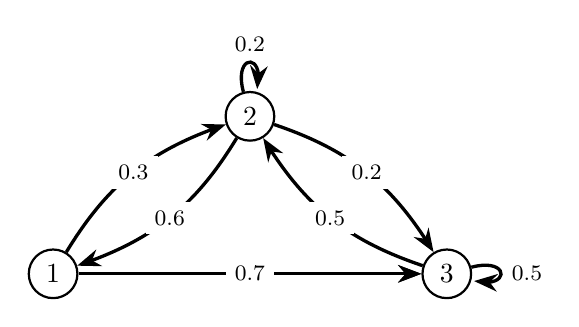
\begin{tikzpicture}
\begin{scope}[every node/.style={circle,thick,draw}]
    \node (A) at (0,0) {1};
    \node (B) at (2.5,2) {2};
    \node (C) at (5,0) {3};

    \end{scope}

\begin{scope}[>={Stealth[black]},
              every node/.style={fill=white,rectangle},
              every edge/.style={draw=black,very thick}]
    \path [->] (A) edge [bend left=20] node[pos=0.5] {\footnotesize{0.3}} (B);
    \path [->] (B) edge [bend left=20] node[pos=0.5] {\footnotesize{0.6}} (A);
    \path [->] (B) edge [bend left=20] node[pos=0.5] {\footnotesize{0.2}} (C);
    \path [->] (C) edge [bend left=20] node[pos=0.5] {\footnotesize{0.5}} (B);
    \path [->] (A) edge (C);
    \path [->] (A) edge node[pos=0.5] {\footnotesize{0.7}} (C);
    \path[<->] (C) edge [loop right] node {\footnotesize{0.5}} ();
    \path[<->] (B) edge [loop above] node {\footnotesize{0.2}} ();
    
    \end{scope}

\end{tikzpicture}
\end{center}


% \begin{equation} \label{eq8}
% \begin{split}
% N_{open1}^{i+1} &=  e^{-\Delta t / \tau_{open}}N_{open1}^{i} + \pr{1 - e^{-\Delta t P_{total}}}N_{closed}^{i} \\ 
% N_{open2}^{i+1} &= \pr{1 - e^{-\Delta t P_{total}}}N_{open2}^{i} + P_{P}\pr{1-e^{-\Delta t / \tau_{open}}}N_{open1}^{i} \\ 
% N_{inactive}^{i+1} &= e^{-\Delta t / \tau_{inact}}N_{inactive}^{i} + \pr{1-P_{P}}\pr{1-e^{-\Delta t / \tau_{open}}}N_{open1}^{i} + e^{-\Delta t P_{P}}N_{open2}^{i}\\
% N_{closed}^{i+1} &= e^{-\Delta t P_{total}}N_{closed}^{i} + \pr{1-e^{\Delta t / \tau_{inact}}}N_{inactive}^{i} \\
% \end{split}
% \end{equation}




\chapter{Neuron Modeling}

It would certainly be worth reviewing the electrophysiology contained in Part \textbf{\ref{sec:Physiology}} before trying this, unless you already have a strong understanding of biochemistry.  


\section{Hodgkin-Huxley} 

\subsection{The Main Form} The pair won the nobel prize for this model, which formed the basis of our understanding of action potentials. Beyond neurons, it was used in modeling pacemakers of the heart, and muscle cell depolarizations before better models existed.  The basis is simply KCL: 

\bigskip

\begin{equation} \label{hh1}
\begin{split}
C\dot{V} = I - I_{Na} - I_{K} - I_{Leak}
\end{split}
\end{equation}

\bigskip

Because the equations can be found in nearly any textbook\footnote{Izhikevich, \textit{Dynamical Systems Neuroscience}} or Wikipedia page, I will focus on some of the conceptual understanding I had issues with at first. The complete equation Hodgkin and Huxley arrived at is as follows: 

\bigskip

\begin{equation} \label{hh2}
\begin{split}
C\dot{V} = I - \bar{g}_{Na}m^3h(V - E_{Na}) - \bar{g}_{K}n^4(V - E_{K}) - \bar{g}_{L}(V - E_{L})
\end{split}
\end{equation}

\bigskip 

There are a few main points to make here. Firstly, this model considers only 3 currents. $Na$ and $K$ are self explanatory, but $Leak$ represents the small amount of current that will always occur in cells due to the many routes of charged particles passing through the membrane. It is restorative, in that it pushes the membrane potential back to the resting voltage.\newline

\subsection{Gating and Conductance} 

\label{sec:GatingandConductance}

The $\bar{g}$ represent the maximal conductance of these ions. Of course, you mak ask, ``\textit{shouldn't conductance be variable, depending on how many channels are open}?" Yes, which is what $m$, $h$, and $n$ are for! These three variables are effectively kinetic fits of the opening and closing dynamics of sodium and potassium channels. Again, I will not mention these equations explicitly as they can be found anywhere. Conceptually, there are three things to know:\newline

Firstly, $m$ is an activation curve for sodium, and the power to the 3rd represents that there are three activation gates. $h$ is an inactivation gate for sodium. Potassium has 4 activation gates, $n$, and no inactivation gate. Gating can be any number of things, for example, $h$ could be a conformtional change that occurs in the channel after it has been open for $0.1 ms$ that closes it again. Naturally, the gating for every channel will be different. Because the $Leak$ current is an ensemble of many channel types, it will not have "gating" per se.\newline

Secondly, $m$, $h$, and $n$ all are between 0 and 1 and represent the \textbf{proportion of channels open}. For instance, if $n = 1$, then 100\% of potassium channels will be open. This is why we multiply by the maximal conductance.\newline

Thirdly, $m$, $h$, and $n$ are dependent upon voltage, which affords them a time constant $\tau$. This is the conceptually most difficult part. The experimental explanation may be beneficial in understanding. Hodgkin and Huxley realized that these three gating variables will converge to different values depending on the voltage. This makes sense, because we know potassium channels are voltage gated, we would expect the gating variable $n$ to converge to around 1 as the voltage increases. But, the rate at which channels open and close is different. Therefore, their experiments were done to vary the voltage and determine how long it took the conductance of the channels to converge to some value. Does this make sense? In simplest terms: channels open and close at different rates, and that depends on the voltage.\newline

What is the implication of this? Again, look up the exact equations if you are interested. Otherwise, trust the following: $m$ has a time constant $\tau_m$ which is very small compared to $\tau_h$ and $\tau_n$. Meaning, sodium channels will open the fastest in response to a voltage increase, causing depolarization of the cell. After some delay, sodium channel inactivation ($h$) and potassium channel activation ($n$) will kick in, causing repolarization and then hyperpolarization. 

\subsubsection{These are all derivatives.}
One of the most difficult conceptual understandings I had was that $\dot{V}$, $m$, $h$, and $n$ are all rates that depend on different time constants, which take voltage as their input. So, the derivative of voltage depends on the derivative of $m$, $h$, and $n$, which depend on voltage. The cyclic nature of this makes it strange, but still doable. Use the general form of derivative, $x_{i+2} = x_{i+1} + (x_{i+1} - x_i)/t$, follow the math, and you will survive.

\section{Fitzhugh-Nagumo Reduction}

\subsection{Why would we simplify this system?} Reduction implies we are reducing the amount of variables. But why would we do this? The system is already incredibly generalized. We only consider two ion channels and are looking at a static neuron. How can we be accurate if we simplify this system any further?\newline

Let's start by doing a simple thought experiment regarding the previous model: 

\bigskip

\begin{center}

    $C\dot{V} = I - \bar{g}_{Na}m^3h(V - E_{Na}) - \bar{g}_{K}n^4(V - E_{K}) - \bar{g}_{L}(V - E_{L})$
    
\end{center}

\bigskip

As mentioned, $m$, $h$, and $n$ have their own time constants $\tau_{m,h,n}$. That means you'll need to do at least 6 calculations in order to determine $\dot{V}$, which, because it is a derivative, has its own time constant $\tau_v$. Thus, the whole equation is $4^{th}$ dimensional with respect to time and requires at least 7 or so calculations per time step. If you'd like to simulate an action potential for around 10ms with a time step of 0.01ms, that means you'll perform around 7,000 calculations. Which is not so bad!\newline 

However, let's say you want to attempt a propagating action potential. Many people would model this on an infinitely long neuron/wire, but for the sake of this thought experiment let's say you're just interested in a 1 cm neuron/wire for 10 ms. To account for this spatial consideration, you'll need to add in another term besides $I$ which receives current input from the previous segment of the neuron. So, this brings us up to at least 8,000 calculations.\newline

You'd probably want to divide up the neuron into segments on the order of 1 $\mu$m. This multiplies our 8,000 calculations by an additional 100,000, giving us 800,000,000 to worry about. Still, this is not horrendous. But, this considers a 1D wire. Neurons are 3D dimensional. We are already considering a system that is $4^{\mathrm{th}}$ dimensional with respect to time, and now we desire to consider $3^{\mathrm{rd}}$ dimensional with respect to space. Imagine trying to calculate the flux through a $1000 \times 1000 \times 1000$ resolution box (i.e., perhaps $\mu m^3$ with good resolution). The surface area of this box is thus $6\times 10^6$. Now extend this surface area to include the length of the wire and the area of the soma and dendrites, giving you thousands of millions of points to calculate per time iteration. And, we are still only considering two ion channels. Neurons have dozens and dozens of channels all with different gating kinetics. It does not consider things like lateral inhibition, birufcation, dendritic input, etc. I'll not bother telling you how many calculations we need to perform beyond this point---but it would be large. 

\subsection{How to Reduce} 

\textcolor{blue}{A note from future Jackson: I believe this section was written sometime in early 2023. After taking Mathematical Biology, I realize how stupidly simplified this is! It provides a good bit of conceptual understanding, but the actual path to creating the FHN model was much more complicated and elegant. FHN also provided the basis for many Dynamical Systems, extending far beyond neuroscience. It should be wholly respected.}\newline

What do we know about the time constants mentioned in the previous section? Roughly speaking, some are fast and some are slow. The upswing of an action potential is on a fast time constant, and the repolarization is on a slow time constant. We also know that the upswing portion is roughly a positive feedback loop, so as voltage increases, so should the derivative of voltage.\newline

This helps us arrive at least at the following: 

\begin{equation} \label{fn1}
\begin{split}
\dot{V} &= V \times f(x)
\end{split}
\end{equation}


Simply meaning that the derivative should scale with voltage in some way. We also know that there are at least two ``equilibrium points" in a neuron. Meaning, when the neuron is at rest, the $\dot{V}$ will be zero. And, when the neuron reaches the peak of the action potential, the same is true. This will allow us to immediately assume something interesting:

\begin{equation} \label{fn2}
\begin{split}
\dot{V} &= V(V - V_{rest})(V_{max} - V)
\end{split}
\end{equation}

We are already almost there. What we have just done is said that when either $V = V_{rest}$ or $V = V_{max}$, the $\dot{V}$ will not change. These are all on the aforementioned ``fast" time scale, and as this is representative of the activation of the action potential, it is effectively a simplification of the sodium channel dynamics. This is also extremely easy to measure experimentally.\newline

On our second time scale, the slow time scale, we have the inactivation/repolarization function. How will this look like? Just as with the first equation, we will want this curve to increase in magnitude with voltage. Because $n$ represented the potassium channel activation in the previous segment, we can use that as our repolarization function here. 

\begin{equation} \label{fn3}
\begin{split}
\dot{n} &= V - \gamma n
\end{split}
\end{equation}

What does this say? It says that our repolarization curve $\dot{n}$ will increase with respect to voltage. But, it will also decrease with respect to itself according to some scaling factor $\gamma$.\newline

Now we have reduced our function down to two dimensions and can combine terms: 
    
\begin{equation} \label{fn4}
\begin{split}
    \dot{V} &= V(V - V_{rest})(V - V_{max}) - n\\ 
    \dot{n} &= V - \gamma n\\
\end{split}
\end{equation}

But, we still want voltage to be affected by an injected current, so we can simply add this term back in. And it is also in this equation that we will add our spatial dependence to reach the following: 

\begin{equation} \label{fn5}
\begin{split}
    \dot{V} &= I_{app} + [V(V - V_{rest})(V - V_{max}) - n] +  D\frac{\partial V^2}{\partial x^2}\\
\end{split}
\end{equation}

$D$ is our spatial dependence, which represents the diffusion of charge around the neuron membrane. And that's it, for now! 

\subsubsection{Circuits digression.}
A lot of the original work done by Fitzhugh and Nagumo used circuit equivalents in order to model neurons. One such example is as follows\footnote{This circuit is adapted from {\textit{Mathematical Physiology}}, by James Keener \& James Sneyd (1998).}:

\begin{center}
 \begin{circuitikz} 
 \draw
    (0, 0) node[op amp,yscale=-1] (opamp) {}
    (opamp.+) to[short] ++(-1,0) 
    to[C] ++(0,1.5)
    (opamp.+) to[short] ++(-1,0)
    to[R] ++(0,-1.5)
    to ++(0,0) node[ground]{}
    (opamp.-) to[short] ++(0,-1) coordinate (leftS)
    to[short] (leftS -| opamp.out)
    to[short] (opamp.out)
    to[R] ++(0,2)
    (-4,2) -- (2,2)
    (-4,2) to[C] (-4,0)
    to ++(0,0) node[ground]{}
    (3.5, 0.5) node[op amp,yscale=-1] (opamp) {}
    (opamp.+) to[short] ++(-0.5,0) 
    to[short] ++(0,1)
    (opamp.-) to[short] ++(-0.5,0) 
    to[short] ++(0,-1)
    to[R] ++(0,-2)
    to ++(0,0) node[ground]{}
    (1.81,-1) to[R] (4.7,-1)
    to[short] (opamp.out)
    to[short] ++(0,1.5)
    to[R] ++(-3,0)
;
\end{circuitikz}

\end{center}

The rightward opamp functions as a Schmitt Trigger, and the entire thing is effectively an opamp oscillator with a second opamp in the middle. The purpose is to simulate an excitable system, like a neuron that is continually firing. Excitable systems systems are those that fire and have some refractory period before firing again (for example forest fires, or even your toilet).


\section{Diffusion}

 Note that in the coming sections, $[f]$ is used to describe the concentration of some molecule $f$. But, this principal can be applied to anything, including the spreading of voltage across some surface. 

 \subsection{Diffusion Equation Derivation}

So, let's consider some particle that adheres to the arbitrary function $f(x)$, and has some probability density function of $\Psi(x,t)$ and experiences some noise of $W$. We can know that, regarding $W$:

\begin{equation}
\begin{split}
    dW = 0 \\
    dW^2 = dt
\end{split}
\end{equation}

By the It$\overline{\mathrm{o}}$ lemma. And where $dx = \alpha dW$, where $\alpha$ is some function of $k_BT$ and the mobility coefficient, $M$, of the particle. We can say for an ensemble of particles that: 

\begin{equation}
\begin{split}
    \langle f(x) \rangle(t) = \int \Psi(x,t) f(x) dx
\end{split}
\end{equation}

If we are interested in the change of $f(x)$ over $dx$, we consider: 

\begin{equation}
\begin{split}
    df = f[x + dx] - f[x] 
\end{split}
\end{equation}

And we Taylor Expand around $df$ as: 

\begin{equation}
\begin{split}
    df & = f'\alpha dW + \frac{1}{2}f''\alpha^2 dW^2 + \mathcal{O}dW^3 \\
    df & = f'\alpha dW + \frac{1}{2}f''\alpha^2 dt + \mathcal{O}dtdW
\end{split}
\end{equation}

If we average over the ensemble, we get: 

\begin{equation}
\begin{split}
    \frac{d\langle f \rangle}{dt} & = \frac{1}{2}\langle f'' \rangle \alpha^2 
\end{split}
\end{equation}

This can be solved as: 

\begin{equation}
\begin{split}
    \frac{\partial \Psi}{\partial t}f & = \frac{1}{2} \frac{\partial^2 \Psi}{\partial x^2}f \alpha^2
\end{split}
\end{equation}

And, because $f$ never meant anything anyway, we are saying: 

\begin{equation}
\begin{split} \label{sec:diffequation}
    \frac{\partial \Psi}{\partial t} & = D_c \frac{\partial^2 \Psi}{\partial x^2} 
\end{split}
\end{equation}


\subsubsection{Another approach.}

Let's consider beginning this equation with the Master equation, which describes the probability (still using $\Psi$) of being at position $r$ at time $t + \Delta t$ for one dimension as: 

\begin{equation}
\begin{split}
    \Psi(r,t + \Delta t) = \Phi\Psi(r - \Vec{e_i},t) + (1 - \Phi)\Psi(r + \Vec{e_i},t)
\end{split}
\end{equation}

Where $\Phi$ is the probability of moving left by a distance of $\Vec{e}_i$ along your 1-dimensional lattice. In other words, $\Vec{e}_i$ is the discrete length that you can travel along this lattice. Do you hate this notation? Me as well.\newline

Let us know try to find the solution to this by Taylor expansion: 

\begin{equation}
\begin{split}
    \Psi + \Delta t\frac{\partial \Psi}{\partial t} &= \Phi\pr{\Psi - \Vec{e_i}\Psi' + \frac{\Vec{e_i}^2}{2}\Psi''} + (1 - \Phi)\pr{\Psi + \Vec{e_i}\Psi' + \frac{\Vec{e_i}^2}{2}\Psi''} \\
    \Delta t\frac{\partial \Psi}{\partial t} &= -2\Phi\Vec{e_i}\Psi' + \Vec{e_i}\Psi' + \frac{\Vec{e_i}^2}{2}\Psi'' \\
    \frac{\partial \Psi}{\partial t} &= \frac{\Vec{e_i}(1-2\Phi)}{\Delta t}\Psi' + \frac{\Vec{e_i}^2}{2\Delta t}\Psi'' \\
\end{split}
\end{equation}

Which we can simplify to: 

\begin{equation}
\begin{split}
    \frac{\partial \Psi}{\partial t} &= \frac{\Vec{e_i}(1-2\Phi)}{\Delta t}\frac{\partial \Psi}{\partial x} + D_c\frac{\partial^2 \Psi}{\partial x^2} \\
\end{split}
\end{equation}

We could assign the value of $\Vec{e_i}(1-2\Phi) /\Delta t$ to be some constant. But, in general, $\Phi = 0.5$, signifying an equal probability of moving left or right, so this entire term is deleted, giving us the same as we got for equation \textbf{\ref{sec:diffequation}}. 



\subsection{Forward Euler's} Diffusion is accomplished using some diffusion coefficient ($D_c$) multiplied by some measure of the proportion in one compartment verses another (often $\partial^2 [f]/\partial x^2)$. $D_c$ can be tuned however desired. The important bit is the second derivative of $[f]$ with respect to space. This can be done using the general form of a second derivative, as written below: 

\begin{equation} \label{diff1}
\begin{split}
f'' = \frac{f_{x + 1} - 2f_x + f_{x - 1}}{x^2}
\end{split}
\end{equation}

\bigskip

One may wonder how one would solve for an edge case, as the general form of a second derivative requires three data points. There are some nuances, but in general the solution is simply the first derivative of the non-edge side. That is, since the second derivative is the difference in derivatives, that leaves simply the derivative of one side minus zero. This is like applying a closed end to your surface. You can ponder how to solve for an open end, if that ever arises.\newline

This method has some slight issues in which the $[f]$ can occasionally go negative. The way in which this occurs is stated below (note that now $[f]$ is used instead of $f$ to signify concentration at a value $x$ and time $t$). We can first describe a simplified version of the problem:

\begin{equation} \label{diff2}
\begin{split}
[f]_i & = f_0\exp(-mt) \\
\frac{d[f]}{dt} & = \frac{[f]_{i+1} - [f]_{i}}{\Delta t} = -m[f]_i \\
[f]_{i+1} & = (1-m\Delta t)[f]_i = [f]_i - m\Delta t [f]_i \\
[f]_{i} & = (1-m\Delta t)[f]_{i-1} = (1-m\Delta t)^2[f]_{i-2} \\
[f]_{i} & = (1-m\Delta t)^i[f]_{0} \\
\end{split}
\end{equation}

You can see easily, from this, that if $\Delta t$ is too big, you will abandon the characteristic decay you'd expect from $f_0\exp(-mt)$, and instead get some diverging oscillatory function. How this applies to our interest in diffusion is described below: 

\begin{equation} \label{diff3}
\begin{split}
\frac{[f]^{t+1}_{x} - [f]^{t}_{x}}{\Delta t} &= \frac{[f]^{t}_{x+1} - 2[f]^{t}_x + [f]^{t}_{x - 1}}{x^2}\\
[f]^{t+1}_{x} - [f]^{t}_{x} &= \frac{\Delta t}{x^2} \pr{[f]^{t}_{x+1} - 2[f]^{t}_x + [f]^{t}_{x - 1}} \\
[f]^{t+1}_{x} &= \frac{\Delta t}{x^2} [f]^{t}_{x+1} + \pr{1 - 2\frac{\Delta t}{x^2}}[f]^{t}_x + \frac{\Delta t}{x^2}[f]^{t}_{x - 1} \\
\end{split}
\end{equation}

Therefore, if we want to ensure that the concentration is always positive, we are constrained by: 

\begin{equation} \label{diff4}
\begin{split}
1 - 2\frac{\Delta t}{x^2} & = 0\\
\Delta t & < \frac{x^2}{2}\\
\end{split}
\end{equation}

The relevance of this being that if one were interested in modeling on a very small $\Delta x$, then one would have to use a $\Delta t$ that is not physiological, and thus waste a great deal of computing power in doing so. This can be avoided explicitly using some other methods, discussed next. 

\subsection{Backward Euler's} This form serves to solve the time-scale dilemma by swapping $[f]_{x+1}$, and can be used with any $\Delta t$. Let us consider the same example from above: 

\begin{equation} \label{diff5}
\begin{split}
[f]_i & = f_0\exp(-mt) \\
\frac{d[f]}{dt} & = \frac{[f]_{i+1} - [f]_{i}}{\Delta t} = -m[f]_{i+1} \\
[f]_{i+1} - [f]_{i} & = -m\Delta t[f]_{i+1} \\
[f]_{i+1} & = \frac{1}{1+m\Delta t}[f]_{i} \\
\end{split}
\end{equation}

Naturally, there is no longer a concern of the size of $\Delta t$. Though, one immediate concern is the difficulty of solving your equation for $[f]_{i+1}$. Getting back to the diffusion interest, we now have:

\begin{equation} \label{diff6}
\begin{split}
\frac{[f]^{t+1}_{x} - [f]^{t}_{x}}{\Delta t} &= \frac{[f]^{t+1}_{x+1} - 2[f]^{t+1}_x + [f]^{t+1}_{x - 1}}{x^2}\\
[f]^{t+1}_{x} - [f]^{t}_{x} &= \frac{\Delta t}{x^2} \pr{[f]^{t+1}_{x+1} - 2[f]^{t}_x + [f]^{t-1}_{x - 1}} \\
\end{split}
\end{equation}


Which simply replaces the previous $[f]^{t}_{x}$ with $[f]^{t+1}_{x}$. This leaves us with three unknowns (those being $[f]^{t+1}$ at $x-1,x,x+1$). We must use linear algebra to solve by first rewriting the left and right side as vectors and a matrix in the following way: 

\begin{align}
\vec{[f]}^{t+1} &= \begin{bmatrix}
        [f]^{t+1}_{0} \\
        [f]^{t+1}_{1} \\
        \vdots \\
        [f]^{t+1}_{x}
\end{bmatrix}
; \vec{[f]}^{t} = \begin{bmatrix}
        [f]^{t}_{0} \\
        [f]^{t}_{1} \\
        \vdots \\
        [f]^{t}_{x}
\end{bmatrix}
\end{align}

and 
\begin{align}
\mathrm{A} = \frac{\Delta t}{x^2}
\begin{bmatrix} %%%%%%%%%%%%%%
\dots       &   \dots       & \dots     &   \dots    &   \dots   \\
1           &   -2          & 1         &            &   \vdots    \\
\vdots      &   1           & -2        &   1        &   \vdots   \\   
\vdots      &               & 1         &   -2       &   1    \\
\dots       &   \dots       & \dots     &   \dots    &   \dots    \\
\end{bmatrix}
\end{align}

The corners $1,1$ and $x,x$ were intentionally omitted, as what one desires to do with this is dependent on how they would prefer to treat their edges. As described before in the \textit{Forward Euler's} method, one can use instead of the $(1,-2,1)$ pattern, simply $(\varnothing,-1,1)$ pattern, which signifies a closed edge. Therefore, together now we get: 

\begin{equation} \label{diff7}
\begin{split}
\vec{[f]}^{t+1} - \vec{[f]}^{t} & = \mathrm{A} \vec{[f]}^{t+1} \\
\mathrm{I}\vec{[f]}^{t+1} - \mathrm{A}\vec{[f]}^{t+1} & = \vec{[f]}^{t} \\
\vec{[f]}^{t+1} & = (\mathrm{I} - \mathrm{A})^{-1}\vec{[f]}^{t}
\end{split}
\end{equation}

Where I is the identity matrix. 

\subsubsection{Remarks.} 
Foward Euler's is explicit, and will be preferred whenever the differential equations are non-stiff\footnote{On approximately the same time scale.}. It is the more accurate of the two methods, and can be less computationally intensive if your decay rates are all slow. Backward Euler's is implicit, and can not be used to solve everything, but is doable in most cases. The extra computation required to solve the system of equations more than makes up for potential limitations in your $\Delta t$. 

\subsubsection{Ramblings.} 
I have this constant wonder if this method can be used to model the spread of voltage over a resistor lattice, by perfecting the $D_c$ value. I am presuming it would work for a sufficiently large lattice, perhaps $100 \times 100$. This would be a good exercise to do sometime in the future. 



\chapter{Math in Electronics}

\section{Modeling Circuits}
\label{Modeling Circuits}

The idea of this algorithm comes from\footnote{\url{https://lpsa.swarthmore.edu/Systems/Electrical/mna/MNA3.html}} and is an expansion of what was discussed earlier in section \textbf{\ref{sec:resistorlattice}}. Not by coincidence, both of the examples in the earlier section had symmetric matrices. The general way to extract equations from a circuit is in the following pattern:   

\begin{align}
\begin{bmatrix} 
\mathrm{G} &   \V \\
\V^T   &   \mathrm{Z}  \\
\end{bmatrix}
\end{align}

G is essentially the way nodes are connected by resistors (represented as conductances). The diagonal represents the total number of resistors connected to a diagonal, and the other bits represents how nodes are connected by resistors. I will use the example provided in the footnote directly to illustrate: 

\begin{center}
\begin{circuitikz}[american]
\draw 

(-3,-1) to [battery,l_=$V_{s1}$] (-5,-1)
(-5,-1) to [R,l_=$R_1$] (-5,-3)
(-5,-3) -- (-3,-3)

(-1,-1) to [battery,l=$V_{s2}$] (-1,-3)
(-1,-1) to [R,l_=$R_2$] (-3,-1)
(-3,-1) to [R,l_=$R_3$] (-3,-3)
(-3,-1) to [short, *-] (-3,-1)
(-1,-1) to [short, *-] (-1,-1)
(-3,-3) to [short, *-] (-3,-3)
(-5,-0.55) node {$V_1$}
(-3,-0.55) node {$V_2$}
(-1,-0.55) node {$V_3$}
(-2.7,-2.7) node {$V_4$}
(-5,-1) to [short, *-] (-5,-1)
(-1,-3) -- (-3,-3)
to ++(0,0) node[ground]{};

\end{circuitikz}
\end{center}

There are 4 nodes, but as mentioned before, Node 4 is grounded, a reference, and thus not included in our calculations. This will mean our matrix G must be $n \times n$, where $n$ is $N - 1$. Node 1 is connected only to $R_1$, resolving the $(0,0)$\footnote{You are a computer scientist in addition to a mathematician, so of course our matricies must be 0 indexed.} position of the matrix to be $G_1$. Node 2 is connected to $R_2$ and $R_3$, giving us $(1,1) = G_2 + G_3$. Node 3 to only $R_3$, giving us $(2,2) = G_3$. Node 2 and Node 3 are connected via $R_2$, meaning the $1,2$ and $2,1$ positions will have a $G_2$, though notably, it will be $-G_2$:

\begin{align}
\mathrm{G} = 
\begin{bmatrix} 
G_1 & 0 & 0 \\
0 & G_2 + G_3 & -G_2 \\
0 & -G_2 & G_2 \\
\end{bmatrix}
\end{align}

There are two voltage sources ($V = 2$), and 3 nodes, meaning the matrix must be $n \times m$, where $n = N-1$ and $m = V$. You fill the matrix as if the positive terminal of the $j^{\mathrm{th}}$ voltage source is connected to the $i^{\mathrm{th}}$ node, point $(i,j) = 1$, or $(i,j) = -1$ for the negative terminal. So for the above, since the negative terminal of $V_{s1}$ is connected to Node 1, $(0,0) = -1$, and as the positive terminal connects to Node 2, $(1,0) = 1$. Lastly, as Node 3 connects to the positive terminal of $V_{s1}$, $(2,1) = 1$. 
\begin{multicols}{2}
\begin{align}
\mathrm{V} = 
\begin{bmatrix} 
-1 & 0 \\
1 & 0  \\
0 & 1  \\
\end{bmatrix}
\end{align}

\begin{align}
\mathrm{V}^T = 
\begin{bmatrix} 
-1 & 1 & 0 \\
0 & 0  & 1 \\
\end{bmatrix}
\end{align}
\end{multicols}

And lastly, Z for zero is an $n \times n$ matrix of zeros where $n = V$:

\begin{align}
\mathrm{V}^T = 
\begin{bmatrix} 
0 & 0  \\
0 & 0   \\
\end{bmatrix}
\end{align}

Giving us an $\mathrm{A}x = \mathrm{B}$ of: 

\begin{align}
\begin{bmatrix} 
G_1 & 0 & 0 & -1 & 0 \\
0 & G_2 + G_3 & -G_2 & 1 & 0  \\
0 & -G_2 & G_2 & 0 & 1  \\
-1 & 1 & 0 & 0 & 0  \\
0 & 0  & 1 & 0 & 0  \\
\end{bmatrix}
\begin{bmatrix} 
V_1 \\
V_2  \\
V_3  \\
I_1  \\
I_3 \\
\end{bmatrix}
=
\begin{bmatrix} 
0 \\
0  \\
0  \\
V_{s1}  \\
V_{s2} \\
\end{bmatrix}
\end{align}

You may, rightfully, say ``\textit{Uh, who cares?}," since we already know that each row corresponds to a different equation. Well, there are a few reasons. Firstly, doing this algorithmically allows us to avoid accidentally underdetermining our matrix using the ol' eye-balling it technique. More importantly, though, the algorithmic approach allows us to solve this via code. Once I can write a bit more neatly, I'll likely upload some snippets here. 


\subsection{Error Correction Codes, Hamming}

We know digital files are stored as 1s and 0s\footnote{\url{https://www.youtube.com/watch?v=X8jsijhllIA&ab_channel=3Blue1Brown}}. However, there must be a mode of corruption-prevention, lest any sort of damage, where it be digital (a 1 misread and stored as a 0) or physical (the scratching of a CD), would lead to loss of signal. A simple way to do this would simply be to store additional copies of every file, and allow your computer to compare the copies and select the proper result. Let us consider Hamming codes, the old-style technique for error correction.\newline

Long ago, a so-called method of parity check was invented. Simply put, if you have an $n \times n$ array of binary numbers, a single additional bit was allocated to determine if the number of 1s is even or odd. Therefore, you can allocate this parity position for an $n \times n$ array such that the probability of error is unlikely to occur twice. This of course allows you to detect the existence of an error, but not its location or the ability to correct it.\newline

First, consider an array of bits, say $3\times 3$. To exactly identify any errors in said bits, you might expect you'd need a 9-bit copy. However, imagine instead that you use a Sudoku-style arrangement, where 6 bits are stores on the edges of this array and determine the sum of the indices (summing the bits: $000 = 0$, $010 = 1$, $110 = 0$, etc.). Now, you can certainly identify an error, such that if you have a row $000 = 1$, you can know one of the bits has flipped. By comparing with the other sums, you can identify which of the three.\newline

Now suppose that rather than applying these checks to the edges, you instead apply parity checks to certain subsets of a larger $n \times n$ matrix. How can we apply parity checks in clever ways such that they minimize memory and maximize our ability to check for errors? Consider the bits in the matrix below, where bolded bits are parity bits. 

\begin{center}
\begin{multicols}{3}

Correct: \medskip

    \begin{tabular}{c|c|c|c}
         $x$ &  \textbf{1} & \textbf{1} & 0 \\
         \textbf{1} &  1 & 0 & 0\\
         \textbf{0} & 0 & 1 & 1\\
         1 & 0 & 0 & 1
    \end{tabular}


Incorrect: \medskip

    \begin{tabular}{c|c|c|c}
         $x$ &  \textbf{1} & \textcolor{cyan}{\textbf{0}} & 0 \\
         \textcolor{cyan}{\textbf{0}} &  1 & 0 & 0\\
         \textcolor{cyan}{\textbf{1}} & 0 & 1 & 1\\
         1 & 0 & \textcolor{red}{1} & 1
    \end{tabular}

Incorrect: \medskip

    \begin{tabular}{c|c|c|c}
         $x$ &  \textbf{1} & \textcolor{red}{\textbf{1}} & 0 \\
         \textbf{1} &  1 & 0 & 0\\
         \textbf{0} & 0 & 1 & 1\\
         1 & 0 & 0 & 1
    \end{tabular}

\end{multicols}
\end{center}

Parity bit at position $(1,2)$ ($P_{1,2}$) can check for parity in columns 2 and 4---which I will write as $(:,2)$ and $(:,4)$ now as in Python notation. $P_{1,3}$ can check for parity in $(:,3)$ and $(:,4)$. Therefore, you can immediately localize a single error to its correct column. That is, if $P_{1,2}$ and $P_{1,3}$ are both incorrect, you can know immediately that the error must be in column 4. Similarly, $P_{2,1}$ can check error in $(2,:)$ and $(4,:)$, and $P_{3,1}$ can check for error in $(3,:)$ and $(4,:)$. You can see clearly how the error can be localized to a single bit from the examples above. Naturally, though, there is complete breakdown when there is more than one error. You may ask: what if a parity bit gets corrupted? Consider the third column---only the parity bit itself changes. No other parities recognize an error. Therefore, the computer can localize the error to this bit, once again.\newline

Position 0 is intentionally left as an $x$. No altered parity bits suggests either that there are no errors, or that the error is in position 0. To avoid questions with this 0th position, we can either discard it, or allocate it as a second tier of parity. One such way to do so will be to use it as a whole-number parity. That is, if this bit flips once, you can know there was one error. If it flips twice, you can know there are at least two errors. One would normally call the example above a $(15,11)$ Hamming code, and adding the 0th block is called an extended Hamming code. \newline

Now the question is, how do we scale? First, ask yourself: how many binary searches are required to fully parse a $2^n - 1$ binary number? Well, just now we saw that a 16-bit number requires $4$ parity bits to be allocated. Therefore, a $2^8 - 1 = 256$ bit number requires 8 parity bits. 




\chapter{Fluid Mechanics and Cell Motility}

\textcolor{red}{This either needs complete removal or a serious overhaul---I was not as diligent as I hoped I would be with fleshing out this section.}

\section{Introduction}

The life of small things is hard. Brownian motion reorients E. coli a full 90$^\circ$ approximately once per second. The objects which they are trying to chase after and eat, too, undergo Brownian motion. A good question to ask yourself, then, is what do they do to make it worth it?

\section{Cell Motility}

I have an idea. I'm wondering if you can use cell motility models, with a bit of adaptation, and use it to model growth cone motility. I.e., model an ensemble of neurons after injury. The motivation being that the architecture of the neurons after injury is quite important to recovery. This idea, sprouting, is explored in-depth throughout this work, such as in a discussed Courtine review. Similarly, the movement of axons on a single cell level is naturally a form of cell motility. \newline

There have been a number of papers that have gathered the 3D structure of axons after injury---so it is not impossible to verify models\footnote{\url{https://www.sciencedirect.com/science/article/pii/S0896627321007753?via\%3Dihub}}$^,$\footnote{\url{https://www.sciencedirect.com/science/article/pii/S2211124720308883?via\%3Dihub}}. 


\section{Fluid Mechanics}

There are two main open questions in the field of fluid mechanics. First, Newton's equations have been used for centuries and, in large part, model the world very well. However, we still haven't determined if these work completely, in all cases. Another open question is the origin of turbulence. Broadly speaking, we can define fluids as something that can be deformed, are continuous, and have no memory of its previous position. Complex fluids, like toothpaste, exhibit both fluid-like behaviors, but also retain their shape when left alone. \newline

Knudsen number is used to define how continuous a fluid is: 
\begin{equation} \label{knum}
\begin{split}
K_N = \frac{\lambda}{L}
\end{split}
\end{equation}

Knowing a system is continuous allows us to define dynamic, average quantities like $\rho(x;t), p(x;t), \mathbf{u}(x;t)$. Our pressure value, $p(x;t)$, is useful in defining the resistance of a fluid to force. Pressure is isotropic, meaning it is independent of direction. Defining the velocity, $\mathbf{u}(x;t)$, may be done by quantizing some small segment of the fluid and following its trajectory. This is the Lagrangian description. The trajectory that your quantized box follows is called the \textit{pathline}. Alternatively, the Eulerian description treats the fluid as an ensemble, defining $\mathbf{u}$ everywhere and producing a vector-field like array of streamlines. Conversion between the Lagrangian and Eulerian descriptions is:\newline

\begin{equation} \label{LtoE}
\begin{split}
\frac{Df}{Dt} = \frac{\partial f}{\partial t} + \mathbf{u}\cdot f
\end{split}
\end{equation}

You can define movement of a fluid with three fundamental flows: translation, rotation (solid body), and extension. Translation and rotation both do not cause any deformation. The streamlines simply move in unison in some direction. Extension causes deformation, and have hyperbolic streamlines. A microfluidic chamber, in which 4 channels come together in a cross, is an example of extension flow. At the intersection, components will be stretched. Deformation like this will lead to friction.\newline

\subsubsection{The Reynolds Number.}

A large part of this section will come from\footnote{\url{https://www.cambridge.org/us/universitypress/subjects/mathematics/fluid-dynamics-and-solid-mechanics/fluid-dynamics-cell-motility?format=HB&isbn=9781107174658}} and\footnote{\url{https://pubs.aip.org/aapt/ajp/article-abstract/45/1/3/1043148/Life-at-low-Reynolds-number?redirectedFrom=fulltext}}.\newline

The Reynolds number, $R_e$, described the flow of a fluid and is used to characterize it as turbulent or laminar. Such turbulent or laminar flow is interesting and important in biology. For example, flow in the circulatory system is typically turbulent (unless we are discussing the capillaries). Areas of high turbulence are known to accumulate plaques more frequently. It is calculated as: 

\nopagebreak

\begin{equation} \label{Redefinition}
\begin{split}
R_e & = \frac{\rho LU}{\eta}
\end{split}
\end{equation}

\begin{equation} \label{Redefinition2}
\begin{split}
R_{e\omega} & = \frac{\rho L^2\omega}{\eta}
\end{split}
\end{equation}

\nopagebreak

Where $\rho$ described the density of the fluid, $L$ describes the characteristic length, $U$ describes the flow speed, and $\mu$ describes the fluid's viscosity. It is common to see these variables interchanged with others, such as describing $U$ as $v$, or $\eta$ as $\mu$, or others. Another common thing you may see is the replacement of $\rho / \eta$ with a different constant called the \textit{kinematic viscosity}, usually represented by $\nu$. \newline

The Reynolds number can be interpreted as a ratio of the inertial force to the viscous force. An $R_e$ less than $10^3$ is considered to be viscous dominated and laminar. An $R_e$ greater than $10^4$ is considered inertia dominated and turbulent. A more apt description may be that the viscous nature of the fluid holds significantly less weight for something at a high $R_e$---meaning that a blue whale's motion, which swims at an $R_e$ of around $10^7$, is dictated nearly purely by inertia, as you would expect. In microbiology, $R_e$ is $<< 1$, making it highly viscosity dependent.\newline

A nice equation you can find is the following: 

\begin{equation} \label{tow}
\begin{split}
\frac{\mu^2}{\rho} = F_{tow}
\end{split}
\end{equation}

$F_{tow}$ is the force required to ``tow" an object in some liquid when $R_e = 1$. That is, any object with $R_e = 1$ can be towed by this force. The purpose of this is to demonstrate that small $R_e$ is correlated to small forces. Another interpretation of $R_e$ is that if you have an object, like a micro organism, with a very small $R_e$, you could push it with all your might, and nearly the instant you stop pushing, it will immediately halt. This is, again, because it is completely inertia-independent.\newline

Swimming itself is a cyclic process, usually described as $n$ cycles. Reciprocal swimming is when one's motion is equal in either the forward or reverse direction, and where one ends up in the same state at the end of the cycle. Interestingly, at high $R_e$ this cycle of swimming is acceptable. The example described in \textit{Life at Low $R_e$} is a clam who opens its mouth to move and then closes it, shunting it forward and is carried by momentum. Of course, such momentum does not help at low $R_e$, so a swimmer must have multiple, non-reciprocal movements. 

\subsubsection{Lizard Digression.}

A neat question you can ask is how exactly a large animal, like a lizard, are able to run on water? To do this, we'll make a number of huge simplifications. First, let's say the lizard's foot deflects / indents the water in an approximately cube-like manner with a length $R$. The density of the fluid is what we'll call $\rho_f$. The speed that they're running we'll call $v$, and the frequency of their steps to be $\omega$. The force generated by stepping, also called the Shoke force, is due to the inertia of the fluid, and is summarized as: 

\begin{equation} \label{lizard1}
\begin{split}
F_{up} \approx R^3\rho_f v\omega
\end{split}
\end{equation}

The lizard is fighting the force of gravity pulling it down. If we take the lizard to be approximately cube like, with dimension $L$ and density $\rho_l$, then: 

\begin{equation} \label{lizard2}
\begin{split}
F_{down} &\approx L^3\rho_l g \\
R^3\rho_f v\omega &\geq L^3\rho_l g
\end{split}
\end{equation}

To simplify further, let's assume $R \approx L$, and that $\omega \approx v / L$. Now we can simplify to: 

\begin{equation} \label{lizard2}
\begin{split}
\rho_f \frac{v^2}{L} &\geq \rho_l g \\
v &\geq \pr{\frac{\rho_l}{\rho_f} gL}^{\frac{1}{2}}
\end{split}
\end{equation}

For the sake of not thinking too hard, you can intuit that body's have physiological limits. Perhaps theoretically, an elephant can run on water if it moves its legs fast enough. However, you can probably see that this isn't feasible; muscles have limits. Let's say the physiological constraint conforms to the following equation, where $K$ is a constant describing muscle output: 

\begin{equation} \label{lizard3}
\begin{split}
F v \leq \rho_l L^3 K \\
R^3\rho_f v^2\omega \leq \rho_l L^3 K \\
v \leq \pr{\frac{\rho_l}{\rho_f} L K}^{\frac{1}{3}} \\
\end{split}
\end{equation}

Therefore, the result you'll see is that to run on water, you are constrained between equation (\ref{lizard2}) and equation (\ref{lizard3}). At some point the result of (\ref{lizard2}) exceeds that of (\ref{lizard3}), making is so the burden of running on water exceeds physiological limits. This example wasn't explained in significant depth, and we made some grand simplifications, but the central theme is the ability to map the real, moving world onto equations and make some statements about what is possible. 


\subsection{Conservation of Mass}

Let's discuss a fluid at point $x$ and time $t$. Its velocity is $\mathbf{u}(x;t)$, and its density $\rho(x;t)$. If we are interested in some space, $\omega$, we can determine the mass of fluid in this space by: 

\begin{equation} \label{phenom1}
\begin{split}
\int_\omega \rho(x;t)d\omega
\end{split}
\end{equation}

If we are interested in the rate of change of fluid in our space $\omega$, we can determine it by:

\begin{equation} \label{phenom1}
\begin{split}
\int_\omega
\frac{\partial}{\partial t}\rho(x;t)d\omega
\end{split}
\end{equation}

Knowing that any change in mass of the fluid is due only to fluid flowing in and out of our space $\omega$, we can rewrite this integral in terms of fluid passing the space's boundaries, which we'll call $S$, and let's define a vector normal to this space as $\Vec{n}$. In other terms: 

\begin{equation} \label{phenom1}
\begin{split}
-\int_{S,\partial\omega}
\rho \mathbf{u} \cdot \Vec{n}dS = \int_\omega \nabla x \cdot [\rho \mathbf{u}]d\omega
\end{split}
\end{equation}


The conversion between the two is a result of Gauss' theorem. This also means that, because $\omega$ is arbitrary: 

\begin{equation} \label{phenom1}
\begin{split}
\frac{\partial}{\partial t}\rho(x;t) = -\nabla x\cdot [\rho(x;t)\mathbf{u}(x;t)]
\end{split}
\end{equation}

This is like saying the total change in density is equal to the change in density and velocity at all points $x$. Which we can rewrite in a way that is clearer, demonstrating mass is conserved: 


\begin{equation} \label{phenom1}
\begin{split}
\frac{\partial \rho}{\partial t} + \nabla \cdot (\rho \mathbf{u}) = 0
\end{split}
\end{equation}

Where $\partial \rho / \partial t$ is the change in density and $\nabla \cdot (\rho \mathbf{u})$ is the advection term. For an incompressible fluid, where your density is fixed, you are left with:

\begin{equation} \label{phenom1}
\begin{split}
 \nabla \cdot \mathbf{u} = 0
\end{split}
\end{equation}

This, of course, is the first equation in the Navier-Stokes equations, discussed in section \textbf{\ref{sec:imstoked}}.\newline

\subsection{Stress Tensor}

Conservation of momentum can be solved using the forces applied to the system. This includes body forces ($\mathbf{F}(x;t)\delta V$ for some volume $\delta V$) and forces applied to a segment of the surface ($\tau(x;t)\delta S$ for some surface $\Vec{n}\delta S$).\newline 

Body forces scale with $\mathcal{O} (\mathbf{F}L^3)$, and the canonical example is gravity. Forces applied to the surface include pressure, which scales with $\mathcal{O} (\mathbf{F}L^2)$. The force of friction (or viscosity), just as the friction of two solids, comes in two components: the normal force and the force which opposes movement laterally. \newline

To think about this, consider some arbitrary object with a face. Regardless of the face, it has some normal vector $\Vec{n}$, and let's say this surface has an area $A$. As mentioned before, body forces scale with $\mathcal{O} (\mathbf{F}L^3)$, while surface with $\mathcal{O} (\mathbf{F}L^2)$. This means that when $\lim_{V\to 0}$, body forces and surface forces must be equal. So let's think of $\tau$ as:

\begin{equation} \label{phenom1}
\begin{split}
 \tau(x;t) = \lim_{A\to 0}\frac{F}{A}
\end{split}
\end{equation}

Let's first think of a cube whose faces are aligned with basis vectors $\{\Vec{e_1}, \Vec{e_2}, \Vec{e_3}\}$. All traction vectors can be summarized using these components such that if we have vector $\tau$ acting in the direction $e_3$, we can describe it as:

\begin{equation} \label{phenom1}
\begin{split}
 \tau_{e_3} &= \sigma_{3,1}e_1 + \sigma_{3,2}e_2 + \sigma_{3,3}e_3\\
\tau_{i} &= \sigma_{i,j}e_j
\end{split}
\end{equation}

This works nicely and succinctly when we are discussing a vector $\tau$ in the direction of a basis vector. Cauchy describes a more general case for some arbitrary tetrahedron. Forces applied to three of the faces on the tetrahedron can be described using $\{\sigma_{i,1}, \sigma_{i,2}, \sigma_{i,3}\}$, but the fourth face is misaligned with the bases. The 4$^\mathrm{th}$ face of the tetrahedron has the normal vector $\Vec{n}$, which can be defined as $\Vec{n} = \Vec{n_1}e_1 + \Vec{n_2}e_1 + \Vec{n_3}e_1$. A force acting on this face, $\tau$ is not aligned with any basis vector, but we can cheat by splitting $\tau$ into its components, $\tau = \tau_{n_1} + \tau_{n_2}+ \tau_{n_3}$.\newline

I'm going to yada-yada through the proof a little bit, but the gist is that if you take Newton's laws and describe them for each normal, you get something along the lines of: 

\begin{equation} \label{phenom1}
\begin{split}
\sum \mathbf{F_{e_1}} = -\sigma_{1,1}n_1 - \sigma_{2,1}n_2 - \sigma_{3,1}n_3 + \tau_{n_1} + mg = ma
\end{split}
\end{equation}

Since, as mentioned earlier, we are taking the limit as the volume goes to zero, we can say that: 

\begin{equation} \label{phenom1}
\begin{split}
-\sigma_{1,1}n_1 - \sigma_{2,1}n_2 - \sigma_{3,1}n_3 + \tau_{n_1} + 0 &= 0 \\ 
\sigma_{1,1}n_1 + \sigma_{2,1}n_2 + \sigma_{3,1}n_3 &= \tau_{n_1}  \\ 
\end{split}
\end{equation}

And this holds true for all of the components of $\tau$. This makes it more obvious that $\sigma$ will be linear and homogenous. We can now write this as: 

\begin{align}
\begin{bmatrix} %%%%%%%%%%%%%%
\tau_{n1} \\
\tau_{n2} \\
\tau_{n3}
\end{bmatrix}
=
\begin{bmatrix} %%%%%%%%%%%%%%
\sigma_{1,1} & \sigma_{2,1} & \sigma_{3,1} \\
\sigma_{1,2} & \sigma_{2,2} & \sigma_{3,2} \\
\sigma_{1,3} & \sigma_{2,3} & \sigma_{3,3} \\
\end{bmatrix}
\begin{bmatrix} %%%%%%%%%%%%%%
n1 \\
n2 \\
n3
\end{bmatrix}
\end{align}

Simplified, this is: 

\begin{equation} \label{phenom1}
\begin{split}
\tau_n = \sigma^Tn
\end{split}
\end{equation}

Where the transpose of $\sigma$ multiplied by the normal gives us the force. So in short, to find the force acting on a plane you take some stress tensor and multiply it by the normal of that plane.\newline



One component you may be interested in calculating is the force normal to the plane. Let's call this $\sigma_n$. This can be accomplished via a linear projection. From linear algebra, this is: 


\begin{equation} \label{phenom1}
\begin{split}
\sigma_n &= \mathrm{proj}_n\tau_n = \frac{\tau_n \cdot n}{||n||}\\
\sigma_n &= \tau_n \cdot n
\end{split}
\end{equation}

Because the length of a unit vector, $n$, must equal 1. A shear stress, on the other hand, is parallel to the surface of the plane. For now, I'll call this $\pi_n$. Because the traction vector, $\tau_n$, is the vector addition of $\sigma_n$ and $\pi_n$. In other words, for either the vector or the scalar: 

\begin{equation} \label{phenom1}
\begin{split}
\Vec{\pi_n} &= \tau_n - \sigma_nn \\
\pi_n &= ||\tau_n - \sigma_nn ||
\end{split}
\end{equation}

$\tau(x,t)dS$ describes the force exerted on a surface, called a traction. One component will be the normal force. The normal force will always point in the direction opposite of $\tau$, which can be written as $\tau(x,t,-\Vec{n}) = -\tau(x,t,\Vec{n})$. To characterize this, you need to know the magnitude, direction, and orientation of the surface.\newline

Defining $\tau(x,t)dS$ can be done with $\tau(\Vec{n})dS = -\tau(e_1)dS - \tau(e_2)dS ... = -[\tau(e_x)dS]\cdot \Vec{n}$, where $e_x$ is a surface. Somehow this leads to, via some linear projection, $dS_i = dS \Vec{n}\cdot e_i$ and then $\tau = \sigma \cdot \Vec{n}$. $\sigma$ is your Cauchy stress tensor, in units of Pascals, which usually comes in the form of a $3\times3$ matrix. \newline 

This matrix, $\sigma$, is inherently symmetric. 



\subsection{Conservation of Momentum}

To achieve the hydrodynamical equation of motion, we equate the rate of change of momentum within $\omega$ and out of the boundaries with the sum of forces acting on $\omega$ and the boundaries. The rate of change of momentum, in this case, is:

\begin{equation} \label{phenom1}
\begin{split}
\int_\omega\frac{\partial}{\partial t}[\rho(x;t)\mathbf{u}(x;t)]d\omega
\end{split}
\end{equation}

We can describe the outflow of momentum from the space $\omega$ by:

\begin{equation} \label{phenom1}
\begin{split}
\int_\S \rho(x;t)\mathbf{u}(x;t)\mathbf{u}(x;t) \cdot dS = -\int_\omega \nabla x \cdot [\rho \mathbf{u}\mathbf{u}]d\omega
\end{split}
\end{equation}

The sum of forces acting on the fluid within $\omega$ are loosely defined with $X$, where $X$ is the force per unit volume from external forces:

\begin{equation} \label{phenom1}
\begin{split}
\int_\omega X(x;t)d\omega
\end{split}
\end{equation}

And the force force experienced, using $\sigma$ as the stress tensor, is:

\begin{equation} \label{phenom1}
\begin{split}
\int_S \sigma(x;t)\cdot dS = \int_\omega \nabla x \cdot \sigma d\omega
\end{split}
\end{equation}

These are all combined and simplified into: 

\begin{equation} \label{phenom1}
\begin{split}
\frac{\partial}{\partial t}[\rho \mathbf{u}] + \nabla x \cdot [\rho\mathbf{u}\mathbf{u}] = X + \nabla x \cdot \sigma
\end{split}
\end{equation}

We are allowed to make this simplification because $\omega$ is a nonexistant, arbitrary space. 







\begin{equation} \label{phenom1}
\begin{split}
\frac{\partial}{\partial t}\int_\omega \rho\mathbf{u}d\omega = \int_\omega \mathbf{F}d\omega + \int_{\partial S}\sigma \cdot \Vec{n}dS - \int_{\partial D}\rho \mathbf{u}(\mathbf{u}\cdot\Vec{n})dS\\
\rho[\frac{\partial \mathbf{u}}{\partial t} + \mathbf{u}\cdot\nabla \mathbf{u}] = \rho g + \nabla \cdot \sigma
\end{split}
\end{equation}

At present, this cannot be solved because we do not know how $\sigma$ behaves in the system. With an assumption, we can find the constitutive equation for $\sigma$:

\begin{equation} \label{phenom1}
\begin{split}
\sigma &= -p I + \mu(\nabla\mathbf{u} + {}^T\nabla\mathbf{u})
\end{split}
\end{equation}

Where $-pI$ is pressure multiplied by an identity matrix, giving us an isotropic term. The second term is viscosity, which was empirically determined by Newton. It was shown that the drag force experienced by an object scales with \textbf{u} and $A$, but inversely with $h$. Thus, we get:

\begin{equation} \label{phenom1}
\begin{split}
\frac{F}{A} = \mu \frac{\mathbf{u}}{h} 
\end{split}
\end{equation}

$\mu$ is a scaling factor, which is called the dynamic velocity and has units of Pascal$\cdot$seconds. 

\subsection{Navier-Stokes Equations}

\label{sec:imstoked}

In knowing the velocity vectors at all points in a fluid allows you to describe the movement of the fluid over time. Three key assumptions in this are that the fluid be Newtonian (meaning applying a shear force does not affect it in any way), incompressible, and isothermal. This brings us to:

\begin{equation} \label{NS1}
\begin{split}
\nabla \cdot \mathbf{u} = 0 \\
\rho \frac{\partial \mathbf{u}}{\partial t}= -\nabla p + \mu \nabla{}^2\mathbf{u} + \mathbf{F} 
\end{split}
\end{equation}

$\nabla \cdot \mathbf{u} = 0$ simply states that the mass is conserved. When describing a 3 dimensional velocity, we'll consider $(x,y,z)$. Thus:

\begin{equation} \label{NS2}
\begin{split}
\nabla \cdot \mathbf{u} =  \frac{\partial \textbf{u}}{\partial x} + \frac{\partial \textbf{u}}{\partial y} + \frac{\partial \textbf{u}}{\partial z}\\
\end{split}
\end{equation}

Taking the gradient of \textbf{u} is used to solve the divergence of the field. A nonzero divergence would describe a source of fluid flowing into the system (or a sink).\newline

The second equation is a rewriting of Newton's second law, $\sum F = ma$. Some would describe it as being a conservation of momentum equation. Let's see how: 

\begin{equation} \label{NSderive1}
\begin{split}
F & = ma / V \\
F & = \rho a \\
F & = \rho \frac{d\mathbf{u}}{dt} \\
\end{split}
\end{equation}

Because we are considering individual points, rather than the ensemble, we divide by the volume $V$, giving us the density. Acceleration can be rewritten as the change in velocity over time, $d\mathbf{u} / dt$. Next we will consider the forces relevant to this system. 

\begin{equation} \label{NSderive2}
\begin{split}
-\nabla p + \mu \nabla^2\mathbf{u} + \sum F & = \rho \frac{d\mathbf{u}}{dt} \\
\end{split}
\end{equation}

The $\nabla p$ describes one of two internal forces. It accounts for forces due to a change in pressure (recall that $p = F/A$). Again, in a 3D space, $\nabla p = \partial p / \partial x + ... $, etc. The second term, $\mu \nabla^2\mathbf{u}$, describes force of friction, and or viscosity.\newline

Lastly, we can summarize all external forces ($\sum F$) within this big \textbf{F}. We may see gravity as an external force, for example, in which case we may replace \textbf{F} with $\rho g$. Therefore, the Navier-Stokes equations are essentially the reapplication of fundamental concepts in physics for fluids.\newline

\textbf{u} we can define, perhaps overly complexly, as:

\begin{equation} \label{NS3}
\begin{split}
\mathbf{u}(r_s\,t) = \dot{r_s} + \mathrm{U}(t) + \Omega(t)\times r_s
\end{split}
\end{equation}

Where $r_s$ is defined as any point on the swimmer, and $\dot{r_s} = \partial r_s / \partial t$. $\mathrm{U}(t)$ describes the instantaneous linear velocity, and $\Omega(t)$ the angular.\newline

As it goes, this equation can be made dimensionless as: 

\begin{equation} \label{NS4}
\begin{split}
-\nabla p + \mu \nabla^2\mathbf{u} + R_e\sum F & = R_{e\omega} \frac{d\mathbf{u}}{dt} \\
\end{split}
\end{equation}

Given that both $R_e$ and $R_{e\omega}$ are expected to be tremendously small for micro organisms, we can reduce the equations to the simplified Stokes equations. Importantly, this is simply the same as \textbf{removing the inertial terms}: 

\begin{equation} \label{S1}
\begin{split}
\nabla \cdot \mathbf{u} = 0 \\
\nabla p = \mu \nabla^2\mathbf{u} 
\end{split}
\end{equation}

Another slight confusion is that this entire equation seems to be zero. Maybe I am simply bad at math, but if $\nabla \cdot \mathbf{u} = 0$, then how does $\mu \nabla^2\mathbf{u} \neq 0$?

\subsection{Propulsion}


Presently, I do not understand the theory behind this, but somehow everything that occurs at low $R_e$ is linear. As it goes, force and torque are related by the following equations: 

\begin{equation} \label{Prop1}
\begin{split}
F &= AU + B\Omega \\
\tau &= CU + D\Omega
\end{split}
\end{equation}

We can use this to construct \textit{propulsion} matrices like: 

\begin{align}
P = 
\begin{bmatrix} 
A & B  \\
C & D  \\
\end{bmatrix}
\end{align}

The proof is not shown here but interestingly $B = C$. To think of this matrix, let's consider dropping a cork-screw into a vat of syrup. You probably expect that the cork-screw will turn to some degree, but that there will still be some \textit{slippage}. That is, it sinks at a rate faster than it spins. If something were to sink without spinning at all, you can imagine that the matrix would be completely diagonal, because, given our equation \ref{Prop1}, that would mean the linear force, $F$, and the rotational force, $\tau$, are completely decoupled. The propulsion efficiency is defined as (or proportional to) these off diagonal elements squared (i.e., $B^2$)---evidently, though, this is considered unimportant in the grand scheme of interactors. 

\subsubsection{Diffusion.}

Diffusion coefficients describe how quickly an object moves around in a fluid. The formula, where $a$ is the object's radius, is: 

\begin{equation} \label{diffdef}
\begin{split}
D &= \frac{k_BT}{6\pi\eta a} \\
\end{split}
\end{equation}

You may see the denominator rewritten as $f$, representing the friction coefficient of the object.\newline

Fascinatingly, at very low $R_e$ your movement inherently takes your surrounding environment with you. This actually has quite large consequences, and is called the \textit{added mass phenomenon}. In short, if you move and carry a load of liquid along with you, it is as if you are propelling a much greater mass. It's estimated that: 

\begin{equation} \label{diff01}
\begin{split}
\tau_{stir} &= \frac{l}{v_{stir}} \\
\tau_{diff} &= \frac{l^2}{D} \\
\end{split}
\end{equation}

Where $\tau$ is the time it takes you to move an object some distance $l$ by either stirring or diffusion, and $v_{stir}$ is the velocity of stirring performed. The ratio of such, i.e. $lv / D$ (or LU/D), is called the P\`eclet number ($P_e$). Maybe you can recall from earlier that $R_e$ can be written as $lv / \nu$ (equivalently $LU / \nu$), so you can see how the Reynolds number and the P\`eclet number describe systems in a similar way. Stirring is only helpful if $lv / D > 1$, which gives us an indication of how much you can accomplish either by stirring or diffusion. When $P_e << 1$, diffusion dominates. For micro swimmers, like bacteria, stirring is virtually useless, and they're better off simply waiting for items to diffuse toward them. Another fascinating realization is that bacteria do not move to reach more nutrients---as we just stated that this would be useless. Instead, they travel to areas of a higher density, where the probability of diffusion is greater\footnote{Okay---indeed there is something immensely fascinating here. Can the same be true for growth cones? I suppose... yes!}. 




\section{Literature}

Here I'll discuss some of the literature surrounding fluid mechanics and neuroscience. 

\subsection{CSF Flow}

A large topic is the flow of CSF inside the brain and spinal cord, which has implications in drug delivery and hydrocephalus. Other notable topics include the application of shear stress to neurons, which may activate mechanically gated channels.\newline

Here I'll discuss\footnote{\url{https://www.cambridge.org/core/journals/journal-of-fluid-mechanics/article/onedimensional-model-for-the-pulsating-flow-of-cerebrospinal-fluid-in-the-spinal-canal/3710D122EC70FCB29DEF0AB196ADCCCD}}. The composition and flow of cerebrospinal fluid (CSF) is both a key diagnostic tool and often at the center of pathologies. For example, measuring CSF composition aids in diagnosis of diseases like Alzheimer's via monitoring amyloid presence\footnote{\url{https://www.youtube.com/watch?v=zCmngDk9VDU}}. Similarly, being able to model particle flow in the CSF is helpful in understanding drug delivery. Blockage of CSF flow is responsible for hydrocephalus, which on its face is easy to treat, but is frequently misdiagnosed as Alzheimer's or other neurodegenerative diseases\footnote{\url{https://www.alz.org/alzheimers-dementia/what-is-dementia/types-of-dementia/normal-pressure-hydrocephalus}}.\newline

The S\'{a}nchez group at UCSD has many papers on modeling CSF flow, so their works are a great resource for further learning. The specific focus of this work is on intracranial pressure (ICP), which can be clinically measured with the surgical implantation of sensors. The goal of this work is to allow for indirect measures, such as MRI, combined with computation to serve in place of invasive procedures. CSF is generated in the brain ventricles, travels through the CNS (including the spinal canal), and eventually exits through arachnoid villi, where it drains into the venus sinus. The venus sinus connects directly to the circulatory system, and thus the spaces housing CSF experience pressure fluctuations with the beats of the heart---they call this ICP pulsations. Many works have modeled the spinal canal and connected spaces as hollow---these simplifications limit the clinical relevance of the models. This work improves upon previous, as it considers the role of arachnoid trabeculae (web-like structures in the arachnoid space, which reduce the pressure).\newline

In initial models, because the spinal canal's axial distance is significantly longer than its transverse, they use a slender-flow approximation, and state that the velocity and pressure is uniform for a given cross-section. The total volume of CSF is calculated to be 80cm$^3$, and with each ICP pulse $\approx 1$cm$^3$ of CSF either in or out of the spinal canal, which induces fluctuations in the cross sectional area of the spinal canal (some $\Delta A$). They approximate this change to be about 1mm$^2$, and use a linear-elastic model to survey it. These simplifications allow the creation of a one-dimensional model. However, they comment that these initial models fail to capture a ``phase lag" between pressure and flow changes that are observed by MRI---they attribute this to the exclusion of trabeculae from the space which would contribute to viscous pressure losses.\newline

Therefore, the bulk of this work focuses on including the viscous pressure loss associated with trabeculae. They introduce a resistance coefficient which is dependent on the viscosity and pulse frequency, $\mathcal{R} =\nu / (k\omega)$, where $k$ is a function of the trabeculae webbing. They also utilize the Womersley number, $\alpha$, which can be written (using numbers from our class) as $=\sqrt{2\pi R_eSt}$, or as $\sqrt{A_0\omega /\nu}$. An $\alpha << 1$ means the frequency of pressure pulses is slow enough that the velocity changes will be in-phase with pressure---whereas an $\alpha >> 1$ means it will be out of phase by $\approx 90^\circ$ (from Wikipedia\footnote{\url{https://en.wikipedia.org/wiki/Womersley_number}}). In fact, they include the pressure loss due to the Stokes layer (Stokes flow induced by the moving boundaries\footnote{\url{https://en.wikipedia.org/wiki/Stokes_problem}}) but state that this pressure loss is much smaller than is due to trabeculae. Therefore, future models may explore removing this term in order to further simplify.  \newline

To verify their model, they compare with actual MRI data from two patients. They vary the resistance coefficient, $\mathcal{R}$, and show that when $\mathcal{R} = 0$, no phase lag is observed---but one becomes present as $\mathcal{R}$ increases (i.e., the inclusion of trabeculae). Therefore, their updated one-dimensional model is able to account for clinically observed phase lags through the inclusion of increased resistance caused by trabeculae. Some interesting takeaways to me: 1) That you can make a clinically relevant, one-dimensional model at all! I'm surprised you can take the complex, 3D, curvilinear geometry of the spinal canal and reduce it down so much. 2) Learning of the Womersley number, $\alpha$, is interesting and worth remembering for the future. 3) The fact that they verified the model with clinical data is very supportive. It's good to see them take it out of just theory and apply it. 


\chapter{Machine Learning}

Yeah, whatever. I'll do it myself. I always find the cure to fret is learning.\newline

So what is Machine Learning\footnote{From: \url{https://www.youtube.com/watch?v=i_LwzRVP7bg&t=243s&ab_channel=freeCodeCamp.org}}? ML is a subset of AI which looks to find patterns and make predictions about data. ML has a few types: 

\begin{enumerate}
    \item Supervised learning, which uses input data which has an associated, given label. 
    \item Unsupervised learning, where data does not include labels and instead the learning's goal is to find patterns in the data. 
    \item Reinforcement learning, where an algorithm learns based on a system of rewards and punishments. 
\end{enumerate}

Ratings in learning can be binary, which is called \textit{one-hot encoding} (i.e., you are either happy or not happy, 1 or 0), or there can be \textit{ordinal data}, which has some order (i.e., a spectrum of feelings, say rated 1 to 5). These are qualitative pieces of data, and there can similarly be quantitative discrete or quantitative continuous types of data.\newline

A computer can either predict a class, which is discrete, or can use a regression, to output a continuous value. A model will take a \textit{feature vector} and output a classification. 


\subsubsection{Calculating Loss.}
The first way to calculate loss is called L1 loss. It is simply calculated as: 

\begin{equation}
\begin{split}
    L_1 = \sum \pr{| y_{real} - y_{predicted}|}
\end{split}
\end{equation}

The second way is called L2 loss. The function is quadratic, which increases penalty the further you get from the true value as: 

\begin{equation}
\begin{split}
    L_2 = \sum \pr{\pr{y_{real} - y_{predicted}}^2}
\end{split}
\end{equation}

Finally, we can calculate binary cross-entropy loss. Without diving in to the formula, it is seen as: 

\begin{equation}
\begin{split}
    L = -\frac{1}{N}\sum \pr{y_{real} \cdot \log(y_{predicted}) + (1-y_{real}\cdot\log(1-y_{predicted})}
\end{split}
\end{equation}

One could also compute by accuracy. 

\section{Supervised Learning}

\subsection{Various Models}

\subsubsection{KNN.}
One model is called K-nearest neighbors (KNN). Suppose you have a set of binary classifications plotted on an X-Y graph. For example, you plot the relation between years spent in school and the money someone earns per year, and your binary classification is whether or not they own a home. You could compute the distance (on the plot) between nearby points. Suppose you take $k = 3$, to find the 3 nearest neighbors. If all of the nearest neighbors to a point is that one owns a home, you'd predict that such a point is also a home owner. If it is ambiguous, you'd predict via the minimum distance between each class and that point. 

\subsubsection{Naive Bayes.}

\label{sec:naivebayes}

Naive Bayes depends on conditional probability. So, recall that Bayes theorem goes as: 

\begin{equation}
\begin{split}
    P(A | B) = \frac{P(B | A) \cdot P(A)}{P(B)}
\end{split}
\end{equation}

Where this is the probability of $A$ given $B$. Therefore, suppose the probability of getting a false positive is 0.05. Suppose the probability of getting a false negative is 0.01. And suppose the probability of having the disease at all is 0.1. Now, ask yourself: what is the probability of having the disease, given that you've tested positive?\newline

% \begin{table}[]
%     \centering
%     \begin{tabular}{c|c}
%        0.99  & 0.01 \\
%        0.05  & 0.95 \\
%     \end{tabular}
% \end{table}

We filled in 0.99 and 0.95 simply by knowing that they should sum to 1. That is, the probability that you test either positive or negative most definitely $=1$.  Now: 

\begin{equation}
\begin{split}
    P(A | B) = \frac{0.99 \cdot 0.1}{0.99 \cdot 0.1 + 0.05\cdot 0.9} = 0.6875
\end{split}
\end{equation}

We can use this for classifications. See below: 

\begin{equation}
\begin{split}
    P(C_k | x) = \frac{P(x | C_k) \cdot P(C_k)}{P(x)}
\end{split}
\end{equation}

This essentially asks: what is the probability of $x$ fitting into some category $C_k$? $P(C_k | x)$ is considered the posterior. $x$ is the feature vector. $P(x | C_k)$ is the likelihood. $P(C_k)$ is the prior. And finally, $P(x)$ is the evidence. 

\begin{equation}
\begin{split}
    P(C_k | x_1, x_2, ..., x_n) &= \frac{P(x_1, x_2, ..., x_n | C_k) \cdot P(C_k)}{P(x_1, x_2, ..., x_n)} \\
    P(C_k | x_1, x_2, ..., x_n) &\propto P(x_1, x_2, ..., x_n | C_k) \cdot P(C_k)\\
    P(C_k | x_1, x_2, ..., x_n) &\propto P(x_1 | C_K) \cdot P(x_2 | C_K) \cdot ... \cdot P(x_n | C_K) \\
    P(C_k | x_1, x_2, ..., x_n) &\propto P(C_k)\Pi^n_{i=1}P(x_i|C_k) \\
\end{split}
\end{equation}

We removed the denominator because $P(x_1, x_2, ..., x_n)$ is the same for all classes, so it provides no class-specific info and thus can be neglected. The second assumption that we make is that all probabilities are independent, allowing us to multiply everything together.\newline

We use a $\hat{y}$ as an \textit{argmax}. I.e., we maximize $P(C_k)\Pi^n_{i=1}P(x_i|C_k)$. This is also called a Maximum A Posteriori (MAP). 

\subsubsection{Logistic Regression.}

Normally, with a linear regression, we would be approximating a $\hat{y}$ value for some line. In this case, however, we will want to approximate a probability of being one class or the other. That is: 

\begin{equation}
\begin{split}
    \ln(\frac{p}{1-p}) = mx + b        
\end{split}
\end{equation}

We take the ratio of $p$ to $1-p$ to ensure it remains in the range of $\{0,1\}$. We use $\ln$ here to ensure the value never goes negative, as the slope can be positive or negative. Therefore, we can get: 

\begin{equation}
\begin{split}
    \frac{p}{1-p} &= e^{mx + b} \\
    p &= \pr{1-p}e^{mx + b} \\
    p &= \pr{\frac{e^{mx+b}}{1 + e^{mx+b}}} \cdot \frac{e^{-(mx+b)}}{e^{-(mx+b)}} \\
    p &= \pr{\frac{1}{1 + e^{-(mx+b)}}} \\
\end{split}
\end{equation}

This is a sigmoid function, clearly, where the switch between 0 and 1 occurs between two classes. This is considered \textit{simple logistic regression}, and a function that considers many classes is \textit{multi logistic regression}. 



\subsubsection{SVM.}

\textcolor{red}{Try to learn how to find a good hyper plane later.}\newline

Support vector machines (SVM) looks to find a line (in 2D) that best separates data. In multi-dimensions we would be looking for a hyperplane that best separates our data. Broadly, how this works is by finding a plane which separates the data and maximizes the distance between points and the plane. This is the margins of our plane---we want to maximize margins. The vectors which mark the distance between our plane and nearby points are called \textit{support vectors}. A key source of error with SVM is outliers. That is, outliers will greatly change how our plane is drawn.\newline

This method is also immediately off when considering clumps of data interspersed between each other---i.e., data which is not distinctly separable. This can be aided by projecting data onto a different reference plane. For example, one dimensional data, where some class of data is clumped around 0, and another class is clumped in two groups around 10 and -10, clearly cannot have a single line separating them. However, you can transform the data, perhaps by squaring it, and therefore easily find a line separating the two. This is called the \textit{kernel trick}. 

\subsection{Neural Networks}

Neural networks describe layers of neurons, which each have inputs and various weights, which converge and produce an output. Input and output layers can be seen as a series of linear models. An activation function prevents each layers from collapsing into a simple linear model.\newline

You'll recall that the L2 loss function is hyperbolic. Our descent down to the minimum of this loss function is called \textit{gradient descent}. The way to descent toward our minimum loss is as follows: 

\begin{equation}
    \begin{split}
        w_{new} = w_{old} + \alpha \cdot \nabla
    \end{split}
\end{equation}

Where $w$ is our weight. I'm writing $\nabla$ as the descending gradient, just because I always say \texttt{grad} in my head instead of \texttt{nabla}.\newline


\subsection{Linear Regression}

In simple li near regression takes a value of $x$ and gives a prediction for $y$, in accordance with some line of best fit. It's modeled with:

\begin{equation}
\begin{split}
    y = b_0 + b_1x \\
    \mathrm{MAE} = \frac{\sum_i|y_i - \hat{y}_i|}{n}
\end{split}
\end{equation}

Where we try to minimize the mean absolute error (MAE). Sometimes we will want to minimize the sum of the squared errors (MSE), which increases the ``penalty" for outliers, so-to-speak. Finally, one can also square root this error, for root mean squared error (RMSE). Linear regression requires assuming linearity, independence, normality, and homoscedasticity (equal variance).\newline

With multiple linear regression, we may aim for something like: 

\begin{equation}
\begin{split}
    y = b_0 + b_1x_1 + b_2x_2 + ... + b_nx_n\\
\end{split}
\end{equation}

One can measure the strength of prediction by: 

\begin{equation}
\begin{split}
    R^2 = 1 - \frac{RSS}{TSS} \\
    RSS = \sum (y_i - \hat{y}_i)^2 \\
    TSS = \sum (y_i - \Bar{y})^2 \\
\end{split}
\end{equation}

Where we are comparing the error associated with the mean to error associated with the fit. If the fit is quite good, then $R^2\rightarrow 1$. 


\section{Unsupervised Learning}

Now, we'll move on to unsupervised learning!

\subsubsection{K-means Clustering.}

K-means clustering attempts to compute $k$ clusters within the data. $k$ is a predefined number. If $k = 3$, you will chose 3 random points (centroids) on the data and compute the distance from all points to each centroids. We then determine the closest centroid for each point, classify all points by their centroid, then determine the average location (or mean) of each data point per centroid. We then use these means as our new centroids and repeat the process. This allows us to progressively nail down the center of each cluster.\newline

This process, which iterates until some stable equilibrium is reached, is called \textit{expectation-maximization}. Then, if a new point arises, you can quickly classify it by how close it is to each of the three centroids. 


\subsubsection{Principal Component Analysis.}

This is a dimensionality reduction technique. A \textit{principal component} refers to the component or direction with the greatest variance---which will tell us the greatest about our data set. It is projecting our data onto a new dimension with high variance. This is also the line that minimizes the residuals (from our current point and the newly projected point). 


%%%%%%%%%%%%%%%%%%%%%%%%%%%%%%%%%%%%%%%%%%%%%

\part[Physiology]{Physiology
            \vspace{0.2in}
            \begin{center}
            \begin{minipage}[l]{10cm}\small
                Preoccupied with a single leaf, you won't see the tree. Preoccupied with a single tree, you'll miss the entire forest.  \newline
                -- Vagabond by Takehiko Inoue
                \label{sec:Physiology}
            \end{minipage}
            \end{center}}

\section{Perspective}

% It is very important to avoid taking a quantized approach to studying physiology. You'll notice neuroscience majors may know some superb nuances regarding the role of HCN channels in overexcitable neural disorders, like epilepsy. However, they may be totally unaware of their canonical role as pacemakers in the heart. So too may they be unaware of the rich history of modeling $I_h$ currents by computational biologists, preferring to look only at a channel as it functions in neurons and is testable in a cell culture. Hence, one must not become preoccupied with a single leaf.\newline

% Another bit of wisdom comes from Yoshikawa's Musashi. There is a chapter in which vagabonds are tilling a marsh's untenable land. Each time a storm came, all work was reset as flooding returned the land to mud. One realized that they had been tilling the field in the shape of a square, unconsciously aiming for a uniform, symmetrical crop that is typical of any farm. In doing so, they intended to bend nature from its gruff state into something it was not. Nature, not allowing this, cyclically reclaimed the land. But, if they tilled the land in an oblong fashion, asymmetrical and with the natural bends of the marsh, along the path that water would flow in a storm---perhaps the fields would survive the storm. Rather than trying to oppose the universe, one must first know its way, and be guided by it.\newline

% Surgical intervention is most often an opposition to the way of nature. Indeed, the most clear evidence of this is in today's BSIs which attempt to escape endogenous circuits all together. Perhaps one should focus more on enhancing nature's way first, before opposing it. And to enhance nature's way, one must understand it fully. 

\chapter{Biochemistry}

To be able to interface with the electrophysiology of neurons, one must fully understand it. 

\section{Membranes, Ions, and Potentials}

This will be a general overview of some of the electrophysiology of neurons. This should probably precede the math and models section, but here we are anyway.\newline

Of course, the ion composition of cells varies a bit, but a good enough approximation is as follows:\newline 


\hspace*{0.1in} $[\mathrm{Na}^+]_i = 15\mathrm{mM}, [\mathrm{Na}^+]_e = 150\mathrm{mM}$\newline
\hspace*{0.1in} $[\mathrm{K}^+]_i = 120\mathrm{mM}, [\mathrm{K}^+]_e = 5\mathrm{mM}$ \newline
\hspace*{0.1in} $[\mathrm{Ca}^{2+}]_i = 100\mathrm{nM}, 
[\mathrm{Ca}^{2+}]_e = 2.5\mathrm{mM}$\newline
\hspace*{0.1in} $[\mathrm{Cl}^-]_i = 15\mathrm{mM}, [\mathrm{Cl}^-]_e = 120\mathrm{mM}$ 
\newline

Where $[\mathrm{X}^+]_i$ and $[\mathrm{X}^+]_e$ refer to the intracellular and extracellular concentrations respectively. Building up a strong intuition for electrophysiology is quite important to approaching the field. Some of the absolutely key facts to recall include:

\begin{enumerate}
\item \textbf{The intracellular and extracellular spaces are electro-neutral.} If this weren't the case, cell membranes would be under constant force. This means the sum of positive and negative ions must be equal between the intracellular and extracellular spaces. 
\item \textbf{[Na$^+$] and [Cl$^-$] are high outside, [K$^+$] is high inside.} This will tell you which directions the ions flow during an action potential---when the gates open, Na$^+$ wants to enter, K$^+$ wants to exit\footnote{A slight nuance is that this does not preclude ions from flowing against their gradient. It can certainly still happen, but the net movement will be out if channels are open in either direction.}. In other words, $[\mathrm{Na}^+]_i < [\mathrm{Na}^+]_e$, $[\mathrm{K}^+]_i > [\mathrm{K}^+]_e$.  
\item \textbf{The concentration of ions is approximately static.} The amount of ions that actually flow in an action potential and or through ion channels is quite small relative to the total amount.
\item \textbf{Intracellular Ca$^{2+}$ is extremely regulated, and its concentration is small (around 100nM).} Ca$^{2+}$ is the ion responsible for most cellular processes, so its tight regulation is essential. In other words, $[\mathrm{Ca}^{2+}]_i << [\mathrm{Ca}^{2+}]_e$. 
\end{enumerate}

Expanding on the calcium regulation, much of the free $[\mathrm{Ca}^{2+}]_i$ is stored within the endoplasmic reticulum (ER), whose concentration will be many orders of magnitude higher than the cytosol. This is important for cells like myocytes who require a large influx of calcium to contract. Rather than attaining all of this $\mathrm{Ca}^{2+}$ from the extracellular space, the cells can used $\mathrm{Ca}^{2+}$-induced-$\mathrm{Ca}^{2+}$-release in order to drive the opening of the ER.\newline

\subsubsection{Ramblings.}

As a complete aside, it is hypothesized that our cells control ions in this way because we originate from the ocean. As the ocean is salty, cells learned how to pump out as much Na$^+$ as possible, and based their electrophyiology off of this potential. When evolution allowed us to exit the ocean, we maintained this machinery and keep sodium in the extracellular space. 

\subsubsection{Direction of Flow.}

Knowing the general concentrations of ions is a very imporant way to intuit ion behavior under different conditions. However, the Nernst Potential offers a way to quantify it as: 

\begin{equation} \label{Nernst1}
\begin{split}
E_X &= \frac{RT}{zF}\ln\frac{[X]_e}{[X]_i}\\
\end{split}
\end{equation}

Where $z$ is the charge of the ion. This allows you to solve the electromotive force, $E$, for your ion of interest. Knowing the $E$ values for your ions allows you to determine the overall membrane potential using the Goldman–Hodgkin–Katz flux equation:

\begin{equation} \label{GHK}
\begin{split}
v &= \frac{g_{n_1}E_{n_1} + g_{n_2}E_{n_2} + ... + g_{n_k}E_{n_k}}{g_{n_1} + g_{n_2} + ... + g_{n_k}}
\end{split}
\end{equation}

The GHK formula is essentially like taking a weighted average of each ion's ($n_i$) membrane potential, giving us the total membrane voltage. The conductance, $g$, is the opposite of resistance (convered in more depth at section \textbf{\ref{sec:GatingandConductance}}). In this case, you can think of conductance as being a measure of the membrane's permeability to an ion. That is, a neuron with a lot of Na$^+$ channels will have a very high total sodium conductance. Conductance is measured in terms of its maximum, meaning that although sodium channels will open and close, the value $g_{Na}$ refers to when all of them are open. When calculating membrane voltage, generally we only use sodium and potassium (though, the GHK formula technically requests using all charged molecules). The reason being because the conductance of all of the other ions is essentially negligible in comparison.\newline

In most cases, the GHK equation is simplified to only include Na$^+$ and K$^+$. The reason is because these two ions have the highest conductances, by far, making them hold the most weight. For example, even though cells may contain $\mathrm{HCO}_3^-$, there aren't tons and tons of ion channels for it like there are for sodium and potassium---thus it does not contribute to $v$ to nearly the same degree. If this concept is confusing, simply consider $\V = \mathrm{IR}$. If there is no current, there is no voltage. Therefore, we can use the equation below as a good enough approximation of the resting membrane potential:

\begin{equation} \label{GHK2}
\begin{split}
v &= \frac{g_{Na}E_{Na} + g_{K}E_{K}}{g_{Na} + g_{K}}
\end{split}
\end{equation}

Now, let's assume a membrane is at rest around -55mV and that the sodium concentrations are what we listed above (150mM and 15mM). We can use the Nernst equation as follows: 

\begin{equation} \label{Nernst1}
\begin{split}
E_{Na} &= \frac{(8.314)(310.15)}{(96,485)(1)}\ln\frac{150}{15} \rightarrow 0.062\mathrm{V}
\end{split}
\end{equation}

Because 0.062V (62mV) $>$ the resting -55mV, we can assume Na$^+$ will (on average) flow into the cell if sodium channels open. However, if the cell were to massively depolarize all the way to 100mV, we would actually expect Na$^+$ to leave the cell, despite its gradient seemingly telling you otherwise. This is, of course, because ions will be subject to both their chemical and electrical gradients. 

\subsection{Action Potentials}

\subsubsection{Overview.}

When considering an action potential, likely you'll want to focus on the flux of Na$^+$, K$^+$, and Ca$^{2+}$. The standard description is that some kind of stimuli causes an influx of positive ions into the neuron's dendrites or soma, which leads to opening of voltage gated sodium channels in the initial segment of the axon. Sodium flows inward, which causes this segment of the axon to greatly depolarize (causing it to shoot up from $\approx -55$mV to $\approx +20$mV). When the membrane reaches these more positive voltages, voltage gated calcium channels will begin to open and sodium channels will begin to close. More slowly (i.e., delayed in respect to sodium channel opening) in the depolarization process, potassium channels will open which allow for the efflux of potassium ions, causing the membrane to repolarize.  Similarly, the depolarization will cause, the next set of sodium channels further along the axon to open, causing the depolarization to propagate down the axon. After the action potential is complete, active transport can somewhat quickly restore the ionic composition to exactly what it was before.\newline


\subsubsection{A Common Misconception.}

The concentration of ions really does not change during an action potential. It is only a negligibly small amount of ions that are required to change the membrane voltage of the neuron. So, for example, $[\mathrm{Na}^+]_e$ really only goes from 120mM to 119.99...mM during an action potential. Therefore, the membrane potentials that you calculate here are roughly true at any point in an action potential. What changes is the membrane voltage of the neuron, causing channels to open and close, which is what leads to the characteristic peaking of an action potential.\newline

This idea is quite important. Many assume that ions flowing in and out substantially impacts their concentrations, and that is what leads to the in and outflowing of ions. It is often said that ion channels always pass ions ``with their concentration gradient." While ``transporters" pass ions or molecules against their gradient. But this is not true! Firstly, you can imagine that if channels are unidirectional, there will always be some stochastic passage against a concentration gradient. But more explicitly, many channels solely exist to passively pass ions against this gradient. For example: there are many ``inward rectifying potassium channels," meaning they pass potassium ions into the cell (a famous example being the Kir family of channels). Importantly, the concentration of K$^+$ outside of the cell will \textit{never} exceed the concentration inside the cell\footnote{Pretend you are not a good physiologist and are unaware of the existence of endolymph.}. Therefore, any and all inward pointing K$^+$ channels will inherently be against the chemical concentration gradient.\newline

You may be slightly puzzled about why such a small concentration of ions is able to generate an action potential. This is because the voltage generated is hyper-localized to the membrane. The lipid composition of the membrane is also very strictly controlled. The hydrophobic heads of the lipids on the outside monolayer of the membrane (thus, those facing the extracellular space) are most often neutral in charge---still polar, though. Those on the inner monolayer (the cytoplasmic side) have a higher proportion of negatively charged heads. This helps create a partial membrane voltage and is incredibly important for ion behavior, as well as how transmembrane proteins orient themselves in the membrane.\newline

Let's motivate this a little bit: the capacitance of a cell ($C_m$) is around $1\mathrm{\mu F}/\mathrm{cm}^2$, shown here\footnote{\url{https://pubmed.ncbi.nlm.nih.gov/19571202/}}. If the radius of the cell is $10\mathrm{\mu m}$. Given that the voltage swings by around 100mV during an action potential, we can determine that:


\begin{equation} \label{smallchange1}
\begin{split}
C_{total} &= C_m \times 4\pi r^2\\
q &= C_{total}\Delta V \\
q &= 1.3 \times 10^{-12}\mathrm{C}
\end{split}
\end{equation}

\bigskip

Dividing this number by Faraday's constant, $\mathrm{F}$, gives you the moles of charge, $\mathrm{m}$. You can divide the moles by the volume to approximate $\Delta C$ (i.e., the change in total charge):

\begin{equation} \label{eq8}
\begin{split}
\Delta C = \frac{\mathrm{m}}{4\pi r^3 /3} \rightarrow 3.1 \times 10^{-7} \mathrm{mM}
\end{split}
\end{equation}

Don't forget to convert the volume into units of liters.\newline

$3.1 \times 10^{-7} \mathrm{mM}$ is a very small number, many orders of magnitude below the concentrations of either sodium or potassium. Therefore, in theory, to generate an action potential you'd require a nearly 0\% change in ion concentration. However, what this actually describes is the \textit{net} movement. That is, if the concentration of sodium inside the cell increases by $x$ when sodium channels open, the concentration of K$^+$ must decrease by no more than $x - 3.1 \times 10^{-7} \mathrm{mM}$ to depolarization the cell by 100mV. Thus, by this logic, $x$ can be nearly any value---and perhaps the change in sodium and potassium is actually quite large? To verify that the general idea of this exercise is true, I simulated an action potential using the Hodgkin-Huxley model to find some approximations of ion currents, and found that the sodium concentration changes by $\approx 0.002$mM. This is only a small fraction of a percentage of the total concentration, so the principle holds. 




\section{Ion Channels}


This section will be filled in better throughout the semester, through more Biochem courses. 


\subsection{Voltage Gated Channels}


\subsubsection{Voltage Sensing.}
You may ask yourself "how does an ion channel know when the voltage is positive or negative?" Structure informs us of almost every puzzle in biology, and this case is no different! Let us consider one potassium channel called KvAP. KvAP is hypothesized to be voltage gated due to the presence arginine side chains (as positively charged amino acid)\footnote{\url{https://www.ncbi.nlm.nih.gov/pmc/articles/PMC1253646/}}. Because of the positive charge on arginine, you can imagine that if the outer membrane voltage becomes especially negative, it will pull the arginines outward, almost like opening the lid of the channel.



\subsubsection{Some notes:}
\textcolor{red}{To clean up later.}
1) How membrane capacitance is measured\footnote{\url{https://pubmed.ncbi.nlm.nih.gov/21713564/}}. Currents are often corrected for by capacitance in order to account for changes in conductance (i.e., channel expression).\newline
2) Gating current refers to the current through a ion channel induced in the channel's opening (and or, while conformational changes are occuring). This sort of thing is frequently measured with channel inhibitors, therefore allowing current through only during these ``phase changes." For example, one could: administer tetrodotoxin, and perform a voltage step from $\approx -75$mV to 0mV, thus capturing the opening of sodium channels. Two currents will be seen, the capacitance current and the gating current. One can determine the capacitance current of the membrane by performing a voltage step from $\approx -75$mV to $-100$mV. Thus, no voltage gated channels will be opened, but you'd see a current induced by the membrane's capacitance.



\section{Current Literature}

\subsubsection{Octopus Sensory Receptors.}
Chemotactile receptors (CR) allow cephalopods to taste via touching\footnote{\url{https://www.nature.com/articles/s41586-023-05822-1}}. The key question addressed by this paper is how ion channels diverge and become specific to certain functions.\newline

To this point, quite a bit is known about nicotinic acetylcholine receptors in the context of humans. This includes their basic function in neuromuscular junctions, structural information, where acetylcholine binds, etc. However, not much is known about octopus chemotactile receptors, nor how they arose.\newline

Many molecules remain insoluble in the ocean, thereby requiring physical contact to sense them. This diverges from how terrestrial species detect airborne chemicals. It was known that CRs were evolutionarily related to mammalian nicotinic receptors and are both members of the cys loop family of channels, which have a large extracellular domain and underlie fast transmission. Under disruptive selection, signified by the ratio of nonsynonymous to synonymous mutations, these receptors diverge and become specialized for different molecules. Those presented in this paper have highly hydrophobic binding pockets, making them specialized for analyzing greasy materials, namely terpenes. This paper focused specifically on chemotactile receptor for terpenes 1 (CRT1) (which was the best characterized CR to this point) in order to compare it with the $\alpha$7 nicotinic receptor (which it shared the most sequence homology to).\newline

Their paper used two primary routes of investigation: structural studies and electrochemical studies. Using cryo-EM, it was found that CRT1 has a symmetric, homopentameric structure, (similar to $\alpha$7 receptors). Interestingly, in both CRT1 and $\alpha$7 are glumatate residues which are key to their calcium permeability's, but not their permeability of other ions. Naturally, upon identifying such conserved features, they looked to find different sites in order to address how CRT1 became specialized for ocean life. Before doing so, they applied different terpenes and found that the channel was consistently activated, but not when ACh was applied. Conversely, standard $\alpha$7 receptors were activated by ACh but none of the terpenes. To identify the binding site of the terpenes, they tested costunolide.\newline

Amazingly, upon structural analysis they found the channel was open but no costunolide was bound---in fact, the detergent they used to extract and purify the protein was bound, called diosgenin. As such, they suspected similar oily compounds could tightly bind to CRT1. This is the same site that ACh would bind to the $\alpha$7 channel. The binding sites differ in that one loop, the C-loop, is shorter in CRT1, and is missing aromatic and cystine residues. Such residues are needed for ACh binding, and their absence makes the binding site flatter and more hydrophobic.\newline

Given this surprising result with diosgenin, they tested other oily compounds and too found strong responses. In amputated octopus limbs, nerve responses were generated when in contact with such compounds. Octopus limbs have a high degree of autonomy, and react strongly to stimuli even after amputation, including moving physically away from such stimuli.


\subsubsection{Bacteria Deliver Channels to Plants.}
Bacteria use a type III secretion system, meaning it allows them to insert bacterial proteins into their host. One well conserved effector family is called AvrE, and is associated with `water soaking' and increased pathogenesis. Water soaking refers to dark, sunken in spots often seen on plants where bacteria are multiplying. AvrE family proteins have been challening to study due to their size and high toxicity---as well as limited sequence similarity to other known proteins.\newline

This work identified AvrE proteins, namely the DspE channel, as folding into a $\beta$-barrel, which has a porin-like structure via AlphaFold2 analysis, which was verified through cryo-EM. Prior to this work, nothing was known beyond that these proteins are likely membrane bound. Therefore, their hydrophillic interior and hydrophobic exteriors gave the first indication of pore formation at all.\newline

They determined the channels are permeable to ions and generate currents in either direction, with a reversal potential around$-$25mV. Notably, canonical inhibitors did not block the channel's permeability, and replacing the extracellular ion compositions did not alter the current noticeably. The reversal potential was mildly affected when Cl${}^-$ was removed, suggesting a potential selectivity for anions.\newline 

In doing their anion experiments, they noticed oocytes swelling. Expression of AvrE proteins in \textit{Xenopus} oocytes allows for water permeability and oocyte thus swelling, as evidenced by altering the solution's osmolarity. Because the ion's pore is so large (15\AA), it seemed plausible that the channel would be permeable to other molecules larger than water. Indeed, dyles like fluorescein, but not large proteins like GFP, were able to pass through it. \newline

In mutations deleting a large amount of the $\beta$-barrel, currents are abolished. Deletion of leucine residues around the base of the channel similarly abolish conductance. Because surface biotinylation did not detect the protein, it is suspected that these residues are necessary for membrane inclusion. Moving forward, they looked for object that might be able to fit into this wide pore. They specifically selected polyamidoamine dendrimers (PAMAM), because their characteristic length can be altered. Indeed, PAMAM G1, which has a length of $\approx 22$\AA, inhibited DspE 71\% and AvrE 93\%, as evidenced by limited membrane current. Baseline swelling was also inhibited, as well as fluorescein uptake.\newline

Inhibition of AvrE was associated with decreased virulence in plants. 

\subsubsection{Using FRET for VRACs}

Here we discuss\footnote{\url{https://pubmed.ncbi.nlm.nih.gov/37339878/}}. The suprachiasmatic nucleus (SCN), a bilateral nucleus in the hypothalamus, is responsible for maintaining the circadian rhythm. It is known that the SCN produces changes in repeat firing that varies with the time of day. It is thought that subthreshold, leak currents are responsible for changes in firing rate. Research has been done on increased K$^+$ conductance, but this paper postulates a greater role of subthreshold Na$^+$ conductance. This role of Na$^+$ was proposed first in \textit{Drosophila}, so this work helps to verify conservation in mammals. They determined that sodium conductance has a greater role in the daytime than night, and that their affect depends on K$^+$ currents and their affect on the input resistance of the membrane.\newline

The authors focused on three different neuron-types---NMS, GRP, and VIP-expressing cells. VIP-labeled cells were recorded from via removal and slicing either during the day or night. VIP cells were found to fire more frequently during the day than night, and their $R_{in}$ was higher during the day than night. The depolarization ($\Delta \V$) associated with action potentials was similar at night than during the day, though. Interestingly, they found that sodium currents associated with leak channels (i.e., in the presence of TTX) was variable, but consistent across day and night. Though, when Na$^+$ is removed and replaced with NMDG$^+$, the resting membrane voltage was much more hyperpolarized, and this effect was observed to be stronger during the day than night. This led them to conclude Na$^+$ leak channels are particularly useful in maintaining day time resting membrane voltages\footnote{Is this surprising, or is this something you learn in introductory neuroscience? That's the question.}.\newline

In comparing NMS$+$ and GRP$+$ cells in the same tests, they found that NMS$+$ cells show higher firing rate, higher input resistance, and higher resting membrane potential during the day than night. This was not so for GRP$+$ cells. Na$^+$ current density was shown to be similar in both the day and night for NMS$+$ and GRP$+$ cells, however removing Na$^+$ current demonstrated a greater hyperpolarizing shift in the daytime than nighttime for both cell types. This, to them, suggested that Na$^+$ leak currents too maintain a higher resting voltage during the day than night across these cells types. 


\subsubsection{Ryanodine in Chemobrain}

Here we discuss\footnote{\url{https://pubmed.ncbi.nlm.nih.gov/37756377/}}. Chemotherapy can lead to something called ``chemobrain"---a cognitive dysfunction in cancer treatment that is currently not understood. PET and MRI scans have shown structural and functional changes in the brain associated with prolonged treatment. This work determined that improper modifications to RyR2 channels leads to leakiness, thereby inducing dysfunction in metabolic signaling paths, leading to cognitive decline.\newline

RyR channels are the largest known ion channels---on the order of 5,000 amino acids! RyR channels have 3 isoforms, with RyR2 being the most common in the brain. Using a mouse breast cancer model, their initial tests showed that treatment with doxorubicin leads to increased RyR channel opening time and open probability from signal unit recordings. They developed an orally admissible drug called S107 that is said to stabilize RyR channels. Use of this drug in conjunction with doxorubicin results in WT levels of openness. Via PET scans, they determined a reduction in glucose metabolism in doxorubicin treated mice, which was recovered in S107 treated mice. However, it's worth noting that these phenotypes seem quite weak (i.e., on the order of a couple percent difference). Similar effects were observed with a second chemoterapeutic treatment course called MTX + 5-FU.\newline

RyR immunoprecipitated from whole brain lysates were compared for post-translational modifications. In order of their Figure, RyR2 shows increased phosphorylation, oxidation, nitrosylation, and decreased calstabin-2 binding. Calstabin binding is known to stablize RyR channel structure, and treatment of with S107 recovered this binding, but none of the other post-translational modifications. Through behavioral tests, like the Moris water maze, they found clear cognitive impairments in doxorubicin treated mice that were rescued with S107. In the novel object discrimination test, S107 actually seemed to improve scores above WT. 


\subsection{Piezo}

Piezo channels are near and dear to my heart, as we study them extensively. Piezo channels have been implicated in nearly every cell of various organisms. There's no shortage of mechanisms hinging on Piezo channels, including neuron regeneration. Here, I'll discuss some current literature pertaining to Piezo channels. 


\subsubsection{Piezo in B Cells.}

Adding yet another function to Piezo, they play a crucial role in B cell responses\footnote{\url{https://www.science.org/doi/10.1126/scisignal.abq5096}}. B cells are activated when antigens bind to B cell receptors (BCRs), primarily through surface expression via antigen-presenting cells (APCs). This induces BCR clustering, phosphorylation, and formation of a signalosome. Importantly, such responses involve significant membrane and matrix reorganization. This is marked by the formation of an ``immune synapse," where BCRs cluster with other important membrane proteins at the interface of the APC. Because B cells seem preferentially activated by antigens on the surface of cells, rather than soluble antigens, it is plausible that some physical interaction is beneficial to B cell activation.\newline

Some background work showed B cells express Piezo1 mRNA, but not Piezo2 mRNA. To explore a potential Piezo1 role, they first physically poked B cells using a micropipette and saw, via a calcium indicator, that Ca$^{2+}$ influx occurs. In administering the Piezo1 inhibitor GsMTx4, such Ca$^{2+}$ influx was abolished. They also imaged B cells laid out on a glass sheet. When flattening out on the glass, calcium influx occurred. To test if this was Piezo-dependent, they applied oligomerization-blocker 1 (OB1), which is said to block Piezo channels. In this case, again calcium influx and cell flattening was decreased. It's not clear to me why they used two different Piezo blockers for these experiments. Using an interesting tool called Flipper-TR, they were able to fluorescently measure membrane tension, and found that indeed tension increases when B cells flatten on glass.\newline

To test if Piezo is required for B cell response, they bound anti-Ig to a polymer substrate and found that BCRs cluster around the interface between the substrate and the B cell. This clustering was abolished in the presence of the OB1 Piezo inhibitor. This same result was observed when using RNAi knockdown of Piezo channels. 

\subsection{An Aside: Quantum Biology.}

    Quantum biology is an emerging field\footnote{\url{https://www.youtube.com/watch?v=bLeEsYDlXJk&t=622s}}. Because biology requires the aggregation of hundreds of trillions of atom, it remains unclear if quantum effects will ever be biologically relevant. So far, there are some examples, but much remain under explored or speculative in nature. All are familiar with the double-slit experiment, where individual atoms exhibit wave-like behavior. But, what of small molecules or proteins? We know that electrons can tunnel, but what of hydrogen atoms, and or, the moving of proteins in a biological context? We would expect that the larger an object, the less likely it were to tunnel. Therefore, if we took a hydrogen-transferring enzyme which appears to undergo tunneling, we could replace this hydrogen with a deuterium (a heavier isotope) and expect to see the transfer efficiency decrease---indeed, this was done for alcohol dehydrogenase and other comparable enzymes. It's not clear if this is explicitly ``used" in biology, as these effects are not monstrous, and tunneling is not necessarily something that can be harnessed, but rather is a side-effect of any such small scale process. Much of this work, particularly in relation to metabolism, was done by Britton Chance of the University of Pennsylvania.\newline

    In the olfactory bulb, it has been long known that GPCRs are combinotorically activated by odorants. However, it remains unclear exactly how this occurs. The immediate inclinciation would be structural: depending on the structure of the odorant, it will bind to different GPCRs. Strangely, different odorants which have quite different structures can smell similarly, implying they activate a different array of GPCRs. An alternative hypothesis is that these GPCRs are vibrational sensors, and the molecular vibrations of distinct structures are still similar. Depending on the vibrations, the distance between the odorant and the walls of the receptors changes, allowing increased likelihood of tunneling, and therefore activates GPCRs. By the mechanism mentioned above, we would expect odorants with regular hydrogens would smell differently than those with heavy hydrogens. A \textit{Drosophila} paper showed that, in a maze, flies were able to distinguish between these isotopes and can be trained to avoid a deuterated odorant. However, clearly there may be other effects, for example in the differences in masses may have obvious receptor-binding effects. Many conventional biologists are quite opposed to this idea.\newline

    A purely quantum effect is the spin of an electron, which can either be ``up" or ``down". Some are attempting to control and read electron spin, hopefully acting as a new form of electronics and or digital logic (spintronics, bad name). Interestingly, somehow different biological molecules are able to selectively allow electron current of certain spins only. Its thought that some free radical reactions might by sensitive to magnetic fields. Some even speculate that this is how birds seem to have an intuition about which way the poles are. An even more drastic theory is that these birds utilize \textit{quantum entanglement}. It's proposed that, because electrons must occupy independent states, measuring that an electron is spin-up immediately means the corresponding electron is spin-down---thus, they are ``entangled."  It's suggesting that photons entering a bird's retina may generate a pair of entangled, free radicals that are shifted in state by the global magnetic field and fields of small proteins within the bird. It's thought that this may occur through the Cryptochrome protein, which generates radical pairs.\newline

    Quantum computing, using the multiple states of quantum particles, is thought to be the next wave---as theoretically, quantum bits can store many states and do multiple computations in parallel. However, a big drawback is quantum, states are quite delicate. To use a quantum computer, one must cool it to very low temperatures, lest the digits will be susceptible to decoherence. Remarkably, biological systems seem capable of maintaining these states. In photosynthesis, photons generate ``packets of energy" called exitons that are said to hop between enzymes until they reach the photosynthesis reaction centers. Presumably, this would be a quite inefficient process which would lose energy as it randomly hops from location to location. It was proposed that exitons may instead exist in a state of quantum coherence, exploring many possible routes at once before actually moving---a mechanism similar to the ideal quantum computer. \newline

    Finally, the part you likely care about most (note that this is highly, highly speculative in nature): some speculate that the brain, and consciousness, are derived from quantum theory. Roger Penrose suspected that conscious thought arises from wave-function collapse (when one makes a measurement, they measure a singular value, while we know particles exist as smeared waves)---where all possibilities collapse into a single state, something a computer is not capable of. Electrons on microtubules may be at the root of this. 





\chapter{Muscles}

\textcolor{red}{A few things: First, as it turns out, there is some incorrect info in the Silverthorn book [i.e., Dr. Delp comments that skeletal muscles have a force-stretch graph similar to cardiac muscle], especially pertaining to muscle physics. Second, it would be wise to include some more cardiac info since loss of MAP is a key cause of death after SCI.}\newline

A large part of this information comes from Dee Silverthorn's \textit{Human Physiology} textbook---arguably the best textbook of all time. 

\section{Skeletal Muscle}
\subsection{A Cellular Level}
\subsubsection{Structure.}
Skeletal muscles are composed of muscle fibers, which are composed of myofibrils. Muscles use a silly nomenclature, in which ``sarco" is added to words. For example, the whole structure sits within the sarcoplasm (cytoplasm), fibers are intertwined with the the sarcoplasmic reticulum (equivalent to endoplasmic reticulum) and surrounded by the sarcolemma (equivalent to the cell membrane). An individual myofibril is made up of overlapping actin and myosin segments, held together, to some degree, by titin. The myosin heads are the canonical structure you imagine, which bud off of the end of a chain like leaves on a branch and bind to actin. Undeniably, the most uninteresting part of muscle physiology is as follows: The ``centerline" of the myosin networks is called the M line, while the ``centerline" of the actin network is called a Z disk. Titin branches off from the Z disks to bind to the ends of myosin chains, providing both some elasticity and support for myosin. Actin chains are centered around a line of nebulin, which too provides structural support and organization. The I band is considered to be the unbound part of the actin structure, centered around the Z disks. The H zone is the unbound part of the myosin structure, centered around the M line. The A band is the entire length of the myosin fibers, thereby encapsulating both the bound part of the actin-myosin complex and the H zone, meaning it too is centered around the M line. Therefore, when contraction occurs, the size of the H zone and I band decreases, while the size of the A band stays the same.

\subsubsection{Contraction-relaxation.}
Myosin heads desire to bind to actin, but are blocked by tropomyosin. Ca$^{2+}$ can bind to troponin, bound to tropomyosin, to cause conformational changes resulting in the exposure of the actin to the myosin heads. In doing so, binding can occur, followed by myosin's power stroke. The energy for the stroke comes from hydrolyzing ATP, which had already occured by the time myosin attached to the actin. The powerstroke allows the release of the ADP and P$_i$. ATP then can bind to the empty active site of myosin, which causes the release of the head and prepares it for another cycle. Notably, when ATP does not bind to myosin, the muscle will be stuck in the rigor state.\newline

In skeletal muscles, the source of Ca$^{2+}$ is a combination of the extracellular Ca$^{2+}$ flowing inward, and further release from the sarcoplasmic reticulum. The story goes as follows: a motor neuron releases acetylcholine onto the motor end plate (an area which a high density of sodium channels). This causes a depolarization, which propagates down the muscle fiber. Structures called T-tubulues sink lower into the tissue, allowing for more direct access to the inner processes (visually, these look similar to gyri in the brain or the crypts of the intestinal wall). The T-tubules are lined with dihyropyridine (DHP) channels, an L-type VGCC (specifically Ca$_v$1.1). DHP and ryanodine receptors (RyR) can be mechanically coupled, where influx of Ca$^{2+}$ in through DHP mechanically opens RyR channels of the sarcoplasmic reticulum (a large store of Ca$^{2+}$). The free calcium is lowered through things like active pumping out of the sarcoplasm.\newline

A steady supply of ATP is needed to maintain pumping, and it is said that at any given time, there is 8 or so twitches worth of ATP within the muscle fiber. Therefore, frequent production and alternate stores are required for continuous movement. One such storage is phosphocreatine, whose phosphate group can be quickly transferred to ADP through creatine kinase. Muscles therefore contain high levels of this enzyme, and \textbf{testing for it in the bloodstream can be a good proxy for muscle damage}.\newline

Notably, it is very difficult to fully deplete a muscle of its ATP. Other forms of fatigue begin before this can possibly occur, which include CNS or PNS feedback. An example of this may be that acetylcholine is not synthesized fast enough to continually stimulate muscle fibers. Continual simulation of muscle fibers, beyond what is allowable under normal conditions, \textbf{will fully deplete ATP levels and therefore cause damage to muscles}. Another consideration is the continuous use of ATP may result in P$_i$ buildup in the sarcoplasm, making release of ADP $+$ P$_i$ from myosin less likely to occur. Too, this opens the possibility of calcium phosphate forming, which can be quite damaging if it crystallizes further. There are also ion concentration changes to consider, and continued stimulation can result it tetanus.

\subsection{Disorders Digression}
There are many ways one can lose control of their muscles. Nerve damage, for example, will halt the release of acetylcholine onto the motor plate. In a similar manner, botulism is a result of the botulinum toxin blocking release of acetylcholine, resembling the effect of nerve damage. In McArdle's disease, muscles simply cannot convert glycogen to glucose-6-phosphase, causing the energy supply to be limited. 

\subsubsection{Muscular Dystrophy.}

Muscular dystrophy is an umbrella term\footnote{\url{https://www.youtube.com/watch?v=S6gPsYVmIEI\&ab_channel=MayoClinic}}. There are more than 30 types, and in modern times the lines between muscular dystrophy and other disorders is more blurred. Duchenne muscular dystrophy (DMD) is the canonical type, which presents in children. Early signs include weakness in the shoulders or hips---i.e., the larger muscles. In DMD, the protein dystrophin is absent, which would normally attach actin to the cell membrane. This can result in membrane permeability, calcium influx, and thus activation of digestive enzymes that breakdown muscle fibers.\newline

Treatment of muscular dystrophy is centered on symptom management. For DMD, steroid usage seems to help. It is thought that muscle breakdown leads to immune responses, which can be aided by steroids. But, there is no cure, and eventually these steroids become less effective. 

\subsubsection{Multiple Sclerosis.}

\label{sec:MSdigression}

Multiple sclerosis (MS) is a CNS disorder, thought to be autoimmune in origin, and resulting in degradation of the myelin. It can be identified by plaques, and or, scar-looking lesions in the brain.\newline

MS is rapidly developing. Over the course of days or weeks, one might slowly find numbness in a limb. Some light, tingling feeling is a typical first symptom. A clinician would follow-up with an MRI of the brain and spinal cord, looking for lesions within the myelin. The scarred regions are characterized in 4 ways: (1) an \textit{active lesion}, which is acute and marked by inflammation and continual de- and remyelination, (2) an \textit{inactive lesion}, which is chronic and marked by demyelination and limited inflammation, (3) a \textit{mixed lesion}, where the center is primarily demyelinated, but the borders include microglia aiding in remyelination, and (4) a \textit{remyelinated lesion} where a significant degree of healing has occurred.\newline

The furthest downstream causes are classified as (1) a reduction in myelin during the active lesion, (2) total oligodendrocyte loss during the mixed and inactive lesions, and (3) poor differentiation of progenitor cells into remyelinating oligodendrocytes. 



\section{Smooth Muscle}

Smooth muscle is much more variable than skeletal, differing by location, contraction pattern, required inputs, and structure. 


\subsection{A Cellular Level}
\subsubsection{Structure.}
Smooth muscle is not considered to have sarcomeres, despite it having the same basic structural components of skeletal muscles. Smooth muscle contains much more aactin than does skeletal muscle, and notably does not contain troponin like skeletal muscle does. Smooth muscle networks are connected through intermediate filaments, which usually attach to dense bodies within the cytoplasm. Actin also attaches to dense bodies, maintaining the actin-myosin network within the cell as well. Smooth muscles do not have T-tubules like skeletal muscles. A comparable structure may be calveolae, which do indent into the membrane and seem spatially associated with the sarcoplasmic reticulum. The autonomic nervous system stimulates fibers through neurotransmitter release from varicosities, or bulbous stores of the chemical. The neurons may innervate the muscle fibers, allowing multiple muscle cells to be stimulated at once, or they may be release to a few fibers, which are connected through gap junctions and stimulate the nearby ones, causing a propagating wave to stimulate others. The first case describes a multi-subunit muscle, and the second a single subunit. 

\subsubsection{Contraction-Relaxation.} 
Initiation of contraction begins the same as skeletal muscle, in that calcium enters and the concentration is further driven up by sarcoplasmic calcium release. Though, in this case Ca$^{2+}$ may enter either through gap junctions or membrane ion channels. As such, there are many more modes of entry than in skeletal muscle. For example, voltage-gated Ca$^{2+}$ channels may open, but there are also ligand gated channels or stretch-activated channels, adding extra layers of possible regulation. Intracellular differences arise beginning from release from the SR. Firstly, it is no longer a mechanically gated RyR channel which allows its release. The release mechanism is now Ca$^{2+}$ activated RyR release (commonly called Ca$^{2+}$-induced-Ca$^{2+}$-release (CICR)), and the IP$_3$ path. GPCRs activate phospholipase C, driving IP$_3$ production which binds to SR channels and causes them to open. The IP$_3$ path is usually considered the greatest way to drive up intracellular Ca$^{2+}$ (or at least, that is what computational biologists seem to think). When Ca$^{2+}$ is available, it binds to calmodulin (CaM), which then binds to the myosin light chain kinase (MLCK). MLCK phosphorylates myosin to increase myosin ATPase activity. Importantly, once contraction occurs, it stays stiff until released by a different mechanism. Because after contraction, no work is being done in the stiff state, smooth muscle is able to stay contracted for long periods. This explains why sphincters in the body are able to stay closed all the time, while one's bicep fatigues after carrying groceries for just a little while. Relaxation begins when Ca$^{2+}$ is either pumped out of the cell through a Ca$^{2+}$ATPase pump, or sodium transporter. This causes CaM to unbind, myosin light chain phosphatase (MLCP) to dephosphorylate myosin, and the myosin heads to release from actin. Interestingly, diacylglycerol (DAG), another product of the IP$_3$ path, inhibits MLCP and thereby enhances muscle contraction.\newline

The calcium stored in the SR is maintained in a number of ways. One example being the protein STIM1 responding to lower Ca$^{2+}$ levels within it, moving toward the cell membrane, and activating store operated Ca$^{2+}$ channels, such as Orai1. 

\section{Cardiac Muscle}

\subsection{A Cellular Level}

\subsubsection{Structure.}
Cardiac cells contain sarcomeres, but the fibers themselves are smaller and often mono-nucleated. Cell edges are called \textit{intercalated disks}, held together by desmosomes and permeated by gap junctions. The role of gap junctions is obvious but essential, and key to the rhythmic firing of the heart. Despite not requiring nervous system input, cardiac muscles have large T-tubules, and a significant amount of mitochondria. 

\subsubsection{Contraction-Relaxation.} 

Initiation of cardiac muscle contraction requires extracellular calcium, and generation can be graded. The entrance of Ca$^{2+}$ powers the opening of non-mechanical RyR channels, as a method of CICR. Because of this, the sarcoplasmic reticulum is smaller in the myocardium, because some of the Ca$^{2+}$ required for contraction comes from extracellular entry in about a 10:1 ratio of sarcoplasmic reticulum:extracellular origin. Ca$^{2+}$ is removed using the Na$^+$-Ca$^{2+}$ exchanger (NCX).\newline

The electrophysiological profile is marked by Na$^+$ entry but maintained by Ca$^{2+}$ in a plateau phase. The fall occurs via K$^+$ entry. The refractory period is long due to this plateau phase, which prevents Na$^+$ channels from resetting. 

\subsubsection{Pacemakers.}
Hyperpolarization cyclic nucleotide (HCN) gated channels induce an inward hyperpolarization ($I_h$, or $I_f$) current. Within the hyperpolarization range, HCN channels open and cause steady depolarization rhythmically. HCN channels are typically permeably to multiple cations, and in this case Na$^+$ is the biggest player. When the membrane potential is high enough, VGCCs will open and cause depolarization required to propagate the signal between myocytes. At peak, slow opening K$^+$ channels open and repolarize the membrane. Notably, voltage gated Na channels do not play a role in myocyte depolarization. \newline

Expectedly, as $\beta$-blockers will inhibit a rise in cAMP, HCN channels will be less active. This decreases heart rate, among other things. 


\chapter{Sensory Processing}

Somatic senses are picked up by receptors on \textit{primary sensory neurons}, whose cell bodies reside in the dorsal root ganglia and project to CNS interneurons. Such interneurons are considered \textit{secondary sensory neurons} and they location depends on function. Fast traveling senses, like proprioception, are sent to the medulla before reaching interneurons (cross the body's midline in the brain), while slower traveling senses, like temperature, synapse onto interneurons upon enterring the spinal cord (immediately crossing the midline). Neurons of the thalamus are considered \textit{tertiary sensory neurons} and project to the somatosensory cortex. 

\subsubsection{Convergence and Lateral Inhibition.}

Sensory neurons have some range of stimuli that will activate it. The easiest examples are touch receptors. That is, individual sensory neurons cover some range on your skin. However, many primary sensory neurons may converge onto a single secondary sensory neuron. Therefore, when multiple stimuli are initiated within this range, it is perceived as one touch (because only a single downstream neuron, the secondary sensory neuron, is activated by it, despite their being multiple signals inputted). A high degree of convergence (i.e., many primary neurons synapsing onto a single secondary neurons) means there is a wide receptive field.\newline

Lateral inhibition is when a sensory neuron becomes activated (usually a secondary sensory neuron) and inhibits the surrounding neurons from transmitting signals. That is, imagine a pin prick: the neurons at the center of the pin prick inhibits the response of the surrounding neurons, thereby allowing your body to precisely locate this fine stimuli. This helps discriminate between stimuli even better, as well as in precise perception and edge detection of stimuli.\newline

\subsubsection{Adaptation and Frequency Encoding.}

Adaptation refers to how a signal alters in response to a stimuli. Tonic and phasic receptors differ in how they response to stimuli. Tonic sensory neurons are those that continually fire in response to some stimuli. Phasic are those that respond when the stimuli changes (a phase change). Phasic receptors are therefore considered fast adapting.\newline

Frequency coding is the conversion of some graded potential into some corresponding frequency of action potential firing. That is, a long, strong stimuli manifests as many action potentials, resulting in heightened neurotransmitter release. Conversely, a quick, weak stimuli may not initiate an action potential at all, and if it does it will be only one, resulting in minimal neurotransmitter release. In a sense, this helps digitize neural signals (i.e., they become binary 1s or 0s by neurons either firing or not firing).

\section{Various Senses}

\subsection{Touch}

\subsection{Temperature}

\subsection{Pain}
Nociceptive neurons respond to a variety of stimuli that can cause damage to cells. Afferent pain signals are carried either by myelinated A$\delta$ and unmyelinated C fibers. A$\delta$ carried pain is faster and perceived as sharp, local pain. C fiber carried pain is less sharp and less localized.\newline

Transient receptor potential (TRP) channels are the most canonical class of ion channels, and are responsible for a great deal of pain sensation. Vanilloid (TRPV$_1$) channels respond to heat, while TRPM8 respond to cold. An immediate response to cell damage is lysing, causing marked increase in K$^+$ in the surrounding areas. Other released chemicals include histamine and prostaglandins. Upon activation, nociceptive neurons can trigger two responses. The first being reflexes that are integrated at the spinal cord, and the second being somatosensory cortex integration\footnote{This ended up being much less interesting to write than I thought it would be.}.\newline

As an aside, the idea of referred pain is: pain is perceived as being from different body parts because they share the same neural paths, but does not necessarily originate from that part of the body. The canonical example is a heart attack percieved as pain in the left arm.


\subsection{Olfaction}

Information is transmitted directly from the olfactory epithelium to your brain. This occurs first through the olfactory bulb (where secondary sensory neurons are present), to the olfactory tract, and to the olfactory cortex.\newline

Primary olfactory neurons contain GPCRs (one type per neuron). In total there are $\approx 350$ olfactory GPCRs (350 per parent, which theoretically means up to 700 total, if you assume mutations cause functional divergence). As you should know, GPCRs use secondary messengers like cAMP. cAMP can be used to open ion channels and thus allow for depolarization. Different primary sensory neurons, which express the same GPCR, synapse onto the same secondary sensory neuron in the olfactory bulb. The way that different chemicals bind to different GPCRs generates different arrangements of neuron firing, so they can be combinatorically encoded. 

\subsection{Ears in Hearing and More}

\subsubsection{The Auditory Path.}

The outside of the ear is called the pinna, and is helpful in capturing sound. Sound travels down the ear canal until it reaches the eardrum (tympanic membrane). Beyond the tympanic membrane is considered the middle ear, where the malleus (hammer) vibrates the incus (anvil), which then vibrates the stapes (stirrup). These three bones, called ossicles, help amplify sound / vibrations. This middle ear area is connected to the throat through the Eustachian tube (which allows pressure to be maintained between the spaces of the ear). The stapes is connected to the oval window, which marks the beginning of the inner ear and or cochlea.\newline

The cochlea has 3 layers: the vestibular duct, the cochlear duct, and the tympanic duct. The oval window interfaces with the vestibular duct. Vibrations propagate through the cochlea and cause movement in the basilar membrane (between the cochlear and tympanic ducts). The vibrations are dissipated through the tympanic duct, which connects to the round window. A key component of this system is that the cochlear duct houses endolymph, while the other two house perilymph. Perilymph is standard, and has a composition similar to most interstitial / extracellular fluid. Endolymph's composition is more similar to the intracellular fluid. Finally, at the apex of the cochlea is what's called the helicotrema. On a microscale, the cochlear duct houses the organ of corti, which is where the cells that detect sound are housed. Between the tectorial (top) and the basilar (bottom) membranes are layers of hair cells which are used to sense sound by the movement of such membranes.\newline

Sound travels down the ear canal, vibrate the tympanic membrane, and moves the ossicles. The ossicles amplify sound onto the oval window, which transmits it into the cochlea and activate hair cells. Inner hair cells, of which there are $\approx$ 3,500, transmit information to the brain by depolarizing nearby sensory neurons. Outer hair cells are helpful in amplifying the response of inner hair cells by physically magnifying the membrane displacement. There are 3 rows of outer hair cells, and there is $\approx 3,500$ outer hair cells per row too---so there's about 3$\times$ as many outer haircells as there are inner.\newline

As the basilar membrane moves up or down, hair cells move and deflect. Because they're tied to the tectorial membrane above, their movement causes pulling on the tips of hair cells, which opens mechanically gated ion channels. When deflected in a way that increases the angle between the stereocilia and the cells (i.e., generating more force on the mechanically gated channels), they open and cause the cell to depolarize. Conversely, when the angle lessens (lessening the force on mechanically gated channels), they hyperpolarize. Stereocilia are linked together via tip-links, allowing for the pulling of one to pull, and thereby open, many others. Recall that the endolymph is high in potassium, so it is potassium that enters and causes depolarization.\newline

We can hear a range from about 20 to 20,000Hz, depending on where the vibrations occur in our ear. This is called tonotopic arrangement\footnote{There's a super great lecture by Dr. Ian Shipsey. He went deaf, got a cochlear implant, and had his hearing restored. He discusses the science and limitations of cochlear implants. Link: \url{https://www.youtube.com/watch?v=aecxK2gFBRY&ab_channel=OxfordUniversityPhysicsSociety}}. The innermost segment of the cochlea (near the apex / helicotrema) senses longer wavelengths, while the outermost part senses higher frequencies. The basilar membrane is also much thinner and wider closer toward the helicotrema, while it is much thicker and narrower closer to the entrance. This allows certain frequencies to preferentially excited different segments along the cochlea, and is key to our perception of sound. Note that this scale is not linear---it is logarithmic (think of decibels).

\subsubsection{Balance and Such.}

recall that it is indeed endolymph in this system, as it connects directly to the cochlear duct. They detect rotational acceleration (form equals function) via ampulae, which contain cristae, which contain cupula. They detect rotational acceleration via deflection of the cupula, which contains hair cells and thus deflect and respond similar to inner / out cells.\newline

The utricle and saccule contain macula, which detect linear acceleration and gravity. They do so via these little crystal structures called otoliths, which are slightly denser than the endolymph and move around in response to motion. Their sinking or deflection of the membrane is particularly helpful in detecting things like gravity.\newline

Many years ago, NASA sought out deaf employees for their early space programs---specifically looking for those with damaged vestibular systems. Those selected were typically deaf from childhood spinal meningitis, which left their hair cells damaged. Therefore, the hair cells in the vestibular systems made them incapable of feeling motion sickness. This allowed scientists to test the effects of high $g$ on their bodies, without them feeling sick. They are colloquially known as the Deaf 11. 

\subsection{Vision}

The cornea is the outermost layer, the pupil changes in size to let in more or less light, the iris is the muscle which opens and closes the pupil, the lens is adjusted in order to focus light onto the back of the eye, the retina is at the back of the eye and where light rays hit, the macula / fovea is where the highest density of cones are. The aqueous humor is a fluid surrounding the lens, and which provides nutrients to the lens (because the lens does not have any blood vessels).\newline

The right visual field of both eyes going to the left visual cortex, and the opposite for the left visual field. This information is transmitted down the optic nerves, intersects at the optic chiasm, continues down the optic tracts, is trafficked through the lateral geniculate nucleus [probably don't need to know that] of the thalamus, and onto the visual cortex in the occipital lobe.\newline

As briefly mentioned earlier, the macula is the central region where cones are, and at the center of that is the fovea. Rods are more densely populated in the outer regions of the retina. Where the optic nerve leaves the retina, there is a blind spot. This is intuitive, because there cannot be rods / cones right at the ``exit" of the eye (recall that the photoreceptors are technically beneath the nerves). At the kind of ``base" of the retina, i.e., the innermost layer, is the pigment epithelium. This is useful in absorbing light to prevent scattering and in providing nutrients to the photoreceptors. The next layer is the photoreceptors, i.e., the rods and cones (which differ in both structure and function---rods literally look like rods, and cones literally look like cones). Photoreceptors transmit to interneurons (bipolar cells), which then transmit to retinal ganglion cells. Such transmission is under considerable control by horizontal cells (which are at the synaptic junction between photoreceptors and bipolar cells) and amacrine cells (at the junction between bipolar and retinal ganglia). Such cells are helpful in lateral inhibition. \newline

To understand how photoreceptors operate, first consider rods at rest: cyclic guanine monophosphate (cGMP) levels are high. cGMP binds to cyclic-nucleotide gated (CNG) channels, allowing for influx of positive ions, maintaining a relatively high membrane potential. This leads to the tonic release of neurotransmitters. The structure used to sense light is called rhodopsin, a GPCR in the photoreceptor membrane. It is composed of opsin, a protein, and retinal, a compound derived from Vitamin A. Retinal is able to change conformations (from \textit{cis} to \textit{trans}) upon being hit by light, which alters opsin's structure too. When ``activated by light," opsin decreases production of cGMP through the g-protein transducin. The key oddity here is that neurotransmitters are released in the absence of light, but not when light is present. The difference between rods and cones, in this regard, is that cones express different proteins (pigments) other than rhodopsin that respond preferentially to different wavelengths of light.\newline

Humans can detect a very small amount of photons and so too can we in bright light. This is achieved in a number of ways, including that the pupil can adapt (let in more or less light), we can rely more so on cones (high light levels) or on rods (low light levels). Rods in particular can converge on a single retinal ganglion, which is helpful in ``amplifying" the response to a light stimuli. Further aiding in our visual perception is on and off center reginal ganglia,  two modes of detecting light (or the absence of it). On center describes when light levels are high at some central point, so on center ganglia are active, while off center are inhibited. Off center describes when surrounding light levels are high, but not necessarily at the center. Thus, on center ganglia are inhibited, while off center ganglia are active. The difference lies in how they respond to the neurotransmitter released by photoreceptors (glutamate). Because photoreceptors are depolarized in the absence of light, these off center ganglia fire in response to glutamate, while on center ganglia are inhibited by glutamate. Thus, when a photoreceptor becomes hyperpolarized in the presence of light, on center ganglia can be active due to loss of glutamate, and off center become inactive for the same reason. Off center cells are, in a sense, detecting darkness, and or the lack of stimuli. For example, walking through a doorway into a dark room from a well lit room. You can clearly detect that the upcoming room is dark, because off center ganglia are active.

\chapter{The Central Nervous System}

\subsubsection{The Meninges.}

The layers of the meninges are: the dura mater, the subdural space, the arachnoid membrane, the subarachnoid space, and the pia mater, which all sits beneath the skull. The dura mater is the thickest of the three. The subarachoid space has a spongy texture and houses the flowing cerebrospinal fluid. The bottom layer, and the thinnest, is the pia mater. The pia mater is surprisingly tough---if you've ever done brain dissections before, it feels similar to a thin film around the brain. A key role of the meninges is to cushion the brain.\newline

READ THIS: \url{https://journals.lww.com/onsonline/fulltext/2016/06000/anatomy_of_the_spinal_meninges.10.aspx}

\section{Spinal Cord General Structure}
A cross section of the spinal cord would reveal meninges just like the brain and skull; an outer layer of dura, then arachnoid, and finally pia mater. Too, there is an outer layer of white matter followed by a grey matter interior, which is centered around a ``central canal." The spinal cord has 33 vertebrae, beginning with cervical (C$_1$ to C$_7$), then thoracic (T$_1$ to T$_{12}$), then lumbar (L$_1$ to L$_5$), then sacral (S$_1$ to S$_5$), and finally one coccyx (Co$_1$ to Co$_4$). The sacral, and especially the coccygeal, vertebrae are fused, so you may see them depicted as a single unit. Adding slightly to the confusion is that there are only 31 pairs of spinal nerves. These are C$_1$ - C$_8$, T$_1$ - T$_{12}$, L$_1$ - L$_5$, S$_1$ - S$_5$, and Co$_1$. \textbf{Note: The difference in the nerve location and vertebrae labels is actually quite important, as it is not always that a fracture at some vertebrae leads to nerve damage at the same site}---this is expanded on in later chapters. The spinal nerves exit the spinal cord on either side, i.e., either dorsal or ventral roots. Dorsal entry neurons carry sensory information to the CNS, while ventral exit zones carry information from the CNS to the muscles. Though, importantly, their axons can not necessarily be found on either side, this will depend on where crossing over occurs. The secton of grey matter which connects to the dorsal root is called the dorsal horn, and the same is true for the ventral horn. The lateral horn is in between the dorsal and ventral horns.\newline

\textcolor{red}{Note to self: It might be fun to add a more detailed breakdown at some point, such as the general arrangement of all the nuclei in the spinal cord.}\newline

\textcolor{red}{Another note to self: It would be good to integrate more clinical outcomes into this. For example, what happens in the case of SCI at various vertebrae, or in vagotomy, etc.}

\section{Autonomic Nervous System}

\label{sec:Autonomic}

Pathways of the autonomic nervous system require two neurons, one that originates in the CNS and terminates at a ganglion, and a post-ganglionic neuron which terminates at the tissue of interest. While the circuit is often considered to have only two neurons, in fact many pre-ganglionic neurons synapse onto many post-ganglionic neurons, which means one neuron can affect many target tissues. Adding to this is the mode of release. The connection between neuron and target tissue is called the \textit{neuroeffector junction}. At this junction, transmitters are secreted indirectly from bulbous varicosities into the interstitial space, meaning neurotransmitters can diffuse over a larger area. Fascinatingly, these neurotransmitters are actually often synthesized within the axon / varicosities of neurons. 

\subsection{Sympathetic Nervous System}
Pre-ganglionic neurons of the sympathetic nervous system originate in the hypothalamus or reticular formation and extend down to the mid-sections of the spinal cord, from neuron pairs T$_1$ to L$_2$. Sympathetic ganglia are directly beside the spinal cord in a long chain (often called the sympathetic chain). Generally speaking, neurons closer to the T$_1$ section correspond to organs higher in the body, such as the heart or lungs, while neurons closer to the L$_2$ section corresponds to those lower in the body, like one's reproductive organs\footnote{Memorizing which nerves respond to which segments is likely not a good use of your time at this stage..., although it might have some clinical use to know which organs may be affected after SCI.}.\newline

Pre-ganglionic neurons release acetylcholine onto nicotinic receptors,  and post-ganglionic neurons release norepinephrine onto adrenergic receptors. As all adrenergic receptors are GPCRs, their cellular response will be slower than ion channel transmission and occur at the protein-level primarily. Too, they will occur through secondary messenger, for example through the IP$_3$ path or cAMP. Norepinepherine is a tyrosine derivative and, like other catecholamines, can be broken down either by monoamine oxidase (MOA) in the neuron's mitochondria, requiring re-uptake, or in the liver by catechol-o-methyltransferase (COMT).\newline

Dysregulation of the sympathetic nervous system most often manifests as cardiovascular pathologies, such as low blood pressure. Though, incontinence or impotence may also occur. On a cellular level, a process called \textit{denervation hypersistivity} may also occur, where in response to decreased sympathetic neurotransmitters, the body increases expression adrenergic receptors. This is easily measured as increased response from small doses of norepinephrine. 

\subsubsection{Adrenal Medulla Digression.} 
It's worth noting that the adrenal medulla secretes epinephrine in a hormone-like manner. However, the adrenal medulla is often considered a collection of pre-ganglionic neurons, meaning epinepherine acts globally like a hormone, but is also a neurotransmitter.\newline

Let us look at the different adrenergic receptors\footnote{This is ripped directly from Silverthorn.}: 

\begin{table}[!htbp]
\centering
\begin{tabular}{*5c}
\toprule
{} &  \multicolumn{2}{c}{Adrenergic Receptors} & \\
\midrule
{Receptor}   & Location & Sensitivity & Effect \\
\midrule
$\alpha_1$  &  Most tissues & NE $>$ E & Increase Ca$^{2+}$   \\
$\alpha_2$  &  Gut and pancreas & NE $>$ E & Decrease cAMP  \\
$\beta_1$   &  Heart and kidney  &  NE $=$ E & Increase cAMP   \\
$\beta_2$   &  Select smooth muscle  &  NE $<$ E & Increase cAMP   \\
$\beta_3$  &  Adipose  & NE $>$ E & Increase cAMP   \\
\bottomrule
\end{tabular}
\end{table}

\subsection{Paraympathetic Nervous System}
Parasympathetic neurons originate from the uppermost and lowermost sections of the spinal cord, either leaving directly from the cranial nerves or from the S$_2$ to S$_4$ nerves. Ganglia in the parasympathetic nervous system are close to the target tissue, meaning post-ganglionic neurons are very short compared to the pre-ganglionic ones. One of the key paths being from the vagus nerve (a cranial nerve), which carries the majority of parasympathetic signals to organs including the heart, lungs, liver, stomach, intestines, and pancreas. Like the sympathetic nervous system, pre-ganglionic neurons release acetylcholine onto nicotinic receptors. Notably, parasympathetic post-ganglionic neurons also secrete acetylcholine, but onto muscarinic receptors instead. 


\begin{table}[!htbp]
\centering
\begin{tabular}{*5c}
\toprule
{} &  \multicolumn{2}{c}{Cholingergic Receptors} & {}\\
\midrule
{Receptor}   & Location & Effect \\
\midrule
N$_N$  &  Postganglionic neurons & Opens cation channels   \\
N$_M$  &  Skeletal muscle  & Opens cation channels  \\
M$_1$, M$_3$, M$_5$   &  Target tissues   & Increase Ca$^{2+}$   \\
M$_2$, M$_4$   &  Target tissues   & Decrease cAMP, open K$^+$ channels   \\
\bottomrule
\end{tabular}
\end{table}


\subsubsection{Exceptions.}
There are some exceptions to these rules, such as some sympathetic postganglionic neurons that terminate on sweat glands secrete norepinepherine rather than acetylcholine. These are called ``sympathetic cholinergic neurons." There are also neurons which secrete none of these, are are called ``nonadrenergic, noncholingeric neurons." There are also neurons which secrete multiple types of neurotransmitters. 

\section{Somatic Nervous System}
The somatic motor division is exclusively excitatory, and neurons project from the CNS all the way to muscles. Inhibition can occur at the neuronal level (i.e., motor neurons are inibited) but not at the muscle level. Cell bodies of motor neurons are either within the ventral horn of the spinal cord or within the brain. Close to the muscle itself, the axons branches and connects to the muscle at the neuromuscular junction (NMJ), which includes both the target muscle and Schwann cell projections. The ``synapse" equivalent is called the \textit{motor end plate}, which is an area on the muscle with a high density of nicotinic receptors. The ECM contains acetylcholinesterase, responsible for breaking down acetylcholine. Notably, the nicotinic receptors on muscle cells are considered N$_M$, a slightly different version than is found on neurons (N$_N$). This difference has proven to be curical in examples such as $\alpha$-bungarotoxin, which binds only to N$_M$\footnote{Dee Silverthorn quite possibly wrote the greatest textbook known to humanity, didn't she?}.

\section{Acetylcholine, Nicotinic Receptors, and Muscarinic Receptors}

Acetylcholine (which I'll call ACh for this section) is unquestionably one of the most important molecules in the body. It is sythesized from choline (a hydroxyl azanium) and acetyl-CoA. Typical usage goes as follows: ACh is released from vesicles and binds to cholinergic receptors. Upon unbinding, acetylcholinesterase (AChE) breaks it down into acetate and choline. Choline is brought back into the pre-synaptic neuron through sodium cotransporters so that it may be reused. It is then re-combined with acetyl-CoA and repackaged and vesicles.\newline 

Funnily enough, nicotinic receptors (nAChRs) have been described as the most well understood membrane receptor\footnote{\url{https://www.nature.com/articles/nrd2927}}. Nicotinic receptors are fast opening non-specific cationic channels.  They are expressed throughout much of the major structures in the brain, peripheral nervous system, and skeletal muscle. As such, drugs targeting these receptors are of considerable interest in many neurological disorders. The binding site for ACh is composed of aromatic amino acids, namely W and Y. This paper describes continual exposure to drugs treating nAChRs as causing their eventual desensitization, while exposure to nicotine increases their expression greatly.\newline

Both of these are of key interest in treating Alzheimer's disease, as loss of cholinergic synapses is one of its features (including significant reduction of both muscarinic and nicotinic receptors). Interestingly, Alzheimer's shows varying loss of nicotinic receptor subtypes across the brain. There is no shortage of drugs currently in development for reversing this.\newline

\subsubsection{Myasthena Gravis Digression.}
Myasthena Gravis, an autoimmune disorder, is an example of an actylcholine dysregulation caused muscle disorder. As a digression within a digression, autoimmune disorders most often target endocrine organs, and the belief is that they are to protect against mutations causing hypersecretion\footnote{\url{https://www.cell.com/immunity/pdf/S1074-7613(20)30180-1.pdf}}. Upon first glance, you may think that Myasthena Gravis evades this generality, but in fact it does not, as it is well associated with patients that dually have a thymoma (tumor of the thymus). Immune cells begin attacking cells with ACh recepetors, tagging them with antibodies. Therefore, Myasthena Gravis presents itself usually in the weaker muscles, such as those that control the eyes, as they have less ACh receptors and therefore a diminished response to signals. Thus, patients may have drooped eyelids (ptosis), double vision (diplopia), or trouble following moving objects with their eyes. The disease worsens with increased activity, as this causes more antibodies to be released onto ACh receptors---but improves on rest. Fascinatingly, men and women ``get" the disease at different times (women typically under 40, while men over 60).\newline

Antibodies may also target other genes (such as MUSK or LRP4) which are involved in ACh receptor localization, or other forms of regulation.


\section{Cerebrospinal Fluid}

\subsection{Structure Overview}

Cerebrospinal fluid is derived from the choroid plexus, which exists in two main places in the brain (toward the center of the brain in and in the brainstem) along the ventricles. The ventricles, importantly, is derived from the hollow space of the neural tube. The choroid plexus is derived from ependymal cells. It is composed primarily of transport epithelium with many capillaries, which should be unsurprising since a key role it has is to transport ions, which draws out fluid into in the brain / spinal cord. After being secreted into ventricles, cerebrospinal fluid (CSF) flows into the subarachnoid space and eventually out of the arachnoid villi into the venous sinus. CSF is composed similar to the extracellular space. When CSF flow is obstructed, it can cause hydrocephalus.\newline

When patients have hydrocephalus, the surgical intervention is fairly simple: you take a tube and connect it from the brain ventricles into the stomach to help drain the CSF. Interestingly, hydrocephalus is becoming a growing interest in neuroscience because there is some evidence that hydrocephalus can present like a neurodegenerative disease in older patients. I.e., it can cause people to have fading memory or general cognitive decline---so it is hypothesized that some patients may be misdiagnosed as having diseases like Alzheimer's when in reality they have hydrocephalus.


\subsection{CSF Contacting Cells}

This topic may appear niche, but it is indeed of considerable interest! To start, epidural electrical stimulation (EES), which is covered in considerable detail later, does not stimulate specific neurons but rather depolarizes the entire CSF. Therefore, the cells in direct contact with the CSF may be the key modulators in restoration and regeneration.\newline

To begin, let us discuss this paper\footnote{\url{https://www.nature.com/articles/s41583-023-00723-8}}. CSF contacting neurons (CSF-cNs) are described as being chemosensitive, mechanosensitive, and may even act as stem cells. As mechanosensors, they inhibit motor neurons (i.e., in normal walking they are used to prevent over-compression of the spinal cord). Canonically, they are ciliated and function in tandem with the Reissner fiber to sense spinal curvature. The Reissner fiber is a protein fiber that extends along the spinal cord, and its breakdown is a known cause of scoliosis in model organisms\footnote{Very interestingly, no studies have been done to show the existence or lack of a Reissner fiber in humans.}. CSF-cNs cells modulate excitatory interneurons and reticulospinal neurons. Because of their location, CSF-cNs cells are very difficult to study. They are seated in the ependymal layer of the central canal. The Review cited above discusses their investigation primarily in zebrafish. An important advancement in their study was in discovering the marker polycystic kidney disease 2-like 1 (PDK2L1), which labels all CSF-cNs.\newline

Given their hair-like structures that extend into the apical side of the central canal, their discoverors compared them to hair cells of the ear (though, these hairs are disordered, unlike inner or outer cells). Interestingly, though, these cells are GABAergic, and thus inhibit rather than excite. In spinal curvature tests, to the surprise of the experimenters, only those that were on the concaved side of the spinal cord responded, meaning they response to compression. Restated, those cells on the left side of the body respond to bending of the spinal cord toward the left side.\newline 

Remarkably: PDK2L1 is an ion channel with a quite high conductance (hundreds of pS) and the high membrane resistance of CSF-cNs neurons (on the order of G$\Omega$)... \underline{the opening of a single PDK2L1 is}  \underline{able to depolarize a cell}! It was demonstrated that mechanical force opens PDK2L1 channels, and that in the absence of such channels, CSF-cNs do not respond. Another responder to mechanical force seems to be acid-sensing ion channels (ASICs), which is indirectly affected when an ASICs modulator is altered by force. An unanswered question was what PDK2L1 is actually responding to, as the response did not correlate with the calculated CSF flow. Instead, evidence suggests it is coupled to the Reissner fiber. Structural analysis revealed vesicles on both the apical and basolateral sides, suggesting they can secrete both neurotransmitters, namely GABA, onto neurons or peptides into the CSF. Notably, after SCI it is said that CSF-cNs secrete monoamines. While neurotransmitter containing vesicles have been shown to release after a single depolarization, the root of apically released vesicles is not known.\newline


CSF-cNs-connected neurons ascend ispilaterally a couple hundred microns. Those that are particularly rostral may connect directly to the midbrain. Driving CSF-cNs also modulate activation of the central pattern generator, suggesting neural connection there as well. Their connection to V2a spinal interneurons is not especially conclusive yet, but is quite a promising possibility. Similar connections have been shown with reticulospinal neurons and propriospinal neurons.\newline

Fasinatingly, despite CSF-cNs being inhibitory, optogenetic stimulation of them can lead to locomotion in zebrafish---indicating they have a multiplexed role. This data seems quite contradictory and unclear, as contrastingly, somatostatin expressing cells (specifically Sst1.1) are said to synapse onto excitatory interneurons and inhibit them. Sst knockout zebrafish exhibited longer durations of spontaneous locomotion. Their ability to promote locomotion seems much less supported than their ability to inhibit it.\newline

As a lasting note, CSF-cNs show characteristics of immature neurons, and indeed seem to be able to differentiate into astrocytres or oligodendrocytes. Similarly, they seem to be able to recover after injury, and this was shown in a SCI model with EES. 


\section{Myelin in Health and Regeneration}


Here we'll discuss the role of microglia in regulating myelin\footnote{\url{https://www.nature.com/articles/s41577-023-00907-4}}. Microglia are the macrophages of the CNS, and are derived from erythromyeloid progenitor cells. During embryogenesis, they enter the CNS. Notably, they have a long lifespan in non-pathogenic environments. Microglia respond to CNS damage via receptors for damage-associated molecular patterns (DAMPs) or pathogen-associated molecular patterns (PAMPs) and proliferate. Interestingly, microglia phagocytose oligodendrocyte progenitor cells before they mature, preventing myelination during development which helps ``organize" myelin wraps depending on neural activity. After injury, microglia are activated to clear debris and force an environment in which oligodendrocyte progenitors can migrate and re-wrap neurons. Perhaps more fascinatingly, upon aging, microglia lose the ability to prune myelin sheaths, resulting in hypermyelination that in turn becomes degenerative.\newline

Discussing such matters in the conext of degenerative diseases is some of the most helpful. For example, multiple sclerosis is touched on a bit in section \textbf{\ref{sec:MSdigression}}, and Alzheimer's is discussed in depth in the Addendum (Part \textbf{\ref{sec:Addendum}}, which is supposed to be a secret). Of course, in MS the topic of myelin is core, but demyelination is a common feature of many degenerative diseases, including AD. Fascinatingly, changes in the myelin / white matter structures can be seen decades before AD symptoms arise. Such regions are called white matter hyperintensities (WMHs) and can be seen by MRI---and splotches in the parietal lobe are especially predictive of AD. Though, it is presently unclear if axonal changes precede such myelin changes.

\subsection{Initiaion of Demyelination}

The factors leading to demyelination are largely unknown. In the case of MS, it is thought to be an immune response which triggers myelin degradation. However, it is also hypothesized that transcriptional profile alterations lead to oligodendrocyte instability, perhaps predisposing them to degradation. Similarly, hypermyelination precedes demyelination in many cases, and is thought to be triggered by an autophagy pathway\footnote{This is actually interesting. I wonder if this is linked to the broad endocrinology hypothesis regarding quickly growing cells}. In a mouse AD model, preceding a period of degeneration was months of oligodendrocyte growth, in which myelin sheaths were thicker than wildtype neurons. Follow-up work showed both de- and remyelination occur throughout the pathology's progression, but in the end demyelination prevails. Inhibiting demyelination via promoting oligodendrogenesis through inhibition of oligodendrocyte muscarinic receptor 1s seem to improve the cognitive impairments associated with AD. If interested, muscarinic receptors are discussed throughout section \textbf{\ref{sec:Autonomic}}. These authors suggest monitoring lipid profiles as an early diagnostic tool of AD.   



\section{Central Pattern Generation}

Defining the central pattern generator is still somewhat contested. Computational models have been used to explore its existence\footnote{\url{https://www.nature.com/articles/s41598-021-91714-1}}, and for now we should take a few unifying assumptions: \textbf{(1)} the central pattern generator exists and is used to generate rhythmic moving, such as walking, \textbf{(2)} in many cases it is initiated by the CNS, but aside from that is largely devoid from CNS input, and \textbf{(3)} the CNS can work in tandem to compute integrated moving that requires coordination and balance. 

\part[Spinal Cord Injury]{Spinal Cord Injury
            \vspace{0.2in}
            \begin{center}
            \begin{minipage}[l]{10cm}\small
                Maybe it sounds like I'm just spouting moral platitudes. But from a vagabond like me, it's not that. I can't begin to tell you how lonely I feel when I come across a beautiful view, then suddenly realize there's no one to enjoy it with me. \\
                -- Musashi by Eiji Yoshikawa \\ \\
            \end{minipage}
            \end{center}}

\chapter{The Injury Itself}

Spinal cord injury is composed of the primary injury, prototypically, but not restrictively, due to some kind of high impact action. This is usually unpredictable and highly variable. Secondary injury, resulting from inflammation, oxidative stress, and other biological responses is much more predictable and potentially lends itself better to therapeutic intervention.\newline

The lesion's composition is categorized in three ways: \textbf{(1)} the non-neural core, \textbf{(2)} the astrocytic scar around the core, and \textbf{(3)} the spare reactive neural tissue. In the mix of immune cell influx and scar formation, no neural cells can survive at the center of the lesion. On a neuronal level, the rostral end retracts in a process of Wallerian degeneration. The caudal end dies away. Growth from the cell body is limited both by the damaged cell's biochemistry and by the physical barriers which now present themselves in front of the axons. The physical barriers that immediately succeed injury are often called damaged axon-glia complexes (AGCs). Discussed further later, immune cell influx causes astrocytes to form a scar, meant to save the spare surrounding neural tissue, which is composed of both glia and neurons.\newline

The traditional aim of treatment is to bridge the corticospinal tract with distant neurons through a therapeutic combination of inhibiting anti-regenerative and promoting regenerative factors. As I have commented many times, getting neurons to regenerate alone is insufficient in many cases, as reformation of the correct synapses will not necessarily follow. Forcing axon regeneration alone is, incidentally, not too hard---one can pump neurons full of metabolites or simply implant stem cells. The issue being that they do not know where to grow to. One possible route to solving this is remodeling neural circuits using interneurons to bridge these connections. There are also attempts to use biomaterials to simulate a pro-regenerative environment, hopefully enhancing plasticity of the circuits.\newline


\section{Cell Specific Responses}

\label{sec:Cell-Specific-Responses}

The discussion, for the moment, will mostly use information gathered from\footnote{\url{https://www.nature.com/articles/s41392-023-01477-6}}.


\subsection{Immune Response}
As SCI breaks the spine-blood barrier, influx of immune cells can cause further damage. Evidently, the nature of the immune response being helpful or harmful is still largely contested.

\subsubsection{Neutrophils.}
Neutrophils compose part of the immediate response to injury, which are recruited by cytokines and chemokines secreted by cells damaged in the primary injury. They essentially initiate the secondary injury, and reach their peak around 1 DPI. Like most cells, the role of neutrophils cannot be characterize as solely pro- or anti-regenerative. While a high influx of neutrophils is associated with poor patient outcomes, so too are neutrophils associated with guiding macrophages to damaged tissue, suggestive of better recovery. 

\subsubsection{Microglia.}
In mouse SCI models, it seems that there are two peaks of microglial activity. The time course is remarkably long and disparate, reported 7 DPI and 60 DPI. Microglia can either promote inflammation, thereby worsening the secondary injury (called the M1 phenotype) or decrease inflammation, and promote repair (called M2). It is likely that this response depends on the subtype of microglia, which varies depending on the environment. Regardless, it is true that the earlier one treats SCI, the more likely one is to avoid negative microgial effects. Fascinatingly, in a neonatal setting microglia are able to heal SCI almost entirely through their role secreting fibrinogen, which is able to connect damaged axons back together. 

\subsubsection{Macrophages.}
Macrophages are considered to be the dominant immune cell located around the injury site. Microglia, conversely, are scattered around the borders of the injury. Depending on the type of glial scar that is formed, different types of macrophages have been found. Macrophages mediate the corralling\footnote{Corralling is a term used to describe the formation of a barrier around the injury, preventing further injury. It is composed astrocytes, and other cells, and is important in repair.} of cells around the injury site. The phagocyotitic abilities of macrophages are of key importance, as loose fragments of cells must be removed, and microglia are incapable of keeping up such a high demand for removal. As a large part of this includes the destroyed mylein of oligodendrocytes, macrophages uptake great amounts of lipids. This can result in the formation of lipid droplets, which causes macrophages to become ``foamy." This foamy phenotype impairs further repair. 

\subsubsection{Lymphocytes.} 
The adaptive immunity is fairly universally regarded as harmful to regeneration (with some exceptions, of course). T cells further break down the spine-blood barrier and increase immune cell invasion. Evidently, T cell entry is also a major sourse of neuropathic pain in SCI patients. In general, it seems established that the overall immune response after injury impairs further regeneration, and a good example of this can be found here\footnote{\url{https://www.science.org/doi/full/10.1126/science.abd5926}}. \textcolor{red}{NOTE: It would be good to read this entire article.}

\subsection{Neural Response}

Apoptosis of neurons initiates at around 4 h AI, but peaks at only 8 h AI\footnote{It is worth noting that these times are likely quite inaccurate, or very injury-type specific. But, they do give a good indication of the approximate timeframe---such as that the majority of this apoptosis occurs within the first day or so after injury.}. 

\subsubsection{Interneurons.}
Fascinatingly, it was shown that the ability of neonatal mice to fully recover from SCI was due, in part, to interneurons maintaining excitatory conditions. In adult mice, these interneurons switch to inhibitory after SCI, which dampens signals to motor neurons. A paper investigating this can be found here\footnote{\url{https://www.nature.com/articles/s41593-022-01067-9}}. One must wonder, can you electronically mimic the excitatory interneurons in fully grown mice? Similar approaches have been done therapeutically, such as with potassium-chloride cotransporter-2 (KCC2) agonist CLP290\footnote{\url{https://www.sciencedirect.com/science/article/pii/S009286741830730X}} which seems to dampen the overexcited, inhibitory interneurons. Perhaps one could simply use something like DBS (or in this case, DSS?) on these interneurons.  

\subsubsection{Astrocytes.}
Astrocytes, being the dominant supportive cell, plays an essential role in SCI. After injury, astrocytes form a physical barrier that is supposedly intended to limit the secondary injury. The old perspective was that astrocytes, like the fibrotic scar, impair recovery as a physical barrier. It is now more accepts that the astrocytic scar (or border) is a necessary mechanism of limiting inflammation. This occurs after astrocytes become activated, and are helpful in the initial stages but later form a glial scar, impairing regeneration. Astrocytes may either be activated by inflammation, causing them to be neurotoxic (called A1 cells) or by ischemia, causing them to be neuroprotective (A2 cells). The first transformation occuring through the NF-$\kappa$B path, and the second through STAT3. Microglia are said to be the greatest contributor to activating astrocytes through release of signaling molecules. Another important factor is type 1 collagen upregulation, which results in astrocytic adhesion through cadherin, causing activation and eventual scar formation.\newline

The astrocyte scar is surprisingly thin, only a few layers of cells. Though, its importance is not to be underestimated. When ablated, mice with SCI were worse off by almost every metric. A cornerstone paper on the topic seems to be here\footnote{\url{https://www.nature.com/articles/nature17623}}. While scar tissue is primarily astrocytic in origin, it is worth mentioning that pericyte derived scar tissue (sometimes called the fibrotic scar) too play a role. Their positive roles include boosting tissue integrity, but so too do they seem to block axon regeneration as a physical barrier. 

\subsubsection{Oligodendrocytes.}
Oligodendrocytes reportedly begin apoptosis around 1 DPI and it peaks around 8 DPI. Oligodendrocyte precursor cells (OPCs) are may differentiate into oligodendrocytes or Schwann cells after SCI. OPCs have been show to remyelinate neurons after SCI, but fascinatingly, it has been shown that locomotor recovery after SCI does not necessarily require remyelination by oligodendrocytes\footnote{\url{https://www.nature.com/articles/s41467-018-05473-1}}. Though, plenty of other research suggests it is required---so it is likely context dependent. 

\subsection{IL-12 Sensing Neurons Promote Neuroprotection}

Here I'll comment on this article\footnote{\url{https://www.nature.com/articles/s41593-023-01435-z}}, which does not directly describe spinal cord injury, but still broadly covers neural damage, inflammation, and the immune response.\newline

Multiple sclerosis (commented on in section \textbf{\ref{sec:MSdigression}}) is characterized by inflammatory lesions, induced by type-1 immune response. The type-1 immune response is typically responsible for protection against bacterial or viral infections. 
Interleukin-12 (IL-12) is a necessary activator of type-1 immunity. With IL-23, a complex relationship is formed resulting in the regulation of inflammation. Though, in the CNS, IL-12 has been known to reduce inflammation and protect against worsening MS. The protective benefits of IL-12 is the topic of this work.\newline

Using the \textit{CMV} promoter, driving \textit{Cre} expression in all tissues, this group generated global knockdown of the IL-12R subunit B2, dubbed \textit{Il12rb2}$^{del/del}$. Such mice were shown to be suseptible to autoimmune encephalomyelitis. They postulated that this was due to altered T cell activity, since T cells are the primary respondents in autoimmune encephalomyelitis. However, after generating T cell-specific knockdowns---they found that the mice were still suspetible to the disease. The same was true for NK cell-specific knockdown.\newline

In order to determine which cells express the IL-12 receptor, they used both immunostaining for $\beta$-gal in \textit{Il12rb2}$^{LacZ/LacZ}$ mouse lines, as well as RNAscope to detect \textit{Il12rb2} mRNA. They identified the IL-12 receptor (IL-12R) as being expressed in natural killer (NK) and T cells, in addition to oligodendrocytes and neurons. Specifically, they found expression in NeuN-positive and $Rbfox3/Map2$-positive cells (neurons) and myelin forming and mature oligodendrocytes. They verified this expression profile in deceased patients who had multiple sclerosis. Ablation of IL-12R in neurons and glia by \textit{Nestin}$^{Cre}$ worsened the response to experimentally induced encephalomyelitis. This phenotype was marked by increased CD4$^+$ T cell infiltration into the CNS and accompanying microglial activation. Finally, they demonstrated neurons are the key actors by performing glia-specific knockdown, and demonstrating a lack of inflammation. \newline

To understand the transcriptional response to IL-12, they performed RNAseq showed that IL-12R induced a strong response particularly in granule cells, excitatory neurons, cholinergic neurons, microglia, molecular layer interneurons (MLIs), and MOL1 and MOl2. Particularly in grandule cells, responses include increased expression of genes involved in neuroprotection and decreased transcription of genes involved in immune cell recruitment. In short, they revealed a novel role of IL-12 in neurons, rather than immune cells, which mediates a neuroprotective response. 



\chapter{In The Clinic \& Therapeutic Approaches}


\section{Clinical Presentation}
Death rates from SCI are still as high as 20\% in some countries. There is a strong age dependence to this, as the probability of walking again after SCI in those older than 50 is much lower than those under.

\subsubsection{Diagnosing Injury.}
Immediate diagnosis is done through scanning, such as X-ray or CT scans, combined with general neurological exams, including voluntary or involuntary motor control tests. An alternative technique in neural evaluation, if the patient is not responsive, is electrophysiological recordings (either through EEG or EMG). X-rays are often used to immediately see large fractures, and follow-up CT scans for investigating the more possible hairline fractures. CT angiography may be used to investigate vascular destruction. More soft-tissue damage follow-up is done through MRIs. Interestingly, a trade-off exists in an MRI vs. immediate surgery. An MRI may be used to detect non-obvious issues, like disc herniations away from the primary injury site---which, if not fixed, will cause further degeneration. However, doing an MRI delays one's ability to decompress the spine.\newline


\subsubsection{Classifying Injury.}
You will often hear injuries as being complete or incomplete. Another helpful distinction is discomplete, where the injury is considered clincially complete, but one can still observe connections through electrophysiology. The main method of classifying injury and tracking progress of patients is called the American Spinal Injury Association (ASIA) impairment scale. ASIA scores are broken into the following categories: 

\begin{enumerate}
    \item Grade A: Complete impairment, where there is no motor or sensory information being transmitted below the injury site\footnote{It is not clear to me if this is measured by EMG or movement.}.
    \item Grade B: Incomplete impairment, where there is no motor information being transmitted, but some sensory information is preserved. 
    \item Grade C: There is some motor activity preserved, but more than half of the key muscles are too weak to move against gravity (Grade 3 muscles). 
    \item Grade D: A fair amount of motor activity is preserved, where at least half of the key muscles are above muscle Grade 3.
    \item Grade E: There is no impairment at all!
\end{enumerate}

The most common and complete method of classification is the International Standards for Neurological Classification of Spinal Cord Injury (ISNCSCI). The ISNCSCI uses the ASIA impairment scale, with ASIA motor and sensory scores. It is recommended that assessment be performed immediately upon hospital admission\footnote{This is interesting, as in other sections I have detailed that various forms of shock can cause misunderstanding in the initial phases of hospital stay.}, with follow-ups in the future to assess improvement. Another important metric is quality of life (QOL) assessment.\newline 

Importantly, the injury site is often designated by the vertebrae that was fractured, but symptoms are due to the nerve pair that is damaged, which may be at a different location than the primary site of bone damage\footnote{\url{https://www.nature.com/articles/nrdp201718}}. This discrepancy seems to be exacerbated the more caudal you go. Injury in the cervical portions can lead to severe bradycardia and hypotension, due to dysregulation of brain-heart communication, particularly regarding baroreceptor feedback. Too, damage to the vagus nerve can occur here, leading to dysregulation of most organs. Injury in the thoracic part may have widespread affects on the symathetic nervous system due to damage both of the spinal cord nerves and the nearby ganglia. Interestingly, an unconsidered byproduct of lower thoracic SCI is damage to motor signals to the legs. The main focus of such being that one loses their ability to walk, but accompanying this is reduced venous return, as veins rely on muscle movement to get blood back to the heart. Dampening of CNS-cardiovascular system communication seems to be one of the primary indicators of poor prognosis.\newline

In evaluating the severity of the injury, a \textit{spinal shock}, marked by temporary paralysis, may muddy the waters. While one may temporarily lose their reflexes, it can sometimes be regained soon later. However, the ability to define this state, and its duration, remains problematic. \textit{Neurogenic shock} manifests similarly, but the cause is hypotension after SCI. This may be caused by hypovolaemia from blood loss, or pooling of blood due to reduced venous return. This occurs most often in SCI above T$_6$, as it is these sympathetic nervous which maintain vascular tone.\newline

A few named pathologies exist, such as Central Cord Syndrome. This is the most common incomplete SCI. Often, this occurs in elderly patients who fall and already had some form of spondylosis\footnote{Weathering of the vertebrae.}. It is marked by more damage to upper extremeties and possible incontinence. Brown-Séquard Syndrome occurs from penetrating SCI, such as a stab wound. It is usually characterized by sensory loss. 

\section{Auxiliary Management}

\subsubsection{Haemodynamics.}
A steady blood supply to the damaged spinal cord is an essential component of treatment. Tool, system hypotension is a common symptom both from nerve damage and the surgery itself. 

\subsubsection{Methylprednisolone sodium succinate.}
Evidently, this is controversial! Methylprednisolone sodium succinate (MPSS) has the traditional role of reducing inflammation. The controversy is due to mixed results. Some large clinical trials showed no benefit, while others suggest there was a considerable improvement in ASIA scores, particularly if administered within 8h of injury. The adverse side effects seemed to be minimal, so many surgeons routinely administered it. Follow-up investigations suggest that negative effects are more consistent than previously thought, so the updated guidelines are not to administer MPSS. 

\section{Treatments}

This section will cover some of the basic, in a broad overview manner. Complex research, such as the discussion of stem cells and the research surrounding them, will be covered in chapter \textbf{\ref{sec:Stem-Cells}}. \newline

\subsection{Electrical Stimulation}

This will, of course, be covered in excruciating detail in later sections (and or, Parts, like Part \textbf{\ref{sec:Interfaces}}). Fascinatingly, electrical stimulation has been used in conjunction with physical therapy in the past with good resuts\footnote{\url{https://www.nejm.org/doi/pdf/10.1056/NEJMoa1803588?articleTools=true}}. The reasons may be that this promotes stem cell differentiation\footnote{\url{https://www.mdpi.com/2073-4409/11/5/846}}, or disrupts inhibitory interneuron signaling. The optimal electrical application for differentiation has been explored extensively\footnote{\url{https://www.frontiersin.org/articles/10.3389/fbioe.2021.591838/full}}. One may wonder if the benefits of BSI are in the interface itself, or simply the stimulation. Combining stem cell implantation and electronics is, likely, the future.\newline

A slightly different rose by the same name is functional electrical stimulation (FES). Many trials have shown improvement in patients treated with either external stimulation or internal stimulation. 

\subsubsection{Light.}
Light stimulation feels like a footnote in the electrical modulation story, to me. Though, if one wanted to control different neurons or enzymes on an alternate time course, optogenetic activation may be an option. The obvious issue being that one does not have genetic access to patients, and therefore would need to design (likely very complicated) targeted therapeutics. 

\subsubsection{Sound.}
Another footnote is ultrasound simulation. In this case, it will be low intensity focused ultrasound. Some approaches have seen altered gene expression, but perhaps a more promising one is modulating mechanosensitive channels as was shown here\footnote{\url{https://www.nature.com/articles/s41467-022-28040-1}}. Notably, this paper found that many mechanically activated channels are affected in ultrasound, including Piezo, and many of the Trp family proteins. 

\subsubsection{Magnetics.}
I would be extremely curious to know if the magnetic field itself has any unique properties beyond its manipulation of the electric field. Still, too, the story is the same. Some seem to enhance channel activation, while others expression. Interestingly, transcranial magnetic stimulation (TMS) has been used as a treatment with some success. Incomplete spinal cord injury has seen improvements from TMS. 

\subsection{Biomaterials}
The overall goal in the use of biomaterials is to block a worsened immune response, scar formation, and promote neuron activity. Adding promise to stem cell implantation is the use of biomaterials that enhance proper network reformation\footnote{\url{https://pubs.rsc.org/en/content/articlepdf/2022/bm/d1bm01744f}}. Theoretically, a perfect biomaterial could be a substrate preferable for neuron growth, contain molecules that inhibit the immune response, neurotrophic factors that enhance stem cell differentiation and recruitment, and ion channel agonists. Notably, to date there have been no major publications where a ``cocktail" like this has been successful. These sorts of things are usually made from hydrogels, collagens, or select inorganic fibers.\newline

An open question is how one could leverage biomaterials to help clear damaged parts of neurons/cells that would normally be cleared by phagocytosis. Perhaps, one could add materials that are easily oxygenated to dampen the blow of ROS.\newline

To date, implantation of biomaterials have been relatively lackluster in treating patients. While some regeneration scaffolds have proven to improve some neurological function, no patient has regained motor function. 

\subsection{Drug Treatment}
Drug treatment primarily follows the same paths, being reduction of inflammation and neuroprotection. Methylprednisolone (MP) is the only drug approved to treat SCI and works through reducing inflammation. Notably, some side effects have been observed and therefore MP has fallen out of favor for treatment. 

\subsection{Surgery}
I think you'll find that there is a disappointing lack of options---signaling the primitive nature of neurosurgery!

\subsubsection{Decompression.}
 Anyway, surgical intervention aims to restabilize the spinal cord as quickly as possible, particularly through decompression. This begins with re-aligning the spine, usually with some kind of hardware to hold bone in place. Early surgery seems indicative of shorter ICU stays and better neurological recovery. The first day or so post SCI is the critical time. Interestingly, even after decompression, the pressure within the spine remains high due to fluid build-up within the dura matter. This makes blood reperfusion more difficult, leading to more problems. 
 
 \subsubsection{Dura Matter Manipulation.}
 While durotomy is often a complication of surgery due to progressive CSF leakage after operation, in this case it can be helpful to lessen spinal pressure, which there evidently is a long tradition of\footnote{\url{https://www.sciencedirect.com/science/article/pii/0020138388901325}}. Duroplasty is a more modern and sophisticated alternative, and can allow opening of the dura matter without as much risk\footnote{\url{https://www.liebertpub.com/doi/full/10.1089/neu.2014.3668}}.

\subsubsection{Myelotomy.}
Incision directly into the spinal cord itself, myelotomy, has also been done with some success. The belief is that it helps drain some of the harmful dying tissue. There seems to be time dependence in this, where if performed too late after injury it will simply reinvigorate inflammation. 

\subsection{Rehabilitation}
As you would intuit, exercise is the most common technique, as it preserves muscle mass and promotes circuit reorganization. Another rehabilitative technique is pumping in a significant amount of oxygen, as ischemia occurs after injury. BSIs have also become more popular. Fascinatingly, decoding of handwriting has been used to generate text\footnote{\url{https://www.nature.com/articles/s41586-021-03506-2}}. Though, these seem to require deep access to the brain. 


\section{Complications After SCI}

The multiplexed complications of SCI are, in reality, unending, as any combination of nerve damage can result in any combination of bodily dysfunction. We can discuss some of the standouts below, but note that this covers just a fraction of a fraction. 

\subsubsection{Syringomyelia.}
Syringomyelia, a cyst forming within the spinal cord, is relatively rare. The fluid filled sac can be large and span far beyond the injury site itself. The symptoms of which may not show for months-years later, and progressively worsen. Cystic cavities are not uncommon, but syringomyelia differs in its size and reach. Symptomatic patients usually undergo a second decompressive surgery, or attempts to connect this cystic space to a drainage site. 

\subsubsection{Neuropathic Arthropathy.}
After SCI, a patient may become numbed, leading to unnoticed injuries. One such result of this is arthropathy (a joint disease). Over time, a patient's joints may slowly degrade, leading to deformity---which may not present for over a decade after injury. 

\subsubsection{Spasticity.}
Spasticity is a common side effect of chronic SCI. Spasticity can lead to further complications, such as microfractures. 

\subsubsection{Cardiovascular.}
As mentioned in previous sections, often the clearest symptom of SCI is in significant changes to the cardiovascular system do to sympathetic nervous system impairment. This manifests often as systemic hypotension. In most cases, this seems to resolve itself within a matter of months. 

\subsubsection{Autonomic Dysreflexia.}
This condition is an immediate response to \textit{secondary} injury, and most often presents when the SCI is above T$_6$, and some other injury occurs in some peripheral organ, which causes a sympathetic spinal reflex. For example, injury to the gut may cause vasoconstriction to be overstimulated in the absence of spinal cord feedback. Too, it can result in overcompensation by the parasympathetic nervous system, leading to a swift drop in blood pressure. Notably, this can occur either in the acute or chronic stages of SCI. It is most often resolved via resolving this secondary injury. 

\subsubsection{Respiratory.}
Damage to nerves innervating respiratory muscles, such as the phrenic nerve which controls the diaphragm, can lead to long term reduced lung capacity. Damage to the respiratory system also has big consequences on the effectiveness of rehabilitation. It is said that respiratory complications are one of the leading causes of death after chronic SCI.

\subsubsection{Genitourinary and Gastrointestinal.}
Dysregulation of the urinary or digestive systems is often the largest psychological consequence of SCI (barring, of course, large locomotor deficits). Quality of life is greatly impacted by this complication. 

\subsubsection{Neurogenic Heterotopic Ossification.}
Ectopic bone formation can occur on the larger joints\footnote{Funnily enough, this review sites that 10-53\% of people with chronic SCI form ectopic bone. Only a 43\% margin.}. It is not known the exact cause, but physical therapy tends to be the best mitigator. 




\chapter{Approaches to Researching SCI}

The first ever modeling and examination of traumatic spinal cord injury dates back to over 100 years ago. Dr. Alfred Allen, at the University of Pennsylvania, devised dog models of spinal cord injury and performed their accompany histological investigations\footnote{\url{https://jamanetwork.com/journals/jama/article-abstract/448138}}. I believe firms in finding the fundamental source, and appreciating where leaves meet branches, branches meet the trunk, and the trunk meets its roots (section \textbf{\ref{sec:HistoricalDealings}}).\newline

\textcolor{red}{NOTE: It would be good to include some of the other approaches to researching neural regeneration in general---such sciatic nerve crush, optic nerve crush, \textit{Drosophila} axon injury, etc.}

\section{SCI Injury Models}
The bulk of this information comes from\footnote{\url{https://www.nature.com/articles/sc201491}}, and focuses on injuries applied to mice---but similar principles can be done in other mammals. Interestingly, most SCI models focus on thoracic level injury, while in humans cervical is more common. 

\subsubsection{Contusion.}
Contusion is the quick application of a force. Models include dropping a weight on the spinal cord or using an air-gun. One such is called the \textit{NYU (MASCIS) impactor}, where a piece of the bone is removed (laminectomy) and a weight is dropped directly onto the exposed nerves. Severity can be adjusted by the height from which the item was dropped. The most recent iteration is the \textit{MASCIS III}, where an electromagnetic weight is dropped at the push of a button and includes digital measuring to ensure replication. One concern is that the weight dropping may bounce, causing multiple impacts.\newline

Another option is called the \textit{infinite horizon (IH) impactor}. Rather than dropping a weight, a machine applies a set force. A laminectomy is still required\footnote{I suppose repeatability is considered paramount, but I find that these extensive controls may impede investigation. At a certain point, one must wonder if this is an SCI or an axotomy model.}, but one can avoid the bounce effect. The \textit{Ohio State University (OSU) impactor} is essentially the same, but uses an electromagnetic force applier. A more recent development is in the air gun. This requires drilling through the vertebrae, exposing the dura, where air pressure will be applied. 


\subsubsection{Compression.}
Compression occurs over a longer time frame. One interesting application of such models is in first applying contusion, followed by a compression model. This replicates the effects of increased pressure within the spinal cord after SCI, which occurs particularly in the absence of decompression surgery.\newline

A common method is using an aneurysm clip and applying it to an exposed section of the spine, clamping down with some force for a few minutes. The force applied is in the range of 20-50g\footnote{Perhaps I am naive, but this seems remarkably small to me. When you consider that human SCI may result from a car accident, a few grams seems inconsequential.}. An interesting drawback is the velocity of the clip's closing is variable. In the right usage, it can be used to cut off blood supply to simulate ischemia and reperfusion after SCI. Another option is to insert a balloon on a catheter down the spinal cord and inflating it. Another method is called SC-STRAPPER\footnote{Take a look at Fig. 1: \url{https://www.sciencedirect.com/science/article/pii/S0165027008000368} }. A string is inserted and wrapped around the spinal cord, and its benefits are that it is relatively noninvasive, and compression is applied to the entire circumference of the spinal cord. 

\subsubsection{Distraction.}
Distraction is done by stretching the spine. This is more commonly done in larger animals, and is difficult to develop a reproducable model. The Harrington distractor requires laminectomy and the addition of hooks to the upper and lower sides of the removed vertebrae. Motor steps are then applied to pull the spinal cord apart. However, as this occurs slowly and is variable in application, it has drawbacks. The UBC multimechanism device uses a wedge applied between the vertebrae to abruptly apply force. Interestingly, their device can also be used to induce contusion or slipped disc injuries---so learning it provides you with considerable versatility, particularly if dislocated vertebrae is your area of study. The singular wedge applies unidirectional injury, and so the UTA distractor aims to improve this by using clips attached externally (i.e., without laminectomy) and pull apart by a motor. 

\subsubsection{Transection.}
Transection requires surgical severing of the spinal cord. Transection models may target the ventral, dorsal, or subsections of the spinal cord. Such models are most useful for studying regeneration, as clean transections are rare clinical pathologies. Interestingly, some animals have impressive, natural recovery of locomotion due to spinal cord circuitry post SCI (i.e., more robust central pattern generation or spinal reflex systems). Therefore, it is often that one must re-transect after locomotor recovery. 

\section{The Basso Scale}

The Basso scale\footnote{\url{https://pubmed.ncbi.nlm.nih.gov/16689667/}} has a few variations, such as the Basso, Beattie, Bresnahan (BBB) scale. It is a mode of characterizing injury after SCI in mouse models, specifically in the hindlimbs. You will often see Basso scale comparisons between treatment groups, or as a means to tract recovery over time after SCI. The scale is as follows (directly from the paper): 

\begin{itemize}
    \itemsep 0em
    \item Rating 0: No ankle movement.
    \item Rating 1: Slight ankle movement. 
    \item Rating 2: Extensive ankle movement. 
    \item Rating 3: Plantar placing of the paw, without stepping, OR consistent or frequent dorsal stepping (without plantar stepping). 
    \item Rating 4: Occasional plantar stepping. 
    \item Rating 5: Frequent or consistent plantar stepping, without coordination, OR some coordination with paws rotated at contact and lift off. 
    \item Rating 6: Frequent or consistent plantar stepping, some coordination, and parallel paws at contact, OR mostly coordinated, paws rotated at contact and lift off. 
    \item Rating 7: Frequent or consistent plantar stepping, mostly coordinated, parallel paws at contact, rotated at lift off, OR mostly coordinated with, parallel at contact and lift off, severe trunk instability. 
    \item Rating 8: Frequent or consistent plantar stepping, mostly coordinated, parallel paws at contact and lift off, mild instability, OR mostly coordinated with paws rotated at contact and lift off, normal trunk stability, and tail up or down. 
    \item Rating 9: Frequent or consistent plantar stepping, mostly coordinated, parallel paws, normal trunk stability, and tail always up. 
\end{itemize}

\textit{Slight} is defined as less than half joint excursion. \textit{Extensive} is defined as more than half joint excursion. \textit{Plantar stepping} is defined as placing both the thumb and the last toe touching the ground. \textit{Consistent} is defined as without missing more than 5 steps. \textit{Frequent} is defined as more than half the time. \textit{Occasional} is defined as less than half the time moving forward. \textit{Coordination} is defined as proper alternations between feet, and hindlimb and forelimb movements occurring at proper times, and the mouse must move at a consistent, non-slow pace. Some coordination meaning less than half the movements are coordinated, while most is more than half. \textit{Severe trunk instability} is defined as an extreme waddle and collapsing during the test.\newline

It is almost certain that I misworded some of those (as in accidentally wrote most instead of some a few times). But, I think you get the overall gist! Essentially, above 5 seems to have some degree of uncoordinated walking. Around 7-9 seem to have regained functional walking. 


\section{Traumatic and Nontraumatic SCI}

\label{sec:TvsnonTSCI}

Here we'll focus on neuroimaging and the information from\footnote{\url{https://www.nature.com/articles/s41582-019-0270-5}}. A large focus of this review is the parallels between traumatic SCI and neurodegenerative diseases like degenerative cervical myelopathy (DCM). Traumatic spinal cord injury (tSCI) refers to impact or immediate stress applied to the spinal cord, while nontraumatic occurs over long periods through continuous compression or other. DCM is the most common example of nontraumatic SCI, and can occur through things like disc bulging. Naturally, months or years may go by without symptoms while degeneration is underway.\newline

Animal models indicate considerable overlap in traumatic and nontraumatic SCI, but verification of these processes in humans is harder because metal implants immediately into tSCI patients makes MRIs impossible. Conventional MRI, too, is often not powerful enough to analyze microstructual changes, like demyelination, that are canonical to degeneration. A better method is diffusion tensor imaging (DTI), which captures the diffusion of water through the tissue. It relies on the assumption that water diffuses along the white matter tracts. Core to the benefit of DTI and improved imaging techniques is identifying markers which can inform our understanding of improved recovery after SCI treatment. For example, clinical trials can be better motivated by quantifiable, noninvasive metrics like DTI. 

\subsubsection{Quantifying DTI.}

DTI is devises 3 eigenvectors, let's call them: $\vec{V}_{a}, \vec{V}_{r1}, \vec{V}_{r2}$. You would expect $\vec{V}_{a}$ to be the longest of the three as it runs axially, and or with the axons. Its eigenvalue, let's call it $\lambda_a$, corresponds to the diffusivity in the axial direction (parallel to the myelin tracts). The average of $\lambda_{r1}$ and $\lambda_{r2}$ describes the radial diffusivity, and or that which is perpendicular to the myelin tracts. The average of all 3 eigenvalues is the mean diffusivity. A scenario when $\lambda_a \neq 0$ and $\lambda_{r1} = \lambda_{r2} = 0$ would be described as an \textit{anisotropic} diffusivity, because there is complete directional dependence of diffusion. $\lambda_a = \lambda_{r1} = \lambda_{r2}$ would be \textit{isotropic}, because there is no directional dependence. The idea is that the diffusion of water gives some key insights into the microstructure of the injury, as things like ECM proteins and membrane composition will have some affect on such water diffusion. The axons themselves are naturally the largest contributor to this directional dependence, and you can imagine that in their absence water is much more likely to diffuse in all sorts of directions. The degree of anisotrophy is a strong way to measure degeneration, then. There are some limitations, of course, as diffusion is only a proxy for degeneration. Ulterior factors, like inflammation, may too limit diffusion and obscure the contribution by degeneration or demyelination. Similarly, DTI is not as effective at imaging lower spinal cord segements, and is primarily used in cervical injury models.

\subsubsection{DTI in Degeneration and SCI.}

Of considerable study is the parallels between SCI's secondary injury and degenerative diseases. After tSCI, retrograde and anterograde SCI initiate. Interestingly, in the first 2 years following SCI, tissue volume decreased by $\approx 14\%$, and $\approx 30\%$ in 5 years. Such a decrease was greater in the grey than in the white matter, which is similarly observed in DCM. Interestingly, no difference in diffusivity within the grey matter is observed after SCI, but it is believed this may be due to volume effects in the region.\newline

Without going into the great detail on the vector changes associated with DCM and tSCI, the two show similar decreases in anisotrophy. Notably, DTI is able to resolve changes in asymptomatic DCM patients, making it a possibly useful tool in predicting worsening or improving outcomes of SCI that are not detected functionally. Remotely increased radial diffusivity was observed in both tSCI and DCM, suggesting that the local injury site / stenosis can have distant effects in both. However, DCM showed increased axial diffusivity above and below the site of stenosis, differing from tSCI. The authors suggest that this may be because compression at these sites increased cell density and decreased the extracellular space available for diffusion. Notably, though, the increase in radial diffusivity significantly outweighed axial increase, so it is still believed that demyelination is the dominant process in spinal stenosis.\newline

Really, the takeaway from this is that cell death patterns in tSCI and degenerative diseases like DCM are comparable, but better investigations and imaging techniques will be needed to fully resolve this. 







\chapter{Broad Coverage of Axonal Regeneration}

\label{sec:TranslationalLandscape}

Let's discuss\footnote{\url{https://www.nature.com/articles/s41582-019-0280-3}} and\footnote{\url{https://www.nature.com/articles/s41580-022-00562-y}}. During development, axons are guided by their growth cones to achieve functional connections at distant targets. A quintessential barrier to recovery after spinal cord injury is the central nervous system's inability to regain such functional connections. In general, neuron regeneration (or neuroregeneration) refers to axonal regeneration of an injured neuron. However, \textit{sprouting} is another form of regeneration in which uninjured neurons may grow to replace the damaged synapses. Similarly, the use of stem cells can too be considered a form of regeneration. \newline

While the CNS is relatively un-plastic after injury, some endogenous plasticity after spinal cord injury can and does occur, but in large part results in spasticity and neuropathic pain after SCI. An in-depth discussion on circuit reorganization is covered later (chapter \textbf{\ref{sec:CircuitReorganization}})---so for the moment, let's consider endogenous plasticity to be negligible or harmful after spinal cord injury.\newline

\section{Intrinsic Factors}

\subsubsection{Growth Cone Manipulation.}

The physical interactions and the cell matrix, which typically relate to growth cone extension, are very important in growth. Deletion of non-muscle myosin II has shown enhanced growth. Deletion of profilin 1, which binds to actin and is thought to enhance its polymerization and use in filopodia, halts regeneration. Stabilizing the growth cone, or trending microtubule dynamics toward polymerization, is key to axonal extension. Doublecortin-like kinases (DCLKs) promote regeneration and are thought to modulate microtubule dynamics. Epothilone B and D are microtubule stabilizers, which have been shown to promote recovery after SCI. Epothilone B is also an anti-cancer drug as it inhibits mitosis, and similarly seemed to reduce glial scarring likely by inhibiting glial mitosis. Other similar, anti-cancer microtubule stabilizing drugs, like taxol, have shown similar outcomes. Importantly, other studies have called these findings into question, and some have shown quite negative outcomes in their usage. Similarly, it is unclear if their benefit is neuronal in origin or if their role in scar formation is sufficient to drive recovery. However, given that they are already used in cancer treatment entices researchers to find a use for them in treating SCI. To this point, though, their conclusive function is unclear.\newline

Anterograde transport, including integrins and their RAB carriers, are shown to support regeneration by supplying the growth cone with necessities. However, selective transport is an essential focus, as RABs are likely to bring both pro and anti-regenerative factors to this site.\newline

RhoA GTPase, a protein localized to the growth cone and functions in microtubule activity through Rho kinase (ROCK), has also been studied in an attempt to maintain the growth cone. Inhibition of RhoA or ROCK has promoted regeneration---specifically in acute SCI. If it is helpful in treating chronic SCI remains unclear.


\subsubsection{Promising Proteins.}

Target of rapamycin (mTOR) is all too familiar now, as it has been identified as an active translator in the axon and growth cone. mTOR phosphorylates 4EBP1, thereby inhibiting it, preventing it from repressing translation. Phosphatase and tensin homolgue (PTEN) is a negative regulator of mTOR. PTEN is likely the most famous regeneration blocker---and for good reason! Inhibition of PTEN even a year after SCI has been shown to promote enhanced recovery. Though, the regeneration is still typically insufficient for meaningful and complete functional recovery. Currently, developing therapeutics against PTEN are marred by worries that it will produce malignancies within the tissues, as PTEN is also an essential tumor suppressor. Interestingly, PTEN inhibition alone strikes somewhat variable results. Co-inhibition of PTEN with suppressor of cytokine signaling 3 (SOCS3) (mentioned in the next section) provided more consistent, enhanced growth---especially in the critical corticospinal tract.\newline 

Other proteins, like KCC2 (\textbf{\ref{sec:KCC2}}), are discussed in-depth in other sections. 

\subsubsection{Transcriptional Possibilities.}

Many transcription factors can be used to boost regeneration. One such is the cAMP-responsive element-binding protein (CREB) is necessary for axon growth in development. CREB activation by TTK21 promotes recovery after SCI. Another is signal transducer and activator of transcription (STAT3). Determining the biochemical barriers to CREB or STAT3 activation has been done through investigating histone deacetylases (HDACs) and DNA methyltransferases. It was shown that in peripheral nerves, where regeneration occurs naturally, histones were acetylated at specific, pro-regenerative sites. TTK21's activation of CREB is done through CREB-binding protein (CBP) acetyltransferase.\newline

Fascinatingly, constitutive STAT3 activation is insufficient to promote regeneration. The reason being SOCS3 is a negative regulator of the JAK-STAT transcriptional pathway. While STAT3 may be activated by therapeutics or intrinsic growth factors, SOCS3 knockdown is required to attain its benefits. Another key family of transcription factors within this umbrella are Kr\"{u}ppel-like factors (KLFs). Many members of the KLF family have been found to block neurite outgrowth, with KLF4 being the strongest. Conversely, overexpression of other KLFs, like KLF6, enhance regeneration. Co-Knockdown of KLF4 and SOC3S further promoted growth. KLF4 is thought to bind with phosphorylated STAT3 and inhibit it, while KLF6 seems to further activate it.\newline

Minorly related is the discovery of the dual leucine zipper-bearing kinase (DLK). DLK is necessary for retrograde transport of STAT3, suggesting it is used in injury signaling. Interestingly, evidence for the DLK pathway's injury response in glia has emerged. In this case, DLK knockout worsens the injury site as astrocytes do not properly respond. The same can be said for SOCS3-STAT3 and PTEN-mTOR, demonstrating a correlation between the intrinsic factors dictating neuronal and glial injury responses. 


\section{Extrinsic Factors}

\subsubsection{Growth Factors.}

A canonical problem is the lack of growth factors that normally guide axonal growth in development. Such canonical examples include neve growth factor (NGF), brain-derived neurotrophic factor (BDNF), neurotrophin 3 (NT3), and glia-derived neurotrophic factor (GDNF). Naturally, growth factors have different, neuron subtype-specific effects. NGF modulates nociceptive neurons, NT3 and GDNF modulates corticospinal neurons, BDNF modulates corticospinal and reticulospinal neurons, etc. Notably, matured neurons may not be recepetive to such growth factors, and one mode of treatment includes supplementing both the growth factors and their accompanying receptors. Other options exist, such as in sensitizing the neurons to growth factors therapeutically.\newline

A key finding in this department is that the insulin-like growth factor 1 (IGF1) promotes regeneration. This may be partly due to its ability to promote mTOR activity, but the many potential outcomes of IGF1 overexpression are unknown. IGF1 injection has been used to treat autism in the past with relatively safe and promising outcomes, however the fear of tumor production remains a barrier to its use in treating SCI.

\subsubsection{Growth Cone Navigation.}

The cell-specific responses surrounding neurons is covered in-depth in section \textbf{\ref{sec:Cell-Specific-Responses}}. Many of the modifiers exist in the ECM, such as secretion of collagen protein (Cthrc1), a pro-regenerative protein \footnote{\url{https://www.cell.com/developmental-cell/pdf/S1534-5807(20)30984-9.pdf}}. Conversely, WNT signaling molecules accumulates around the injury site and repels axon regeneration and sprouting.\newline 

Other non-neuronal cells, like astrocytes and fibroblasts, secrete chondroitin sulfate proteoglycans (CPSGs). CPSGs are composed of a protein core with chondroitin sulfate sugar exteriors, whose inherent variability makes their study difficult. After injury, CPSGs too accumulate around the injury site and limit growth.  They can do so through the protein tyrosine phosphatase $\sigma$ (PTP$\sigma$) receptor or Nogo, which may trigger RhoA.  \newline

Administration of chondroitinase ABC (ChABC) has been shown to promote plasticity and growth by degrading CPSGs. ChABC administration in non-human primates promoted hand dexterity recovery without negative side effects. ChABC has poor stability and is difficult to produce in large quantities, making its clinical applications somewhat limited. Too, there is some evidence of their benefit, such as through perineuronal nets which may provide a supportive structure to neurons in the grey matter.\newline  


\subsubsection{Myelin Inhibition.}

Interestingly, many myelin-associated proteins are inhibitory, called myelin-associated inhibitory (MAI) proteins. These proteins bind to the Nogo receptor complex, and blocking this interaction, such as by NogoA antibodies, promotes growth, especially in the acute phase. Examples include myelin-associated glycoprotein (MAG) and oligodendrocyte myelin glycoprotein (OMGP), which both utilize a NOGO to RhoA-ROCK pathway to inhibit regeneration. 

\section{Recovery of Walking via Target Reconnection}

A new paper from Anderson and Courtine labs\footnote{\url{https://www.science.org/doi/10.1126/science.adi6412}}.  Something commented in many places throughout this work is that functional recovery requires more than getting neurons to regenerate---it also requires getting them to regenerate in the right direction and make the right connections. That is a prime focus of this work. Commented in a later section (section \textbf{\ref{sec:SCISpecificCells}}) the Courtine lab characterized the cells responsible for stimulation-induced recovery after SCI. Briefly, this work found that a set of interneurons were able to relay signals past the injury site and down to the lumbar spinal cord, where walking-initiating neurons are. Interestingly, these neurons are not required for walking in the absence of injury. This paper is a partial follow-up to this work.\newline

First, to better characterize neurons projecting to the lumbar spinal cord, they injected an AAV containing GFP into the lumbar region, which was then expressed in neurons projecting there. They identified cells they call SC$^{Vsx2::Hoxa7::Zfhx3\rightarrow lumbar}$. The first part describes their transcriptional profile, and the arrow to lumbar means they project to the lumbar spinal cord. Mice that exhibited recovery after spinal cord injury showed marked transcriptional changes in such cells, including upregulation of genes involved in dendritic connections and synaptic growth.\newline

To ``ablate" these cells, they used Vsx2$^{Cre}$, which blocked differentiation into this cell type. They found that there was a marked decrease in projections to the lumbar spinal cord, taking this to mean these neuron make up a significant portion of the axonal density there. They also found that Vsx2 expressing cells connect to many places in the spinal cord, including forming short and long projections. Those that project specificallt to the lumbar region are marked by expression of Zfhx3. They used similar methods to identify cells of the ventral gigantocellular nucleus (vGi) as projecting to these SC$^{Vsx2::Hoxa7::Zfhx3\rightarrow lumbar}$ neurons.\newline

With this better understanding of the neurons, they employed the following plan: 
\begin{enumerate}
    \itemsep 0em
    \item Reactivate the intrinsic growth capacity of neurons using growth factors like insulin-like growth factor 1. 
    \item Restore a favorable growth substrate using fibroblast and epidermal growth factors. 
    \item Guide the axons back to their desired targets using favorable biomaterials infused with growth factors and attractive agents. 
\end{enumerate}

This indeed allowed for growth of these neurons beyond the injury site. However, this did not allow for functional recovery. Thus, they concluded that functional recovery can only be achieved via meaningful connection re-formation. Instead, they tried replacing biomaterials with lentiviruses driving expression of growth factors, which indeed allowed for functional recovery. Via their previously mentioned AAV method, transcriptional and immunohistochemical classification, they verified that this was indeed due to Vsx2 neuron growth. They verified that motor neurons had regained CNS control via stimulating neurons of the vGi and identifying corresponding leg movements. They verified, via expression of toxin receptors and corresponding toxin administration in Vsx2 neurons, that these neurons are required for recovery. 

\section{Neuronal Excitability and Regeneration}

This is quite a difficult topic to cover. There is almost no end to the amount of conflicting information. Presumably, this is because neuronal activity dictates many, many underlying processes. There is a growing hypothesis, put forth largely by the Bradke group, that neuron activity is largely anti-regenerative. The basic principle is that being in "growth mode" or being in "active mode" are somewhat mutually exclusive. Further, other works have found that ablating individual synapses, but maintaining some, limits growth. Conversely, eliminating all synapses evokes a more strong regeneration response. The idea here is that a neuron may attempt to preserve its remaining function by not entering a so-called regeneration mode. The implications of this are not straightforward, as naturally many forms of CNS nerve damage, namely SCI, result in complete axonal severing---yet, of course, such neurons do not regenerate properly. On the other hand, axonal sprouting can and does occur from non-injured neurons. Thus, in my eyes, the whole theory is a bit confusing and may well be subtype-specific.\newline

Furthermore, inhibition of certain calcium channel components, like the $\alpha2\delta2$ subunit of voltage gated calcium channels, promote axon regeneration. This subunit mediates influx through N and P/Q-type channels. Thus, it's thought that these channels may underlie activity-dependent halted regeneration. One method of inhibiting neuron activity is through pregabalin, which limits spasms. Further evidence by administration of gabapentinoids enhancing regeneration shows promise in using anti-convulsants to treat SCI. This work fits into the larger hypothesis of neuronal activity limiting axon regeneration. Further work demonstrates that active vesicle machinery, like the protein Munc13, limit axon regeneration.\newline

However, a strange wrinkle arises when considering the Bradke group's work on L-type calcium channels. They found that L-type channels also inhibit axon regeneration in mouse DRG neurons in a work from 2010\footnote{\url{https://pubmed.ncbi.nlm.nih.gov/20579880/}}. Our lab, on the other hand, found that L-type VGCCs are necessary and sufficient for axon regeneration in the \textit{Drosophila} PNS. My hypothesis would be that such channels may be mediating local influx in DRG neurons, whereas it is global in \textit{Drosophila} PNS neurons. There also may be differences in timing and frequency of firing. Unfortunately, the Bradke group did not follow-up on this work, and therefore we have very little to analyze regarding it. The skeptic in me also wonders if they didn't do follow-up work because their results were conflicting, and or, because a phenotype was difficult to nail down. Regardless, the conflict warrants further study. 



\chapter{Metabolism of Neurons}

\section{Programming Mitochondrial Maintenance}

\label{sec:MitochondrialMaintenance}

This is one of my favorite Reviews ever, so I am pleased to write about it\footnote{\url{https://www.sciencedirect.com/science/article/pii/S0896627322002513}}! A key component of this work is discussing the unique structural features of neurons that lead to trouble trafficking mitochondria and meeting injury needs after injury or in degeneration. An incredible amount of energy is consumed by the brain (20\% of total body consumption), and approximately 1,000,000 molecules of ATP are used per action potential in an effort to restore ionic concentrations alone. Around 20,000 molecules of ATP are used per synaptic vesicle recycles, and its predicted that the concentration of ATP in the presynaptic terminal is around 2mM.

\subsection{Mitochondrial Generation and Degredation}

Notably, mitochondria are not spontaneously generated, but rather undergo fission to create more---which primarily occurs in the soma where such machinery is located. Thus, irrespective of how much mitochondria are present, the key is that it must be properly trafficked. Amazingly, it can take days for mitochondria to reach the tip of an axon. Late endosomes carrying RNA granules and ribosomes may dock on mobile mitochondria and serve as sites for mitochondrial protein synthesis. Peroxisome proliferator-activated recepetor-gamma coactivator (PGC)-1$\alpha$ is a key transcription coactivator of nuclear-encoded mitochondrial genes. ALS and Parkinson's disease models both show decreased distal translation of mitochondrial proteins and build-up of the corresponding mRNA, suggesting the energy demands are not met in these diseases.\newline

Mitochondrial fission is mediated by dynamin-related protein 1 (DRP1), a cytosolic GTPase. DRP1 acts with mitochondrial adaptors, including fission protein 1 (FIS1), mitochondrial fission factor (MFF), and mitochondrial dynamics proteins (MiD), to induce fission. While larger mitochondria are better at energy production, smaller mitochondria are more easily trafficked to distant sites. Notably, fission can lead either to biogenesis or to mitophagy, depending on where the fission occurs and which adaptors mediate it. FIS1 specifically tends more toward mitophagy, while MFF more toward biogenesis.\newline

Mitochondrial fusion is mediated by factors like optic atrophy 1 (OPA1) and mitofusion 1 and 2 (MFN1 and MFN2). Both are GTPases and aid in inner membrane and outer membrane fusion respectively. Fusion is useful in limiting mitochondrial stress, as combining the contents of two dilutes harmful agents and aids in the increased production of energy. Mutations in OPA1 are commonly linked to Parkinson's disease.\newline

Fixing damaged components of the mitochondria may occur through proteases lining the inner membrane. Alternatively, mitochondria frequently bud off vesicles, called mitochondrial-derived vesicles (MDVs), that contain damaged proteins or reactive oxygen species. Such budding is achived through mitochondrial Rho GTPase (MIRO) and DRP1, and are then targeted to lysosomes. PTEN-induced kinase 1 (PINK1) is also able to enhance degredation through mitophagy, along with Parkin (PARK2). Such pathways are dysfunctional in Parkinson's disease as well. PINK1, on the outer membrane, recruits Parkin, which recruits degradative machinery. Interestingly, axonal mitophagy is incredibly rare. Typically, mitophagy occurs only after a damaged mitochondrion is trafficked to the soma, and in the case of Parkin or PINK1 mutations, damaged mitochondria build up in the soma rather than the axon. 

\subsection{Mitochondrial Trafficking}

Trafficking is necessary for both the removal of damaged mitochondria and the addition of them to energy depleted sites. The speed of trafficking is quite variable, and is capable of both stalling and changing directions. Such movement occurs along the polarized microtubules within axons, especially by motor proteins like the kinesin-1 family (KIF5) for anterograde and dynein for retrograde transport. On the outer membrane, the MIRO-trafficking kinesin-binding proteins (TRAK) complex connects to KIF5 motors. It seems that there is some functional redundancy in the MIRO-TRAK complex with other outer membrane proteins, but in large part it seems to be a strong regulator of mitochondrial placement.\newline

In the case of injury, movement of the mitochondria to the damage site is a key component of repair. One way to enhance promote movement is by deleting syntaphilin (SNPH), a mitochondrial anchoring protein. SNPH is capable of competing with the MIRO-TRAK complex's binding with KIF5. It is thought that p21-activated kinase 5 (PAK5) inhibits SNPH by phosphorylating it, enhancing mitochondrial mobility. Overexpression of MIRO1 was found to increase mitochondrial trafficking to the distal axon segments, leading to larger growth cones. MIRO1 is mediated by neuronal activity, as Ca$^{2+}$ influx binds with MIRO and disrupts complex formation. Though, this blocking seems transient and seems to require the presence of SNPH. This mechanism seems particularly important for halting mitochondrial movement around the Nodes of Ranvier, where a higher energy demand exists to restore membrane potential.\newline

Mitochondrial trafficking is adaptable. For example, high concentrations of glucose are capable of arresting its movement through glycosylation of TRAK. Guidance of mitochondria through the complex branches of an axon require such intracellular cues, some of which are discussed in the next section.  

\subsection{Response to Stress}

Stress induced AMP-activated protein kinase (AMPK) phosphorylates PGC-1$\alpha$ to upregulate mitochondrial RNA. ATP depletion has been shown to activate the AMPK-PAK3 stress pathway, which uses myosin 6 to recruit mitochondria and SNPH to anchor it to surrounding F-actin. Therefore, exceptionally active synapses may experience mitochondrial buildup proportional to their firing. As it goes, stress induced anterograde trafficking in a highly branched axon may result in mitochondrial build-up at the branch sites, which is achieved too by SNPH. Parallelly, AMPK is capable of blocking retrograde transport of mitochondria, resulting in their accumulation at distal, stressed sites. Counteractive to trafficking, reactive oxygen species may result in increasing intracellular Ca$^{2+}$, which arrests mitochondrial movement. As mitochondria are one of the main sources of such species, this can become a self-fulfilling prophecy of positive feedback.

\subsubsection{Neuronal Degeneration.}

Most neurodegenerative diseases are accompanied by mitochondrial dysfunction. Build up of protein aggregates, for example, hinder trafficking. Too, mtDNA mutations can regularly cause neurodevelopmental impairments.\newline

PINK1/Parkin, while traditionally known for its role in Parkinson's, defines many mitochondria-related pathologies. Its function is thought to be in degrading MIRO through ubiquitination, causing local mitochondrial arrest and eventual mitophagy. Conversely, a mechanism of remobilization where mitochondrial vesicles containing SNPH are released with the idea of enhancing retrograde transport after stress. This mechanism is activated in pre-symptomatic ALS models and Alzheimer's disease. It seems that early disease causes mitophagy primarily in the soma, while later and or higher levels of stress may induce it within the axon. The site of mitochondrial degredation is therefore an indicator of disease progression. 

\subsection{Neuronal Injury and Regeneration}

While degeneration is progressive and slow acting, injury is acute. Repair is inherently a highly energy intense process. The injury itself can cause mitochondrial structural damage, furthering the energy crisis. Preserving mitochondrial function is a mode of limiting Wallerian degeneration after injury. Axotomy quickly depolarizes mitochondria, and inhibiting SNPH serves as an important way to remobilize and restore their function. In certain injuries, the AKT path becomes activated which promotes PAK5 (mentioned above as inhibiting SNPH), serving as an energy-boosting mode of neuronal repair. Another such method is via ARMCX1, a protein that mobilizes mitochondria through MIRO1. Histone deacetylase 6 (HDAC6) is known to deacetylate the MIRO1 encoding gene, leading to lessened mobility. Conversely, hypoxia inducible factor 1$\alpha$ (HIF-1$\alpha$) activates hypoxia upregulated mitochondrial movement regulator (HUMMR), which promotes MIRO1/2. \newline

After injury resulting in limited blood supply, such as in a stroke, metabolism occurs through glycolysis, resulting in increased lactate production. However, after the blood supply is regained, repurfusion injury can overload the system with oxygen, resulting in production of reactive oxygen species, thereby further harming mitochondria.\newline

Delivery of mitochondria to damaged neurons through vesicles or tunneling nanotubes (TNTs) is thought to be one mode of enhancing recovery. It has been shown that neural stem cells are capable of transferring mitochondria to damaged cells, and microglia use TNT to do so. Mitochondrial transplantation has been done, however the efficacy of such is heavily debated. Though, it is well supported that complex networks of metabolite shuttles exist in the nervous system. The astrocyte-neuron lactate shuttle (ANLS) is a prime example, thought to allow astrocytes to fuel neural oxidative phosphorylation. Glial regulation of neuronal metabolism too occurs, such as through release of sirtuin 2 (SIRT2) which promotes metabolism in neurons. 





\chapter{Circuit Reorganization and Plasticity}

\label{sec:CircuitReorganization}

We will cover circuit reorganization in considerable depth, not necessarily in the context of spinal cord injury, in this section. 

\section{Reorganization After Injury}


Circuit reorganization naturally and with neuromodulation is covered in-depth here\footnote{\url{https://www.nature.com/articles/s41593-022-01196-1}}. Part of this paper is framed on the fact that spinal cord circuits are much more complex than previously thought. That is, some computation is done at the level of the spinal cord. Too, the paper attempts to motivate investigating the specific neurons involved in recovery, and that previous investigations have not used the resolution necessary to investigate such matters. One constraint on the field is that, while the brain's cellular profile has been extensively investigated, detailed profiling of spinal cord cells is less explored---particularly in the injury condition.\newline

Circuit reorganization can occur in many ways, both above and below the injury site. Examples seen in our own lab include damage to axons causing retraction and thus sprouting of the axon in seemingly random directions far above the injury site. Too, below the injury site, axons that once filled this space will fade away, and uninjured axons may grow into this now empty space. Interestingly, growth into this empty space has been shown to augment hand function after recovery\footnote{This is all very interesting when it comes to BSMIs---as one usually focuses on or around the injury site, or the dorsal root exit zones that generate walking. This suggests many sites along the spinal cord may be worth stimulating.}.\newline

Of course, when damaged neurons regrow in their previous locations it can cause functional recovery. However, fascinatingly, even when all corticospinal tract neurons are damaged, motor cortex signals can be sent through alternative, surviving paths. Here are two brainstem examples: (1) After SCI, cortical neurons can synapse onto the reticular formation and recover walking. (2) Activation of the mesencephalic locomotor region (MLR) after SCI can recover walking. This region is evolutionrily ancient and unable to generate walking on its own, but is able to recruit reticulospinal neurons and generate walking.\newline

In a similar vein, otherwise non-essential neurons, like propriospinal neurons in the cervical region, can be reprogrammed to improve hand dexterity. While one may think that information must be conveyed directly from the motor cortex to the muscles on interest, in this case propriospinal neurons relay information past the injury site. KCC2 downregulation leads to inhibition of such circuits. This is expanded on in a later section. Much remains unknown about such neurons, what allows them to transmit beyond the injury site, and what recruits them to do so.\newline

Rehabilitation proves to consistently aid circuit reformation, but lack of care causes poor reorganization that can worsen pathologies. Notably, when supraspinal\footnote{Supra meaning ``above" the spine, i.e., brain-to-spine neurons.} connections are severed, motor control relies on sensory signals only. One example being \textit{V2a} neurons discussed in a previous section. Another similar set of neurons includes \textit{dI3} neurons\footnote{\url{lhttps://elifesciences.org/articles/21715}}, another set of interneurons. While these aid in recovery, many changes are harmful to it. As a general trend, it appears that generally less activity, due to injury conditions like hypoxia, immune cells, etc. leads to greatly increased sensitivity of receptors and ion channels alike. Below the injury site often sees large increases in excitatory synapses. This combination leads to abnormal reflex responses, spasms, neuropathic pain, etc. 

\subsubsection{Effects of Neuromodulation.}

Again, neuromodulation is covered in considerable depth in Part \textbf{\ref{sec:Interfaces}}. Both activity and artificial stimulation of the motor cortex promote regrowth of the corticospinal tract. This can be done non-invasively. Timing this with spinal cord stimulation enhances connections. There are a couple of paper's exploring this in depth in NHP\footnote{\url{https://www.cell.com/neuron/pdf/S0896-6273(13)00762-9.pdf}}, and in humans\footnote{\url{https://www.pnas.org/doi/abs/10.1073/pnas.1505383112}}. \textcolor{red}{It would be good to look through these papers in the future.} Fascinatingly, indirect neuromodulation, such as through the vagus nerve, too has been shown to enhance response to rehabilitation. Too, deep brain stimulation has been done on the MLR\footnote{Another example of DBS promoting rather than inhibiting---kind of interesting.}, and when positive yielded results comparable to stimulating the motor cortex\footnote{It would be nice to build a patient profile of those who may benefit the most from motor cortex vs. MLR vs. vagus nerve etc. stimulation.}. Though, the MLR's region is less clearly defined, and results were more variable.\newline

Stimulating the spinal cord is primarily done at the dorsal root entry zones or through EES. It is thought that low-frequency EES works through propriocetive afferents, which help circuit reorganization. Damage to the sympathetic nervous system is an essential problem to solve, as it can lead to life threatening drops in blood pressure. One such way to do so is in stimulating the low thoracic spinal cord's pre-ganglionic sympathetic neurons, causing release of norepinepherine and thereby constrict vessels. Similarly, EES can restore the sympathetic response via large afferents recruiting sympathetic neurons. 

\subsubsection{Effects of Biological Manipulation.}

Biological strategies seem most successful when attempting to enhance the projectome of surviving supraspinal neurons. One such way to do this is through removing damaged tissue and grafting in more malleable, healthy tissue. As part of this, physicians may attempt to ablate the fibrotic scar. Interestingly, partial ablation, and not complete ablation, has shown symptom improvement after SCI. \newline

Pharmacological promotion of axon regeneration has inherent limitations. Such investigations into axon regeneration is covered in better depth in chapter \textbf{\ref{sec:TranslationalLandscape}}. For example, the canonical player PTEN (discussed in other sections) has shown robust regeneration, capable of penetrating the astrocytic border, but only in certain neuronal populations. Too, even in this case neurons abruptly halt when reaching the fibrotic scar. Somehow, one must induce global, or brilliantly targeted, growth to achieve true functional recovery. \newline

Another application commented in earlier sections is the conversion of inhibitory neurons into excitatory, or the deletion of inhibitory neurons. One way to do so is via chondroitinase (ChABC) which dissolves glycosaminoglycan sid chains of chondroitin sulfate proteoglycans (CSPGs). CSPGs are known for their role in stem cell differentiation, and bookend the periods of neurogenesis. Another such attempt is in inhibiting nogo receptor reticulon 4 (RTN4). \newline

Reversion to a state of biological development too is another core route of investigation\footnote{\url{https://www.nature.com/articles/s41586-018-0467-6}}. As proprioceptive neurons have been found to be possible relay neurons, these researchers targeted such neurons and were able to achieve growth across the injury site. This required the use of growth factors applied to the neurons, fibroblasts, and attracted molecules downstream of the injury site. Release was done in a spatially and temporally controlled manner. Fascinatingly, \textbf{no functional recovery was found}. Therefore, while neurons were able to bridge this gap, they were unable to form useful synapses. Authors postulate this may be due to inactivity or lack of myelin, among other things. In a similar vein, the grafting of stem cells is often successful in allowing for axonal growth across the injury site, but retains the inability to restore function.\newline

\subsection{Interneurons and KCC2}
\label{sec:KCC2}

This is from the paper\footnote{\url{https://www.sciencedirect.com/science/article/pii/S009286741830730X}}, but it seems KCC2 is an interesting topic of research in a couple different pathologies, such as in minimizing neuropathic pain, and downregulation increases spasticity after SCI. Some of the background for this paper is in better understanding how spinal cord stimulation leads to regain of function, with one hypothesis being that it helps reawaken ``dormant" circuits.\newline

To investigate, they used staggered, lateral hemisections performed at the T$_7$ and T$_{10}$ sites. This injury meant all neurons would be severed, except those crossing the midline between T$_7$ and T$_{10}$. They verified near complete paralysis after injury, and used this to conclude that while some neurons were spared, they must be ``dormant" and or unable to recover function. They performed a mini-screen of drugs known to modulate neural activity, and landed on CLP290 as the only one showing a phenotype. CLP290 is known to activate KCC2, among other things. They determined that CLP290's function required some preserved axons---as in their complete lesion tests, no functional recovery was found. They further verified this by determining no enhanced regrowth was found due to CLP290 in their hemisection model. To determine if CLP290's function was through KCC2, they tried a KCC2 overexpression line and verified similar functional recoveries.\newline

They then used the Cre-Lox system to verify that KCC2's expression specifically in inhibitory interneurons (driven by Vgat-Cre) leads to recovery. They presumed these neurons interact with / enhance the ability of propriospinal neurons to transmit information, and to resolve the spatial component, they tried local injection of AAV-KCC2 in the lumbar segments and did not find recovery. They believe it is specifically interneurons within the relay site between the two lesions that are required for repair. Their explanation being that when administering systemically, the blood-brain-barrier is compromised only at the lesion site.\newline

In development, intracellular Cl$^-$ is high. During this period, Cl$^-$ channel opening is excitatory, rather than inibitory in fully-developed cells. KCC2 upregulation is important in removing this Cl$^-$, converting Cl$^-$ channel opening into being inhibitory. They believe activating KCC2 helps restore a more physiological state. They also did work to inhibit inhibitory interneurons, and excite excitatory interneurons, and determined that only the former was beneficial in achieving recovery after SCI. 


\section{Non-coding RNA in Rewiring and Plasticity}

\subsubsection{Background.}

Non-coding RNAs (ncRNAs) have been studied quite a bit in recent years\footnote{\url{https://www.cell.com/neuron/fulltext/S0896-6273(23)00341-0}}. ncRNAs are classified as small (less than 100 nt) or long (above 500 nt), and among the small ncRNAs are microRNAs (miRNAs) of $\approx$ 20nt. They are typically produced through canonical means and play a role in post-transcriptional regulation within the cytoplasm.\newline

As for miRNAs, gene silencing occurs by binding to a complementary untranslated region of an mRNA. This region is sometimes called a \textit{seed region}. From here, a miRNA-induced silencing complex (miRISC) forms. Then, some of the standard RNA degredation mechanisms can occur like decapping. Some of the relevant long ncRNAs include long intergenic RNAS (lincRNAs), which are linear, circlar RNAs (circRNAs), and antisense (AS) RNAs. CircRNAs are produced but noncanonical means, and generally seem to function in tandem with miRNA in some manner, and or, they regulate miRNAs. AS RNAs are born of the opposite DNA strand, most often modulate this specific locus, and may be thousands of nt long. They are particularly relevant in early development. ncRNAs work in a symphonious way, usually involving multiple types coordinating together. This Review makes it a point to state that recent data has been overwhelming, due to advancements in technology. Therefore, it remains difficult to stay up to date or understand the complexities as new functions continuously emerge.

\subsubsection{Regulation of Local Growth.}

Local translation was first determined to be mediated through miRNAs in the case of miR-9's ability to decrease the expression of microtubule protein MAP1B via the brain-derived neurotrophic factor (BDNF) path within growing axons. Similarly, BDNF increased presence of miR-132, leading to increased axonal branching. In Xenopus, miR-182 was shown to be necessary for axon targeting via multiple modes of tublulin and actin regulations and their usage in the growth cone's guidance.\newline

In the dendrites, miR-9 has also been implicated. miR-9 is under a negative feedback loop, in which the repressor element 1 (RE-1) silencing transcription (REST) factor is activated by miR-9, which in turn decreases its expression. miR-9 downregulated the actin regulator Diap1, inhibiting further growth. In short, miR-9 inhibits growth of both dendrites and axons.\newline

In mice, loss of miR-101 led to increased network excitability and impaired memory through increased expression of Na-K-Cl cotransporter 1 (NKCC1) and increased synaptogenesis, thought to be mediated through \textit{Kif1a} and \textit{Ank2}. Fascinatingly, miR-101 acute loss did not lead to such a result, but rather only when lost in development. The lincRNA ALAE was the first example of an lncRNA that locally regulates mRNA translation during growth by blocking the function of RNA-binding protein, and therere allowing GAP43 synthesis, causing axons to grow\footnote{I think part of the issue with this kind of paper is it is almost purposeless trying actually learn this. It is simply letters followed by numbers doing things redundantly.}.\newline

\subsubsection{Circuit Remodeling.}

In general, it appears that miRNA expression is bad for remodeling, and long-term potentiation (LTP) specifically. miR-134 expression was found to inhibit long-term potentiation through inhibition of CREB1. Under physiological conditions, SIRT1 inhibits miR-134 expression. miR-26a and miR-384 also inhibit LTP by different means. Many such other examples exist\footnote{I hate to kind of ``yada-yada" through this, but again, it's just miR-$xxx$ does different, harmful things.}.\newline

Interestingly, miR-153 was upregulated in the dentate gyrus during LTP. It seems to be required for exocytosis, suggesting it has a role in excitatory coupling. miR-218 and miR-137 were also named as promoting LTP. I think that's about all that's worth saying, for now. 

\section{Synaptic Pruning}

\subsection{Ube3a E3 Ligase Promotes Pruning in Flies}


In general, it is rare for a purely fly paper to make it into the big journals like Science and Nature. Papers that include fly work typically use the later figures to validate their work in higher organisms, like mice---but this paper didn't, and is still in the current issue of Science\footnote{\url{https://www.science.org/doi/10.1126/science.ade8978}}. The topic of synaptic and dendritic pruning is of considerable interest, as it has been implicated in a number of neurodevelopmental diseases. For example, in autism spectrum disorders, synaptic pruning occurs improperly. Flies have long been used as a model to study dendritic pruning, because as they go through metamorphosis (from larva to adult fly), a significant amount of dendrites are pruned and connections are remade. The study of synaptic pruning is more novel, and that's what this paper focuses on.\newline

They investigate using fly class IV dendrite arborization (C4da) neurons, a group of snensory neurons. They identify the ubiquitin ligase Ube3a as being specific to C4da neurons and in presynaptic, but not dendritic, pruning. In UBe3a mutants, or RNAi knockdown, a significant amount of synapses are maintained through metamorphosis. They can visualize this with a marker called brunchpilot (Brp) which markes synapses. They found that Ube3a undergoes anterograde transport toward the synapses with the help of the kinesin motor. They found a missence mutation in Ube3a that was conserved between flies and humans with Angelman disease---a disease where low Ube3a dosage disrupts pruning. This mutation disrupted Ube3a localization but not expression. Naturally, they wanted to test Ube3a's role in degrading proteins. Among its previously established targets is the the bone morphogenetic protein (BMP) receptor Thickvein (Tkv). Overexpression of Tkv induced similar defects as seen in Ube3a mutants. Therefore, their hypothesis is that Ube3a activation in metamorphosis downregulates signaling pathways like Tkv, which overall lead to synaptic pruning.\newline

One of the ways this paper shines is in investigating a mutation conserved between humans and flies, which helps provide new insight into Ube3a. However, the paper would be significantly strengthened if they had mouse work or human cell cultures to support their findings. 






\chapter{Stem Cell and Tissue Engineering}

\label{sec:Stem-Cells}

In this section we'll discuss a few labs in much depth, such as the Tuszynski lab at UCSD and the Cullen lab at UPenn---some of the pioneers in three dimensional tissue engineering. My understanding is that most researchers would agree stem cells alone are likely to be insufficient to attain functional recovery after SCI. Even the most staunch supporters would agree an integrated approach, combining neuromodulation and rehabilitation, is certain to be better. The ependyma is a source of stem cells, which contributes to glial scar formation after SCI. Connexin (gap junction) signaling between ependymal cells is a factor involved in their differentiation, notable because it opens up the possibility of manipulation through epidural electrical stimulation, discussed in chapter \textbf{\ref{sec:SpinalCordStimulation}}.\newline

Injections of both oligodendrocyte progenitor cells and spinal-cord derived neural stem cells have been grafted into patients without complications, demonstrating promise.\newline

\section{Cell Transplantation Therapy}

In this section, we'll primarily cover\footnote{\url{https://www.nature.com/articles/nn.4541}}. The majority of implantation investigation focuses on neural stem and progenitor cells (NSPCs, or NPCs), Schwann cells, oligodendrocyte precursor cells (OPCs), olfactory ensheathing cells (OECs), and mesenchymal stem cells (MSCs). NSPCs are multipotent progenitor cells and are able to differentiate into neurons and glia alike.\newline

Naturally, one of the primary benefits of grafting stem cells is that they may replaced damaged neurons and form new functional connections. Alternatively, they can form relay stations where endogenous axons synapse onto the newly grafted cells. The physical addition of cells itself plays the role of giving neurons something to synapse and grow onto. If, for example, a neuron was capable of growing, the unideal milieu, such as open cavities filled with interstitial fluid, do not provide anything to grow on. This is sometimes called  a \textit{bridge}, especially when it allows neurons to grow rostrally to caudally. Through production of ECM proteins like laminin and collagen, a new, more favorable environment can form. However, such bridges still have great limitations, causing heterogenous regrowth due both to the neurons inherent abilities and because the graft may be dissimilar from certain axon's needs.\newline

It is also thought that many such implanted cells allow for neuroprotection after SCI. This will be commented on a bit later, but one issue with this is neuroprotection is strongest when the implantation is done in the acute phase. Implantation after the first day sparsely shows protection. Yet, implantation is normally done at 1-2 weeks after injury, because when done in the acute phase, the graft tissue is more prone to dying. This creates a slight Catch 22, where to maximize protection one must implant early, thereby sacrificing the graft and limiting the other potential benefits. The proposed mechanisms include protecting oligodendrocytes via healthy signaling, production of myelin, and the sprouting of new axons. All of these factors may contribute to the observed enlargement of the white matter near the injury site after a graft.\newline

Other mechanisms of study include revascularization. Revascularization begins around 3d after injury and reaches its maximum around 14d after injury\footnote{Take this with a large grain of salt.}. OECs, in particular, appear to increase vascularization and enhance its directionalization along the graft and or spinal cord. Immunomodulation is similarly of interest, as correlative studies demonstrate grafting decreases harmful inflammation.\newline

A general concern is where implanted cells may migrate. Therefore, you'll likely see the mention of halting migration in further reading. One strategy to doing so is encasing the stem cells within a matrix, typically of fibrin. 


\subsection{Long Distance Growth of Stem Cells}

Stated in the 2019 Giovanni Review: ``We believe that the most promising preclinical strategy to promote long-distance regeneration of axons in the spinal cord has come from recent studies in the \textbf{Tuszynski laboratory}, which used human spinal cord-derived NSC grafts combined with a cocktail of growth factors." Indeed---let's begin with such a study\footnote{\url{https://www.cell.com/fulltext/S0092-8674(12)01018-5}}. The idea of this paper is to use stem cells cultured in a fibrin matrix, containing a cocktail of growth factors, and then graft this entity into rats after SCI. Growth was mTOR dependent, but not Nogo dependent\footnote{Dr. Strittmatter will be upset!}.\newline

Rats underwent complete T$_3$ transection. Rat embryonic stem cells were labeled with GFP and differentiated primarily into neurons after grafting. Cells did not migrate much beyond the graft / lesion site either. Grafted neurons were capable of growing long distances, with axons extending multiple vertebrae away both rostrally and caudally. They determined approximately 29,000 axons grown after grafting, and a similar density among all subjects tested. In fact, grafted neurons even became wrapped by host oligodendrocytes! Their justification for the growth not being Nogo dependent is that grafted cells still expressed Nogo, so therefore it is unlikely that Nogo inhibition promoted the growth. They tried inhibiting mTOR and found a significant decrease in axonal growth.\newline

They then repeated these studies using human-derived stem cells. I didn't see this quesiton answered directly in the text (maybe I just missed it) but I am wondering how much the neurons actually matter, especially for functional recovery. I.e., the matrix contained growth factors---could the growth factors alone be promoting growth, independent of the stem cells?

\subsection{3D Printed Spinal Scaffolds}

The ability to create 3D structures of cells is becoming ever more popular. One such example is again from the Tuszynski lab\footnote{\url{https://www.nature.com/articles/s41591-018-0296-z}}. The goal of this paper is to generate a scafford capable of promoting growth, more so than creating a CNS mimic. They essentially designed a cross section of the spinal cord with pores / channels where axons can grow into, synapse onto neural progenitor cells, and those cells can grow in the opposite direction and synapse onto neurons below the injury site. It is kind of like a well structured relay station for signals. They call their method microscale continuos projection printing ($\mu$CPP), and remarkably it is able to print such scaffolds in a matter of seconds. They showed an interesting potential application where a 3D model of a patient's SCI lesion was taken and then a corresponding scaffold was printed to fill the gap. \newline

The device itself is quite impressive. They are able to print on a 1$\mu$m level. In their proof of concept runs, they printed scaffolds that resemble different modes of SCI. Notably, this is meant as an almost complete replacement for the spinal cord---i.e., it requires a very invasive surgery to implant and the similar removal of leftover nervous tissue. The ones they used were 2mm in length and made of polyethylene glycol-gelatin methacrylate (PEG-GelMA). Fortunately, this paper had some of the most in-depth controls, including comparisons to stem cell only injections and scaffolds made of agarose. Another key control was that the implantation did not worsen inflammation. However, at the inflammation site there was still a reactive astrocyte layer. While it was less prominent in the PEG-GelMA scaffold than in agarose, it was still present.\newline

Very interestingly, implantation of stem cells often requires waiting many weeks. This is because dissociated cells like this, which do not have support from blood vessels and are exposed to reactive oxygen and immune hurdles, do not survive well. The group wondered if by providing a supportive scaffold, if implantation can be done earlier after injury---and indeed it could. Acutely implanted scaffold retained their stem cells a month later. It seems like in general, the results were a bit inconsistent. In long term studies they found that some neural progenitor cells became myelinated and the tubes became vascularized. In fact, they even claim that astrocytes' feet lined the vessels, signaling a restored blood brain barrier. Interestingly, the walls of the scaffold thinned by $\approx 50\%$ at the 60 months post implantation mark. It is unclear if this has any meaningful impact, though, as once neural connections are made, perhaps the scaffold itself is not needed.\newline

Onto the part that matters most. Animals with the scaffolds exhibited significant functional recover, reaching a Basso score of $\approx 6-7$, compared to the controls reaching $\approx 1-2$ at 5 months after injury\footnote{This is a sidenote, but geez---it is kind of inhumane to keep a mouse alive with complete immobility for 5 months, solely to ensure it doesn't recover.}. They also used an electrophysiological method where they stimulated the motor cortex and read motor neuron outputs, and again found the scaffold to exhibit significantly better outcomes\footnote{As another sidenote, this whole thing is really... odd, in a sense. Of course, the FDA and medical boards cannot allow researchers to do whatever they want. But, these mice had a complete transection and were able to get significant recovery. Surely it can do some good in humans? This is some serious motivation for an enhanced Right to Try bill. If one is completely paralyzed, the option should be open.}. 







\part[Brain-Spine-Muscle Interfaces]{Brain-Spine Interfaces
            \label{sec:Interfaces}
            \vspace{0.2in}
            \begin{center}
            \begin{minipage}[l]{10cm}\small
                When we stand at the edge of the ocean, we can not understand its vastness. We know only that it is big. Itt$\overline{\mathrm{o}}$ Ittosai is big. And what about Kojir$\overline{\mathrm{o}}$? \\
                -- Reworded from Vagabond by Takehiko Inoue
            \end{minipage}
            \end{center}}

\section{Perspective}
% There is an interesting part of Yoshikawa's Musashi which details how a vagabond had a poor reputation, despite being an incredible swordsman and a generally giving and selfless person. Their reputation came from those who had long-standing, baseless grudges against them, or those that disagreed with their rise to fame, either out of jealousy or other. A monk in the story comments that a vagabond under 30 should almost never have a pure reputation, as they couldn't possibly be established enough to be beyond critique or ridicule. It is implied that for one to accomplish anything great, it is inherent that one must take risks, be bold, and likely ruffle feathers along the way. Irrespective of one's identity, it is certain that there will be those that dislike them or their approach.\newline

% I mention this specifically in this section because it is likely that in advancing technology, you will encounter people who want to belittle your ideas. It is only natural that those who have worked in a field for a long time may be inclined to retain their current way of life, thereby pushing against unseen advancement. The canonical example being those surgeons that resisted the endoscope. I add this to say that it is not unlikely that you will do all the right things, but still find those who disapprove.\newline

% Pay them no mind, or better yet, learn from them. Perhaps if you learn from all of those that are unwilling to learn from you: your growth will be unmatched, and real progress can be made. Best of luck. 

\subsubsection{Papers to Read:}

I am so behind, it's actually insane. 

-- Neuroimaging guidelines: \url{https://www.nature.com/articles/s41393-019-0309-x}\\
-- munc13 \url{https://www.sciencedirect.com/science/article/pii/S0896627321007753}\\
-- courtine in NHP \url{https://www.nature.com/articles/nature20118}\\
-- Myelin: \url{https://www.nature.com/articles/s41577-023-00907-4} \\
-- Another scaffold: \url{https://www.science.org/doi/10.1126/science.abh3602}\\
-- CD8 t cell paper \url{https://www.science.org/doi/full/10.1126/science.abd5926}\\
-- Growth cone review 1 \url{https://www.nature.com/articles/nrm2679} \\
-- Growth cone review 2 \url{https://www.nature.com/articles/nrn3176} \\
-- a third, focusing on mechanics \url{https://www.frontiersin.org/articles/10.3389/fncel.2015.00244/full} \\
-- literally focuses on glia-neuron growth cone lol \url{https://www.frontiersin.org/articles/10.3389/fnins.2020.00203/full} \\
-- Attwell SCN model \url{https://onlinelibrary.wiley.com/doi/full/10.1002/dneu.22601}

\chapter{Interfacing with Nerves}


\section{Historical Dealings}

\label{sec:HistoricalDealings}

A proverb in a writing called \textit{Testament} by Dait$\overline{\mathrm{o}}$ Kokushi reads:\newline

\hspace*{1cm} I beg you, try to find the fundamental source.\newline
\hspace*{1cm} ...\newline
\hspace*{1cm} Like our great predecessors,\newline 
\hspace*{1cm} Do not merely pinch off the leaves\newline
\hspace*{1cm} Or concern yourselves only with the branches.\newline 

The field of neuron regeneration feels novel, as investigating its complexities appears to require new age technology. However, greatness spans time. In the 1930s, one of the most brilliant neuroscientists the world has ever known, Ramón y Cajal, suspected restoration of neural circuits after injury required the emulation of developmental conditions. Using electronics to study neural circuits, too, has a long and storied history. One can think of Hodgkin and Huxley, whose ubiquitous achievements evades a need for citation, using an operational amplifier to clamp the voltage of giant squid axons, they revealed the fundamentals of action potentials in the 50s. Or, one can think of Fitzhugh, whose work inspired Nagumo to devise analog circuits to model excitable systems in the 60s. In the case of solving spinal cord circuits, so too have electronics long been used, with examples dating back to the 40s\footnote{\url{https://journals.physiology.org/doi/epdf/10.1152/jn.1943.6.2.111}}. Similarly, stimulating the spinal cord originates from the theory of central pattern generation, first characterized in the 1980s\footnote{\url{https://nyaspubs.onlinelibrary.wiley.com/doi/10.1111/j.1749-6632.1998.tb09062.x}}. A large part of what we must do as modern scientists is to not forget the questions posed by our predecessors. While they were limited by technology in their ability to investigate, the validity of their curiosities can never be lost.\newline



\textcolor{red}{Note: These next two paragraphs deserve their own sections. These labs are instrumental. Find the fundamental source!}

Restoration of the signals which pervade severance in spinal cord injury through therapeutics has been equally explored. For example, drugs such as clonidine, $\alpha_2$ receptor agonist, can promote walking in cats with spinal cord injury\footnote{\url{https://journals.physiology.org/doi/full/10.1152/jn.1998.79.6.2941}}. This effect can be blocked completely by yohimbine, an $\alpha_2$ receptor antagonist\footnote{\url{https://www.ncbi.nlm.nih.gov/pmc/articles/PMC2278596}}.\newline

The ability to generate walking-like movements from electrical stimulation of the lower spine, the T10-L1 region, has been long known\footnote{\url{https://www.sciencedirect.com/science/article/pii/B9780444521378000188}}$^,$\footnote{\url{https://journals.sagepub.com/doi/pdf/10.1177/1073858417699790}}. In these instances, ``tonic" stimulation was able to generate step-like movements. Although the term ``tonic" is dubious because other papers by the same lab identified frequency dependence in their stimulation\footnote{\url{https://link.springer.com/article/10.1007/s00422-004-0511-5}}. While one can generate step-like movements at once frequency, continued extension can be generated with another. 

\section{Electrostimulation}

\subsection{Background}
Stimulating nerves is not straightforward. The amount of current necessary to stimulate a nerve is highly dependent on the location. For electrodes especially close to myelinated fibers, currents as small as 0.1 $\mu A$ have been successful in depolarizing neurons\footnote{\url{https://www.sciencedirect.com/science/article/pii/0006899375903649}}. It seems that as a general trend, the faster conduction velocity of a neuron, the lower amount of current is required to simulate it. Too, throwing off one's measurements is often that you may indirectly stimulate a neuron of interest by depolarizing nearby cells. For direct stimulation, the distance from electrode to the closest Node of Ranvier seems to be essential metric. Figure 3 of the paper footnoted earlier in this paragraph shows a fascinating plot. The current supplied by an electrode resembles something of a double-sided Lenhert-Jones plot. Therefore, for an anode\footnote{Fascinatingly, a quick Google search for `anode' provides two definitions, one stating it is positively charged and one stating it is negative. Regardless, you only need to know that it supplies electrons.}, one would actually expect a core of cells to be depolarized, while those of the periphery would actually be hyperpolarized. The inverse would be true for a cathode. This makes me wonder if oscillating, $\pm$A has been applied, and the outcomes. If one were to use two electrodes (i.e., an anode and a cathode nearby) then one has the option of longitudinal stimulation or transverse stimulation (i.e., either parallel or perpendicular to the axon).\newline

\textcolor{red}{Note: Perhaps it would be good to go through the different electrode options? I.e., where one places ground, whether current or voltage is applied, etc. Though, I have had trouble finding information on this.}

\subsubsection{Ramblings.}
In a strange sense, the human body can be considered the infinite resistor lattice mentioned in the electronics section. 

\subsection{Biomaterials Used}
A primary focus in finding suitable biomaterials are those that are conducting, flexible, and non-reactive\footnote{\url{https://onlinelibrary.wiley.com/doi/epdf/10.1002/term.383}}. Polypyrrole (PPy) is one such option. PPy alone is quite rigid, but is a good accompaniment with other materials. For example, you may coat some glass or fabric in PPy in order to make it more biocompatable and conducting. Too, PPy seems a good candidate for boosting cell adhesion to your biomaterials. Others have used PPy in a tubular fashion, applied some current, and used it to guide regenerating axons. Another similar product is polyaniline (often called PANI). Polyaniline can be oxidized and reduced, providing an additional usage. PPy and PANI are two of the most studied conducting polymers, but many more exist.\newline

Carbon nanotubules (CNTs) are another way one can manipulate the direction of growth. Interestingly CNTs appear to be cytotoxic when suspended in media, but strongly promote growth when integrated into a scaffold, keeping them immobilized\footnote{I am a bit confused by this. Who would ever leave the tubes just floating around in the media? What would be the point?}. CNTs frequently have diameters similar to axons themselves.\newline

The use of piezo-electric materials too provides interesting avenues of study. Piezo-electric materials being those that convert mechanical energy to electrical energy. An example is poly(vinylidenefluoride) (PVDF). Generally, piezoelectric materials are considered inferior to standard conducting polymers because external control is limited and activation is often too localized. 

\subsubsection{Ramblings.}
The axon-like size of CNTs seems very interesting to me, as they provide a neat route of usage, i.e., as artificial myelination. Perhaps one can develop a CNT with a membrane permeable enough for extracullar signaling to get through, but conductive enough to function like myelin. I am curious if you could produce a multi-layered scaffold, where certain tracts fit axons, certain tracts fit glia, etc, and it can act like repaired oligodendrocytes after SCI.\newline

Another interesting thought is the deep implantation of Piezoelectric materials and then activating them using sonication. It would be neat to develop some kind of material that can be mechanically stimulated at specific sonic frequencies, preventing random stimulation from body movement. 

\subsection{Flexible Brain-Computer Interfaces}

\textcolor{red}{For the moment, I'm not sure where to put this, so I'm adding it here.} We will discuss\footnote{\url{https://www.nature.com/articles/s41928-022-00913-9}}. The key idea of this work is that hard electronics present a geometric mismatch with the body's tissues. An amazing fact mentioned right away is that the dura mater, skull, and scalp function as low-pass filters! Which, now we know about in considerable depth from chapter \textbf{\ref{sec:filters}}. This leads low frequency signals, like alpha and beta waves, to be detected. Another interesting point made right away is that billions of neurons are distributed over volumes on the order of centimeters to meters, while neurons themselves are on the order of tens of microns to hundreds of microns. Similarly, neurons fire on the order of milliseconds, yet brain wave changes and behavioral outcomes take months to manifest.\newline

Hard electronics are less flexible and adaptable. If BCIs are to improve, it'll mean that they must interface with more neurons and capture more data. Such a request is not feasible with hard electronics. Similarly, hard electronics offer potential harm to neural tissue via mechanical damage. Slight migration in hard electronics on the order of microns is inevitable. Therefore, the tracking of single neurons over long periods is impossible without re-calibrating and accounting for such migration. This work also harps that single unit recordings is not possible over long periods anyway, as gliosis and scarring will eventually worsen the signal-to-noise ratio so that individual neurons become invisible in the static.\newline

The mismatch between hard electronics and neural tissue is often measured by Young's modulus, which designates the flexibility in response to applied force. Much thinner electronics are required to match the electronic and neural tissue moduli. Indeed, such attempts have been done, which require reducing transistors down to nanometer thicknesses. Tissue-like electronics that have been produced prove to be much better at recording single neuron activity over long periods. A considerable consequence of shrinking and shrinking electronics is that there may be accidental crosstalk between nearby transistors. \newline

The brain expands and contracts in a non-negligible way. This is especially true in the developing brain, or in a highly degenerative brain. Thus, electronics would ideally be stretchable to accommodate volumetric changes. This is similarly true for segments of neural tissue that may require flexion, such as peripheral nerves or spinal nerves. Stretchable electronics have been achieved in the past when made as a mesh. Well designed meshes with channels can integrate optogenetics and chemogenetics as well, allowing for the possibility of cell-type specific neural recording and modulation.\newline

Soft electronics like this come with considerable design and production challenges. For example, scaling up high densities of transistors embedded in meshes is extremely difficult. Similarly, these devices are very sensitive to ion or water influx. Further, parasitic capacitance (capacitance due to electronics proximity to one another) is largely unavoidable at small scale. When dielectrics are used as insulators, again possible mechanical damage due to flexion is a possible source of ion influx and thus worsened function. 


\chapter{Peripheral Nerve Stimulation} 
Peripheral nerve stimulation\footnote{Annoyingly, peripheral nerve stimulation is often abbreviated as PNS, so do not get confused with peripheral nervous system vs. nerve stimulation.} has shown promise in treating nerve damage, but naturally is greatly limited by technology. One such limitation is the difficulty in targeting peripheral nerves that may be lodged deep within the body. Too, once reached, one must avoid off-target stimulation, movement of the electrodes over time, and swelling in surrounding regions. Removal of leads after the completion of neurorehabilitation can cause further damage as well, as tissue may become attached to it, resulting in a second injury. 


\subsection{Adaptive, Conductive, and
Electrotherapeutic Scaffolds}
Adaptive, conductive, and electrotherapeutic scaffolds (ACESs) is one implementation of electrical neurorehabilitation after injury\footnote{\url{https://www.sciencedirect.com/science/article/pii/S2666634023001654?via\%3Dihub}}. The primary structure is electrodes embedded in alginate (an anionic polymer, which creates a maleable gel-like structure when combined with water, and is often used for creating molds) and polyacrylamide (a cationic polymer most known for its use in SDS page gels, and can be used to suspend solvents at various stiffnesses)---which can be dissolved, allowing for removal of leads with minimal damage to tissue. Because the electrodes are located within the gel, glial encapsulation is not to occur (or, if it does, it will be at the borders of the gel and not the electrodes themselves)---therefore, stimulation should be un-dampened. Gold particles were used to increase conductivity of the gel.\newline

In rats, in order to test accessible nerves, sciatic nerve transection was performed, and electrodes were used for 6 weeks. Stimulation was delivered every other day for 30 minutes in \textbf{anesthetized} rats. It was delivered to each electrode at 20 hz (every 200 ms), 2 mA\footnote{It is not clear to me why they choose to deliver current rather than voltage.} amplitude, and a 100 $\mu$s pulse width. They used a stainless steal electrode by Plastics One\footnote{Interestingly, I can't seem to find a product that resembles the one found in their supplemental images. Still it is probably comparable: \url{https://www.protechp1.com/search?q=MS303\&type=products}}. Stimulation was powered using the Intan system\footnote{\url{https://intantech.com/RHS_system.html}}. As two electrodes were used, their pulses were offset by 100 ms. The two stimulating electrodes were proximal and distal to the injury site, and a third, ground electrode was located at the tibialis anterior muscle. EMG recordings and response to sensory stimulation were used to validate functional success of regeneration, as well as axon counts. To test percutaneous nerve stimulation, they performed a similar procedure on the vagus nerve of swine.  

% \subsubsection{Ramblings.}

% \textcolor{red}{Self-reminder: Please don't be lazy and remember to clean (and fix) this section.}

% I felt personally offended when I saw that the device used in this paper was around $\$10,000$, and all I an tell is that it supplies current and can measure impedance. Given this personal offense, I wanted to illustrate how one could build exactly that for just a couple of bucks. Here it is: 

% \begin{multicols}{2}

% \begin{center}
% \begin{circuitikz}
% \ctikzset{tripoles/mos style=arrows}
% \ctikzset{transistors/arrow pos=end}
% \draw 

% %%%%%% OPAMP
% (0,0) node[above]{+$2\V$} to[short, *-] ++(1,0)
% node[op amp, noinv input up, anchor=+](OA){}
% (OA.-) to[short] ++(0,-0.5) coordinate(feedback)

% %%%% NPN transistor
% (OA.out) ++(1,0.6) node[npn](M1){}
% (OA.out) -| (M1.B)
% (M1.C) to[short,-*] ++(0,0)

% (M1.C) ++(0,2) coordinate(Vcc)
% (Vcc) to[short,*-*] ++(0,1) node[above]{+$10\V$}

% (M1.C) to[R, l_=$R_{load}$] (Vcc)
% (M1.C) to[short] ++(-1,0)
% to [voltmeter] ++(0,2)
% to [short] (Vcc)

% %%%% PNP transistor
% (M1.E) ++(0,-0.5) node[pnp](M2){}
% (OA.out) -| (M2.G)
% (M2.C) -| (feedback)
% (M2.C) to[R,l=$1\mathrm{k}\Omega$] ++(0,-2)
% to ++(0,0) node[ground]{} 

% ;
% \end{circuitikz}
% \end{center}


% \begin{center}
% \begin{circuitikz}
% \ctikzset{tripoles/mos style=arrows}
% \ctikzset{transistors/arrow pos=end}
% \draw 

% %%%%%% OPAMP
% (0,0) node[above]{+$2\V$} to[short, *-] ++(1,0)
% node[op amp, noinv input up, anchor=+](OA){}
% (OA.-) to[short] ++(0,-0.5) coordinate(feedback)

% %%%% NPN transistor
% (OA.out) ++(1,0.6) node[nmos](M1){}
% (OA.out) -| (M1.B)
% (M1.C) to[short,-*] ++(0,0)

% (M1.C) ++(0,2) coordinate(Vcc)
% (Vcc) to[short,*-*] ++(0,1) node[above]{+$10\V$}

% (M1.C) to[R, l_=$R_{load}$] (Vcc)
% (M1.C) to[short] ++(-1,0)
% to [voltmeter] ++(0,2)
% to [short] (Vcc)

% %%%% PNP transistor
% (M1.E) ++(0,-0.5) node[pmos](M2){}
% (OA.out) -| (M2.G)
% (M2.C) -| (feedback)
% (M2.C) to[R,l=$1\mathrm{k}\Omega$] ++(0,-2)
% to ++(0,0) node[ground]{} 

% ;
% \end{circuitikz}
% \end{center}

% \end{multicols}

% There you go, saved you $\$10,000$. The opamp is useful for a few reasons. One nice benefit is looping the two transistors into the opamp's feedback loop allows you to avoid playing some silly game trying to get the right voltage with the diode drops. The voltmeter is added because we need some way to measure the impedance of the load. This may be a product of the electrodes dislodging from the nerves, or glial encapsulation. Measuring the voltage drop across the load gives us this information. Another easy way to accomplish this would be to measure the voltage at the collector and subtract from $10\V$. \newline

% Presumably, their device comes with some extra bells and whistles, and a nice software. But, I'd much rather swap a resistor every now and then than pay. Notably, in testing two things have shown themselves: [1] the biasing point for the PNP transistor should be tied to some low voltage, to limit $I_{bias}$. Considerable warping occurred at $5\V$. Secondly, $R_{load}$ should be high enough that the power dissipated is not huge, lest your output will warp. Around $1k\Omega$ seemed to work well. Around $100\Omega$ showed warping\footnote{I recall reading somewhere that the internal resistance of neuronsis around $100\Omega$. Therefore, it would be useful to have a resistor in series with the electrode.}. Too, at frequencies above 20kHz, there is breakdown. Another design of a similar flavor is the right one, using MOSFETs.\newline

% In both cases, breakdown seems to occur around 20kHz. Both might work at the desired $100\mu$s, but from CircuitLab it seems that the BJT will work better. Anyway, let's think about how we could write some Arduino code to control this\footnote{Unfortunately, it doesn't seem like there is an Arduino package in Listings, so we will settle for C.}: 

% \begin{CPP}
% const int out = 13;  
% int out_state = LOW;  

% int in = A0;

% unsigned long last_time = 0; // In microsecs

% const long pulse_time = 100; 
% const long time_between_pulses = 499950; 

% int pulse_counter = 0;
% int intervals = 1000;

% bool on_off = LOW;
% bool complete = false;

% void setup() {
%   Serial.begin(9600);
%   pinMode(out, OUTPUT);
%   pinMode(in, INPUT);
% }

% void loop() {
%   unsigned long current_time = micros(); 

%   if ((current_time - last_time >= time_between_pulses) && (!on_off) && (!complete)) {
%     last_time = current_time;
%     on_off = HIGH;
%     pulse_counter++;
%     digitalWrite(out, on_off);
%     int unconverted_Vdrop = analogRead(in);
%     float Vdrop = unconverted_Vdrop * (5.0 / 1023.0);
%     Vdrop = 10 - (2 * Vdrop); 
%     float impedance = Vdrop / 0.002; // For 2mA
%     Serial.println(impedance);
%   }
%    if ((current_time - last_time >= pulse_time) && (on_off) && (!complete)) {
%     last_time = current_time;
%     on_off = LOW;
%     digitalWrite(out, on_off);
%   }
%   if(pulse_counter >= intervals){
%     complete = true;
%     on_off = LOW;
%   }
%   if(complete){
%     Serial.println("DONE");
%   }
% }
% \end{CPP}

\subsection{Vagus Nerve Modulates Circuits via Acetylcholine}

Vagus nerve stimulation seems to be much more complex than you'd expect on surface. One such example is\footnote{\url{https://www.cell.com/neuron/fulltext/S0896-6273(22)00555-4\#\%20}}. Vagus nerve stimulation (VNS) has shown to enhance motor recovery after nerve injury when paired with rehabilitation. Canonically, VNS is used to treat epilepsy and depression---but new treatment options are expanding, such as recent papers looking into treatment after a stroke. Notably, VNS leads to widespread brain activity, but seemingly had a narrow, targeted effect. This paper identifies M1 neurons as being partly responsible for enhanced motor control following VNS. \textbf{Importantly, this was tested only in healthy mice, and not any form of nerve injury.} Their work found that VNS specifically \textit{after} successful completion of a task helped reinforce learning of this task---therefore, it may not work as a therapeutic in the case of total injury, but could help recover partial injuries back to normal levels.\newline

Awake, active mice were stimulated via cuff which wrapped the Vagnus nerve. Machinery was mounted on the skull, from which wires would extend. They tested a few different methods, and found stimulation following success to be the only positive difference from the sham. Stimulation was done with $100\mu$s pulses at a frequency of 30hz (or, every 33.3ms) a total of 15 times (entire duration summing to 500ms) at an amplitude of $\approx 0.5$mA. Looking at their figure 1, there are some questions. Firstly, what they decide as early and late in the training days seems arbitrary (i.e., first 4 days is early, second 10 is late). I am curious if you thresholded this differently, if their significance levels would change. Secondly, the VNS stimulation results were significant, but the \% increase in task completion from WT to stimulated seems only to be about 10-15\%. Similarly, the difference in early vs. late trials seems to be about 10\% as well---making me wonder how physiologically relevant this is\footnote{I.e., would a patient consider brain surgery to have a 10\% increase in some motor activity? Absolutely not.}.\newline

To determine what is downstream of VNS, they used a tetrode implanted into the brain to read the response of neurons in the basal formation, as they wondered if it was here that encoded for reinforcement. They found that about 43\% of neurons showed some response (either suppression or activation), and about 28\% showed an increased activity due to VNS. Now, I'm no expert, but those don't seem like great odds to me. That seems like a coin toss. I didn't see much mention in this paper of trying different VNS parameters. I would postulate that they'd get a much better response in tweaking this. An experiment they could run right away is using the tetrode, and varying peak duration, amplitude, and frequency of stimulation to maximize this increased activity parameter. They could then repeat their behavioral studies and see if it increases success rate. Interestingly, they did something similar in the motor cortex, investigating temporal relationship of activation or suppression of neurons over a range of amplitudes. They found that neuronal activation and suppression occurred at disparate times succeeding VNS. Fascinatingly, to test if this oberved interaction was ACh dependent, they injected ACh antagonists and allowed them to act globally---effectively invalidating the entire experiment\footnote{I must be missing something, because this experiment makes no sense.}.\newline

As a concluding remark, it seems from their data that VNS may contribute to motor learning reinforcement, but certainly is not the essential driving factor. Similarly, I did not see a ``negative control" anywhere in their paper (i.e., a vagotomy, for example) demonstrating that motor learning was severely hindered when this pathway was stopped\footnote{Perhaps it is buried in the supplements, or done in a previous paper, though.}. Many of the decisions made in this paper are quite confusing to me. 

\subsection{Hand Movement Recovery via Intrafascicular Stimulation}

This group utilized intrafascicular, rather than intramuscular, stimulation as a means to recover fine motor skills in the hand of primates\footnote{\url{https://www.science.org/doi/10.1126/scitranslmed.abg6463}}. Of course, Courtine is also on this paper. A drawback to intramuscular surgery is it requires electrodes placed on multiple muscles and is typically quite invasive. Very interestingly, intramuscular stimulation has been found to recruit large efferent nerves before small, contrary to normal function and leading to faster fatigue. In other words, faster fatiguing muscles are activated earlier than expected in this case. Stimulating an entire nerve fascicle requires high amplitude and is prone to overstimulation or recruitment of unintended nerve fibers. Intrafascicular stimulation is an opportunity to resolve this.\newline

Such a method requires first identifying the ideal implantation site and building an electrode design accordingly. They call their device a transverse intrafascicular multichannel electrode (TIME). They developed a model of the monkey's fascicles in order to model recruitment\footnote{I don't know how they did this, but it would be good to learn.}. They settled on a 16-electrode design, withheld in a polyimide shaft.\newline

The bulk of the paper is stimulating individual or combination fibers to initiate a variety of different grips. The end is when they take it to the next level, so-to-speak, in giving the monkeys some voluntary control. They pharmacologically block the monkey's spinal cord circuitry. They used intracortical recordings to modulate hand stimulating, using what they describe as a simple program. Their design was too simplified to activate complex grips, but did prove to work in simple grasping tasks. 





\chapter{Spinal Cord Stimulation}

\label{sec:SpinalCordStimulation}

A large part of spinal cord stimulation, particularly epidural electrical stimulation (EES), is in fact not neural stimulation directly, but rather CSF stimulation\footnote{\url{https://www.jneurosci.org/content/33/49/19326.short}}. EES requires the implantation of electrodes onto the dorsal surface of the spinal cord. As was identified through this computational model, depolarizing signals spreading through the CSF are capable of triggering large, afferent fibers. Such fibers are most easily accessible at their dorsal root entry zones. Their activation leads to motor neuron activation, or the conversion of an inactive circuit to an excitatory one. The bulk of this investigation is done at the lumbar level, as its focus is on restoring walking after SCI. However, other studies have replicated the idea in hand dexterity when stimulating the cervical dorsal root entry zones.\newline

An unsung hero which operates by similar means is transcutaneous stimulation---done through the skin, making it non-invasive and easily performed. Of course, it lacks the precision of EES, but has been used to promote motor recovery after SCI. 


\subsection{Electronic Dura Mater}

A couple years ago now, Courtine and Lacour groups developed a framework for electronic dura mater\footnote{\url{https://www.science.org/doi/abs/10.1126/science.1260318}}. One of the primary problems addressed here is that dura mater is hard and protective while neural tissue is soft---so if one were to remove the dura and replace it with an electronic, it would need to meet both of these criteria. Their ``invention" is called e-dura. It is meant to go beneath the dura mater, and is composed of silicone with gold wiring\footnote{I didn't realize this until just now, but the increased impedance over time is due to micro-cracks in the gold. Interesting to keep in mind.}. The silicone has a similar kPa to the dura itself. Most implant are done above the dura, so the soft nature allows for implantation beneath it.\newline

One of their comparisons is in implantation of soft vs. hard electronics in locomotion (this is without spinal cord injury). Notably, the soft electronics performed the same as the sham---while the hard electronics were much worse. They similarly quantified damage to the spinal cord, and expectedly found that soft electronics did less damage, and similarly that there was more inflammation in hard electronics. They also made a model of the linak cord using a hydrogel to show similar effects---perhaps useful to keep in mind.\newline

I've noticed this same thing in a few papers. But, they make the claim that impedance stays constant over the course of a few weeks. However, the error bars show an impedance of $\approx 50\mathrm{k}\Omega \pm 30\mathrm{k}\Omega$. Firstly, this is quite high impedance---but that may be a protective feature. Secondly, and more crucially, the spread is humongous. My wonder is if the Reviewers did not notice or understand this, and saw that the average stayed around the same. Impedance does seem to be quite variable / strange in every paper. So it also may be that controlling this is quite hard. There is also quite a large phase angle, reaching $\approx -30^{\circ}$. Notably, \textit{in vitro} there is no phase shift nor is the impedance near $50\mathrm{k}\Omega$. The $\approx -40^{\circ}$ shift is suggestive of this being a  low-pass filter at their tested 1kHz. Very fascinatingly, the circuit may look something like this\footnote{This is why you should read the electronics section.}: 


\begin{center}
\begin{circuitikz}
\draw 
(1,2) to [C, l=Neuron membranes] (1,0)
(-2,2) to [sV, l=V$_{in}$] (-2,0)
(-2,0) -- (0,0)
(1,2) to [short, -*] (3,2)
(-2,2) to [R, l=Gold wires] (1,2)
(3,0) to [short, *-] (0,0)
(3,2.5) node {$\Vo$};
\end{circuitikz}
\end{center}

\textit{In vitro}, you would see this phase shift because there are no capacitors to ground. Let us take this a step further, even. If: 

\begin{equation} \label{court1}
\begin{split}
A_{out} &= A_{in}\sin(\omega t + \phi) \\
\frac{\Vo}{\Vi} &= \frac{1}{\sqrt{1 + (2\pi f RC)^2}} \\
\sin(\omega t + \phi) &= \frac{1}{\sqrt{1 + (2\pi f RC)^2}} \\
\sin(-40^{\circ}) &= \frac{1}{\sqrt{1 + (2\pi \times 1\mathrm{kHz} \times 6\mathrm{k}\Omega \times C)^2}} \\
\end{split}
\end{equation}

I estimated $R$ to be $6\mathrm{k}\Omega$ by eyeballing their graphs. I couldn't find any raw data in the paper. Solving this gives us a $C$ value of $3.16\times10^{-8}$F, or $31.6$nF. This does seem a bit low, as I believe the standard estimate for a cell membrane is around $100\mu$F. However, there are likely many factors at play.\newline

I digress. The functional tests they did were using a $3\times3$ array of electrodes, and the motor cortex of mice were stimulated using channelrhodopsin-2. The e-dura demonstrated the ability to record signals sent from the cortex. They then tried delivering stimulation after spinal cord injury, induced via severe contusion. They delivered serotonergic replacement therapy through microfluidic chambers in the e-dura and delivered continous stimulation at 40hz, 0.2ms, and 50 to 150$\mu$A. Naturally, stimulation improved locomotion. 

\subsection{Electronics with Shape Actuation}

The goal of this paper is to address the gap in stimulation devices\footnote{\url{https://www.science.org/doi/10.1126/sciadv.abg7833}}. That is, one can choose either percutaneous electrodes (i.e., puncturing through the skin and covering a small area) or a large paddle requiring invasive surgery. This paper developed a flexible paddle, which can be rolled up to a diameter of less than 2 mm, and injected similar to an electrode but expands upon entrance. Too, the flexible shape is fitted with microchannels. Applying air pressure to such channels causes expansion. It is composed of materials like gold, parylene-C, silicone, polyethylene, and polyimide.\newline 

The device is made in two stages, but is monolithic. The first silicone layer is laid, and before it is fully cured, secondary materials are added. Then, the final layer of silicone is laid, and the entire device cures together. To validate it electrically, they used ``electrical impedance spectroscopy techniques\footnote{It is not clear to me what they are referring to, beyond simply driving different currents. There is a paper discussing this \href{https://www.ncbi.nlm.nih.gov/pmc/articles/PMC8512860/}{here}, though.}" Interestingly, the impedance was calculated to be around 1000 $\Omega$! And it was quite variable; their box plots show an IQR of about 600 to 1200 $\Omega$. This is, indeed, not ideal. One concern is how much power will be dissipated by current running through the device, thereby generating heat (and possibly causing device expansion). They also tracked increase in impedance due to mechanical stress, and it seems to increase from about 500 to 1000 $\Omega$---representative of an approximately new device vs. approximately 6 years old within the body\footnote{How they could approximate a 6 year old device is questionable to me.}.\newline

The device has a diode-like IV curve\footnote{For lack of a better word, the IV curves look insane.}. They look exactly like a diode would in the positive half (i.e., current exponentially increases at about 0.8V). But the negative voltage range looks quite strange. To apply voltage, they used the Intan device, like in the ACES paper.\newline

The claim is that they are able to implant the entire device using a syringe (presumably under the lamina) into cadavers and then expand the device over the dura mater. Somehow, the how the device is able to spread over the spinal cord while, despite all of the connective tissue and fat filling the lamina-dura space\footnote{All of this is very odd to me. I am having trouble understanding how this is possible mechanically.}. To find the desired site of implantation required fluoroscopy, meaning the device itself had to be visible under fluoroscopy. Another confusing aspect of this paper is the biphasic nature of SCS to treat neuropathy. As one always undergoes a trial period, the question is will this device complement the trial phase properly?\newline

The big takeaways, to me, are that expansive devices seem possible, and fitting it with microfluidic channels is a fascinating way to apply therapeutics in addition to electrical stimulation. The next question is, of course, can we do the same thing with ECoG---thereby not requiring a highly invasive procedure to record brain waves? 

\subsection{SCI Specific Cells}

\label{sec:SCISpecificCells}

Using a simplified device similar to what will be discussed in the upcoming Lorach \textit{et al.} 2023 section, the Courtine group used electrical therapy to re-establish walking in a number of SCI patients\footnote{\url{https://www.nature.com/articles/s41586-022-05385-7}}. Their paper goes into depth on the cell-type specific response to this electrical modulation. They called this model epidural electrical stimulation (EES) + rehab, or EES$^{\mathrm{REHAB}}$. They first approached by measuring metabolic consumption in the spinal cord before and after EES$^{\mathrm{REHAB}}$ using PET scanners, and found that metabolism actually \textbf{decreases} in the face of EES$^{\mathrm{REHAB}}$, despite regaining the ability to walk. Therefore, they hypothesized that EES$^{\mathrm{REHAB}}$ ``cleans up" the circuits a bit, causes activity to become targeted for walking.\newline

To investigate which specific neurons undergo changes, they used a mouse model and performed RNAseq. They found excitatory interneurons as being enriched upon EES$^{\mathrm{REHAB}}$. These neurons were identified by the markers $Vsx2$ and $Hoxa10$, and thought to be \textit{V2a} neurons. These neurons projected exclusively to the ventral spinal cord and formed synapses with varying neuron types (glutamatergnic, GABAnergic, and cholinergic in no prefered proportion). The synapses were found in dense appositions (i.e., many synapses side-by-side) and SCI caused a reduction in such appositions. Ablating/inactivating these neurons alone in non-SCI mice did not halt their ability to walk. However, inactivating them did halt walking under EES$^{\mathrm{REHAB}}$. Therefore, it is hypothesized that these neurons are specific to the injury condition and required for recovery after SCI.\newline

The main takeaway from this paper, in my opinion, is simply the recapitulation that excitatory interneurons play a key role in recovery from SCI. This has been established now through many routes, and is certainly of considerable interest in the future. There are a few open questions, with the biggest being: how exactly does electric modulation drive circuit reformation through these interneurons? 

\section{Clinical Applications}

\subsubsection{Reduction of Pain.}
This description comes from Dr. Iahn Cajigas, and this video\footnote{\url{https://www.youtube.com/watch?v=MuLbgftczf8\&ab_channel=CongressofNeurologicalSurgeons}}. In reducing neuropathic pain, the mechanism by which it works is postulated to be Gate-Control Theory\footnote{\url{https://pubmed.ncbi.nlm.nih.gov/5320816/}}---in other words, stimulation promotes analgesia (the inability to feel pain). After this publication, spinal cord stimulators became available in 1965. The hypothesis was painful signals can be overridden by other pathways. Namely, fast, large A$\beta$ nerves can override the smaller, pain carrying A$\delta$ and C fibers. It is thought to occur at the level of the dorsal horn through inhibitory interneurons, but this is not known with certainty.\newline

\textit{Failed back surgery} is the most common need for spinal stimulation of this kind. Stimulation is a good treatment option if the patient's pain is localized, and no identifiable structural defects are found. That is, if one's spinal cord is still improperly aligned, stimulation should not be considered. It is essential to attain extensive pre-operative imaging, as structural issues can also lead to hardware malfunction. For example, a slipped disc may cause unforeseen warping of hardware. Interestingly, psychiatric symptoms is a common indicator of poor patient outcome. Repeated operations usually indicate less effects as well.\newline

Implanting an electrodes is done in two stages:
\begin{enumerate}
    \item Trial: A lead is inserted in order to find the site of pain. That is, exactly where to place the electrode permanently is found first in a trial. In the trial phase, patients are usually kept awake. 
    \item Permanent: After such place is found, a permanent surgery can be scheduled for long-term treatment. 
\end{enumerate}

A variety of stimulators exist, ranging from linear leads to paddles. Paddles will require laminectomy by a neurosurgeon, but less invasive leads do not necessarily need this.\newline

The stimulation itself has changed greatly. That is, the frequency, amplitude, etc. has been widely investigated. For example, bursts of stimulation, as opposed to continuous stimulation, has been recently tried. Notably, burst stimulation is usually imperceptible to patients, making it preferable in many cases. It is hypothesized that burst stimulation may inhibit both the physical and emotional aspects of pain. 

\subsubsection{Regaining Motor Control.}

This is from this video\footnote{\url{https://www.youtube.com/watch?v=OubpMu-2EcE\&ab_channel=MayoClinic}}. EES is performed on SCI patients following a long period of physical therapy. The physical therapy has two purposes. First, it is to determine whether or not someone can recover at all without surgery. Two, it is to ``prime" the cells for rehabilitative EES.\newline

The operation requires complete anesthesia, placement of the electrode on the outside of the dura (i.e., epidural stimulation). It requires a laminectomy. The device they used is the same one as is used in treatment of chronic neuropathies. Importantly, the electrode is not placed nearby the injury site. In this patient, the injury was in the upper thoracic area, but the electrode was placed in the $T_{12}$ area. They also used an EMG with electrodes in the muscles in order to trial and error the placement of the electrode. The entire surgery took $\approx 6$h. The battery pack is also added within the patient a few days later.\newline

Absolutely remarkably, the patient was able to regain some motor control the first time the device was turned on. 


\subsection{Paresthesia and SCS}

Paresthesia is defined broadly as abnormal sensation in the skin, including tingling or numbness. In both the case of deep brain or spinal cord stimulation, surgeons use the presence of paresthesia to find an upper-limit on stimulation levels. For example, one would increase the stimulation amplitude until some tingling emerges, helping to establish a maximum amplitude. Interestingly, in the case of SCS for chronic neuropathies, sometimes paresthia is actually desired by the patients. Some slight buzzing sensation gives some patients the feeling that treatment is occurring. For some, there is comfort associated with the replacement of pain with a non-adverse buzzing, rather than the absence of any feeling.\newline

This work\footnote{\url{https://www.cell.com/neuron/pdf/S0896-6273(23)00802-4.pdf}} describes how paresthesias are absent at a higher frequency, while they would be present at 40-60Hz when the pulse-width increases enough. On face, this is a surprising finding, as a higher frequency suggests more total charge is delivered. Gate control theory suggests touch afferents are capable of inhibiting pain afferents, providing the basis for electrostimulatory relief. Notably, the low-threshold afferents that convey touch ascend the spinal cord ipsilaterally, but those high-threshold neurons that convey pain cross over and ascend contralaterally---signifying a physical separation in such signals. One, theoretically, can simulate one and not the other.\newline

This work uses the acronym ``kf-SCS" to refer to kilo-hertz frequency SCS\footnote{Do we, as scientists, need acronyms for everything?}. It remained ambiguous how high frequency stimulation was capable of blocking paresthesia, as evidence seemed to imply dorsal column (DC) axons are not activated, yet dorsal horn neurons are depressed by inhibitory neurons---leaving questions of how such inhibitory neurons were becoming active. Paresthesia is lost at the same time evoked compound action potentials (ECAPs) are lost when ramping the frequency. The hypothesis proposed by this work is that DC neurons become de-sychronized when stimulated at a rate faster than their refractory period. Notably, they used the very high amplitude of 9.6mA, which they established by finding the onset of paresthesia for low frequencies (150Hz). This was the first work to observe an increase solely in frequency is sufficient to relieve paresthesia, in part because clinicians typically vary all parameters in order to find the best treatment option. Similarly, previous works rarely extended into the kHz range. The blocking of ECAPs was verified in pigs.\newline

Via single-unit recordings in the DRG, both kf-SCS and conventional SCS were found to activate DC neurons---which contrasts with previous findings. To further verify this, they performed both calcium imaging and immunostaining for pERK, which is said to be a marker of neuron activity. A de-synchronization due to high high frequencies was measured via the interspike interval, i.e. the time between spikes. This interval exactly matched the pulse times in conventional SCS, but were sporadic (typically around 3-6ms) for kf-SCS. They explored this computationally using a time-constant based analysis and an additional Hodgkin-Huxley-esque model. Both models supported their findings, and were then added to a spinal cord model.\newline

Importantly, because they find asynchronous firing to block paresthesia, but not pain relief, it suggests synchronous firing is not necessary for relief. They suggest this is because inhibitory effects by such neurons integrate.

\subsubsection{An Aside.}

As it turns out, Chloride regulation is key to neuropathic pain. A great deal of work has focused on Cl- dysregulation, and how transporters like KCC2 can be manipulated to limit pain. 


\subsection{Restoring Feedback in Phantom Limb}

Broadly, restoring somatosensory feedback is key to BCI advancement. As mentioned in other sections, restoration of walking in BCIs can feel ``unnatural" to patients when no sensory feedback is felt. Phantom limb is one of those neuroscience marvels. One who has an amputation can perceive sensation from the now missing limb. On occasion, this can result in the feeling of pain the missing limb, called phantom limb pain (PLP). BCIs employed in these patients may reduce pain, and have added benefits like improving balance and preventing falls. Indeed, that is what this work achieved\footnote{\url{https://www.nature.com/articles/s41551-023-01153-8}}.\newline

The article first comments that $\approx 150,000$ people each year undergo lower limb amputation. Previous works have attempted complex surgeries to implant devices for peripheral nerve stimulation. While perhaps successful, this work sought out a spinal cord stimulation technique, which would greatly reduce the surgical variability. Interestingly, these authors previously showed that cervical SCS can be used to restore somatosensation in upper-limb amputee patients, and this work focuses on the lumbosacral spinal cord for 3 patients with below-knee amputations.\newline

The work began by applying 1s of stimulation in the spinal cord and having each patient describe the locations they perceived sensation. Sensations perceived in the missing foot were variable over the first 2 weeks, but stabilized after. In general, higher amplitude of stimulation was required to get sensation in the missing limb. Frequency, surprisingly, did not have a noticeable effect in the missing limb---though they do not describe the domains they probed. The amplitude range of detectability was $\approx 0.6 - 4.0$mA. Interestingly, the group calculated the just noticable difference in stimulation amplitude, which turned out to be in the range of $\approx 0.05 - 0.3$mA---seemingly quite small. They also found an approximately linear relationship between stimulation amplitude and sensation. The group compared using monopoles vs. multipoles, and found comparable results for such metrics.\newline

To provide sensation when walking, they chose a single electrode which consistently provided perceived sensation in the phantom foot. For whatever reason, they only did this for two of the three pariticpants in the study. Upon stepping with the prosthetic foot, and under varying pressure, stimulation would be delivered. To test improvements in gait and balance, they used a Sensory Organization Test (SOT). The SOT test seemed to be designed to throw the participants off balance by moving the field of vision and or swaying a platform. Both participants tested showed improvements on this metric. Similarly, they used the Functional Gait Assessment (FGA), which assesses one's ability to walk in various conditions, such as with one's eyes closed. Here, only one of the participants showed improvement.\newline

Finally, their reduction in pain tests were variable. Depending on the metric, different participants reported different degrees of relief, some of which were ``sub-clinical", and or, not clinically meaningful.\newline

Notably, there was considerable heterogeneity among the patients. Different patients used different devices and had amputations due to different reasons (either traumatic or from diabetic neuropathy). This work was rudimentary, in that their stimulation surgery and techniques were all built upon those used for neuropathic pain. Plausibly, more specialized systems could be helpful. Interestingly, they note that the bilateral sensation felt by these patients during stimulation was not preserved for their other work focusing on upper-limb amputees. They postulate this may be because nerves entering the lower levels of the spinal cord do so in a denser manner, are more tightly packed, and thus are more susceptible to crossover in the face of the large stimulation device. The fact that it took multiple weeks to get sensation in the phantom limb is also an important point.\newline

To conclude, I will share some wisdom from Dr. Iahn Cajigas that I received (which I might comment on elsewhere as well---this document is getting long!). Typically, things like deep brain stimulation or spinal cord stimulation that focus on one's perception (such as psychological disorders or pain disorders) are not the ideal routes of perfecting technology. This is because quantification relies on subjective information. Conversely, if one perfects the technology using, for example, reduction of tremors in PD or recovery of ambulation in SCI, it can be faithfully quantified. Point being: a barrier to advancing this sort of treatment will always be the lack of perfect quantification. 


\chapter{Brain Stimulation}

    \subsection{Recruitment of Neurons During ES}

    An interesting piece of wisdom I got from Dr. Benjamin Arenkiel is that the study of endogenous neural circuits itself, while interesting, may not be as clinically relevant as the study of recruited neural circuits. Having a strong foundation of endogenous circuits, of course, is necessary for understanding what changes occur in the face of deep brain or other electrical stimulation. \newline

    Here we discuss\footnote{\url{https://www.cell.com/neuron/pdf/S0896-6273(23)00927-3.pdf}}.  They primarily use 2-photon imaging with global GCaMP6s labeling, and cell-specific Tdtomato labeling. The high-frequency stimulation used was 250Hz on head-fixed mice, and recording was done in the mouse visual cortex.  This paper claims to be the first to record inhibitory neuron responses during electrical stimulation. While the authors do not go further into the cell-specific responses, it's worth noting their statement that: inhibitory interneurons make up $\approx 10-20\%$ of neurons in the brain and can be broken down into three major classes, parvalbumin (PV)-expressing, somatostatin (SST)-expressing, and vasoactive intestinal peptide (VIP)-expressing. Theoretical extensions of this work could delve in to the type-specific responses after ES, which would provide a stronger understanding of how to manipulate certain neural circuits. 
    
    They comment that, in general, low frequency stimulation is typically considered to be excitatory, while high frequency stimulation is inhibitory.\newline
    
    They observe a higher degree of neuronal suppression at low stimulation amplitudes. They suspect that this is due to greater inhibitory neuron activation. Because inhibitory neurons have a higher degree of axonal arborization in these cortical layers, they postulate they are more readily activated at such stimulation levels. They show that high frequency stimulation recruited inhibitory and excitatory neurons at the same rate in the mouse cortex. Interestingly, higher amplitude increased density of recruited excitatory neurons, and volume of inhibitory neurons. However, the data for this is not immensely convincing. The sample size is small, and there appears to be a trend in increasing volume of excitatory neurons, that may have been statistically significant with a higher \textit{N}.\newline
    
    Prolonged activity inhibited excitatory neuron responses. They found that pre-stimulus activity tended to suppress excitatory neuron activity, but resulted in variable responses from inhibitory neurons. Such pre-stimulus activity-dependence was not seen when the stimulus amplitude was high enough.\newline
     
    

    



\section{Deep Brain Stimulation}

Deep brain stimulation is an ever increasing field of study. First popularized for treatment of tremors, it is not becoming generalized for many more disorders, including OCD. In the case of nerve injury, noninvasive methods like transcranial direct current stimulation and transcranial magnetic stimulation have been done with some success, especially when combined with rehabilitation, particularly in recovery of hand dexterity after injury. It is thought that recovery occurs through growth of descending corticospinal tract neurons. Needless to say, brain stimulation is an expanding field with many routes of exploration. 

\subsection{Technology Overview}

Primarily drawn from\footnote{\url{https://www.nature.com/articles/s41582-020-00426-z}}. Deep brain stimulation was first performed at Columbia by Dr. Lawrence Pool for psychiatric patients. It's use in treating Parkinson's disease was coined by Dr. Carl Wilhelm Sem-Jacobsen. Early usages were based on cardiac pacemakers. The first closed-loop works were done in 1980.

\subsubsection{Electrode Design.}

The linear electrodes we know and love are composed of platinum-iridium wires and  nickel alloy connectors. 

\color{red}
Questions for Dr. Cajigas:
\begin{enumerate}
    \itemsep 0em
    \item ``...integration with the extension cable surgically challenging"---what?
    \item Why current over voltage? Surely you're depolarizing the extracellular space, so a clamped voltage makes more sense. I'd think you'd want a unipolar device driving voltage.
    \textcolor{blue}{Note from future Jackson: It's because current is considered to be more consistent in delivering charge. It is also easier to channel current, and or, ensure it is applied over a region. That is, you could supply a constant voltage, but said voltage drop may occur over an ambiguous region. Another comment, which is probably worth putting elsewhere, is that the ``impedance" measured by technicians is very ambiguous. Presumably they perform a frequency sweep, but it is difficult to nail them down on what they are exactly doing. It's also not clear that impedance will rise over time. }
\end{enumerate}
If we take the cell membrane to be a capacitor in series with a resistor, driving a voltage to one side seems to give much more reproducible results than does current---especially when you consider different membranes to have different capacitance. 


\color{black}

\subsection{In the Clinic---Parkinson's and Essential Tremor}

For more information on pathology and degeneration, see section \textbf{\ref{sec:PDDegeneration}}.\newline

For this section, I'll discuss broadly how deep brain simulation works clinically, including an outline of the procedure. I'll discuss primarily from my experiences with neurosurgeons Dr. Casey Halpern and Dr. Iahn Cajigas.\newline



\subsubsection{Before Surgery Begins.}

\textcolor{red}{Candidacy (which drugs to try), HiFUS vs. DBS, etc. }


\subsection{The Surgery Itself}

Deep brain stimulation is done in two steps. The first step is the primary brain surgery itself, which constitutes implantation and initial testing of the electrodes. The second is implanting the battery, somewhere in the chest, and connecting it to the electrodes. The steps are split because the duration of surgery is highly correlated with infection rate, so minimizing total length is helpful in suppressing infection whenever possible.\newline

The first surgery takes approximately 4 hours total, from bed, to operating room, and back to bed (4 hours bed-to-bed, as I call it). It begins with a pre-operative CT scan, which is required to guide the electrodes into place. The beginning portion of the surgery is done while the patient is under anesthesia, but the later stages allow the patient to be awake. A frame is placed on the patients head, and a rotating coordinate system allows the team to precisely mark where the electrodes will enter. A surgeon scrapes away the outer layers of the skull, dura, and arachnoid space to reveal the brain. Using the frame, an electrode is inserted and slowly transverses the layers of the brain until it reaches the desired target. Such transversing is accomplished with a nearby physiologist, who records brain activity from the electrode as it is lowered into the deeper segments. Naturally, the way one does this depends on which target you are aiming for. A fascinating metric one can use, if the GPi is the target, is that just below the GPi is the optic tract. Thus, the team may turn all the lights off in the roon and flash a light on the patient's face. In doing so, they'll stimulate the optic nerves, and a faint signal can be seen when reaching the bottom of the GPi.\newline

Once the electrode is in place, and its location is confirmed with a second scan, the patient can be awoken. The purpose of this is to do some initial testing and verify that the stimulation is not impacting nearby sites. The current is slowly ramped, and you ensure that the patient is cognitively intact and doesn't experience any tingly. If the patient has strong tremors, there is sometimes an immediate benefit. Typically, though, initial benefits are to be taken with a grain of salt. This is because the entrance of the electrode itself can cause inflammation and damage to the site, which may in turn halt symptoms. Benefits in stimulating the STN may arise quickly, but stimulating the GPi usually requires more time. 


\subsubsection{Targets.}



\subsubsection{Device Options.}

Boston Scientific has most up-to-date rechargable battery, which lasts approximately 15 years. 
 



\subsection{Living Electrodes}

This is from the work by Dr. K. Cullen, and featuring Dr. I. Chen\footnote{\url{https://www.science.org/doi/full/10.1126/sciadv.aay5347}}. Part of the problem they are trying to solve is the rigidity of standard, mechanical electrodes. To solve it, they developed implantable cortical neurons embedded within a hydrogel tract. This paper mentioned another drawback of standard, inorganic designs causing overheating of surrounding tissues---this is the first time I've seen this mentioned, and I have frequently wondered about it.\newline

The platform they use is called microtissue engineered neural networks ($\mu$TENN). The gist is they make a hydrogel tube, culture neurons in kind of a cluster (or, aggregate), place this aggregate at one end of the tube, fill the tube with ECM-like compounds to promote axonal growth across it, and then implant the tubes where the synapses will be formed at the end opposite of the cell bodies. The columns are $\approx 400\mu$m wide, with only the inner $\approx 180\mu$m being made up of cells. They are made between 2 and 9mm in length. Action potentials can propagate bi-directionally in some models, or uni-directionally, depending on how it is made. Their experimental setup in this paper, for example, is to use a uni-directional setup with optically activated neurons, and record the induced activity through a second, bi-directional column (that is not optically activated). Channelrhodopsin-2 (ChR2) was used as their optic input, while RCaMP was used as their output reader. \newline

\textit{In vitro}, interestingly, they show that the max $\Delta F/F$ increases with increased optic power. However, they do not show it levelling off at any point---which would have good to know (i.e., where the point of max stimulation is). They also didn't show the baseline intensity over time (for more than 20 seconds, that is), which might have been interesting to see. The fluoresence plots over time seem quite variable. That is, RCaMP $\Delta F/F$ is not uniformly affected at the point of each stimulation. \textit{In vivo}, the non-uniformity is even worse. I would assume there is some accumulation of RCaMP fluoresence over time, as repeat stimulations slowly build up more calcium. Parallelly, one might expect the baseline intensity to go down as RCaMP becomes bleached. \newline

There are many limitations to consider. For example, RCaMP's $k_{on}$ or $k_{off}$, reset time for ChR2, refractory period of neurons, the time it takes to grow neurons (which seems to be closer to a week or more), necrosis within the aggregate, etc. Too, you lack any real understanding of the neuron if using living electrodes as sensors. That is, you don't get much localization or intensity information (if any). Confusingly, from watching their supplemental videos, the potential seem to be wave-like, flowing horizontally across the columns rather than one instantaneous pulse. Perhaps this is due to the $k_{on}$ of the calcium indicator used, but it seems to indicate some strange temporal differences in activation---i.e., the depolarizing of one neuron within the aggregate may cause the depolarization of another nearby that is independent of its intent as a sensor. This would be comparable to a spreading depression one might expect in a migraine, but instead of being within a brain, it is within this cultured cluster.\newline

\subsubsection{Ramblings.}

What is fascinating about reading papers like this is I go into them every time thinking ``Wow, this method sounds remarkable! Perhaps this will be the secret to next-gen BCIs." Yet, I always finish the paper with more questions / critiques than I began with. 

%%%%%%%%%%%




\chapter{Muscle Stimulation}

We have neglected the \textit{muscle} part of brain-spine-muscle interfaces... until now! 

\subsection{Injectable Prosthesis for Muscle Rehab}

Here we discuss\footnote{\url{https://www.nature.com/articles/s41586-023-06628-x}}. This work uses hydrogels as their bioelectronic basis, but moves away from patch-designed electronics toward a flexible, injectable device. Patch-type electronics are limited in their ability to reach complex or tight surfaces in a tissue. Hydrogel-based, injectable electronics typically rely on reversible bonds, which make them more susceptible to degradation. The addition of more irreversible bonds comes at the cost of injectability. Therefore, this paper serves to develop an injectable tissue-interfacing, conductive  (IT-IC) hydrogel. It was developed using phenylborate (PB)-mediated crosslinking\footnote{This is why you should have paid attention in Organic Chemistry.}. The PB-bonds allow for rearrangement and self recovery after injection, which wouldn't be achievable with stiffer, covalent bonds. The introduction of gold nanoparticles (AuNP\footnote{Again, why does everything need an acronym?}) allowed for increased conductivity and strong coordinate bonds. They found the ratio NaOH / Au$^{3+}$ equalling 4 to confer the best mechanical properties, so the remainder of the paper uses ``IT-IC@4."\newline

To test the biocompatability, they treated neuronal cell lines with ``hydrogel releasates" and found 99\% survival rate. Their mouse muscle cell injury model was done via cross sectional cutting, resulting in complete severing. Hydrogel implantation (50$\mu$L) was done in to the sciatic nerve, and stimulation immediately evoked muscle cell responses, recorded by EMG. Injection of the hydrogel (350 $\mu$L) directly into muscle cells elicited EMG recordings comparable to un-damaged muscle (around 30mV). They then tested the ability of IT-IC@4 to regenerate muscles. Using a different mode of injury where a large section of muscle was removed, they injected the hydrogel to fill the gap. It is thought that the electrical properties alone, in the absence of growth factors, would promote myocyte proliferation. Indeed, after 4 weeks the muscle cell had regenerated. The immune response, and triggered fibrosis around the hydrogel, was considered to be small. Dissociated gold particles showed accumulation in the liver, kidney, and spleen, but supposedly did not confer toxicity.\newline

Again on the sciatic nerve, hydrogel was implanted in a spherical manner so that a conventional wire could be attached directly to it. Different mechanical movements were tested to see if mechoreceptor relay information could be read from the hydrogels. Indeed, it was. Conversely, stimulation was applied and resulted in corresponding muscle contraction. Both EMG recordings and stimulation was provided for both a notched sciatic nerve and a severed muscle, demonstrating success of the IT-IC@4 in both conditions.\newline

Finally, they tested its use in closed-loop rehabilitation for muscle injury. They used a closed-loop robot-assisted rehabilitation (C-RAR) with IT-IC around the sciatic nerve and a corresponding wire meant to deliver electrical stimulation. A similar setup was used on the muscle. The robot helps the mouse walk on the basis of the EMG's recording---when the EMG reading reaches some threshold, the robot helps the leg lift. Without added nerve stimulation, this threshold could not be met, leading to loss of ambulation. Point being: it was a success.




%%%%%%%%%%%%

\chapter{Reading Thoughts} 

At present, I am unsure if reading one's thoughts is a requirement at all for overcoming SCI. I am unconvinced that electrical stimulation controlled by one's brain is better than electrical neurorehabilitation---or if it is better by any measurable margin. In investigating this, I believe the limiting factor in bridging from the stimulation applied by Tator and Minassian is a reliable way to read ones objective through their brain waves. The Lorach \textit{et al.} 2023 solved this using the WIMAGINE system\footnote{\url{https://www.frontiersin.org/articles/10.3389/fnins.2019.00847/full}}. But, let's begin by discussing the options and a bit of history.

\subsection{Different Reading Devices} As you would imagine, there is a tradeoff between the resolution and the damage you will induce on the brain. This is described well by Schwartz in 2006, but notably technology has advanced since then\footnote{\url{https://www.sciencedirect.com/science/article/pii/S0896627306007264}}. The four classes of devices are: 
\begin{enumerate}
    \itemsep 0em
    \item Electroencephalography (EEG)
    \item Electrocorticography (ECoG)
    \item Local field potentials (LFPs)
    \item Single Unit AP
\end{enumerate}

EEGs, naturally, are non-invasive and have a reading range on the order of a few centimeters. ECoG is on the tenths of centimeters level, while LPS is millimeters level. Single unit AP is as the name describes, and reads individual action potentials. EEGs sit far above the cortex, outside of the skull, while ECoG comes in contact with the cortex by reading from either above or below the dura. Both LPS and single unit require the electrodes be buried within the cortex itself, thus causing damage to the brain tissue. Therefore, EEG is typically preferable, as it does not require surgery. It is highlighted by Schwartz that many negatives can occur long term from invasive procedures, such as degeneration, volume displacement, or glial encapsulation. Therefore, it is likely that reading thoughts is the limiting factor in progressing the field. \newline

For the moment, I will avoid describing individual technologies between the four groups, as it is likely that the tech progresses greatly each year, and it would be pointless to attempt to describe the reading ranges of any without being totally up-to-date. Instead, we will discuss the WIMAGINE in depth here.

\subsubsection{Soft vs. Hard Electronics.}
The importance of the electronic's physical form has been considered by the Courtine group as well\footnote{\url{https://www.science.org/doi/10.1126/science.1260318}}. In their case, they looked specifically at the electrode paddly inserted into the spinal cord. Notably, they did not use this device in their recent, Lorach \textit{et al}. 2023 paper. One problem I personally find is that in using hard electronics, one immediately resolves to doing massive cranioplasty in order to add their device. If one goes the soft-only electronics route, perhaps you can insert the electronics beneath the skull itself. 

\section{The Electroencephalogram (EEG)}

\textcolor{red}{Note that this section will recieve considerable upgrades through the coming semester.}

\subsubsection{Introduction and Naming Conventions.}

We'll begin with the canonical device: an electroencephalogram (EEG). I will begin this section with information learned from Semple's book titled ``Pragmatic guidance for EEG interpretation."\footnote{\url{https://journals.lww.com/ectjournal/fulltext/2019/12000/pragmatic_guidance_for_eeg_interpretation__david.20.aspx}} This book focuses on EEG reading in the context of electroconvulsive therapy---which may not be precisely what we are after, but surely will have considerable overlap. Let us dive in.\newline

EEGs are effectively reading spikes from vertical, pyramidal cells of the cortex. Such readings are on the order of 30-80$\mu\V$ typically, and are a composite of frequencies (the named frequency ranges are $\beta$, $\alpha$, $\theta$, $\delta$), with the most characteristic being called the ``dominant frequency."\newline

$\beta$ waves are between 13 and 25Hz and are dominant in normal consciousness. $\alpha$ waves are between 8 and 13Hz, and characterize wakeful relaxation. They are particularly dominant through the occipital lobe and are in sync with the pacemaker cells of the thalamus. Upon opening one's eyes, $\alpha$ waves are suppressed. $\theta$ waves are between 3.5 and 8Hz, and are said to occur when neural networks are being recruited. This can be from a variety of sources. For example, priming of the hippocampus to interpret incoming signal or the combination of sensory and motor information in learning. The slowest are $\delta$ rhythms, in the range of 0.7 to 3.5Hz, observed during non-REM sleep and under anesthesia.\newline

Lesser discussed brain waves include $\mu$ waves, within 8 and 13Hz like $\alpha$ waves, and observed over the motor cortex but are suppressed when motor movements are performed or imagined. There are also $\gamma$ waves, which occur between 25 and 100Hz, and are associated with problem solving and may coordinate different regions of the brain.\newline

In a waveform, \textit{spikes} are the fast, $<\approx100$ms peaks that stand out above the background noise. \textit{Polyspikes} are successive spikes. \textit{Spike \& wave} refers to a fast spike followed by a distinctive, slow wave form which is quite prominent. Spike and waves can be overlaid and or compounded, which one would refer to as \textit{Spike \& wave (theta)} if polyspikes were seen over theta waves. A \textit{sharp wave} complex is one which occurs $\approx 100-200$ms, which may again occur in conjunction with slow waves. 

\subsection{Electro-convulsive Therapy (ECT)}

Electro-convulsive therapy (ECT) aims to induce seizures in patients with psychological disorders, and is done under anesthesia. EEGs are used in ECT to ensure the induced seizure was appropriate for treatment. ECT-induced seizures occur in 7 phases. \textbf{Phase 1} is seen as a large increase in voltage followed by a period of low-voltage, fast activity (i.e., it looks comparable to a hill followed by a bumpy plain). This ``hill" occurs on the order of 1 second. \textbf{Phase 2} is characterized by low-voltage, high frequency spikes in a recurring rhythm, which converts slowly to polyspike, which occurs on the order of 5-10 seconds. \textbf{Phase 3} is marked by polyspikes, where the amplitude rises. This marks the ``early clonic phase" of a seizure. The phase is expected to last less than 30 seconds. Notably, both phases 2 and 3 may be absent, as it depends on the strength and propagation of the electrical simulation. \textbf{Phase 4} is likely to be seen and constitutes the majority of the seizure phase. It is characterized by polyspike waveforms of about 3-7Hz and lasting on the order of 10-20 seconds. This phase ends in four main waves, concluding in suppression of all activity, signifying the termination of the seizure, and or, \textbf{Phase 5}. This may occur via an immediate stop (called \textit{abruptly ending}), slow conlusion marked by decreasing amplitude and lessened spike frequency (called \textit{gradually breaking up}, a very similar mode of conclusion which I cannot differentiate from the previous (called \textit{diffuse slowing}), or increased disorganization which collapses into low voltages (called \textit{becoming disorganized}). The final stage is then \textbf{Phase 6}, which neural activity is less than the original baseline observed prior to ECT, called \textit{postictal suppression}. This is generally around 20\% suppression and is quantified by a so-called \textit{postical suppression index}. Okay, and, the final-final stage would be that of returning to baseline, a \textbf{Phase 7}. This can take a couple of minutes to occur. This phase may not be observed, as patients undergoing ECT may be moved to a recovery unit before this can be see on an EEG. \newline

If sufficient seizure is not induced in such patients, a second round of stimulation will be done, with a 30s - 1min delay, with an $\approx 50 \%$ increase in dose. 

\subsubsection{A Word on Setup.}

Lose leads, or other technical anomalies are persistent and unavoidable. One can ameliorate these by performing two baseline tests: the first is done while the patient is awake, to ensure readings are normal, and no technical issues are present. The second baseline is performed after anesthesia is provided, which helps account for differences in baseline due to the anesthetic.\newline

A loose lead, or a moving patient (particularly movement in facial muscles), may be visualized as rapid, high voltage spikes accompanying shifts in the baseline---giving the appearance of high noise. In the case of ECT, this may be suppressed using muscle relaxants in the facial muscles. 

\subsubsection{Seizure End on an EEG.}

Determining the end of a seizure on an EEG can either be obvious, with an immediate drop off in voltage leading to clear suppression, or non-obvious with gradual petering with no clear stopping point. Having a well-characterized baseline is key to mapping the seizure start and stop. Erring on the side of a longer recording time is also preferred. The minimum amount is considered to be 10 seconds of non-seizure activity on the EEG. Sometimes, artifacts on one lead may lead to the assumption that a seizure is still occurring. Therefore, another strategy is to identify the conclusion of the seizure at the end of recording and work backwards. 

\subsection{Artifacts}

\subsubsection{Of the Body; Eye Movements.}

A common artifact is muscle twitching, which is seen as ultra high frequency with a enveloping structure at baseline. During a seizure, this may be seen as a superposition of high frequency jittering on a slow-wave background. Importantly, tremors of PD patients can be seen a slow wave contractions, particularly when the tremor is in the face (such as jaw tremors). \newline

Movements in the eye are obvious in this mode of EEG, as the two leads are positioned nearby the orbitals. The eyeball is a dipole, with positive at the cornea and negative at the retina---thus, the direction of eye movement can be detected by it's sign on an EEG. An eye blink can be seen as a depolarizing slow wave, which can be distinguished between voluntary and involuntary by duration. Upward movement of the eye shows a positive spike, while downward shows a negative spike, due to repositioning of the dipole. Blinking also causes the eye to be re-positioned (called Bell's phenomena or oculogyric reflex), where closing causes an upward movement (positive) and opening causes a downward movement (negative). This reflex can be suppressed by anesthesia. Interestingly, closing one's eye while furrowing the brows introduces more noise on top of the oculogyric reflex.\newline

The tongue is also a dipole, where the tip is negative and the base is positive. At baseline, when the patient swallows, this dipole can be see (as the tongue moves) and generally has two peaks. Different treatments may require bite blocks, or other modes of stabilizing the tongue, making this less of a concern.\newline

ECG interference sometimes occurs as well, and can be spotted when the signal from the left electrode is stronger and displays peaks around 1Hz. Similarly, if an electrode is placed directly above a pulsing vessel, it may show broader waves around 1Hz in frequency. Finally, slow rythmic activity associated with breathing may also be observed, demonstrated by a longer sinusoidal wave at baseline. Similar effects can be seen if sweating, or other skin phenomena, occur, causing slow baseline changes. 

\subsubsection{Of Technology.}

Artifacts due to technological limitations are also common. The most common is when a single lead becomes disconnected (sometimes referred to as popping). This is seen as fast spikes on a single electrode. Most transients observed on a single electrode are considered artifacts, unless there is good reason to believe otherwise.\newline

Large spikes can occur when electrodes are accidentally touched by other medical professionals, such as anesthsiologists bumping the oxygen mask against mastoid electrodes, generating a quick spike. Detached electrodes can lead to highly variable signal, or loss of signal. Similarly, a detached ground electrode can cause malfunctions in all other electrodes, particularly when high impedance is found in other electrodes, forcing the grounded electrode to start reading a non-zero signal. Though, this type of error is rare, as the ground is typically sufficiently protected internally. 


\section{Literature}

\subsection{Reading LFPs Without Surgery}

A very recent article devised injectable electrodes for reading brain activity\footnote{\url{https://www.science.org/doi/10.1126/science.adh3916}}. It is injected through blood vessels, and requires vessels of $\approx 100 \mu$m. For reference, the smallest arteries are around $\approx 100 \mu$m, and arterioles below this threshold. Therefore, this is usable in a wide range of vasculatures. Such a device is considered a micro-endovascular (MEV) probe. Other attempts at this have been done in the past, but a primary limiting feature is that metal electrodes are inflexible and thus cannot be navigated through the array of vessels in the brain. One of this paper's primary advancements, then, was making it ultra-flexible. I'm actually having trouble understanding how many electrodes the device has---in some graphs they show 16, in others only 5. It seems that they too use an Intan device to read and process data.\newline

The device is injected through a microcatheter, which itself has a much wider diameter. Therefore, the location of implantation is limited in that it must be accessible by a wider vessel nearby. In their example, a large vessel branched off into two directions. To select between the two branches, they had to change the mechanical properties of the device itself\footnote{This is likely a considerable limitation. It is unlikely that this sort of device will ever become generalized or patient specific. However, its use in research might be considerable.}. My understanding of their method of inducing this was by stressing part of the mesh making up the device.\newline

Their testing was done in anesthetized mice in both wildtype and disease models (such as induced seizures). In such circumstances, they were able to record local LFPs. In some instances, though, they were able to get single AP recordings on individual electrodes. Interestingly, this paper included both the filtered and unfiltered readings, providing some nice insight into the benefit of bandpass filtering!\newline

Some confusions: I'm not sure exactly if this is meant to be a permanent addition or not, or if it is removable atraumatically. Similarly, I'm not understanding how they are actually reading from the device. Their setup in the supplements seems to require anesthetizing the mice and doing surgery to attach the electrodes to the Intan device---which I assume cannot be true, lest the whole purpose is defeated. So my wonder is: are the mice walking around with wires hanging from their skulls, or are the wires inaccessible without surgery? I should probably read more closely to understand.\newline


\textcolor{red}{NOTE: A K. Cullen paper cited in the above article\footnote{\url{https://www.frontiersin.org/articles/10.3389/fnins.2019.00269/full}}. Read later.}

\subsection{Neurograin}

Neurograin (a type of ECoG) is an interesting development that includes both the ability to read and stimulate the brain from small, rice-grain sized chips\footnote{\url{https://www.nature.com/articles/s41928-021-00631-8}}. Neurograins are individual pieces, providing the immensely powerful ability to scale your device. They verified their method using 48 electrodes, but suggested the ability to scale to up to 770---providing quite impressive resolution.\newline

The core achievement of this paper is in developing microchips of less than 1mm in size, that are able to read and transmit information. However, I am slightly confused by the intended use. In their Figure 1, they show the neurograin array beneath the dura, and a wireless power/download port wirelessly connect from above the skull. It isn't clear to me how they intend to use this---as they'll need to remove the dura in order to implant the device. A possibility application would be to make a network that can be ``woven" into the spinal cord, allowing you get to readings with minimal (if any) laminectomy. \newline

One large question I have is how they are processing this data. In the case of a PET scanner, which has a similar 1GHz+ sampling, instead of overloading the computer with billions of data points a second, it has a 2-step sampling approach, where data is discarded unless it is ``non-zero." That is, data is transmitted only when light hits a reciever. In this case, I'm not sure if that is possible, since brain waves will not be binary.\newline

The bulk of the paper is very electronics heavy, so it will be good to reference in future builds. 


\subsection{Robotic Control with Eye.}

Here we discuss\footnote{\url{https://www.nature.com/articles/s41598-023-44645-y}}. Usually, when we think of neural prosthetics or brain-computer interfaces, we think of their use in treating spinal cord or traumatic brain injury. However, there are many of really fascinating uses of brain computer interfaces beyond this. One such example is in ALS. Interestingly, muscles of the eye are unaffected by ALS. Therefore, while the rest of the body loses motor control, theoretically eye movements can be used to interact with the world. This paper used EEG signals and resolved eye movements---which are normally considered noise in an EEG.\newline

EEG, being a non-invasive reading technique, is ideal for patients. Notably, unintentional, automatic blinks produce a smaller spike on an EEG than do intentional, voluntary blinks. These researchers used 5 subjects and attempted to monitor voluntary blinks as well as left and right looks in order to control a robot. They did so through some basic thresholding algorithms, followed by a training algorithm. They used this approach for real-time processing of EEG data. As a side comment, they wrote this in Python, which is surprising to me, because EEG produces a ton of data, so I'm surprised Python is fast enough to process it all ``real time." They did mention, though, that their real-time algorithm is much less accurate than their ``offline" algorithm, which may be due to differences in how they process data to speed it up. Their accuracy was in the 75-80 \% range for the three movements they tested.\newline

Long term investigation and optimization of eye tracking will be helpful for a variety of neurodegenerative diseases, so this is a helpful step in this path. 

\section{The Flagship in Reading Thoughts}

Here we'll discuss both Stanford\footnote{\url{https://www.nature.com/articles/s41586-023-06377-x}} and USCF's\footnote{\url{https://www.nature.com/articles/s41586-023-06443-4}} amazing work. The senior author on the first work is Stanford neurosurgeon Dr. Jaimie Henderson, and UCSF neurosurgery chair, Dr. Edward Chang, on the second. 

\subsubsection{Henderson.}

To begin, the problem: those with ALS lose much more than just their ability to walk. In many instances, they lose their ability to speak and interact with the world. The patient in this study was unable to vocalize intelligibly, but retained some ability to move their face and produce noise\footnote{Somehow this patient is involved in BrainGate2, but it isn't clear to me how.}. Microelectrode arrays, $3.2 \times 3.2 \mathrm{mm}^2$, were placed into their area 6v (ventral premotor cortex) and their area 44 (a section of Broca's area). Neural activity in area 6v corresponded with different facial movements, which they characterized using naive Bayes (see section \textbf{\ref{sec:naivebayes}}). They used approx. 30 orofacial movements (92\% accuracy), and 40 phonemes (62\% accuracy), and 50 words (94\% accuracy). Area 44 was less helpful in discriminating words, and therefore was not used in further study\footnote{I include this only to say that this is very interesting! It is surprising that they could go so far as to implant the electrode array, and it end up not being very helpful.}. The two arrays placed into area 6v gave different, but both helpful information regarding movement and speech production.\newline

Their Neural Net outputs a probability once every 80ms\footnote{I still think this will be a problem in the future. In this case, it is likely fine, but for the BSIs, it seems insufficient as it is bordering on slower than the average human reaction time.}. Notably, it must be retrained regularly, as neural changes occur even on an intra-day level. After a training period of approximately a week, the model could predict, in a 50-word vocabulary, with a 9.1\% error rate. On a 125,000 word vocabulary, it was 23.8\% error rate---thus, there remains room for improvement. Such error rates were slightly worse when the patient was silent (vs. when attempting to vocalize) and at a rate of approximately 60 words per minute. Offline testing showed significant improvement in decoding, with errors reaching closer to 10\%---thus, thus suggests room for optimization. They also make the claim that doubling the number of electrodes will half the error rate. \newline

In analyzing phonemes, they vectorized electromagnetic articulography data. This is essentially the mapping of facial movements together with phonemes---which is particularly difficult, as it was impossible to discern the exact attempted phonemes of this patient as they could not speak ineligibly. Thus, they based their data primarily off of able bodied patients at first. They compared this data with neural representations and with their patient, and determined that the so-called ``articulatory code" for phonemes is preserved. 

\subsubsection{Chang.}

Here, an ECoG on the articulatory vocal-tract is used on a patient with severe paralysis induced by a brain stem stroke. They achieve a median word rate of 78 per minute and an error of 25\%, on par with the previous paper. The ECoG had 253 electrodes and was placed over the sensorimotor cortex and superior temporal gyrus---regions involved in orofacial movements.\newline 

Training was performed by presenting the patient with a phrase with which they would attempt to say, but were unable to due to paralysis. High frequency signals (called high gamma activity, and with a frequency of 70 to 150Hz) and low frequency signals (around 0.3 and 17Hz) were extracted (see chapter \textbf{\ref{sec:filters}} to review). A considerable trouble was that, like the previous patient, no ground truth exists for their speech. Therefore, proper timing information for phoneme production is unknown. To get around this, they used a connectionist temporal classification (CTC) loss function and attempted to map the timing.\newline

Decoding speech from brain waves was done on the basis of predicting the probability of 39 phones and silence in a recurrent neural network. Interestingly, they showed that the greatest source of error was the RNN, rather than the CTC. They also demonstrated very minimal increased in error rate after 61 days between tests, which showed that the training is robust and neural differences in these months was minimal. \newline

The final thing they did was synthesize speech audibly using a speech representation learning model called HuBERT. They similarly rendered a 3D avatar to emit the speech from in order to convey additional emotional complexity. The avatar's movements were driven by articulatory-movement attempts via recordings from the precentral and postcentral gyri---and recordings from the postcentral gyrus were key to decoding. 


\subsubsection{Computing via Organoids.}

Here we discuss\footnote{\url{https://www.nature.com/articles/s41928-023-01069-w}}. These authors begin by commenting that driving artificial neural networks (ANNs) is extremely energy intensive. Data and data processing is physically separated, known as the von Neumann bottleneck. There seems to be a strong need for advancements in computing on a hardware level. Some attempts, such as through resistors containing memory (memristors, bad name) to achieve this. This work went in the opposite direction, and instead pushed for more biologically-based networks---they dubbed this Brainoware.\newline

Via culturing a variety of early stage neurons of different identifies on a multi-electrode array (MEA) they were able to build a ``computational reservoir" capable of unsupervised learning. They found success in tasks such as voice recognition, which improved through multiple epochs. That is, electrical stimulation delivered to the organoid was capable of discriminating between different voices. Notably, the training process takes multiple days. Similarly, producing organoids takes months, and maintaining them is difficult. Naturally, ``harnessing their computation" requires keeping them alive, and an organoid's typical necrotic core would present problems in this regard. 


%%%%%%%%%%%%%%%

\chapter{Synthesis}

The purpose of synthesizing the aforementioned parts together to create a brain-machine interface is so that you may skip over the injury altogether, and transmit from brain to body. 


\section{The Flagship Brain-Spine-Muscle Interface} 
\textcolor{red}{This section needs to be improved greatly. I wrote this about 7 months ago, back when I was much dumber.}


\subsection{Overview} Here we discuss 2023's quintessential work\footnote{\url{https://www.nature.com/articles/s41586-023-06094-5}}.  The group used surgical implantation into the skull, over the motor cortex, to record patient movements and wirelessly transmit this to the spinal cord. The technology used to capture these electrocorticographic (ECoG) signals is the WIMAGINE. The design features two antennas, and the second of which transmits motor signals that are to be decoded and sent to a pulse generator. The pulse generator is ACTIVA RC, the same that is used in deep brain stimulation (DBS) or pacemakers in the heart. There is no mention of having the patient replace this in future years, but my assumption is that a new battery will require a new surgery in years to come. 

\subsection{WIMAGINE ECoG}
I'll briefly discuss the ECoG used\footnote{\url{https://www.frontiersin.org/articles/10.3389/fnins.2019.00847/full}}. As the name suggests, the device requires the skull to be torn away and must sit directly upon the dura, above the motor cortex. It features 64 electrodes, and a human patient would need to have two implanted in order to read both sides of one's cortex. The device lacks a bit of the spatial resolution, as it does not directly touch the brain---but it is surely an improvement on current clinical devices.\newline

The device was tested longest in sheep, which was a 10 month trial. Surprisingly, at the end of the 10 month trial, through GFAP staining, they still found a great deal of glial migration/build-up around the site. They did not quantify this, but in my personal opinion, this does not bode well for our patient---as they will have to spend a lifetime with the device. Secondly, calcification of the skull over the device had begun. This is not inherently surprising, and perhaps is a good sign that the bone was not irreversibly damaged. However, as the device is wirelessly charged, and wirelessly transmits brain information, one must wonder how years of calcium buildup may impact the ability to send or receive information. Too, if the technology needs a dust-up, the surgeons will have to re-destroy these calcified layers. There is quite a lot of fuss made about the fact that the device is wireless, and how it was a decision made to best serve patient comfort. But, in my opinion, it may spell out more long-term harm than good. It is not clear to me yet whether the $8\times 8$ resolution of the electrodes is sufficient to delineate all necessary information. Though, this is the trade-off one must make in choosing between EEG, ECoG, and LPS. The WIMAGINE system digitizes information with 12 bits of resolution. Data is processed through pwelch spectral analysis. From what I can gather, this is simply another implementation of the FFT. 

\subsection{Shortcomings} The three shortcomings explicitly mentioned in the \textbf{Introduction} are that \textbf{(1)} one using this BSI must have motion sensors on in order to compensate (a sort of PID controller, perhaps),  \textbf{(2)} that the patient's movement was not perceived as natural, and \textbf{(3)} that there was still considerable hurdles in traversing variable terrain. Many more shortcomings exist than this, and we will go through them below.

\subsubsection{Motion Sensors.} I suppose it is obvious why one would use a motion sensor rather than an EMG---as it would be too difficult to discern whether the motion itself, or strength of contraction, is too high using an EMG alone. Still, though, I wonder if this is a feasible alternative. Perhaps one can simply predict motion based on EMG patterns.\newline

The largest drawback, in my opinion, is their desire to make it quickly programmed/calibrated. As with DBS, one would actually prefer longer calibration time. That is, one would be happy to wait a few extra hours or days if it makes their ability to walk improve.\newline

Similarly, they commented that the patient tested was able to walk without the BSI turned on (using crutches) after some time. This signals three things to me, \textbf{(1)} this patient's injury was not, per se, insurmountably severe, \textbf{(2)} the plastic abilities of a damaged spinal cord may be better than we had thought---especially since the patient's injury predated this treatment by 10 years, \textbf{(3)} that there was likely some important tuning being done by the brain-spine endogenous connection (i.e., their BSI was not doing all of the work), and \textbf{(4)} in some cases, no BSI is likely needed at all, and electrical stimulation may be sufficient. This in itself is a quite interesting, alternative patient state. For example, one can imagine a scenario where a patient's brain-spine communication is deeply dampened, but not entirely ceased by damage. Therefore, one would only need amplification of signals as opposed to complete generation of new ones. There may be some of that here. Another comment to make is that their signals are incredibly un-sophisticated, as presented in this paper. That is, they use 16 random electrodes, which do not have connections to synapses themselves. Perhaps this design is to hijack a more reflex-based approach to walking---hence why one can not traverse variable terrain that goes beyond reflexive movement.\newline

A comment regarding the surgery itself: The patient's are having two large, 50mm arrays placed into their skull. Naturally, most would agree to this in order to restore their ability to walk. However, it surprises me that they chose to make the device wireless, given that the surgery is already quite invasive. 

\subsubsection{Seven States.} 

Data is processed and used to edit the probability distribution of a Markov chain, which progresses the electrode paddle through seven defined states defined below.

\begin{center}
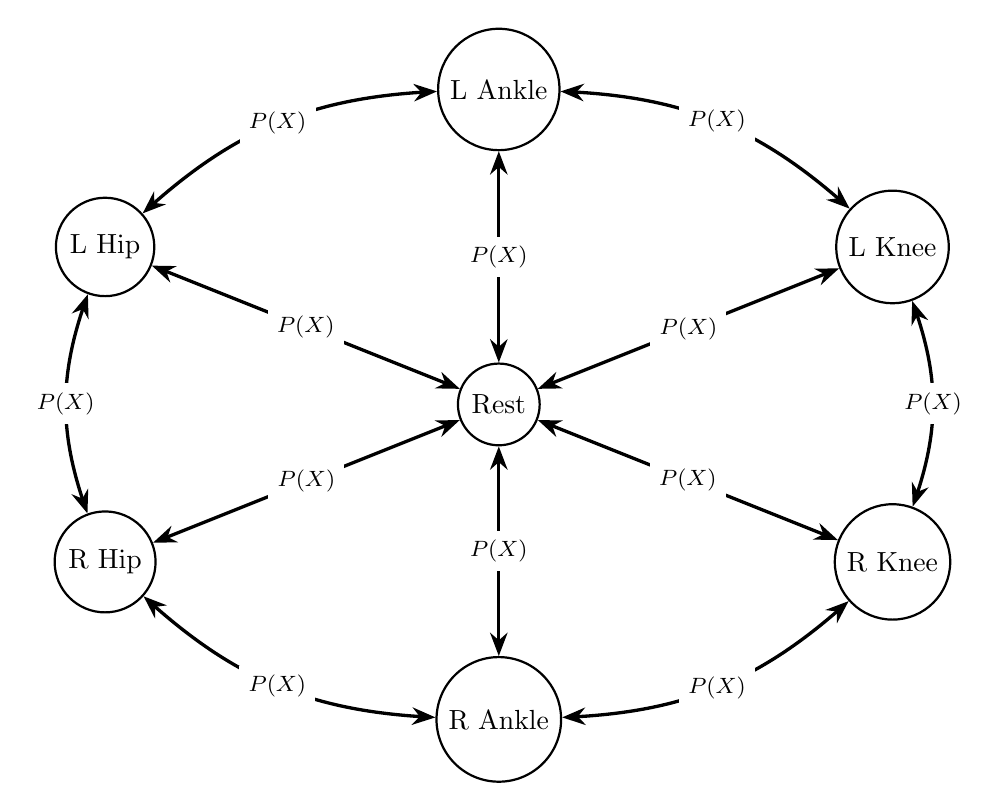
\begin{tikzpicture}
\begin{scope}[every node/.style={circle,thick,draw}]
    \node (Rest) at (0,0) {Rest};
    \node (LeftAnkle) at (0,4) {L Ankle};
    \node (LeftHip) at (-5,2) {L Hip};
    \node (LeftKnee) at (5,2) {L Knee};
    \node (RightAnkle) at (0,-4) {R Ankle};
    \node (RightHip) at (-5,-2) {R Hip};
    \node (RightKnee) at (5,-2) {R Knee};
    \end{scope}

\begin{scope}[>={Stealth[black]},
              every node/.style={fill=white,rectangle},
              every edge/.style={draw=black,very thick}]
    \path [<->] (Rest) edge node[pos=0.5] {\footnotesize{$P(X)$}} (LeftAnkle);
    \path [<->] (Rest) edge node[pos=0.5] {\footnotesize{$P(X)$}} (LeftKnee);
    \path [<->] (Rest) edge node[pos=0.5] {\footnotesize{$P(X)$}} (LeftHip);
    \path [<->] (Rest) edge node[pos=0.5] {\footnotesize{$P(X)$}} (RightHip);
    \path [<->] (Rest) edge node[pos=0.5] {\footnotesize{$P(X)$}} (RightKnee);
    \path [<->] (Rest) edge node[pos=0.5] {\footnotesize{$P(X)$}} (RightAnkle);
    \path [<->] (LeftHip) [bend left=20] edge node[pos=0.5] {\footnotesize{$P(X)$}} (LeftAnkle);
    \path [<->] (LeftHip) [bend right=20] edge node[pos=0.5] {\footnotesize{$P(X)$}} (RightHip);
    \path [<->] (RightHip) [bend right=20] edge node[pos=0.5] {\footnotesize{$P(X)$}} (RightAnkle);
    \path [<->] (RightAnkle) [bend right=20] edge node[pos=0.5] {\footnotesize{$P(X)$}} (RightKnee);
    \path [<->] (RightKnee) [bend right=20] edge node[pos=0.5] {\footnotesize{$P(X)$}} (LeftKnee);
    \path [<->] (LeftKnee) [bend right=20] edge node[pos=0.5] {\footnotesize{$P(X)$}} (LeftAnkle);
    \end{scope}

\end{tikzpicture}
\end{center}

Notably, they did not explicitly mention that one of the progressions could be from state to self state, but one can only assume this is true. So too, only seven states seems to limit the mobility of a patient.





\section{The Flagship in Synthesis}

\subsubsection{Founding Works.}

In large part, tremors induced by PD have already been well solved through deep brain stimulation and high intensity focused ultrasound. However, this paper focuses on some of the non-tremor symptoms of PD, and the idea that one can use spinal cord stimulation to fix degenerative diseases is generally interesting, so let us learn from\footnote{\url{https://www.science.org/doi/10.1126/science.1164901}}.The premise of this experiment is somewhat surprising, as stimulation is often thought to interrupt signals (as is the case in deep brain stimulation for PD, and SCS for neuropathy). In this case, though, they believe SCS \textbf{enhances locomotor signals}. That is, they are not treating PD tremors, but rather are treating PD induced akinesia. Experiments were performed in mice using dopamine-transporter knockout (DAT-KO) as their PD model. They also injected tyrosine hydrolase inhibitor (called AMPT)\footnote{I didn't bother Googling what this is, but intuition would suggest is aids in the conversion of tyrosine to catecholamines.} to further deplete dopamine. Dorsal root stimulation was performed using electrodes into the upper thoracic levels of the spinal cord. The greatest locomotor improvement in locomotion was found at 300 Hz stimulation.\newline

Notably, some hospitals are currently attempting clinical trials for spinal cord stimulation's use in treating Parkinson's. Some efforts include blocking pain and treating akinesia. \textcolor{blue}{Note from future Jackson: When I first read this paper a few months ago, I thought it was a bit silly. It was difficult for me to see why one would attempt this, when DBS is already so powerful. I figured it would go no where. Yet, read on:}

\subsection{SCS-DBS Intersection}

Here we discuss\footnote{\url{https://www.nature.com/articles/s41591-023-02584-1}}. Dr. Ashwin Ramayya, an MD-PhD neurosurgeon I had the pleasure of talking to, commented that after seeing this work his first thought was ``you don't have to be the best at everything." Indeed, this work is so awe inspiring that it makes one question their place in the field.\newline

DBS treats a very small subset of symptoms associated with PD. Because of the success of EES in treating SCI, these groups wondered if a similar feat can be accomplished in PD patients. The first bit of this work was done in an NHP model (rhesus macaque). Because of differences in monkey and human mobility, they developed a scoring technique to analyze PD models in NHPs and compare them to human PD symptoms. The preferred PD model for them was administration of MPTP (see section \textbf{\ref{sec:PDDegeneration}}!), a drug able to mimic the death of dopamine producing neurons. They compared spinal circuits before and after MPTP and identified ``hot spots" in the spinal cord. In implanting these devices, they stimulated different electrodes in the array in order to test their ability to cause muscle contraction. \newline

After these tests, they then aimed to use a brain-spine-muscle interface as they had in their other foundational works. Microelectrode arrays were inserted into the cortexes of RHPs and were able to regularly decode motor signals. They then furthered this by inserting EMG electrodes into the legs of NHPs\footnote{I am really wondering if some nice code can use this kind of data to iterate and self correct. Need feedback, of course.}. The neuroprosthesis together improved natural movement and posture. Finally, they added DBS to their circuit and found further improvement of movement. \newline

In humans, the ability to decode motor movement may be difficult in people with PD. Therefore, their first step was to recruit participants willing to get electrodes implanted into their cortex for reading their intended movements. They considered this a success and moved forward. They enrolled a patient in their STIMO-PARK clinical trial. The patient already had DBS, but still had some severe symptoms. They used a SCS paddle used in treating pain, connected to an Activa RC IPG, guided in location by CT and MRI. Rather than implanting an ECoG to read the patient's motor cortex, they instead used motion sensors and attempted to read motor intentions and send updated pulses to the stimulator that way. Fascinatingly, DBS and EES seemed to treat different symptoms at times, and act synergistically. That is, DBS${}^{ON}$-EES${}^{OFF}$ showed no improvement in ``fraction of time frozen," while DBS${}^{OFF}$-EES${}^{ON}$ showed total recovery. Their benefits were generally additive, though.\newline










\part[Some Ideas]{Some Ideas
            \vspace{0.2in}
            \begin{center}
            \begin{minipage}[l]{10cm}\small
                Man takes up the sword in order to shield the wound in his heart sustained in a far-off time beyond remembrance. Man wields the sword so that he may die smiling in some far-off time beyond perception. \newline
                -- Berserk by Kentaro Miura
            \end{minipage}
            \end{center}}

\chapter{Ramblings}

{\large \textcolor{red}{This section will largely be messy---likely for the coming years. It is for me to jot down ideas I have through reading.}}\newline

\section{Idealized World}

\subsubsection{Regarding ECoGs.}
Better ECoGs are really the path to incredible options. Of course, we have the mechanics already. Theoretically, one could simply build a mech-suit to accomplish any task---the trouble is getting it to respond. Somehow, it seems certain groups are able to resolve speech patterns and handwriting from brain data---so certainly it is within the realm of possibility. In this same way, ECoGs must become less invasive. The route to accomplishing this is likely through extremely intelligently made soft electronics. The resolution must be greatly improved by the inclusion of many, many more electrodes. In this way, powerful machine learning will be needed to process this data\footnote{I should really start teaching myself ML.}.\newline

There are a few things to consider. First, glial encapsulation will probably destroy you if you try to use too small of electrodes. Second, hard electronics seem to have many drawbacks. If you are using ultra-micro electronics, they are still limited by their ability to read within the gyri, given that the electronics will be hard. Similarly, you simply cannot afford to do massive cranioplasties on a regular basis. It'll need to be improved. Accompanying this issue is the ability to test on humans. One must first test on mice, which parallelly means that the device must be scalable. 


\subsubsection{Some Experiments.}


\begin{enumerate}
    \item Inhibit L-type VGCCs---likely need to use some kind of hydrogel with antagonists built in. 
    \item Optimize stiffness of paddles---or hydrogel, if we use the ACES system. 
    \item Optimize ECoG---that is, take up less space, maintain resolution, etc. to minimize invasiveness of surgery. 
\end{enumerate}

\subsubsection{Inhibit L-type VGCCs.}
It is well known by now that electrical stimulation combined with rehabilitation improves patient's ability to walk after SCI. 

\subsubsection{ACES Method.}

I like the ACES method as a starting point. It seems easy enough to implement, and can be built upon to arrive at some SCI method. Of course, I like that it is already integrated into a hydrogel setup. Some mild concerns are the 2 mA applied. It seems like quite a bit. 

\subsubsection{Biomaterials.}

The biomaterials possibilities are quite cool too. 

\subsubsection{CSF-cNs.}

A great, easy experiment is CSF-cNs ablation with EES, compare vs. WT, and see if recovery is similar.  


\subsubsection{Waveforms for Neuropathic Pain.}
Perhaps one can use a feedback mechanism, where the frequency of stimulation can be altered in order to dampen neural signals. You'd need to both read and write, essentially. Surely you can record brain waves responsible for feeling pain, and have a circuit edit itself to minimize them? $-->$ actually, dampening neural signals is a great example of a time to use the peak detection method, because you're only interested in magnitude. 

\section{Device Idea}

Another idea: frequency encoding of stimuli. Start by using EMG signal, digitizing it, using FSM to select a frequency output. In the distant future, this could be used to restore sensory perception after SCI or other injury. 






\subsection{Motivation}
Much is made of the frequency and amplitude of neuropathic pain stimulators. Dr. Ben-Haim even called the search for such as being the ``waveform revolution." Perhaps one can avoid this investigation altogether by simply connecting the entire pain pathway to the feedback loop of an opamp. That is, an opamps $v_+$ is grounded, the $\Vo$ is tied to a electrode in the spine, and the $v_-$ is connected to some form of ECoG in the brain. Theoretically, the opamp's $\Vo$ will do whatever it can to cause the signal read at the brain to go to 0. Of course, you cannot assume the opamp's feedback will be predictive, nor can you assume it will fix sharp pains. But, it may be able to fix chronic pain. Let's think of an overall build. 

\subsection{Framework}

\subsubsection{Processing Brain Waves.}
To process the brain waves we will likely:

\begin{enumerate}
    \item Filter out background from individual electrodes. 
    \item Subtract and amplify from some reference.
    \item Do some summing amplification from each of our electrodes.
    \item Rectify our signal.
    \item Convert via peak detection.
\end{enumerate}

\subsubsection{Feedback.}
To implement, we will then: 

\begin{enumerate}
    \item Feed processed signal to a PID controller of some sort.
\end{enumerate}

The only thing I am not sure about is if we will need a separate PID controller for each electrode in the spinal cord. I am not sure if we can just take all of the brain signals and combine them together, but I would assume that is fine. Another question is how much current we will need. If too low, we can add a push-pull to boost, but I doubt we will need a high current. 












%%%%%%%%%%%%%%%%%%%%%%%%%%

\vfill\pagebreak



\pagecolor{black}\afterpage{\nopagecolor}


       \vspace*{1in}
       
\begin{adjustbox}{minipage=10cm,scale={2}{3}}

       \textbf{\fontsize{30}{30}\selectfont \textcolor{white}{THANK YOU.}}\newline
\\

\end{adjustbox}

       \smallskip 

       \vspace{0.5in}

       {\fontfamily{phv}\selectfont \textbf{\Large \textcolor{white}{A FINAL NOTE: }}}

    \vspace{2cm}

        {\fontfamily{phv}\selectfont\textbf{\large \textcolor{white}{The world is always full of the sound of waves.\\ \\ The little fishes, abandoning themselves to the waves, dance and sing and play, but who knows the \textcolor{red}{heart} of the sea, a hundred feet down? Who knows its depth? \\ \\ -- Musashi by Eiji Yoshikawa}}}

    \vfill\pagebreak

\part{Addendum}

\label{sec:Addendum}

\section*{Overview}

Hello there! You've reached not only the end of the book, but actually the parts beyond its conclusion! At least for the moment, there are topics I'd like to discuss, but they're only tangentially related (if at all) to the idea of brain-machine interfaces. Therefore, consider this the bonus parts that are not worth reading, unless you are immensely inclined.\newline

One such topic is that of neurodegeneration. Naturally, there are not many direct parallels to be drawn from diseases like Alzheimer's and spinal cord injury. Yet, I do believe strongly in Musashi's epithet, that once you know the way broadly, you can see it in all things. For this reason, I think there is unknowable value is learning about degeneration. As it turns out, there are considerable parallels between the pathologies of traumatic SCI and neurodegenerative diseases, like degenerative cervical myelopathy (DCM) as covered in other sections like \textbf{\ref{sec:TvsnonTSCI}}. Thus, it is certainly worth understanding in-depth. Oh, and I because I am taking a class on it and I need somewhere to take notes ;) 




\chapter{Neurodegeneration}

This is more of a historical dive into the research, because so much of what we know about neurodegenerative diseases is likely wrong, overstated, or misinterpreted. There are many fascinating theories and little agreement. You will hear some, like Dr. Rothstein at JHU, argue that there is a viral component. You will hear some, like the Wallace lab at Penn, claim that Alzheimer's is due to mitochondrial dysfunction and not amyloid aggregation. So for now, let's call this a historical review of the research up to this point.\newline

\textcolor{red}{This is all extremely messy and disgusting for the moment. Will clean up later (hopefully).}\newline

\section{Alzheimer's}

\subsection*{Overview}

Alzheimer's disease (AD) is a neurodegenerative disorder found in many elderly patients, and the disease confers memory loss and other forms of cognitive decline. It can be familial or sporadic, and while onset typically begins much later in life, some early onset forms exist. Sporadic Alzheimer's is so ubiquitous that some hypothesize that it borders on the normal aging process. It is this ubiquity that makes it the \textit{holy grail} and or the \textit{white whale} of disease---solving it would help endless people. In the United States, it affects around 6 million people, making it more common than all cancers combined\footnote{\url{https://www.alz.org/alzheimers-dementia/facts-figures}}$^,$\footnote{\url{https://www.cancer.org/research/cancer-facts-statistics/all-cancer-facts-figures/cancer-facts-figures-2022.html}}. It was first characterized by Alois Alzheimer in 1906, who used dyes to stain tissues and reveal their histology. He found strange plaques present outside of neurons, and stringy tangles within them. Alzheimer's disease must be diagnosed after death because of considerable overlap with other disease symptoms---that is, nailing down memory loss to specifically AD is impossible without analyzing brain histology. Such a diagnosis is done on the basis of extracellular amyloid plaques and intracellular tau tangles, discussed later.\newline

While, generally speaking, we are helpless in tracking and managing AD progression in patients, some tools exist. For example, a drug called aricept blocks acetylcholine degradation, which can slow symptoms for a short time. Measuring amyloid buildup, or other markers, in the CSF is a tool to determine disease progression and or drug efficacy. Congo red is used to stain any amyloid buildup---that is, it stains any $\beta$-pleated sheet and is not specific to the $\beta$-amyloid of AD, but still can be of help. Another method is using thioflavin T (ThT), which also interacts with $\beta$-pleated sheets. This has been used to make a radioactive compound called Pittsburgh compound B (PiB), which can be imaged on a PET scanner, and used to quantify the amount of plaques in a living patient. PiB is presently the best available compound and helps identify AD years before dementia begins.\newline

All of our modern understanding of AD comes in just the last few decades. For the purpose of these Neurodegeneration sections, put yourself in the mind of someone in mid-late 1980s: genetic testing was a blooming but still a young field. Sequencing genes was immensely difficult, but worse was finding the correct region to sequence. Linkage studies helped give indications of location, but one still was leagues away from nailing down a couple kB region to sequence. It was completely unknown what genes, if any, cause AD. In fact, only a couple genes and proteins were known at all. We were totally blind to the human genome. But, we did have something: the protein.\newline

$\beta$-amyloid was purified in 1984 by Glenner and Wong\footnote{\url{https://www.sciencedirect.com/science/article/pii/S0006291X84801904?via\%3Dihub}}, which allowed it to be sequenced early. The protein was small, but congregated together into plaques. They generated an antibody against it, allowing them to stain and identify regions of the brain affected by AD. After the $\beta$-amyloid protein was identified, other groups sequenced the surrounding nucleotides and found it to be part of a larger transmembrane protein---which was eventually called the amyloid precursor protein (APP). Thus, it was intuited that this little peptide was cleaved from the larger transmembrane protein. Fascinatingly, trisomy 21 patients almost ubiquitously get AD, and specifically early onset AD---suggesting there must be some association with Chr21, and perhaps some correlation to dosage. Other genetic linkage studies confirmed this, showing that in familial AD, there was some segregation with Chr21. So, we had the protein, and we have a general idea of location. Where do we go from here?

\subsection*{Finding APP}

% \subsection*{Goate et al, 1991} 

As mentioned, the A$\be$ protein was first sequenced in 1984. In 1987, four groups cloned the APP gene. However, it remained completely unknown if this protein was causative. It was in 1991 when Goate et al. confirmed the existence of causative mutations in the APP gene\footnote{\url{https://www.nature.com/articles/349704a0}}.\newline

To begin investigation, groups had to focus on familial AD (fAD), otherwise finding a non-inherited mutation would be nearly impossible. In these days, only a small set of chromosomal markers were known. However, these markers allowed for the powerful scanning of different regions of the chromosome. That is, you could compare markers between different family members, indicating different degrees of recombination. Family members sharing the disease and similar chromosomal markers allowed you to narrow down to a region of interest, implying the causative mutation was somewhere nearby. This was quantified by logarithm of the odds (LOD) scores, where more positive numbers meant the association was more likely. Generally, LOD scores above 3 give a high level of confidence that the disease segregates with said marker. This required finding large enough pedigrees where this kind of analysis was possible. Of course, misdiagnoses would immediately ruin these sorts of analyses. Similarly, heterogeneity in a disease would greatly complicate things. Indeed, this is why APP, for a long time, was not thought to be the causative gene in AD---many families showed no segregation with APP at all. \newline

In their first early onset AD pedigree, Goate and colleagues found family members to exhibit two different alleles, which correlated exactly with AD. However, two unaffected family members exhibit recombinant alleles at different sites. The first individual shares the same allele at the telomeric end of the chromosome to their affected parent. This individual was 15 years over the mean age of diagnosis for AD, giving a high degree of confidence that they do not have the disease. This suggests the AD causing gene is not, in this family, telomeric to the APP gene. The second individual shared the same allele as the affected parent only centromeric to APP, and at the time of the study was unaffected. It's possible this individual would develop AD later in life. Therefore, based on their current pedigree, APP was the clearest possible disease causing gene, but they did not have absolute confidence.\newline

From there, they used PCR to identify the site of mutation and developed primers specifically around the $\beta$APP. This was a natural choice, as A$\beta$ was already identified in AD plaques and, fascinatingly, dysfunction of the $\beta$ unit was implicated in other diseases already. Via direct hand Sanger sequencing, they found a valine to isoleucine polymorphism in the $\beta$APP encoding portion. \newline

\subsubsection*{Digression: Restriction fragment length polymorphism (RFLPs)}

Harnessing the power of restriction fragment length polymorphism (RFLPs) immeasurably advanced genetic testing. The benefits of RFLPs are that mutations cause a restriction enyzme cut site---allowing for very easy screening. Researchers would look for polymorphisms around a disease causing gene, which served as an easy technique for getting a broad sense of the genotypes in a pedigree. In other words, it helps you screen for markers segregating with the disease causing gene. Better yet, when a polymorphism that's thought to be disease causing is found, one can see if it alters a possible restriction enzyme cut site. For example, perhaps the polymorphism converts an \textit{EcoR}I cut site into a non-cut site. Now, to screen possible patients, instead of sequencing every patient individually, they could use PCR and restriction enzymes and analyze the bands on a Southern blot (two would signify no mutation, one would signify mutation), significantly cutting down the time, effort, and cost of diagnosis. While sequencing may take closer to weeks, such enzyme gels can be done in an afternoon.

Indeed, a \textit{Bcl}I restriction site induced by the polymorphism, allowing them to detect the presence of the mutation on a gel. In this case, a non-affected person will have an uncut sequence of DNA of 319 bp in length, while those affected individuals will have a band at 199 bp and 120 bp. They were able to screen other families and find the same mutation. To verify these families were not related, they checked other polymorphic sites and found divergence, suggesting sufficient genetic dissimilarity.\newline

Therefore, these authors identified a site on Chr21 that segregated, sometimes, with early onset Alzheimer's disease and in the gene encoding amyloid precursor protein (APP), specifically within $\beta$-amyloid. Importantly, this mutation was conserved between two fAD pedigrees, implying it was indeed causative. Because segregation of this gene is not found in all AD patients, the authors concluded there must be considerable heterogeneity among early AD patients. They also hypothesized that APP's lack of causative support may be due to previous studies using patients with misdiagnosed AD with other diseases that phenocopy it. Notably, they did not sequence the entire APP gene. Thus, it's possible that the true disease-causing mutation is not within the $\beta$ encoding portion. Their Discussion included the suggestion that the mutation, being valine to isoleucine (becoming more nonpolar), makes the APP transmembrane domain anchored more tightly to the membrane---which we now know is false, but it's still interesting to see where their heads were at in these all-important early days. They did correctly postulate that the deposition of $\beta$-amyloid is associated with a worsened disease, and based on the phenotype of trisomy 21, it is somehow dose-dependent.

\subsubsection*{Follow-Up Work.}

Brain banks have been an instrumental, and highly controlled way to investigate neurodegenerative diseases. Access to a brain bank could make or break researchers. After this work, many of the labs around the world began sequencing A$\beta$ from their brain banks, and a host of mutations was found. There seemed to be a correlation between the location of mutations and the site that a protease cleaves APP. A number of secretases cleave APP, in different orders. We now know that when $\alpha$-secretase precedes $\gamma$-secretase cleavage, two fragments of A$\beta$ are formed---this is not pathogenic. However, when $\beta$-secretase precedes $\gamma$-secretase, leading to slightly different fragmentation, problems arise. $\gamma$-secretase cleavage is also not hyper-specific to a given site on APP, and thus some variable cleavages too lead to worsened disease. $\gamma$-secretase cleaves many other proteins in addition to just APP as well.


\subsection*{Finding the other AD Loci}

Other linkage studies had identified more chromosomal locations associated with AD. To this point, there were three loci known: $\beta$APP, ApoE (discussed later), and an unnanmed one called AD3. This AD3 loci was associated with an aggressive form of AD, making it ripe for identification. It was Sherrington et al. in 1995 who finally found it\footnote{\url{https://pubmed.ncbi.nlm.nih.gov/7596406/}}.\newline

The loci was loosely mapped to Chr14. Using a group of familial pedigrees and previously published data, they examined a set of genetic markers on Chr14. By analyzing the recombination events, they were able to conclusively narrow the causative region to between two markers. However, this region was still massive and likely contained many hundreds of genes. To clone the region, they started by generating contigs. They examined the partial haplotypes of families with the same ethnic origin, hoping to further narrow down a region of interest. Two clusters of genes were shared between families of the same ethnicity. This indicated to them the heritability of the gene, and allowed them to make more direct comparisons as the families were under similar ``genetic backgrounds" (that is, comparing between very heterogenous groups can make it difficult to discern causative mutations and genetic noise). They analyzed the cDNA clones of this region and determined 151 of them to reflect spliced mRNA. Using RT-PCR from AD affected brains and non-affected brains allowed them to narrow their field of interest to 7 transcripts. Among these was a novel gene, represented by fragment S182---encoding for a newly identified, transmembrane protein. They identified mutations in this new protein that were conserved between families, indicating these defects are causative.\newline 


Using a Northern blot, they identified 2 major transcripts and expression in most regions of the AD brain. Notably, mouse tissue only identified one of the two, specifically the 3kb region---which the authors suspect may be the normal mRNA, and the other the other transcript may represent a more rare, alternatively spliced version. \newline

There is considerable sequence homology between the mouse and human transcripts. They used computational algorithms to predict 7 transmembrane domains and an accompanying possible structure. Two other non-polar regions were found that appear unstructured and unlikely to form transmembrane helices. They identified potential glycosylation sites, which they suspect may help order these regions into structures along the membrane. It was not presented in their data, but Sherrington and colleagues commented on sequence homology with \textit{C. elegans} proteins---it was hoped that similarity to proteins mapped in lower order organisms may give insight into what this protein was. Unfortunately, no great candidates stood out among those identified. A protein called SPE-4 seemed to be the most similar, which plays a role in spermatogenesis specifically through a golgi derived organelle formation---thus the authors throw out the possibility of S182 altering $\be$APP or Tau golgi trafficking. Of course, we know in hindsight that this is untrue. A similarly offered hypothesis is that this S182 is the mammalian equivalent of Ca-$\alpha$1D\footnote{This is funny to no one but myself, as my first published paper was on Ca-$\alpha$1D function in \textit{Drosophila}, a cool 28 years after this paper came out.}! \newline

Within the ORF of this S182 gene was mutations in multiple AD affected individuals. Among families with such mutations, no unaffected family members were ever found to have these mutations. In short, this strange, S182 gene encodes for a transmembrane protein whose function is presently unknown. This gene would eventually be called PSEN1. 

\subsection*{PSEN and the Amyloid Cascade Hypothesis}

% \subsection*{Strul \& Greenwald, 1999}

\subsubsection*{Background.}

Soon after PSEN1 was identified, another gene was found on Chr1, which happened to be quite similar to PSEN1. We now know this to be PSEN2. Then, a \textit{C. elegans} paper came out in which a worm homolog was found, identified through investigation of Notch signaling. In hindsight, we know that $\ga$-secretase and PSEN are one and the same (or rather, that PSEN1 is the proteolytic subunit of the $\ga$-secretase complex).\newline

Now, for the formal introduction: Prenesilin (PSEN) is a transmembrane protein known to contribute to AD progression, and thought to play a role in amyloid processing. In \textit{Drosophila}, PSEN modulates Notch activity, which thereby can influence transcription. Notch signaling is a key developmental path in many organisms. Notch is especially important in cell-to-cell communication during development, aiding in cross talk between cells and driving cell differentiation. A ligand released by a cell will bind to Notch's extracellular domain, inducing a conformational change and allowing its intracellular domain to be cleaved. Cleavage is done by $\ga$-secretase, which cleaves the Notch intracellular domain (NICD). The NICD is trafficked to the nucleus, where it interacts with gene inhibitors, turns them off, and allowed genes to be transcribed.\newline

Model organisms, like \textit{Drosophila}, were instrumental to our understanding of PSEN, and much of this understanding came from Strul \& Greenwald, and Ye et al., published in the same issue of \textit{Nature} in 1999\footnote{\url{https://pubmed.ncbi.nlm.nih.gov/10206646/}}$^,$\footnote{\url{https://pubmed.ncbi.nlm.nih.gov/10206647/}}. They found that PSEN is needed for Notch cleavage, allowing it to exit the membrane and enter the nucleus where it can exert its control.

\subsubsection*{The Key Works.}

Let us begin with Strul \& Greenwald. By 1991 work, it was known that $\beta$-secretase is required for APP's conversion to $\beta$-amyloid and such cleavage occurs in the extracellular space. Similarly, it was known that $\ga$-secretase cleaves APP in the transmembrane domain. It was shown that Notch cleavage occurs in a similar way. PSEN mutations cause AD by increasing the amount of A$\be$. PSEN knockdown inhibits the activity of $\ga$-secretase. It was not known at this point if PSEN was an activator or a component of $\ga$-secretase. Notably, they specifically comment on PSEN in relation to an A$\be$42 (42 amino acids in length) variant, which is mentioned in other literature. Some thought that variable cleavage in the APP gene leads to slightly different length A$\beta$ products, which are more or less prone to aggregation.\newline

The pair began by analyzing the phenotypes of PSEN (PS in flies) knockdown. They generated two truncated alleles, which both showed identical phenotypes. \textit{PS}$^-$ embryos exhibited clustered neuroblasts, which should typically be spread out. Midline cells, thought to be controlled by Notch, did not differentiate as they do in WT flies. Homozygous \textit{PS} loss was pupal lethal. Clones of \textit{PS}$^-$ cells causes abnormal wing development, thought to be through Notch's role in dorsal-ventral cell communication. Though, embryos of \textit{PS}$^-$ flies show normal accumulation and membrane localization of Notch, which indicates that it is not upstream of Notch expression---suggesting a role in Notch signaling.\newline

They then generated a Gal4 knock-in on the intracellular side of the Notch protein. This tool was used to determine Notch localization. This was marked by a UAS (a promoter), which drives $\beta$-Gal expression (in the presence of the Gal4 protein) that they can stain for. I.e., when Notch is trafficked to the nucleus, $\beta$-Gal is expressed and can be stained for. They then used three 3 lines, which they call: N$^+$-GV3, N$^{ECN}$-GV3, and N$^{intra}$-GV3. N$^+$-GV3 is like their WT control, which functions normally. In the absence of either PSEN (PS$^-$) or Notch's ligand (Delta, Dl$^-$), no nuclear transport occurs, marked by no $\beta$-Gal staining. N$^{ECN}$-GV3 includes a large deletion of the extracellular domain, which essentially decouples Notch from it's ligand and makes it constitutely active. Thus, in this case they found Dl$^-$ embryos to still have considerable trafficking to the nucleus, while PS$^-$ did not. Finally, N$^{intra}$-GV3 is missing both the extracellular and transmembrane domains---therefore suggesting it will never be trafficked to the membrane at all, causing it to remain cytosolic. In this case, neither Dl$^-$ nor PS$^-$ prevented Notch trafficking to the nucleus, so all embryos could be stained by the $\be$-Gal.\newline

Onto Ye et al: to investigate the role of PSEN in Notch signaling, they developed 5 deficiency (\textit{Df}) lines and observed similar dysfunction mentioned in the previous paper. \textit{Df} lines are large chromosomal deletions, spanning many genes. Therefore, to verify the phenotypes of these lines were PSEN dependent, they used a variety of DNA rescues in order to see WT phenotypes. One of their rescues omitted PSEN DNA and did not rescue the phenotype of these flies. Therefore, they felt confident that these \textit{Df} lines served as good models of PSEN mutation and or knockdown.\newline

When analyzing their \textit{Df} lines, they identified a pupal lethal phenotype they considered to be similar to an Su(H) mutant, an effector of the Notch signaling path. They used a variety of wing disc markers ($\be$-Gal driven by expression of genes related to wing development), and saw $\be$-Gal missing or heavily altered in their \textit{Df} lines. Similarly, sensory organ precursor (SOP) cells were found to cluster together with limited lateral inhibition, determined by enlarged territories and increased \textit{achaete} and \textit{scabrous} expression (early SOP markers).\newline

The \textit{Df} lines showed obvious neurodvelopmental issues, including unclear and or non-existant formation of a ventral nerve cord (VNC), scattered neural localization, and over-proliferation. This experiment was done via ELAV staining, a pan-neuronal marker. Interestingly, they saw that paternal PSN partially rescues neurodevelopmental troubles---VNC formation was visible, but clearly had uncouth morphology.\newline

Notch protein localization and expression was similar across their PSEN mutants and wildtype larva. This was consistent between both the intracellular and extracellular components of Notch, and for the Notch ligand, Delta. In retrospect, the finding that intracellular PSEN is unchanged may be considered surprising, since PSEN is now known to cleave Notch. The authors attribute this to the small intracellular quantity that is actually trafficked to the nucleus, which therefore may remain undetectable using immunostaining. To investigate how PSEN processes notch, the authors used Western blots. The largest, $\approx$120K band of the Notch protein migrates more slowly in the PSEN mutants, suggesting the piece is slightly larger. Among the 120K fragments, the largest dominates in the PSEN knockout compared to WT. This phenotype is specific to PSEN knockdown, as in the Su(H) mutant background, this phenotype is not observed (i.e., Notch is processed as WT is), and similarly in mutant Notch background the large 120K band is absent. The same fragments are unaltered in other proteolytic knockdown (specific to Notch's processing in the golgi), demonstrating a specificity for PSEN and that the cleavage observed occurs after its membrane targeting.\newline

Expression of Notch's intracellular domain alone, and accompanying blots, showed that it is unaffected by the PSEN knockdown, suggesting PSEN plays a role specifically in releasing Notch from the membrane. Finally, PSEN knockdown did not affect Delta levels, as quantified by Western blots. Inactive Notch confers proneural clustering in both WT and PSEN mutants. Using only the intracellular Notch domain, no SOP differentiation occurs in both WT and PSEN mutants. Most SOP differentiation was suppressed in a membrane tethered background. It is supposed by the authors that PSEN is not required for membrane trafficking nor nuclear trafficking of Notch. Rather, they supposed PSEN is needed in some activation mechanism that follows ligand binding.\newline

The experiments by both groups led to the conclusion that PSEN was specifically involved in cleavage of Notch, as opposed to acting as a ligand or aiding in it's downstream signaling cascade. It was concluded that PSEN cleaves Notch somewhere in its transmembrane domain. Naturally, the big takeaway was that PSEN may play a similar role in APP processing, and thus produces A$\be$ in the same way.


\subsection*{Making an AD Mouse Model}

First, let me state that mice do not naturally get Alzheimer's disease. This is a key point that I think often remains understated. Flies, similarly, do not get AD. In fact, it is difficult to get protein aggregation in both of these models. Many fly ALS models (discussed later) do not show aggregation at all, while the same proteins in humans do. Therefore, one must always wonder if the models use are using non-physiological conditions to achieve them (e.g., absurdly high doses of some protein, which may, on their own, have odd implications). \newline

To this point, we have a decent idea of some of ``key players." But, we have little room to investigate them. Despite some attempts, no successful AD model had been established 1995. Goate et al. were the first to generate a meaningful one\footnote{\url{https://www.nature.com/articles/373523a0}}. The group used a modified, transgenic APP gene in mice which reproduced many of the AD phenotypes. Such a model drove increased expression in many mouse tissues, but especially within the brain. They consider the promoter they used, PDGF-$\be$, and the familial AD mutation they used (V717F), to be the two prime contributors to success.\newline

Their Northern blots showed 3 different alternatively spliced forms of APP mRNA, and Western blots showed the amount of protein is was increased in the transgenic mice vs. WT mice, and that that A$\be$ was indeed being produced too. Recall that these mice did have endogenous APP of their own, which was not mutated. Therefore, the disease focused on the gain of function associated with APP aggregation.\newline

A$\be$ buildup occurred only at 6-9 months of age and worsened from there. It was primarily local to the hippocampus, corpus callosum, and cerebral cortex. A$\be$ buildup took a variety of forms, including irregularly shaped bundles and other more characteristic, dense plaques. Reactive astrocytes were often found surrounding such plaques via GFAP staining. A$\be$ plaques were associated with synaptophysin, suggesting their localization to sprouting axons\footnote{It is a bit unclear what is meant by sprouting here---I am not sure how definitions of sprouting may differ between groups.}. Staining for MAP-2 in addition to synaptophysin showed plaques disrupting and de-densifying nearby regions. Plaques also seemed to compress the surrounding neurophil (the unmyelinated, cell dense regions of neural tissue). 

\subsubsection*{Tangled up in Blue.}

The appropriate question to ask is: ``what about tau?" Tau was not found in this model. Tau is notoriously absent from rodent tissues. At the point this model was created, there was the belief that the ratio of A$\be$42 to 40 indicates the progression of the disease, which existed under the umbrella of the amyloid cascade hypothesis. The vast majority of the work done so far focused on the plaques, but with no insight whatsoever into the tangles.\newline

 In the 60s, tangles were purified to the point of visual analysis, indicating they were helical in nature and likely two filaments coiled around one another. This gave them the name ``paired helical filaments" (PHF). In 1992, this PHF was tested against tau antibodies and stained with Coomassie Brilliant Blue\footnote{The section name is a play on the Bob Dylan song title.}, showing different forms of tau at variable molecular weights. Normal, wildtype tau was largely unaffected by dephosphorylation by a generic phosphatase. But dephosphorylating PHF substantially lowered the observed molecular weight. In short, this suggested PHF is a heavily phosphorylated version of tau. This principle is generally conserved in diseases, where a protein becomes abnormally phosphorylated and aggregates. Notably, tau mutations are never associated with familial AD---but are associated with other degenerative diseases.\newline

 The endogenous function is not fully solved, but we know the gist. Tau binds to microubules and is thought to help stabilize them. When phosphorylated, it unbinds from the microtubules, thought to cause axonal degeneration. Notably, tangle burden progresses with the disease more so than does plaque burden. Tangles appear later on, but correlated more strongly with increased symptoms. This bit of conflict created a rift among scientists on what the root of the disease was---A$\be$ or tau. Some supposed tau was a side effect of the greater disease, induced by A$\be$ aggregation. Others supposed that A$\be$ aggregation was largely benin, and it was when tangles arose that the disease truly began. 

 \subsection*{What About Tau?}

 Initially it was thought that tau tangles were solely a symptom, and or, a result of already dying neurons. In 2000, Lewis et al. helped challenge this idea with a paper that overexpressed mutant tau protein found in frontotemporal dementia and parkinsonism (FTDP)\footnote{\url{https://www.nature.com/articles/ng0800_402}}. The mice exhibited a wide variety of degeneration linked to the tau protein buildup. This included symptoms even in the spinal cord and peripheral nerves. Mutant tau (P301L) was expressed by the mouse prion promoter (MoPrP). They found that hemizygous lines expressed tau at approximately the same level as WT, and mice homozygous for the mutant expressed it at levels $\approx 2\times$WT.\newline

 A composite of behavioral assays, including escape responses, motor defects, and the inability to right (flipping over from its back onto its feet again) demonstrated sensorimotor dysfunction. Hemizygous mice had symptom onset at about 6.5 months, while homozygous at around 4.5 months. Eventually, they were unable to walk. \newline

The spinal cord showed defects, namely fibrillary gliosis, axonal degeneration, and axonal spheroids (bleb). GFAP immunoreaction was found throughout the brain, signifying gliosis. Importantly, degeneration was global, including skeletal muscle and peripheral nerves. Neurofibrillary tangles were found throughout the brain, including in the brainstem and diencephalon. Interestingly, so-called ``pretangles" were found in other regions of the brain, including the hippocampus. The fibrils were irregular in shape and specifically phosphorylated.\newline

In the mutant lines, a greater proportion of tau was insoluble and shifted toward a higher molecular weight. This is consistent with being heavily phosphorylated, which was verified by dephosphorylating the protein causing the elimination of such high-weight bands. The authors showed the similarity between AD bands and their model's bands. 

\subsubsection*{Implications.}

To follow-up, whether or not APP modulates the tau protein buildup became a focus. Indeed, crossing this tau mouse with an APP mouse led to increased NFT formation. Later, groups tried combining multiple familial AD mutations in APP with PSEN mutants, leading to very early onset and more powerful, clear behavioral defects. After these tau models were verified, tau too was added. It isn't clear what the connection between fAD and sporadic AD is. Is inducing these severe AD symptoms in mice via fAD mutations actually comparable to the very slow progressing, late onset forms of AD? To what degree are the fAD and sporadic AD mechanisms conserved?\newline

In clinical trials, antibodies against A$\be$ showed the ability to decrease plaques. However, no obvious clinical benefit was found. Naturally, this could be because degeneration had already run its course, or it could be that tau is directing progression at this point. Some take this as evidence against the amyloid cascade hypothesis. 


\subsection*{Mutations Protecting Against AD}

 In 2012, Jonsson et al. found something totally unexpected\footnote{\url{https://pubmed.ncbi.nlm.nih.gov/22801501/}}. By 2012, gone were the days of hand reading base pairs from an autoradiogram. The intense study of amyloid precursor protein's (APP's) role in Alzheimer's disease (AD) largely began when Goate \textit{et al}. hand sequenced the $\beta$-amyloid coding region of individuals with familial AD and found a causative mutation. Some 20 years later, the $\beta$-amyloid allele of nearly every individual in Iceland became known. Iceland keeps quite good genealogy records, and because people are quite related due to population isolation, their genetics are ripe for this sort of testing.\newline

Via direct sequencing of around 2,000 Icelanders, Jonsson et al. generated chips for APP alleles, allowing for the genotyping of 70,000 more. The accuracy of their genotyping was verified through direct sequencing, allowing computational approaches to provide predictions for nearly all Icelander's APP allele. Fortunately, an otherwise very rare allele is present at a high frequency in some North European countries, like Iceland. This allele was A673T, the first mutation found to be protective against AD, and its discovery indirectly answered a number of open questions. \newline

The group demonstrated this A673T mutation is protective through comparisons of the allele frequency in AD and non-AD patients. Notably, this allele was 7.52 times more likely to be found in cognitively intact individuals above 85 than in AD patients, suggesting it aids in the prevention of late onset AD. Like many familial AD mutations, A673T is present near the $\beta$-secretase 1 (BACE1) cleavage site. Because the A673T mutation is protective against late onset AD, it indeed showed APP's sequence is relevant to sporadic AD, and that there is some conserved mechanism between early onset and late onset AD. Through Western blot analysis of 293T cells (kidney cells), they sought to gain mechanistic insight. Interestingly, the work showed evidence against the importance of A$\beta$ cleavage product ratios (namely A$\beta_{42}$ to A$\beta_{40}$). The A673T mutation showed an overall decrease in A$\beta$, rather than affecting this A$\beta_{42}$ to A$\beta_{40}$ ratio. The amount of sAPP$\alpha$ was slightly raised, as might be expected if un-cleaved APP is present in higher levels due to weakened BACE1 activity, making more available for cleavage by $\alpha$-secretase. These results suggest AD  can be slowed or stopped via reduction of A$\beta$, particularly through the weakening of BACE1 proteolytic activity. They make the bold claim that the A673T mutation is protective against general cognitive decline, suggesting a function of APP beyond AD. This measure was done by the Cognitive Performance Scale (CPS), but is purely correlative in nature.\newline

The mutations compared by Jonsson  and colleagues were A673T and A673V, with A673V showing a significant rise in A$\beta$. Notably, A673V converts from the mildly hydrophobic residue, alanine, to the markedly more hydrophobic residue valine. Conversely, A673T becomes more hydrophilic. One can postulate that the cleavage of APP, releasing A$\beta$, requires a hydrophobic interface between BACE1 and APP around this residue. Further credence is given to this by a different familial AD mutation, called the Swedish mutation (K670N/M671L), which adjacent to the BACE1 cut site becomes more hydrophobic with leucine.\newline

Mudher and Lovestone stated that proving the amyloid cascade hypothesis requires showing a reduction in plaques results in tau tangle abolishment, and thus functional recovery\footnote{\url{https://pubmed.ncbi.nlm.nih.gov/11801334/}}. A considerable drawback of Jonsson and colleagues' work is that there is no direct insight into the interplay of APP and tau. The study of AD still has long to go before reaching its completion. But, as new tools become available to researchers, progress is continually made. Faster sequencing, computational drug design, and ever-improving mouse models allow for new routes of study. The journey to treating AD is long, but we can be sure that whenever a new roadblock arises, technological advancement will provide the path to new insight. 

\subsubsection*{Digression: Other Means of Protection.}

Interestingly, education proves to be a strong protective factor against AD. If memory problems have already began, using acetylcholine-esterase inhibitors can be helpful to help potentiate this transmitter and improve function (or, delay its decline). However, these forms of treatment tend to be short-lived. Exercise also turns out to be quite helpful in promoting neurogenesis, which may delay progression.


\subsection*{There's Still More?: ApoE}

As mentioned in an earlier section, the effect of ApoE on AD had long been known. Surprisingly, ApoE protein was found within the A$\beta$ plaques, and only after this was a linkage found to Chr19, around the APOE gene. ApoE is a small protein, only 229 amino acids. It is a lipoprotein, which helps move cholesterol through the bloodstream---therefore, one possible mode of management is controlling cholesterol levels. Four alleles exist, but the three key APOE alleles we consider here are: 

\begin{enumerate}
    \itemsep 0em
    \item APOE-$\epsilon$2 (cys112, cys158)
    \item APOE-$\epsilon$3 (cys112, arg158)
    \item APOE-$\epsilon$4 (arg112, arg158)
\end{enumerate}

The dosage of the APOE allele which confers risk of disease, as shown by Corder et al. in 1993\footnote{\url{https://pubmed.ncbi.nlm.nih.gov/8346443/}}. The APOE-$\epsilon$3 allele is the most common. It is thought, now, that ApoE2 may be slightly protective over ApoE3. But, the key player is  APOE-$\epsilon$, whose presence results in a much earlier age of onset. The APOE-$\epsilon$4 allele is one of the strongest determinants of AD onset. The risk factor for AD increased by approximately $3\times$ for each additional APOE-$\epsilon$4 allele. Corder and colleagues showed that $\approx 90\%$ of those with 4/4 genotype had the disease, while only 19\% did for a 2/3 genotype. Similarly, the age of onset was much earlier for those with 4/4 than other genotypes. Autopsies of these patients show a much higher degree of amyloid staining, suggesting the APOE-$\epsilon$4 allele increases the plaque burden.\newline 

From then to now, there has been considerable skepticism over this finding. As APOE is not considered disease causing, but rather a risk factor, it was unclear the role it might play. Still, some were unconcerned with the fact that ApoE shows up in plaques, as it is not clear that amyloid is disease causing. Importantly, too, most of these genetic studies were done in European populations---which turned out to be of great relevance. APOE-$\epsilon$4 is not a (big) risk factor in Hispanic populations like it is in a European background, further muddling the potential role that it may play. 


\subsection*{Degeneration \& Genome Wide Association Studies (GWAS)}

Sporadic AD remains much more common than familial---so how do you go after risk factors involved in sporadic AD? Of course, APOE-$\epsilon$4 is the highest risk factor by a significant amount, but are there more\footnote{It is unclear to me if asking this question is a good idea. Perhaps we should focus on understanding the factors we already have identified first. Or perhaps we will find the missing link that connects all the puzzle pieces.}?\newline

One way to investigate this is through a genome wide association study (GWAS). A Manhattan plot is one way to represent this data, and probes the entire genome for SNPs of individuals and co-segregates significantly with diseases vs. controls. Initially, massive amounts of money were poured into GWASs, but were largely unsuccessful. Now, with much greater sample sizes, they have been more successful. Notably, 90\% of polymorphisms are shared ancestrally. Around 60 de novo point mutations are expected per individuals, with 3 indels, and (on average) less than 1 structural variation. Therefore, much of the original GWAS studies were muddled by the different genetic backgrounds of the patients. That is, someone with the disease from one continent that is compared with an individual of another continent would show a significant, surprising degree of genetic association for factors totally unrelated to the disease. Combining this with the fact that a large portion of the genome is non-coding---GWAS struggled greatly with poor controls in the early days.\newline

Now, suppose you find a peak---what next? You have to understand what is occurring. If the mutation is in an enhancer, what gene is it affecting? When tons of genes cluster closely together, and linkage is found, which one is the affected gene? When many nearby SNPs are found, which ones are relevant? In short, GWAS seem like an all-powerful technique, but often the results are difficult to interpret or meaningless. Later, in section \textbf{\ref{sec:HDGWAS}}, we will discuss a hugely successful example of this mode of study. 


\subsubsection*{Digression: AD and Sleep.} 

This is from a video featuring Holtzman called Sleep \& the Pahophysiology of Alzheimer's Disease\footnote{\url{https://www.youtube.com/watch?v=zCmngDk9VDU}}. To start, dementia is considered a decline in cognitive abilities sufficient to impair daily life. Approximately 50\% of people over the age of 80 have some form of dementia.\newline

The role of glia has been understated for a long time in the progression of AD. It seems that Tau and $\beta$-amyloid buildup activates a glial / autoimmune response. Like most neurodegenerative diseases, symptom onset marks the end stages of it. Pathology beginnings occur far before symptom onset.\newline

APP is enriched at synapses in the brain. Interestingly, endocytosis occurring at the membrane leads to membrane bound APP being taken back up by vesicles into the synapse. It is here that, while in endosomes, APP is cleaved, leaving behind its $\beta$ unit. These are then exocytosed. This can occur both pre- and postsynaptically.\newline

The A$\beta$ peptide is somehow higher in the dark and lower in the light. The A$\beta$ presence is also closely correlated with the amount of lactate, which sometimes serves as a proxy for synaptic activity. A$\beta$ can be measured in the CSF. Chronic sleep deprivation leads to significantly increased A$\beta$ plaque buildup, and the converse was true in sleep induced mice. Essentially, this idea was repeated in humans and was conserved. These researchers also determined that it was due, in fact, to production and release as opposed to clearance (done using labeled A$\beta$). This is quite interesting because ApoE is thought to help clear A$\beta$. Also fascinatingly, A$\beta$ seems to further worsen sleep.\newline

While A$\beta$ accumulation precedes symptoms by many years, tau buildup seems to correlate strongly with symptom onset. Acute neuronal activity increase and chronic increase both lead to buildup of tau. As wakefulness increases neuronal activity, so too does it increase tau.\newline


\section{Huntington's}

\subsection*{Overview}

Huntington's disease (HD) is characterized by an autosomal dominant mutation, and symptom onset typically begins between age 30 and 50, and it is completely penetrant. Chorea (large muscle jerks, resulting in dance-like movement) and cognitive decline are two marked symptoms. HD also features genetic anticipation---the diseases get worse, with earlier onset, every generation. While Huntingon's was first recognized in the 1900's, it was largely ignored---researchers didn't know what to make of it, because the ``gene" changing over time seemed confusing and inexplicable. \newline

Repeat expansion---an increasingly long pattern of repeated nucleotides induced by instability in replication---was first identified in myotonic dystrophy 1 (DM1), a CTG expansion. This CTG expansion is in the untranslated region of the dystrophia myotonica protein kinase (DMPK) gene. It is marked by genetic instability, is autosomal dominant, and inherited. Presently, there are 30-40 known human diseases due to CAG repeats, HD being one of them. In HD, one cannot precisely predict the age of onset by the length of the CAG repeats, but the length of the repeat does correlate with the severity of the disease---just with considerably variability. The expansion is within the coding region of an exon, which encodes glutamine, becoming a polyGlu (polyQ). Many diseases share this mechanism with HD. These genes normally have endogenous CAG repeats, but in disease these repeats become elongated tens or hundreds of times more than in the wildtype gene.\newline

HD is typically characterized as a movement disorder, and the most severe cases, marked by very long expansions, can cause juvenile HD. In patients, the caudate and putamen (which make up the striatum) are especially damaged, leading to enlarged central ventricles. \newline

Interestingly, in diseases like spinocerebellar ataxia (SCA), another exon CAG repeat disease, many present clinically in the same way. However, their mutations are in different genes and the cell types affected are different. This causes degeneration in slightly different regions of the brain. Ataxic gait is classified by a lack of balance, which causes patients to widen their legs to maintain balance and jerk-like movement with stepping. It is especially clear upon asking patients to close their stance, in which case you'll see them lose balance. HD has less extreme, jerky movements and more stiffness, dis-coordination, and difficulty balancing\footnote{A rude comparison is to someone who is tweaking.}. \newline

Nancy Wexler was one of the first to ``set out" to characterize HD. She traveled around the world and met many HD patients, looking for someone who was homozygous. She specifically went to Venezuela because they had a very large HD population. The median repeat length in this population was around 45 repeats. Most fall in the range of 40-50, but some rare outliers existed. Juvenile onset median was closer to 60 repeats.\newline

Repeat expansion occurs more commonly in sperm production, so it is more common for an affected father to worsen the disease. In fact, a later discussed work (Mangiarini et al.) made the comment that 70\% of juvenile cases are inherited from fathers. Interestingly, as mentioned, HD most severely affects the striatum, impacting movement. However, conversely to Parkinson's, dopamine levels actually increase, while GABA and acetylcholine decrease. Therefore, dopamine inhibitors are a way to treat the symptoms (not the disease progression) of HD. 


\subsection*{Tracking the Gene}

Prior to this 1983, nothing was known about the disease pathology of Huntingon's disease. In fact, the closest that had been achieved before is that 20\% of the chromosome was excluded from the disease-causing locus. The disease causing gene was solved by Gusella et al.\footnote{\url{https://pubmed.ncbi.nlm.nih.gov/6316146/}}\newline

The group began by generating stable cell lines from patient-derived lymphoblastoid cells. Picking high quality patients was essential, which included using experienced neurologists and well verified HD over the course of a couple of years. Finding large families with well documented Huntingon's disease and available tissue samples was quite hard. Similarly, recall that in 1983, very, very few genes were known. The library of DNA probes could nearly be counted on two hands. The group used They used 12 established DNA probes from the known genes, which hybridized to a single place in the genome. Shockingly, one gave a hit: the G8 marker showed linkage to the HD disease causing gene.\newline

The prime roadblock in investigating HD was the lack of genetic linkage to any known markers. The G8 marker showed the first promising results. It was extremely difficult to extract meaning from blots, in these days.\newline

The group characterized nearby restriction cut sites for \textit{Hind}III (H) and \textit{EcoR1} (R). The G8 probe is quite small, and the polymorphic sites are very close to one another. An imporant part of this was differentiating between  affected and non-affected chromosomes in the heteozygous patients. Similarly, it gave indications of the patient's genotypes. The two pedigrees they analyzed had different haplotypes. Haplotype A was associated with HD in the American family, and haplotype C with the Venezuelan family. The haplotypes being different either suggests it's two different genes or that the mutations arose independently in the two families. There are instances in which individuals have haplotype C, but do not have HD. This could be due to different age of onset or that some recombination event separated this polymorphism from the HD gene. Recall that we still have absolutely no information about where G8, or the HD gene is, in the genome. They still may be many kb apart. \newline

They showed that the G8 probe does not hybridize without Chr4 present. In fusing human-mouse cell hybrids, they essentially generated mouse cells with human chromosomes. Each cell may contain any combination of human chromosomes. They scored which chromosomes each cell had, by eye, and if it hybridized with the G8 marker. Because all cells with Chr4 have the G8 marker, they assumed G8 must be on Chr4. They tried testing recombination events of the HD gene with other Chr4 markers and found no association.\newline

The G8 probe certainly doesn't hybridize directly to the HD gene, but it is likely close to it! The scientists had narrowed the disease causing gene down to Chr4 and had some indication of surrounding restriction enzyme cut sites, and the haplotyopes of affected and unaffected individuals. This had considerable implications, as you can now test haplotypes of offspring and predict if they'd get HD. Moving forward, more markers and more segregation analysis will be helpful in narrowing down the gene. Then, you have to start sequencing nearby genes.  

\subsection*{Finding \textit{HTT}}

Led by Gusella, the Huntington's Disease Collaborative Research Group (HDCRG) was formed. For many years, they had to make markers and compare recombination of events around this G8 area, until they finally found the gene in 1993\footnote{\url{https://pubmed.ncbi.nlm.nih.gov/8458085/}}. The goal was to narrow down the region more and more before beginning the dreaded hand-sequencing. Through continual investigation of recombination events in HD families, the group was able to rule out different regions of Chr4. They were able to narrow it down to between two markers in a  2.2Mb region. They showed corresponding restriction sites, which were helpful in mapping the haplotype of different HD kindreds, allowing them to narrow down their range of interest further to 500Kb. They look specifically for genes that were expressed by screening with a cDNA library. \newline

They generated exon clones, and therefore cDNAs, IT15A and IT16A. Northern blotting showed hybridization with a similarly sized sequence, suggesting the sequences are derived from the same mRNA. By Northern blotting, they verified the existence of an 11kb RNA strand characteristic of the IT15 gene in both homozygous HD patients and normal samples. This gene, as it turns out, was quite big. They didn't have a single cDNA which covered it, so they pieced together multiple cDNAs. Using the cDNA they had (IT16A and IT15A) they did a walk, where they used overlapping cDNAs to get the entire IT15 sequence. It was, in total, predicted to be 3144 amino acids!\newline

This gene contained the mysterious CAG repeats. After sequencing, they generated primers for the regions flanking the CAG repeats. Of the 173 chromosomes they sequenced, the vast majority had below 25 repeats, and chromosomes had 80\% heterozygosity. They found that more than some number of repeats (42 in this case) was perfectly correlated with HD. They then tested as many HD families as they could. PCR and southern showed very variable repeat lengths. \newline

They showed PCR products of different family members in the kindred, hoping to show that one allele was unaffected and one allele was affected in the HD group. Notably, though, some do not show a HD allele, which they write off as being due to the repeat lengths being too long to amplify. They verified this by southern blot, which showed that the repeat length was 100---and this patient had HD onset at age 2. Some people show more than 2 HD alleles. The hypothesis for why this occurs is that the cell lines (lymphocytes) are likely a bit more mosaic, since they actively divide much more---hence, there's a greater chance for oddities in replication, leading to further repeat expansion.\newline

They were interested in testing sporadic cases of HD to see if this repeat expansion was still the driving cause. Indeed, they found parents with higher-end repeat expansion, and thus the offspring had repeats reaching the stereotypical 44+ range. They identify a similar haplotype in these chromosomes as in 1/3rd of all HD chromosomes, which suggests that this haplotype may predispose individuals for HD. 

\subsubsection*{Takeaways.}

The key findings were that there is this correlation between repeats and HD. This could be used as a diagnostic tool, or describe those who are pre-disposed to getting HD. At present, they do not know the mechanism by which HD acts, but they suspect it may be gain-of-function. They cannot say anything with certainty about this gene's corresponding protein, nor can they say that the repeats are translated at all. If it is translated, the polyQ would have considerable effects, and if it were untranslated, the effects are likely at the mRNA level. The next step that they propose is, indeed, to understand the endogenous function of this protein which they call huntingtin (with gene \textit{HTT}). 


\subsection*{An Accidental Model}

Prior to this point, questions regarding the nature of HD existed. It was unclear how the CAG repeat was affecting patients, but by then it was known that the glutamine residues corresponding to CAG were indeed translated. Generating a mouse model was difficult, as the HTT gene is incredibly long, so cloning was almost unachievable then. In 1996, it was Mangiarini et al. who improbably created the first successful mouse model---one which is still used today\footnote{\url{https://pubmed.ncbi.nlm.nih.gov/8898202/}}.\newline

The story goes, the group was most interested in studying the instability in the HTT gene. Therefore, they generated a house line with only the beginning portion of \textit{HTT} (the first exon), including (CAG)$_{115}$---(CAG)$_{150}$. Their transgene, using a fragment from the human genome, also included the endogenous HTT gene promoter\footnote{A small comment that I have is: How do you maintain these mice? Won't the HTT gene always get purified, lest the lines will die due to their instability? I believe the answer is: mice experience a much lower degree of instability, therefore it is less of a concern. Still though, one must continually back-cross mice with others containing the transgene. Otherwise, it may be lost.}.\newline

After inserting the predicted region of human genomic DNA into mice, they probe the F1 progeny in a Southern blot using a piece of DNA that hybridizes to the C termus of the transgene. The purpose of this was to better understand where their insertion integrated into the genome. They make complicated predictions about the transgenes, regarding if there were multiple insertions, deletions, etc. This was primarily speculative in nature, but helped them get a sense of which lines were most successful. They determine the number of CAG repeats in each of their transgenic lines via PCR amplification and an ABI sequencer---in other words, amplified and then sequenced. The ABI sequencer plots show peaks corresponding to the length of the repeats---which were all in the range of about 110-150. The line that they end up choosing as their best is called the ``R6" mouse---this is worth vaguely recalling, as future papers will use this very mouse.\newline

 Age of onset was usually around 9-11 weeks, and death around 10-13 weeks, meaning death followed symptoms quickly. The phenotype is described as complex, and that at birth no differences are observed (this is a common trait in good models---as with the human disease, no differentiating symptoms exist early in life). Symptoms included motor jerks and resting tremors, which worsened under stress. Significant weight loss is noticed by death, which is strangely confounded by the fact that their appetites are not reduced. Indeed, upon death food is found in their stomachs and stool seemed to be normally produced, but their bodies have atrophied. Strangely, too, they seem to urinate excessively.\newline
 
 They then analyze the location of transgene expression. In some lines, transgene expression was found in all tissues analyzed, suggesting to them that it was expressed constitutively under the promoter within the injected DNA fragment. Using an antibody called 1C2, they performed Westerns to analyze protein translation patterns---which appeared to be global. In one case, they identified a lack of translation, which they attribute to the protein not expressing the necessary epitope---which seems odd since it is meant to bind to polyQ. This generally brings up another point one may have noticed by now: many neurodegenerative disorders are due to proteins expressed globally---yet symptoms seem to be neurological in nature, and often restricted to just a subset of neurons. What confers neuronal vulnerability, then?\newline

Finally, they characterized the neuropathologies of the mice. They identified universal shrinkage of the brain, not necessarily degeneration nor shrinkage localized to the striatum, on the order of about 20\% smaller than normal brains---however, there was clear ventricular expansion. They observed no neural or glial loss, nor did they see reactive gliosis. In fact, even the basal ganglia and striatum had normal neural morphology, aside from shrinkge.  This shrinkage was observed early in the disease progression, and did not worsen with age. This, obviously, contrasts to human HD. One hypothesis they suggest is that disease progression is so rapid in mice that there is not time for atrophy to occur. This, while perhaps fishy on face, is a common issue with mouse models. Many mouse models lack essential attributes of disease because progression is so rapid---in this case, what would occur over the course of a decade in humans occurs in a few weeks in mice. How this will alter the pathology is unclear.\newline

Without the hindsight we have now, one might think Huntington's is a metabolic disorder. 

\subsubsection*{Future Directions.}
Afterwards, they further investigated the neuropathology associated with the phenotype. By EM, they found large clumps present in the nucleus, where HTT is not expected to be. They found these clumps stained for both HTT and ubiquitin, meaning it was tagged for degradation. It seemed that degradation was failing. Almost all neurological diseases are characterized by ubiquitinated proteins, including AD, and thus it is a strong marker for the buildup of aberrant proteins. Notably, they did not see staining for congo red, which suggested it was not amyloid. \newline

They also found that brain weight decreased weeks before total body weight decreased---but up to this point, everything is normal. Further correlative data suggested neuropathology was induced by HTT accumulation in the nucleus, which was causal for brain weight decrease and therefore causal for whole body phenotypes. This suspected mechanism linked HD to AD.\newline

In other works from different groups, protein context was found to be critical. It was shown that only when polyQ proteins are trafficked into the nucleus does a phenotype manifest. If a polyQ protein stays in the cytosol---it will not be pathogenic.

\subsection*{Huntingtin Aggregates}

Scherzinger et al. 1997 focused on \textit{in vitro} and \textit{in vivo} model development and subsequent investigation of supposed amyloid plaque-like structures that form as a result of polyQ translation\footnote{\url{https://pubmed.ncbi.nlm.nih.gov/9267034/}}. Prior works had shown the Huntingtin protein is associated with the cytosol, possibly around vesicles and or microtubules. Notably though, the HTT protein is expressed widely, which presents a strange problem when considering that degeneration is relatively specific to the striatum. Some hypothesized a gain of function as a result of the increased expansion, and some predicted that it was due to conformational changes in the HTT protein. Notably, polyQ are capable of forming $\beta$-pleated sheets. I'll let you connect the dots with that one.\newline

Using the model presented in the previous section as their starting point, this work found morphological changes on a neuronal level. Small granular structures can be seen, and indentations in the nuclear membrane are found along with increased density of nuclear pores.\newline

To build their model they used expression of exon 1 of the HD gene with expanded repeats fused to glutathione S-transferase (GST), which could be cleaved to produce free polyQ repeats. They included varying lengths of repeats, called GST-HD$x$ (where $x$ is the number of repeats). Such fusion proteins were made into plasmids, expressed in \textit{E. coli}, and purified. Proteins were purified and stained using a Coomassie blue dye and an anti-Huntingtin antibody, both of which verified expected expression and variable sized bands predicted by their sequence and or number of repeats.\newline

Via digesting the proteins with trypsin to cleave off the GST domain, lower molecular weight products are found in GST-HD20,30. However, a group of high molecular weight particles were present after GST-HD51 cleavage, suggesting there is some aggregation occurring specifically at this higher number of repeats. This also suggested that GST increased solubility of the protein when un-cleaved, as this higher weight form was not as present when not exposed to the protease. This difference was stronger when complete digestion of the GST tag occurred (i.e., due to longer time exposed to trypsin).\newline

They developed a method of quantifying aggregation by collection of insoluble components on an acetate filter, which existed in their longer repeat line (GST-HD51). They find GST-HD$x$ present in both the cleaved and uncleaved state on the nitrocellulose membrane. This contrasts to the acetate membrane, in which they only find protein in the cleaved GST-HD51 group. Because their other experiments showed GST-HD51, and not the other groups, formed aggregates, this suggested to them that only aggregated protein would be retained on the acetate membrane. Therefore, this was a useful tool for screening aggregation.\newline

Via electron microscopy, they found uniform, oligomeric particles without aggregates in undigested GST-HD51. Upon digestion, many non-uniform, ribbon-like aggregates were found. Clot-like structures were found on the end of fibrils. It appeared the clots were due to incomplete digestion. This contrasts with GST-HD20,30, which did not form aggregates with or without cleavage.\newline

Notably, this protein stained with Congo Red. The staining was similar to that which would be seen in prions or in amyloid. To determine if these products are found \textit{in vivo}, they used transgenic mouse lines mentioned in Mangiarini et al. 1996. They indeed found, via SDS page gel and Western Blots using the anti-HD antibody, that there is some fraction of peptide present at a high molecular weight. This product was found in the nuclear fraction. They also used an anti-ubiquitin antibody, and found that it reacted with the aggregates, suggesting it is ubiquitinated.\newline

Notably, the less aggressive transgenic lines they used showed characteristic fibrils, while the most aggressive transgenic lines did not. They think this may be because fibrils do not have time to form in such aggressive cases. One can postulate what this means for disease progression. This is a nice time to further ponder the relevance of protein aggregation in disease. If aggressive forms of the disease do not show aggregation, then is this merely a symptom? Why is so much study dedicated to aggregation, when evidence does not strongly suggest it causes disease?

\subsection*{HD is Reversible?}

Yamamoto et al. 2000 is one of the flagship works in the study of HD\footnote{\url{https://pubmed.ncbi.nlm.nih.gov/10778856/}}. The premise of this paper is that they've used a conditional expression system to drive mutant HTT. Upon blocking its expression, Huntington's disease symptoms disappeared---leading to the hypothesis that continuous production of HTT is required for disease phenotypes.\newline

The technology they use is called a tet-regulated system. A promoter drives the expression of tTA, which binds to the TetO elements, allowing for expression of the transgene that follows, which, in this case, was a HD(CAG)$_{94}$. A molecule called tetracycline (and the analog doxycycline) is able to bind to tTA, which blocks its binding to the TetO element, shutting off transcription. TetO is actually bidirectional, so the opposite side contained a $\beta$-galactosidase (lacZ) reporter, used to validate that expression is or is not occurring---a really elegant strategy. Initially, they observed a strong lethality phenotype which they attributed to strong expression of HTT in the developing fetus. To ameliorate this, they gave pregnant mothers doxycycline, which did the trick and stopped fetal lethality.\newline

Strong expression was found in the striatum, septum, cortex, and hippocampus. They validated this both with $\beta$-gal staining, and with antibodies against HTT. They found diffuse nuclear staining as well, including aggregates of varying sizes. Though, they did find a significant amount of extra-nuclear aggregates as well, including those that were highly ubiquitinated. They saw expected phenotypes, including finding a significant size reduction in mice with HTT expression, and a narrowing of the striatum. Reactive astrcytosis was observed via GFAP staining, particularly in the striatum. Interestingly, they also observed D1 receptor loss\footnote{It's unclear to me how what this could be attributed to. One might speculate it is related to cell loss, but that does not seem to be the answer, as commented on later}. Clasping behavior was observed here as well. Interestingly, the average lifespan of mice was still comparable to WT (approx. 2 years)\footnote{This is a superb example of what it means to be a scientist, I suppose: 2 years for a single metric, which ended up having no difference from WT.}.\newline

Then, things get interesting. In comparing mice without dox treatment, and those that began treatment at 18 weeks, no HTT was found in the brains of mice experiencing treatment. However, some buildup was seen in other areas. Similarly, no brain weight reduction was seen after the dox was administered. After dox administration, the caudate and putamen no longer shrunk. GFAP staining did not increase, and in fact seemed to reduce. Finally, D1 receptor loss did not further decrease. Their clasping score actually improved quite significantly. Therefore, blocking aggregate progression indicates an overall blocking of disease progression, and or an improvement in symptoms.\newline 

Interestingly, they commented in their discussion that, while there is a significant volume loss in the R6 transgenic lines, there is not a clear  decrease in the cell number. It is thought, then, that other factors may be decreasing, like the volume of the cells or their ECM. 

\subsection*{SCA1 and Degeneration Treatment}

Let us first begin by stepping back. Huntingon's disease is one of many diseases characterized by long and variable genomic repeats conferring neurological dysfunction. As mentioned above, HD was shown by Yamamoto et al. to be reversible through a carefully orchestrated mouse model that allowed for temporal control of the disease causing gene's transcription. To this point, degeneration, and or damage, to the implastic CNS had long been considered permanent. Thus, this concept was promising, as it suggested there was hope of rectification for patients already showing symptoms, but did not have a straightfoward mode of clinical application.\newline


Spinocerebellar ataxia type 1 (SCA1), another disease characterized by variable repeats, manifests similarly to Huntingon's, with loss of motor control being one of the key symptoms. Repeats of SCA1 are within the Ataxin-1 gene, and the Davidson group postulated that knock-down of Ataxin-1 through RNA interference (RNAi) may accomplish similar results as the work of Yamamoto et al. We will discuss this flagship work by the Davidson group, Xia et al. 2004\footnote{\url{https://pubmed.ncbi.nlm.nih.gov/15235598/}}. An important step of this paper is applying RNAi technology \textit{in vivo}, as its efficacy was already established \textit{in vitro}.\newline

The group screened for a number of hairpins formed against ataxin-1 RNA and used HEK cells with shLacZ as their control. The most effective they identified were called F10 and F11, directly adjacent to the CAG repeats. This was verified through Western blots, which showed a decrease in protein expression, via probing for a flag tag. Such a decrease was dose-dependent. They tried with other promoters, and identified the modified CMV promoter (Pol II) as more effective in knockdown, as well as recapitulated the phenotype in cultured neurons. Knockdown efficiency was further improved via using an miRNA hairpin, rather than their original hairpin---they assumed this may be better because it more closely mimicks endogenous miRNA, and therefore might be processed easier (increasing expression). This is hypothesized to be due to enhanced nuclear transport. This held true for both mutant and non-mutant Ataxin.\newline

After verifying their model works \textit{in vitro}, they sought to replicate it \textit{in vivo} via generating AAVs including it. The AAV included hrGFP, allowing for visualization of the transfected cells. Confocal imaging verified uptake, and expression of hairpins was shown via Northern blotting after 10 days.\newline

Now, the paper truly begins. Using SCA1 transgenic mice, motor symptoms were assayed. Particularly, improper foot placement is noticed, which causes mice to struggle with rotarod tests. However, mice treated with the RNAi had significantly better performances on the rotarod test. They were not as strong as WT mice, but exhibited obvious improvements over saline treated mice. The natural next step is, of course, test the neuropathology. Calbindin staining, a molecule used as a proxy of Ca$^{2+}$, was used to survey the transduced and untransduced brains. By analyzing an overlay of GFP and Calbindin, and it is clear that transduced neurons were robust against SCA1 (i.e., calbindin and GFP staining were positively correlated). Comparative images show that on the left side of an individual lobule, which is not transduced, has thinning. The right side, which is transduced and marked by GFP, is robustly maintained. The width of this region of the cortex was quantified, and again was smaller in untransduced mice. They showed that nuclear inclusions of Ataxin-1 decreased, even 1 week after AAV injection. They attribute this to the rapid turnover of the Ataxin protein and because AAV expression is quick.

\subsubsection*{Implications.}

Notably, their AAV expression was extremely limited. They injected only into a small portion of the brain. Their construct showed expression in $5-10\%$ of all cerebellar Purkinje fibers. It is surprising, then, that phenotypic improvements can be seen with such low levels of AAV coverage. One  might wonder about using AAVs, which are not permanently expressed, verses using something more permanent like letiviruses. Other works showed that using lentiviruses can be bad---early clinical applications saw integration into the genome in places that caused lymphoma. AAVs, then, are preferable and can be made cell-specific.\newline

The work serves as a great initial efficacy demonstration of RNAi-based therapeutics. However, it does not cover the potential off-target effects of the RNAi technology. From this work, it is unclear if there will be long-term side effects of this AAV injection. Similarly, as the work only surveyed phenotypes over the course of weeks and did not include later time-points measuring the RNAi's expression, it is unclear the duration of the AAV's effectiveness. Therefore, we are left to wonder if patients seeking treatments will require frequent AAV re-injections.\newline

Despite some gaps in the work, RNAis seemed to have incredible promise. Yet, decades later, still no RNAi-based therapeutics exist to treat SCA1 or HD. Why hasn't this flagship work translated to the clinic? To start, delivery of RNAis to the brain is inherently difficult. As RNA does not readily diffuse throughout the brain, some neurosurgical operation will be required for targeted delivery, often with multiple sites of injection. This is particularly difficult when we consider the size and location of CNS degeneration in diseases like HD---which manifest themselves in central regions like the basal ganglia. Too, RNA is unstable, thereby requiring clever preservative technology, with today's research revolving around lipid nanoparticle delivery methods.\newline

Another considerable drawback of the RNAi approach, as explained by the Davidson group's original paper, is that developing hairpins that efficiently knockdown expression is difficult. It took them many trials to get an effective RNAi for SCA1, and they commented in their discussion that they were unable to achieve similar results for HD. They mentioned in the discussion that the Huntingtin RNA, and particularly the CAG region, did not lend itself to RNAi (or was not accessible by the RNAi degrading mechanism). Though, the next year they found success in perturbing HD in mice\footnote{\url{https://www.pnas.org/doi/full/10.1073/pnas.0501507102}}, and years later they furthered this work and generalized beyond mice into non-human primates (NHP), namely in Rhesus Macaque\footnote{\url{https://www.sciencedirect.com/science/article/pii/S1525001616327009?via\%3Dihub}}. Similarly, RNAi would target both the mutant and WT RNA equally---therefore, if the protein has essential endogenous function, that would be a major issue. For SCA1, this is not predicted to cause problems, as mice with Ataxin-1 knockout seem healthy (an arguable point that I discuss later). Finally, RNAi is not expected to completely ablate protein levels, so a partial phenotype may persist.\newline

But again, their NHP work still extended only weeks, and did not track AAV expression over time. It is ambiguous if the diseases have a point of no return, too. Unfortunately, much of the strengthening data that they're lacking is likely due to time, money, and regulatory constraints in working with NHPs. Therefore, an inescapable roadblock exists: \textit{where}, \textit{when}, and \textit{how} do you administer RNAis to make them clinically relevant?\newline


In summary, RNAi technology provided an incredibly exciting avenue in the early 2000s, yet we still lack useful RNAi therapeutics. Some of the biggest barriers in using RNAi in the clinic include our lack of knowledge regarding their temporal and spatial effectiveness. Such questions will take time to answer, but are key to realizing the potential of RNA interference in treating neurodegenerative diseases. 



\subsection*{CAG Repeat Length, Not PolyQ Length}

\label{sec:HDGWAS}

Here we discuss a GWAS success in the study of HD. Recall that the age of onset is extremely variable, and does not seem to correlate with the the expanded CAG repeat exactly (that is, someone with repeat length $x$ may have onset anywhere from 20 to 80). While there is a trend, the variance is still tremendously high.\newline

Work furthering our understanding of this phenomena comes from the Genetic Modifiers of Huntington's Disease (GeM-HD) Consortium in 2019\footnote{\url{https://pubmed.ncbi.nlm.nih.gov/31398342/}}. Because of this very high variability, this group decided to perform a GWAS strictly among those with HD to look for age of onset modifiers. After doing many GWAS, they pooled all of the data in a meta-analysis resulting in an $N \approx 10,000$. Large peaks associated with age of onset was found---one of which was, in fact, on or around the \textit{HTT} gene itself. Again, note that this is not a study for the association of getting HD, but rather with symptoms of HD---making it surprising that there might be an association with the \textit{HTT} gene itself.\newline

They found an association between onset of HD and the repeats themselves. The normal HD allele includes a (CAA-CAG) sequence, which both encode glutamine. Individuals with delayed onset had (CAA-CAG)${}_2$, meaning it was a slightly ``less pure" version of the CAG repeats. Regardless, it is still only glutamine that is encoded. Conversely, in fact, individuals lacking this (CAA) sequence altogether (resulting in less glutamine's translated) had earlier ages of onset---despite the fact that they would then have a shorter polyQ length. This suggests that, rather than the polyQ length conferring disease, it is instead the length of the CAG repeats specifically---the DNA, rather than the protein.

\subsubsection*{Follow-Up and Future Directions}

Why would this matter at all? What is thought now is that the purity of the repeat impacts instability. Mosaic cells within the striatum were found to have widely varying numbers of repeats, which seemed to worsen when the CAG repeats were more pure. Similarly, those with earlier ages of onset were found to have much more unstable repeats.\newline 

The HD consortium recruited single cell RNAseq expert, Steve McCarroll, to help resolve the type of cells involved. Via identifying their cell-type, a greater loss of spiny projection neurons was found. The key question now is: what is the expansion length in each cell? Among glia and interneurons, there was very limited instability. However, in the spiny projection neurons, there was massive instability\footnote{Evidently... at the time of me writing this, this work is not published! It is from a talk!}.\newline

Fascinatingly, the other markers found to be associated with HD age of onset were all associated with DNA repair (many of which in the same complex). Interestingly, work in mice found that repeats are unstable in certain tissues, like the liver and striatum. Remarkably, in background with DNA-repair protein knockouts... this instability was eliminated. One of the linked genes is called MSH3. From other, very comprehensive genome studies, much data already exists on MSH3. MSH3 total knockdown is actually viable, meaning it may be a superb therapeutic target for destruction.\newline

So, since \textit{HTT} was found in 1993, much has been learned---but still, much remains to be. 


\section{Fragile X}

\subsection*{Background}

Fragile X is a developmental disorder characterized by immensely long repeat expansions on the X chromosome. It's associated with some degree of mental disability and clear visual markers, like a longer face and larger ears. Fragile X is considered to fall within the autism-spectrum disorders, and causes multiple unrelated phenotypes (pleiotropic). As autism is becoming increasingly common, Fragile X is of considerable interest.\newline

As a brief digression: There has been considerable, considerable, considerable work over the years solving different neural circuits, on a single or clustered neuronal level. In general, it is unclear how this information may be useful clinically. For example, suppose one were able to know the exact neuron responsible for some behavior. How can one clinically access such a neuron without impairing others? Dr. Bonini commented that TMS treatment for someone with autism has helped alleviate some of their social symptoms---so indeed, the ability to resolve individual neural circuits is important if accessible via treatments like TMS.\newline

Back to Fragile X. Fascinatingly, the Fragile X site itself can be visually seen, due to the nature and number of repeats---there are little nub-like structures on the ends of the chromosome. Using cytogenetic techniques, one can identify carriers before there is an affected son. However, this visual marker is not found in all cells---only in $\approx 40\%$. Though, knowing the gene is on the X chromosome provides a great basis to start research---much easier than spending years narrowing down the location in the genome, such as was done for \textit{HTT}. Fragile X is characterized by (CGG)$_n$ repeats in the FMR-1 gene---interestingly, it is specifically in the 5'-UTR, rather than an exon, meaning it is untranslated altogether (one would expect). A normal number of repeats includes the range from 6 to 54, and one can have no phenotypes for up to 200 repeats. Fragile X is the most common form of inherited mental disability, and the second most common total (behind Down's syndrome). It is considered X-linked dominant---yet, around 30\% of female carriers show symptoms, and 20\% of males with a fragile X show no phenotypes. This is referred to as the Sherman paradox---genetic anticipation in the Fragile X context. Notably, a reduction in FMR-1 mRNA is noted in fragile X patients. Specifically, a CpG island in the FMR-1 gene is associated with methylation, and such methylation is associated with decreased expression. It was thought, then, that the fragile X mutation alters methylation patterns in this region. Due to increased repeats, the chromosome is unstable and thus mosaic genotypes are observed.\newline

Let us dive in to some of the key works.  


\subsection*{Probing for Instability}

In 1991, when Yu et al. published their work, little was known about the location of the gene, and the genetics of it were quite mystifying\footnote{\url{https://pubmed.ncbi.nlm.nih.gov/2031189/}}. Through isolating a chunk of human DNA using a yeast artificial chromosome, they generated a probe they called XTY26. Via \textit{in situ} hybridization, they found that this probe spanned the entire X chromosome region thought to be responsible for Fragile X. At one end of this probe, which they identified through generating contigs, a marker called Alu2, and at the other end one called VK16. They further scanned the region until they found an \textit{EcoR1} fragment that segregated with the fragile site.\newline

Using these markers, they attempted Southern Blots against patient genes that were digested with \textit{Pst1}. Via probing with segments of the previously mentioned \textit{EcoR1} strand, they found that some hybridize to longer or shorter regions of DNA. Notably, because this region is very G-C rich, it was very difficult to PCR amplify. Therefore, the only insight they got was through Southern blots. Point being: due to the varying lengths of products, they concluded the region must be unstable.


\subsection*{Understanding the Sherman Paradox}

A great deal of insight into the so-called Sherman Paradox came from Fu et al. in 1991\footnote{\url{https://pubmed.ncbi.nlm.nih.gov/1760838/}}. To start, they used a shotgun approach (splicing the gene up into parts), they sequenced the region predicted to contain the Fragile X gene. Interestingly, they compared this sequence with one previously reported and found discrepancies, which they chalked up to differences in various cloning steps. They generated a PCR test to quickly screen for variability of genes in patients, which they validated via Southern blotting. Of those they sequenced, they found a range of 5 to 54 repeats encoding arginine in this area. Of the $\approx 500$ chromosomes sequenced, 29 repeats was the most common.\newline

A plot of the distribution of repeat lengths shows the high degree of variance. Notably, non-affected carriers of the Fragile X allele show mosaic genotypes ranging from 200 to 600 base pairs (they call this the pre-mutation), and affected individuals of 600 to 4,000 base pairs with greater mosacism (they call this the full mutation). Naturally, such long repeats make PCR difficult, and using a Southern blot limits one's ability to determine the size. While they include PCR products of such patients, they may have inaccuracies due to failed amplification. Regardless, they find repeat lengths centered around 70-80. They mention having sequenced some over 200, but chose not to include them due to the questionable PCR accuracy.\newline

In examining a pedigree with their PCR assay, they found that affected males did not generate a product at all, unless they were mosaic for lesser alleles. This means the repeat lengths were so long, no rounds of PCR would be successful. Lanes 7 and 8 of their first test used PCR products for a CAG repeat region of an androgen receptor as a method of control. They show side-by-sides of pedigrees and the PCR products, which demonstrate the heritability and instability of this allele. For example, in their first pedigree, the carrying grandmother passed along a 73 repeat, which expanded to 83 in the mother. This mother's two sons then received a full mutation, which expanded to be not visible by PCR. Their second pedigree showed a reversal of the repeats. The mother showed an allele which could not be amplified contracted in the son to only 73 repeats (a premutation form)---which is quite curious, and suggests reversal may be possible. An individual in their third pedigree is thought to be mosaic for the full mutation (i.e., one who is affected), but shows a smear for the pre-mutation form---again, quite curious. Further examples of mosaic women are shown in later pedigrees. The takeaway from this is that the gene is highly variable between generations. While it may trend toward longer repeats in each successive generation, it seems possible that it may be shorter. Similarly, the line between pre-mutation and full-mutation seems blurred, and all of this data is confounded by the possibly unideal PCR.\newline

% I don't know what the point of this was:
They throw in a Southern blot on one family mentioned in a previous pedigree and include both \textit{EcoR1} and \textit{BssHII} restriction enzymes---intended to help differentiate between size and methylation patterns of the gene. They probe with a pE5.1 probe utilized in Pieretti et al. 1991 (discussed later)---a cosmid. Carriers show two bands using the \textit{EcoR1} cutting. In affected individuals, stereotyped bands are missing. But, as per usual, it's quite difficult to meaningfully interpret these results. There is a lot of background smudging that obscures what is or is not real.\newline

A family in which a 54 repeat length allele was found with none expressing Fragile X was studied, showing that normal-length repeats show little instability. Offspring from the 54 repeat mother all had varying lengths, some of which expanded to 60, and other which shrunk to 52. Further comparison of parent and offspring alleles demonstrates that as the parental number of repeats increases, so too does the instability which causes altered size in the next generation. And they conclude with a graphical display of the Sherman paradox.\newline

Much of this work is confusing and difficult to interpret, after all, a smear is but a smear. It goes to show you, science was much more difficult then. 


\subsection*{Methylation in Fragile X}

By this time, the gene had been given a name, FMR-1. We had a sense of these expanded repeats, but it was unclear what affect they had. Pieretti et al. 1991 focuses on methylation patterns of the FMR-1 gene in Fragile X patients\footnote{\url{https://pubmed.ncbi.nlm.nih.gov/1878973/}}. A CpG fragment (which, strangely, stands for cytosine phosphate-backbone guanine) in the FMR-1 gene is preferentially methylated in Fragile X patients. They use an RT-PCR assay to determine the amount of mRNA, and identified very low levels in Fragile X patients. The primers they used were designed for RNA only, and do not overlap with the variable CGG region.\newline

They show the RT-PCR products of affected males. In comparing affected, carriers, and unaffected, it is obvious that FMR-1 expression is lowest in the affected population---however, there is also a marked reduction in the carriers as well. Though, they don't call attention to this and rather say that they do demonstrate some product. They attempt to be more quantitative by limiting the PCR cycles and normalizing to their control gene expression, etc. The exact methods are probably unimportant as, essentially, they find no FMR-1 in affected individuals---but they do not compare this to heterozygous females and or carriers.\newline

They then use a restriction enzyme that normally cuts at a GCGCGC site, but is incapable of doing so when these cytosines are methylated. The Southerns shown that there is significantly less \textit{BssHII} digestion occurring in affected patients. 

\subsection*{Fragile X Induced Degeneration}

Interestingly, long ago it was observed that Fragile X patients have significantly more dendritic spines, and this was preserved in mouse models with FMR-1 knockouts. This was known before the FMR-1 gene was identified, but scientists did not know what to make of it. Complicating things, those with FMR-1 knockout experience no degeneration, while those with the expanded CGG repeats do. Similarly, it was noticed that patients with the pre-mutation, who may not experience developmental delays but show tremor or Parkinsonism later in life. This suggested that degeneration still occurs in these individuals, but at a much slower rate. Thus, it was hypothesized that the repeats confer degeneration. Studies after death showed that Fragile X and pre-mutation patients had intranuclear inclusions that stained for ubiquitin.\newline


% I am not sure what to make of this, so I will leave it as a comment for now: 
% Interestingly, in the premutation the levels of mRNA are actually increased. This seems to contradict previously discussed works. 

Evidence for repeat-induced degeneration was found by in \textit{Drosophila models}. For example, in 2002 Morales et al. found erroneous neural fiber extension\footnote{\url{https://pubmed.ncbi.nlm.nih.gov/12086643/}}. They begin by comparing the sequence homology of different species FMR-1 gene, and the evolutionary origin of it as well (the family tree, that is). In \textit{Drosophila}, this gene is called \textit{dfxr}. To validate their mutation, they use a Western blot for the \textit{dfxr} protein, and they find that their deletion lines show no expression, and one mutation is a hypomorph. They stained in both neurons and glia, and found expression in neurons but not glia. Further, they see that \textit{dfxr} is expressed most in the neuronal cytoplasm, rather than nuclei.\newline

One of the benefits of using a fly model is that the neural morphology is often very stereotyped, and that there are significantly less neurons to worry about. In this vein, they assay morphological dysfunction via a reduction, or mis-localizing, of neurons in some unimportant region bridging two sections of the \textit{Drosophila} brain. The important takeaway, though, is that this region typically shows $\approx 10$ neural fibers in it, but shows less in \textit{dfxr} deletion. Similarly, such fibers extend erroneously, with poor guidance in \textit{dfxr} knockdown. However, as mentioned above, degeneration does not occur in FMR-1 knockdown, so this result is difficult to interpret on face.\newline

In 2003, Jin et al. used a \textit{Drosophila} model in which they express varying length CGG repeats of the human FMR-1 gene\footnote{\url{https://pubmed.ncbi.nlm.nih.gov/12948442/}}. The group used the UAS-Gal4 system (derived from yeast, where the Gal4 protein drives expression of the gene following the UAS promoter, allowing for cell-specific expression), and a premutation of either 60 or 90 CGG repeats was added to a UAS-EGFP sequence. Notably, this construct did not include the full FMR-1 gene---it was only the CGG repeats. By both RT-PCR and Western Blot, in which they used \textit{GMR-Gal4}, expression of the human FMR-1 gene and EGFP was found in the retina.\newline

They note the phenotypes for different lengths of repeats and the varying levels of expression in a few different tissues. They key assay used was examining the retinal degeneration of these flies, which was exaggerated with more repeats. Interestingly, via DAPI staining, they find nuclear heatshock protein 70 (Hsp70) inclusions upon expression of (CGG)$_{90}$. Overexpression of Hsp70 had the ability to rescue the retinal degeneration phenotype. This rescue does not occur so when overexpressing a dominant negative Hsp70. Therefore, this work provided a basis of degeneration, and some potential targets for therapeutics.

\subsection*{An Aside: Rett Syndrome}

Rett syndrome is an X-linked developmental disease, where symptom onset begins around 6-18 months of age and affects only girls. At the point of onset, there is a rapid deterioration, where children may lose their previously acquired skills---this is particularly terrifying to parents\footnote{As a brief aside, it is thought that this phenomena partially fuels distrust of vaccines, as sometimes parents may see their child regress soon after receiving vaccines and erroneously attribute it to such vaccines. However, of course, the timing is purely coincidental.}. It is considered the severest form of the autism spectrum disorders. Communication and motor function delays are some of the earliest observible signs. Patients may also get seizures or other more severe symptoms. It is a lifelong disease with no treatments.\newline

This is a rare disease, with an incidence of $\approx 1/10,000$. It was determined that Rett syndrome is indeed lethal in males, hence only females get it. 99\% of cases are sporadic, however some very rare Mendelian cases allowed for insights into the gene of interest. The mutations were in a gene called MECP2, which aids in methylation of CpG islands. It was the first disease found to be caused by mutations in a \textit{trans}-acting factor, i.e. a gene that modulates other gene expression at the level above DNA.\newline

This was accomplished in 1999 by Amir et al\footnote{\url{https://pubmed.ncbi.nlm.nih.gov/10508514/}}. Using PCR amplification, they scanned for mutations in the MECP2 gene. These mutations were shown to be \textit{de novo} by comparing the mother's sequence to the daughters. While the mutations are sporadic, it is possible to have a mosaic germline, in which a mother can pass on the gene to multiple offspring (at a probability impossible if it were chance alone). The MECP2 protein has a methyl-binding domain and a nuclear localization domain, which is flanked by transcriptional repression domains, which recruit proteins to help shut off transcription. It is predicted that the mutations are loss-of-function. The hypothesis is that genes that would normally be repressed are now being expressed.\newline

Fascinatingly, early mouse models with homozygous knockouts demonstrated phenotypes similar to human disease---i.e., were not lethal, but rather were born normal. Further interestingly, more sophisticated models including \textit{Cre}-based knockouts in only mature neural tissue phenocopied these models.\newline 

Remarkably, it was shown that there is potential to recover, or improve, if one has Rett syndrome in 2007 by Guy et al.\footnote{\url{https://www.science.org/doi/10.1126/science.1138389}} They used a \textit{lox-Stop} site in order to create a null-allele for \textit{Mecp2}, but which can be excised (leading to normal expression of Mecp2) by tamoxifen (TM) treatment. The efficacy was shown via Western blotting and in situ immunostaining. As a control, they  compared the survival rates of \textit{Stop} and \textit{Stop-Cre} construct groups to demonstrate that the \textit{Stop-Cre} does not confer any extra survival when off (i.e., in the absence of TM).\newline

Without going in to detail for all of the symptoms measured, the mice experience substantial improvement after injecting TM. This was one of the earliest examples showing recovery from a neurodegenerative disorder was possible. 


\section{Amyotrophic Lateral Sclerosis}

\subsection*{Overview}

ALS was identified by Jean-Martin Charcot around 1825 in France. His style was innovative at the time, which was to interview, record, and imitate many symptoms in order to demonstrate them to training physicians. This is also around the time photography became possible, so in addition to his drawings, pictures allowed for further diagnostic insight. Amyotrophic refers to the degeneration of muscles, lateral refers to the region in the spinal cord, and sclerosis refers to the glial scarring in the nervous system. Charcot characterized other diseases as well, including multiple sclerosis.\newline

Motor neurons are lost in the motor cortex and throughout the spinal cord. Interestingly, some subsets of neurons, like those in the neck, do not degenerate. This provides a pathway for developing therapeutics, as we can look for what is unique about these neurons. The typical onset is around 45 to 65. Initially, it was thought to be purely motor-related. However, it is now known that dementia can be a symptom as well. There is a genetic correlation between this (i.e., depending on which ALS-causing mutation you have). Specifically, some forms can segregate with fronto-temporal dementia, where one can present with both diseases, or only one. There was some initial support for environmental factors causing ALS, but we now know theres 20 or so genes which can cause it. 

\subsection*{Rosen et al. 1993}

ALS can either be inherited as an autosomal dominant disease (about 10\% of cases), or is sporadic. The two manifest clinically in a very similar manner, causing them to become interested in using fALS for insight into sporadic ALS. Linkage studies have shown a correlation between ALS and Chr21. This work furthers this by identifying the gene ALS is caused by to be Cu/Zn-binding superoxide dismutase (SOD1). This was a key, remarkable finding because SOD1 was already known at the time. Very few proteins / genes were understood, but in fact this was one of them! Therefore, many thought ALS would be cured quickly. SOD1 is helpful in clearing reactive oxygen species, and thus the immediate hypothesis was its dysfunction leads to ROS buildup and thus cell death. Interestingly, they comment that this may be counterintuitive because the allele is dominant, and it seems unlikely that a loss of function allele would be dominant. \newline

\subsubsection*{Figure 1}

Fortunately for them, the sequence of SOD1 was already known and published. This allowed them to easily design primers for SOD1 exons. One metric they used was single-strand conformation polymorphism---which uses the structure of single stranded DNA and looks for differences due to polymorphism. They identified conformational changes in a small group of fALS families, but none in non-affected individuals in the SOD1 gene. This is shown both in Table 2 and Figure 1A. Figure 1A focused on exons 2 and 4, and used an audiogram to show DNA differences. \textcolor{red}{I am confused by what we are looking at here.} Figure 1B shows their Sanger sequencing results and identifies mutation sites. Importantly, these were all heterozygous, as indicated by the multiple base pairs found.\newline

\subsection*{Gurney et al. 1994}

\subsubsection*{Figure 1}

This work develops a mouse model for ALS using human WT and mutant SOD1. Their model was verified first through Western and Southern blotting. Figure 1E shows that the G1 mice become impaired between 60 and 150 days and die between 150 and 180 days. Their stride significantly worsens between 150 and 180 days, as shown in Figure 1F. Table 1 also quantified the total amount of SOD1 protein being produced, and found that it is comparable between WT and G1, suggesting that the G1 phenotype is due to the mutation rather than expression alone.  

\subsubsection*{Figure 2 \& 3} 
Figure 2A-D showed their neuropathological studies. They found decreased ChAT staining in the G1 mice. They also stained for the presence of SOD1 in the spine and found a high degree in the horns. 

Figure 3 showed neurofibrillary tangles in many, but not all, motor neurons. 


\subsection*{Clement et al. 2003}

The key takeaway here is that both glia and neurons must express mutant SOD1. Mutant neurons can be salvaged by many wildtype neurons in the surrounding regions. 

\subsubsection*{Figure 2A \& 3}
Chimeras between SOD1 mutants and those expressing low levels of human neurofilament subunits were generated. Loss of motor neurons was found to be symmetric, which was odd considering all motor neurons express mutant SOD1. It was found that the neuronal sparing seemed higher on sides of the spinal cord where the proportion of wildtype, non-neuronal cells was greater. This signified some potential neuroprotection associated with non-neuronal cells.\newline

A key finding is that nearly no WT motor cells may still have no phenotype. The hypothesis being that other cell types, namely glia, also require dysfunction before an ALS phenotype can emerge. Interestingly, they actually found asymmetry among the two sides of the spinal cord. Importantly, in heavily degenerating sections of the spinal cord, nearly no WT non-neuronal cells are found, compared to those sections of the spinal cord that survive. Similarly, mutant SOD1 expressing non-neuronal cells seem capable of killing motor neurons as well. 


\subsection*{Nagai et al. 2007}

\subsubsection*{Figure 1A, 3G, 4}

Figure 3G shows that transgenic astrocytes caused more cell death in both transgenic and non-transgenic motor neurons. Fascinatingly, media conditioned by transgenic astrocytes kills neurons more than does normal media or media conditions by non-transgenic astrocytes. This suggests mutant astrocytes release toxic elements, causing neurons to die.\newline

This paper also found that non-astrocytes have no effect whatsoever on motor neurons. Similarly, non-spinal motor neurons are not affected at all by transgenic astrocytes. Even other motor neurons derived from other parts of the body are unaffected by these mutants.\newline

Eventually, in 2021, it seems that the toxic product in the media is lipids---specifically non-saturated lipids? Part of the theory may be that non-saturated lipids are preventing membrane fluidity, somehow impacting their membranes globally. 


\subsection*{Neumann et al. 2006}

Some of the background here is that frontotemporal dementia and ALS are two of the most common degenerative diseases for those under 65. They present with similar symptoms, suggesting possible mechanistic crossover. About 30\% of FTDs are familial and many show linkage to chromosome 17. While the inclusions in FTD are hyper-ubiquitinated, FTD does not present with any tauopathies, leaving the protein unknown. The key result of this paper is that both frontotemporal lobar degeneration (FTLD) and ALS have inclusions due to TDP-43. These inclusions are marked by hyperphosphorylated, ubiquitinated TDP-43.\newline

Interestingly, FTD and ALS are frequently found together in families, so therefore it may be possible that there is some mechanistic or genetic conservation between the two. 

\subsubsection*{Figure 1}

Figure 1 begins by showing that they developed antibodies which specifically bind to patients with either FTLD type 1 or type 2, and that these antibodies mark ubiquitinated inclusions. To develop these they would have had to inject ubiquitinated inclusions into mice and isolate single cells within the spleen. To screen these possible antibodies they tested on slices from human brains. In other words, a robust and large brain bank played a key role in this. On a Western blot, these antibodies show an $\approx 24$kD band and an $\approx 26$kD band for type 1 and type 2 respectively. Using a urea-based purification technique was essential for removing any and all soluble proteins so that only the insoluble aggregates remain. These bands were not found in controls or AD brains, and similarly tau staining was not found in FTLD brains.\newline

To determine what these antibodies might be binding to, they performed, in SFigure 1, a 2D page gel and looked for a bands around 25kD. Because similar spots of $\approx 3.5$pI were found on both type 1 and type 2, they predicted this was correct. They performed mass spectrometry and identified the protein as being TDP-43. Both fragments of TDP-43 are truncated at the C-termini. Notably, this gene is on chromosome 1. 

\subsubsection*{Figure 2}

Figure 2 uses immunostaining to further prove their TDP-43 hypothesis. In type 1 and type 2 FTLD, as many inclusions as were labeled by TDP-43 antibodies were labeled by ubiquitin. Interestingly, type 3 FTLD had inclusions not labeled by these antibodies. Additionally, other degenerative diseases did not show any TDP-43 staining. 

\subsubsection*{Figure 3} 

Figure 3 found TDP-43 only in the urea fraction after Western blotting. Non-aggregate TDP-43 was found in all fractions. Figure 3B showed that the molecular profile of TDP-43 was different in FTLD than it was in other degenerative diseases. Specifically, extra bands around 45kD were found. Figure 3C showed that dephosphorylation of these bands collapsed them into a single band. Figure 3D also demonstrated the higher weight TDP-43 band is ubiquitinated. 

\subsubsection*{Figure 4}

Figure 4 extended this work to ALS by verifying TDP-43 also labels ALS inclusions. Interestingly, they suggest TDP-43 is normally a nuclear protein, but in disease pathologies is cytosolic. Figure 4L shows that the cleaved products seem only present in the frontal cortex. However, phosphorylated TDP-43 can be found throughout other regions of the brain and spinal cord. Additionally, some of the FTLD families were mutant for a different gene called PGRN. The relation between PGRN and TDP-43 is unknown. Regardless, TDP-43 aggregates characterize nearly all diseased ALS brains. 


\subsection*{Rothstein, 2007}

Soon after the publication of Neumann et al. detailing the potential role of TDP-43 aggregates, this piece from Rothstein was published criticizing it. He comments largely on the over-statements frequently made regarding aggregates. He comments that some nuclear inclusions have been shown to be protective, rather than disease-causing, in some CAG repeat diseases. Rothstein comments that TDP-43 inclusions were found in non-motor cells and in regions clinically unaffected by ALS. Therefore, this calls in to question their relevance in disease progression. Similarly, because these inclusions are not found in fALS mutant for SOD1, there is further questions. This author proposes that, because sALS is a slower progressing disease than fALS, more time is given for aggregates to build up. Therefore, they are not necessary for disease progression, but rather another symptom.\newline

Perhaps the cells with inclusions are the survivors rather than the sick ones. 

\subsubsection*{Follow-Up}

Follow-up work looked to sequence TDP-43, and many mutations were found in the glycine-rich region (near the C-terminus) of TDP-43. Other similarly structued proteins, which had RNA-recognition motifs (RRMs) include proteins like FUS---which was later found to aggregate in ALS as well. Interestingly, FUS did not have many mutations in the glycine-rich region, but rather it was in its C-terminus. Similarly, in FUS' mutation it is trafficked outside of the cell. The C-terminus area, then, was determined to be relevant in nuclear localization. However, TDP-43's mutations are not often in its nuclear localization sequence. Both FUS and TDP-43 have NLS and NES, meaning they can be trafficked back and forth between the cytoplasm and nucleus as needed---but both spend much more time in the nucleus.\newline

Interestingly, both FUS and TDP-43 are localized to stress granules in these diseases. Important insight came from \textit{C. elegans} embryos. In early stages, granules in these worms get trafficked from scattered around the cell and are then trafficked to one side of the cell. Fascinatingly, though, these granules do not get moved, per se, but rather disappear and reappear. Thus, they are not being pulled like you might expect. Rather, they are phase-separated liquid droplets. Stress granules are similar to the nucleolus---they are effectively membrane-less organelles. Both TDP-43 and FUS have ``low complexity domains" which allow for the gel-like formations of these proteins. It's hypothesized that liquid droplets and then transition somehow into being hard, solid aggregates. One of the most fascinating questions, then, is how non-mutant TDP-43 still exhibits these stress granule to aggregate conversions. Somehow, continued stress in the neurons leads to this. What causes this?\newline

So what is TDP-43 anyway? It is  a nucleic acid binding protein which is capable of doing a lot in RNA maintenance and processing, including splicing. TDP-43 is considered a repressor, helping to prevent expression of certain exons. Therefore, both TDP-43 loss of function and gain of function is capable of producing different, new proteins with either extra or less than intended exons. TDP-43 especially represses ``cryptic exons" which are not found in mice. Therefore, we can only use RNAseq from humans to determine how TDP-43 dysfunction alters the transcriptome. Broadly, TDP-43 seems to make transcription more accurate and precise. Thus, it is wise to hypothesize that improper transcription of critical genes may lead to neuron death. One example of this is stathmin-2 (STMN2), which has a cryptic exon and is known to play a role in motor function and motor neuron outgrowth. Again, this is not preserved in mice---so we cannot investigate it properly in a mouse model. As a final comment, TDP-43 is autoregulated, so it is not an ideal therapeutic target. 


\subsection*{DeJesus-Hernandez et al. 2011}

It was shown years prior that ALS and FTD are linked to a gene on Chr9. Yet, finding this gene proved impossible. A large reason for this is the advent of next generation sequencing, which caused researchers to miss the key mutations. All of the exons were sequenced, so the Rademaker group questions if the causative mutations could be in the introns. Via attempts to PCR these introns, one intron failed to amplify. This work identifies this gene as \textit{C9ORF72}, and that the causative mutation is a repeat expansion in a non-coding region. 

\subsubsection*{Figure 1 \& 2, Table 1}

Figure 1 shows brain tissue from affected family members showing Chr9 linkage. These stains clearly show TDP-43 inclusions. Figure 2 shows a pedigree that implies a lack of transmission from affected parent to affected offspring. Via PCR amplification, they size different alleles in their suspected gene and find that affected individuals only show one size. This is curious, and suggests affected individuals are homozygous---which cannot be true. This means instead that it cannot be amplified. They then turned to a Southern blot, and by probing this region, they found that diseased individuals had very long alleles. The expansions they found were on the order of thousands of base pairs. Table 1 shows that this mutation is more common than any other ALS or FTD mutation, even more so than SOD1, FUS, and TDP-43, etc. At many clinics around the world, it was on the order of 50\% of cases are due to this repeat expansion. 

\subsubsection*{Figure 4 \& 5}

Based on a single SNP, the group can tell how the RNA is cut. In variant 2 and variant 3, both alleles are seen. It is not seen in variant 1, which could suggest expanded repeats turn off expression of variant 1. Thus, Figure 4 demonstrates the possibility that these expanded repeats cause alternative splicing. It shows that those with the expanded repeat have a much higher \% of the V2 splice. Figure 5 shows than expanded repeat RNA forms nuclear inclusions. 

\subsection*{Renton et al. 2011}

The Traynor lab used extensive next generation sequencing to look for the changes in the critical region of Chr9. Next generation sequencing specifically creates a shotgun library of genomic DNA, sequences it, and aligns them together. Each fragment is on the order of 50 to 100 base pairs. This is not \textit{de novo} sequencing, but rather comparative sequencing, where one compares and or aligns with a reference sequence from the original human genome project. A read depth describes how often an individual base is read. In affected individuals, they were reading with a depth around 170, meaning each individual nucleotide was read around 170 times---i.e., this is great depth. Part of the computation done is to align uniquely mapped reads, meaning segments of DNA which are conserved in different parts of the genome, it cannot be mapped---hence a struggle with repeat expansions. The Traynor group therefore was able to see a massive gap in the reads done by their sequencing, suggesting some error in computation, which they supposed was due to repeat expansion.\newline

One of the strategies employed was ``repeat primed PCR," where a reverse primer and an anchor primer are used. Part of the reverse primer is homologous to the variable repeat, and the anchor is homolgous to a non-repeat expansion. The reverse primer will then be capable of binding anywhere along the repeat, generating various amplification products. Adding the anchor primer after allows you to amplify all of these fragments. You will then, in short, see a wide variety of products when there are repeats. 

\subsubsection*{Fallout}

One possible implication would be that a long repeat leads to RNA accumulation that soaks up tons and tons of RNA binding proteins, leading to a dual kind of gain of function-loss of function result. Notably, no point mutations have ever been found in this disease. Unlike something like FMR-1, it must be true that repeat expansions alone are causing the disease. Therefore, it may also be that the protein is translated strangely, including translation through introns, leading to aberrant proteins.\newline

This gene is now part of the common disease haplotype that characterizes ALS. Again, note that healthy individuals have 2-23 units of the GGGGCC repeats, while affected individuals have nearly 700-1600. Yet, while this gene is extremely unstable, there is no observed anticipation. It thus remains unknown what the ``minimum" length is required to cause disease, as there is no ``middle" cases. Interestingly, the A haplotype has more repeats seen than does the G haplotype. However, this is still well within the normal range.\newline

Another fascinating thing to note is this mutation can confer both FTD or ALS, or both. Different family trees seem to be biased toward one disease or another, suggesting more genetic factors are involved, or environmental factors. Because of the similarity in this haplotype, and the localization to certain countries, it's thought that this repeat expansion may have originated in Europe from Viking times. I.e., it's possible this repeat expansion occurred only once. 


\subsection*{Mori et al. 2013}

The overview of this work is that the aberrant RNA is getting translated into incorrect proteins. Hairpin formation can lead to the incorrect recruitment and initiation of translation. This is called RAN---repeat associated non-AUG translation. The G4C2 repeats found in ALS are capable of forming both hairpins and quadraplexes. Interestingly, it's possible for translation to occur on non-AUG, but on similar codons. This is typically seen under stress or in abnormal conditions.\newline


C9orf72 patients are seen as having additional, non-TDP-43 inclusions. Such inclusions are marked by ubiquitin and p62, suggesting they are targeted for degradation and might additionally induce autophagy. Based on the sequence of C9orf72, it's unclear where the ribosome may be tacking on and initiating translation. Based upon where translation initiates, however, there will obviously be different proteins made, especially if they are in different reading frames (such possible proteins are called GA, GP, and GR). Interestingly, all predicted proteins would be very hydrophobic, suggesting a possible disease mechanism. Regardless, the group raised antibodies to different possible proteins. Using variable length sequences made from well designed PCR primers, they synthesized proteins of different lengths. They found GA expressed over a range of lengths, GP expressed only at the longest lengths, and GR never expressed. Therefore, this mechanism must lead an odd intron to be removed from the nucleus and somehow transcribed differently depending on the length. However, when you use a filter trap to remove aggregated protein, you find GA, GR, and GP. \newline



\section*{Prion Diseases, and the Prion-like Behavior of Others}

\subsection*{Overview}

Prions are transmissible diseases. They can be ``caught" in that way. Prions confer what's called transmissible spongiform encephalopathy (TSE). Initially, a scrapie epidemic was kind of ``kick started" by the attempts to treat sheep with a vaccine. It was noted that the scrapie virus, as it was known then, could not be treated via a vaccine. A second historical example was the Kuru epidemic, where women and children started experiencing degeneration, but no obvious genetic pattern or route of transmission was clear. Anthropologists postulated it was due to their consumption of human brain tissue, which only women and children did. Notably, the phenotype of the Kuru people and of sheep with Scrapie was similar in both behavior and neuropathology. Gajdusek then tried to inject the Kuru tissue directly into chimps to see if they'd develop the disease, and indeed they did, winning him the Nobel Prize.\newline

In humans, Cruetzfeldt-Jakob disease, especially iCJD and vCJD, are the prime types of transmissible prion disease---the first from contaminated medical devices and the second from eating cows. For example, long ago it was common to take dura mater from cadavers and transplant it onto individuals without properly formed dura mater. Similarly, growth hormone was regularly purified from cadavers, which also induced prion disease. \newline

Initial rounds of testing showed that normal things, like boiling, UV, radiation, autoclaving, etc., which could normally cure viruses, were ineffective in killing prions. Sick animal tissue is never sold for human consumption. However, such tissue may be used, sterilized, and then sold for making feed for other animals. However, prions cannot be sterilized, meaning this enabled the transfer to other animals.\newline

So, prions can be infective in a variety of way. Ingestion, clearly, is one. Injection, clearly, is also one. And, finally, experimentally is one. And, this can occur between species.\newline

Prusiner, in 1982, suggested that prions may indeed not be virus at all. Perhaps they are protein only, which is now called the \textit{protein only hypothesis}, which led to an initially controversial Nobel Prize (few accepted this hypothesis!). Prusiner determined that prions cannot be eliminated by proteases, and that their sequence is shared among all humans---therefore, it is infectious and yet endogenous. 

\subsection*{Medori et al. 1992}

Familial prion disease is mysterious. All mutations were found in the PrP gene, yet they present very differently. The prion protein is quite small---only on the order of 300 amino acids. It's predicted to be membrane linked. Interestingly, there are many polymorphisms that are not disease-causing, per se. Rather, once one has the disease, it can confer different phenotypes. Protease K is a common assay to destroy protein. Interestingly, prion disease patients show a persistant band, even after exposure to PK.\newline

Interestingly, both different families all presented with D178N mutation. However, whether or not they have a M129V mutation determines how their symptoms present.\newline

In this world, \textbf{prion strains} refer to the different conformations of the prion protein, and the disease phenotype they confer. 

\subsection*{Telling et al. 1996}

\subsubsection*{Overview}

This is considered a landmark paper because it helps to prove that different prion diseases are due to different conformations of the same gene. $PrP^C$ is used to write the WT protein, and $PrP^{SC}$ is the ``scrapie" form. In other words, this denotes the spontaneous change from an alpha helical protein to a very stable, beta-pleated sheet protein---this event occurring spontaneously is incredibly rare in WT. The big open question was how there can be different diseases associated with the same, general pathogenic origin. The hypothesis was that there are many conformations of the same prion protein. 

\subsubsection*{Figure 1}

Note that the mice are all expressing the same, controlled protein. Therefore, these injected prions must be templating differently onto the endogenous proteins---thereby generating different strains. An essential component here is that these animals, when injected with the misfolded protein, require the endogenous $PrP$ gene to template onto. 
All such mice have the same (verified through sequencing) transgene).  Importantly, a ``species barrier" exists between the two, where differences in sequences make it difficult for human prion protein to induce errors in mouse prion protein. Therefore, transgenic mice are be preferred. Figure 1 takes a very small amount of brain tissue from fCJD patients and fatal familial insomnia (FFI) patients and injects them into mice. All protein was first digested with proteinase K to eliminate non-prions. Then, in some lanes of the Western blot, digest protein with PNGase to remove linked oligosaccharides. Comparisons are made between human and mouse brains (mice that were inoculated for with tissue from the human brains, that is). 

\subsubsection*{Fall Out}

Pruisner would go on to win the Nobel Prize in just the next year. It took years for fully synthetic prions to be made and verified, which all but verified the protein only hypothesis. Pruisner also threw out the possibilty that other neurodegenerative diseases, which show overlap in mutant proteins, may be due to similar differences in ``strains" or conformations of such proteins---a bold claim.\newline

Meanwhile, Parkinson's disease started becoming treated with implantation of dopaminergic neurons into the third ventricle. Indeed, this helps alleviate some of the PD symptoms. Fascinatingly, though, afterwards the tissue was examined and shocking there was aggregates within the transplanted tissue. Therefore, it's thought that propagation of the disease causing protein, $\alpha$-synuclein, was acting in a prion-like manner. But, it is not a prion disease, and cannot be transmmitted from person-to-person. How this can be reconciled will be... discussed later!


\subsection*{Li et al. 2008}

\subsubsection*{Background}

\label{sec:PDDegeneration}

We are digressing now to Parkinson's disease. PD is indeed the most common movement disorder and the second most common neurodegenerative disease, behind only AD. Parkinson described the disease thoroughly in 1817. Parkinson's Disease is characterized by Lewy body accumulation, first characterized in 1923. Notably, though, other diseases are characterized by Lewy body formation, like Lewy body dementia. In PD, the substantia nigra, darkly pigmented and around the floor of the third ventricle, is one of the most strongly effected regions of the brain. However, there are a wide range of phenotypes with progress over time. Many early symptoms are typical in many non-disease contexts, like anxiety, depression, and trouble sleeping. It is not until there is significant neural loss, around 90\%, that one would even pursue seeing a doctor. Naturally, treatment would be much stronger if caught earlier, but this is largely an impossibility without some genetic insight. \newline

Lewy bodies appear like large, circular modules within the cells and in 1997 were found to stain for $\alpha$-synuclein, a protein which will form fibrils in vitro. $\alpha-$syn is a small, around 140 amino acid protein. This discovery led to the finding that mutations in it cause PD. Braak proposed a timecourse for PD where disease seemed to propagate out from the central regions of the brain. His model was loosely classified into stages where PD pathology originates in the brainstem and leaks out into the cortex as the disease progressed. It was not clear how credible this description was, as it was initially based on a very small sample size.\newline

Notably, it was originally thought that PD was strictly sporadic, and that there was no genetic component. We now know, of course, that this is untrue---in fact, there are a remarkable amount of PD-related genes. Their loci are typically called PARK, and the gene encoding for $\alpha-$syn, \textit{SNCA}, is PARK1. For a disease to be cleanly classified as PD, it requires both symptoms and the Lewy body pathology. A lack of Lewy bodies thus dubs the disease ``Parkinsonism." Recessive genes often result in Parkinsonism, where disease progression may be slower and less severe.\newline

Great insight into PD came from model organisms with homologs to PD loci. For example, in \textit{Drosophila}, loss of function in mutations like Parkin and Pink1 result in mitochondrial dysfunction. It's thought that PD may impact mitophagy and or mitochondrial turnover (see section \textbf{\ref{sec:MitochondrialMaintenance}}). A clean assay is to look at mitochondria in the wing discs, which are typically packed with mitochondria and would be lost in a PD model. Additionally, this manifests behaviorally as a loss of flight. \newline

Early evidence of dopamine's key role in PD came in the 1960s, when the use of L-dopa to treat comatose patients with encephalitis led to their awakening, covered in a movie called \textit{Awakenings}. Fascinatingly, further great insight came from drug addiction in 1982. Synthetic heroin was being made, which resulted in a side product being produced called MPTP. Remarkably, this compound was taken up specifically by dopaminergic neurons in the substantia nigra, and killed these neurons almost immediately. Therefore, these addicts immediately got PD. This has become a very helpful way to generate PD models. Many such similar neurotoxins have been discovered in recent years, after great study, such as in pesticides which result in higher incidences of PD in rural areas.\newline

\subsubsection*{Figure 1 \& 2}

Because treatments like L-dopa have been successful in treating PD, one began to wonder if grafting in dopaminergic neurons would be successful... Such investigations take a considerable amount of time, and brain tissue could only be analyzed on the order of 10-15 years after grafting. Patients that passed earlier showed no noteworthy pathology, besides the impressive survive of grafted tissue. The tissue was taken from fetuses, therefore eliminating the chance of natural PD arising in the grafted neurons. Still, shockingly, Lewy bodies were found in grafted neurons of patients who survived a long time. This was the first suggestion that Lewy bodies could, somehow, transfer from neuron to neuron. These bodies stained for both $\alpha-$syn and ubiquitin.\newline

A couple of similar papers came out at the same time as this one. Brundin, the senior author on this work, described in a review that grafted tissue was originally thought to be disease-resistant due to the results of grafted neurons in early dying patients. Key to this finding, though, is that when these studies were done $\alpha-$syn was not known. Therefore, it's plausible that pathologists then didn't know precisely what to look for. 


\subsubsection*{Fall Out}

Certianly, this provided some support for Braak's ideas. Interestingly, Braak's investigations went beyond just $\alpha-$syn. Similarly seen progression existed for tau. Tau is a hallmark of many different diseases, called tauopathies, and examples include CTE, Pick's diseases, and, canonically, AD. This suggests, that like with prions, tau exhibits different strains that can spread and confer different diseases. 

\subsection*{Clavaguera et al. 2009}

\subsubsection*{Figure 1, 2, 4}

The core of this work is that they took WT-tau expressing mice and injected in mutant, filamentous tau from other mice, and observed propagation of tangles throughout the brain. This was the first work that suggested this prion-like behavior of tau. Such tangle presence was marked by tau antibodies and Gallyas-Braak silver staining. It was found to increase over time, on the order of 10 or so months, depending on the region of the brain. Figure 4 showed that there was no staining for human tau in these mouse tissues, demonstrating that the filaments formed were specifically due to templating onto the endogenous, mouse tau. 

\subsection*{Sanders et al. 2009}

\subsubsection*{Figure 1, 2, 8}

The key question of this work is if different ``strains" of tau can be created in stable cell lines. They begin by injecting a number of different fibrils / amyloids into HEK cells---generated somewhat randomly in vitro. They find that Tau, Htt, and $\alpha-$syn all seem capable of inducing inclusion formation. Tau inclusions were halted when the cells' endogenous tau was mutated to be unable to aggregate. Interestingly, the amount of inclusions decayed exponentially over the following 50 days after exposure to added fibrils (which gives me some skepticism?). Cell lines showing tau inclusions at Day 3 after exposure could be selected and used to grow a cell line containing such inclusions. These lines exhibited ``strains" conferring different morphologies,  patterns, and molecular weights that were conserved through cell divisions and continual re-platings.\newline

The next evolution of this experimentation is, naturally, to take strains from different patients. Indeed they find very variable and seemingly inconsistent phenotypes in their strains. This was characterized as no seeding, toxic, mosaic, ordered, disordered, and speckled. However, these phenotypes were quite consistent between within diseases. For example, AD exhibited typical speckled patterns, while corticalbasal degeneration more often exhibited disordered morphologies.\newline

\subsubsection*{Meaning}

A very interesting point is that, because these fibrils were taken from deceased brain tissue, there is the question of selection bias. Are the more deadly strains already lost by this point, only leaving behind the non-clinically relevant ones?\newline

John Trojanowski spent a great portion of his career as a pathologist characterizing the different morphologies of tau, and other aggregating proteins, in disease contexts. Similarly, he isolated antibodies which were able to specifically label certain morphologies specific to different diseases. Today, techniques like Cryo-EM massively enhance our understanding of proposed ``strains." As you'd likely predict at this point, indeed tau was in different conformations, depending on the disease. Structural biology then confirmed what pathologists had proposed decades prior.\newline

Importantly, it does not seem that tauopathies are transmissible like prion diseases. Indeed, some of the greatest PD models, which came from the Virginia Lee group, were from injecting human $\alpha$-syn into mice. Prion researchers disagree that these are prion diseases, specifically because they are not transmissible, so some call it ``trans-synaptic spreading" diseases instead. Indeed, similar to the name's suggestion, one of the things Braak and others noticed is that spreading seemed to occur along neural connections.  

\subsection*{Cortes et al. 2014}

X-linked spinal and bulbar muscular atrophy (SBMA) is caused by a CAG repeat expansion in the androgen receptor (AR) gene resulting in motor neuron degeneration. Surface AR binds to glucocorticoids and traffics it them into the nucleus where they modulate transcription. The disorder is inherited and onset begins as an adult, manifesting first as muscle weakness. The bulk of SBMA's investigation, up to 2014, has focused on neuron death. However, evidence trickled in that non-neuronal cells may be playing a similarly important role. Comparisons can be made between SBMA, HD, and SCA, all of which have works demonstrating the key roles of non-neuronal cells.\newline

Specifically, works have found that expression of varying length polyQ repeats in the AR gene (ARxQ) show muscle degeneration first, or only myopathy, which proves to be sufficient for SBMA-like phenotypes in mice. 

\subsubsection*{Figure 1}

The group began by generating a ``floxed" (loxP sites flanking both sides of the \textit{AR} exon 1) from a BAC (bacterial artificial chromosome, which is able to carry very many Kb) for the human gene and found that their transgenic mice express the gene in similar levels to endogenous mouse \textit{AR} levels. Their transgenic model included around 50Kb on both the 5' and 3' sides, which is helpful in ensuring the promoter and other regulatory domains are included with the gene. Note that these mice included WT mAR in addition to hAR---which helps get insight specifically into gain of function features of the polyQ. Additionally, the key benefit of this model is that they can perform cell specific exision of the first exon. \textcolor{red}{Does this mean we cannot say that the disease is caused by muscles? But rather that a muscle phenotype is also required?} 

\subsubsection*{Figure 2} 

They validated that their model expressing the polyQ ubiquitously resulted in weight loss and the onset of motor symptoms as expected in other models with AR protein aggregates found in myocytes. However, degeneration of neurons in the spinal cord was not observed. Such mice also had a high death rate. Female mice with the same transgene did not experience these phenotypes. 

\subsubsection*{Figure 3 \& 4}

Figure 3 demonstrated that global excision using the CMV-Cre promoter, which would also include the removal of the start site, blocked expression of hAR.\newline

Figure 4 demonstrated that skeletal muscle specific knockdown, through the HSA-Cre promoter, resulted in efficient, myocyte directed knockdown without effecting aggregation quantity in the spinal cord. 

\subsubsection*{Figure 5 \& 6}

Figure 5 is where the important stuff begins---myocyte specific knockdown prevented the weight loss associated with SBMA, showed no motor symptoms, and prevented early death. Figure 6 noted the pathology associated with SBMA included muscular atrophy and increased presence of connective tissue. These phenotypes were not observed in the Cre-knockdown mice.\newline

Importantly, the motor horn of the spinal cord is reduced in their SBMA model. However, this reduction is not seen in the HSA-Cre knockdown mice, whose ventral horns look similar to controls---suggesting spinal atrophy is somehow coupled to myopathy. Stunningly, the HSA-Cre knockdown did not reduce the amount of aggregations found in the brain, but did completely rescue spinal degeneration. \textcolor{red}{Did they not test aggregations in the spine? Why not? What?}



\subsubsection*{Key Results, and Limitations}

The key of this work is that excision of the polyQ containing region in muscle tissues prevents the progression of SBMA, while aggregates are still found in corresponding neural tissue.\newline

Delivery of an antisense oligonucleotide (ASO) against AR prevented disease progression via knockdown in skeletal muscles.\newline

Notably, the human disease is characterized by a loss of motor neurons---this motor neuron loss is not observed in this mouse model. Rather, motor neurons are smaller and more sickly. Is it toxic enough?; modulate polyQ.\newline

A hypothesis could be related to muscle-to-motor neuron loss of electrical regulation. Also, big therapeutic potential---one can focus on treating the very accessible muscles, rather than trying to access the CNS.\newline

Take patient muscle tissue of those that have passed away with SBMA (or even living patients?). If you have the mouse---go further with the KOs. Different neuron types; try knockout in glia? 

\section*{The State of the Field}

In 1957, Waddington proposed the ``landscape model" of a cell, where a cell begins at the top of a hill, so-to-speak, and rolls down hill as it differentiates into some valley. In 1962, Gurdon combined the nucleus of a somatic cell and an enucleated egg could be combined in a way that resulted in a genetic copy of the first frog. This implied differentiated cells still contained the necessary constructions as the cells at the top of the hill. Gurdon later shared the Nobel Prize for this work. In the 80s and 90s, many groups were working on this and found that different transcription factors could convert one type of stem cell to another. Yamanaka, in the early 2000s, wondered what the key factors were, and asked if one could return these cells to a state of pluripotency. 

\subsubsection*{Takahashi \& Yamanaka, 2006}

Induced pluripotent stem cells (iPSCs) are about as ubiquitous as an experimental model can get---however, the Nobel Prize work which resulted in their use was not so long ago. Pluripotent stem cells are those that are capable of differentiating into all three of the germ layers (ectoderm, mesoderm, and endoderm). Using embryonic stem (ES) cells as a method of therapeutic regeneration had already been considered, but of course there is the inevitable limit of not being patient specific. Therefore, a better technique would be to use pluripotent stem cells from the patient themselves. As mentioned, prior work showed that combining somatic cells with the contents of embryonic cells or oocytes resulted in their ``reprogramming," suggesting some genetic contents might be capable of achieving the same for patients.

\subsubsection*{Figure 1}

This group selected 24 gene candidates to they hypothesized may induce pluripotency from mouse embryonic fibroblasts (MEFs). Not that MEFs still are not fully matured, but one has to start somewhere! Genes were inserted into MEFs via retroviral transfection. To determine if pluripotency had been achieved, they used a toxin and inserted a resistance conferring gene into the \textit{Fbx15} gene. This gene is expressed specifically in embryonic stages, but is not necessary for development---therefore, it provides a good marker for induced pluripotency. Notably, no single factor from their list of 24 was sufficient to confer resistance. All factors combined were able to, and generated a number of resistant lines. These lines showed embryonic cell-like proliferative properties and divided in a similar manner. Similarly, some promoters for genes expressed in the embryonic stages became unmethylated. \newline

They narrowed down the lowest number of necessary factors called OSKM and or the Yamanaka factors: Oct3/4, Sox2, Klf4, and Myc. They performed expression analysis via DNA microarrays in order to demonstrate the transcriptional similarity between ES and iPSCs. While they were clearly not identical, iPSCs were markedly more similar to ES cells than to MEFs. 

\subsection*{iPS Cells, Organoids, Antibodies, and ASO}

iPSCs are disease in a dish. Organoids are extremely variable.\newline

\subsubsection*{Antibodies}

Antibodies are often developed against things like A$\beta$ with the hope of either conferring ``immunity" or acting as a protein sink which will remove amyloid from the brain and pass it into the bloodstream. Adding in antibodies can either confer active or passive immunity. Simply implanting the antibodies will be passive, but other groups are working to immunize one against A$\beta$ in order to kick-start an active immune response. Famous trials like Aducanumab were examples of attempts for passive immunity, but all trials have failed so far, either showing no promise or results with considerable side effects. Current trials for prompting active immunity are ongoing, but still none have succeeded or show real promise. Many open questions exist, such as if treating patients later in disease is even possible.\newline


\subsubsection*{Antisense Oligonucleotides}

Antisense oligonucleotides (ASO) are 20 or so bp sequences of RNA which can hybridize with disease causing genes and target them for degradation. ASOs can also be used to alter splicing or to hybridize with miRNAs that block transcription, which can help boost transcription of your intended gene. ASOs cannot pass through the blood brain barrier, meaning targeting them to the CNS requires injections (and reinjections) into the CSF. Notably, once injected into the CSF they do a good job spreading throughout the entire CNS. \newline

Nusinersen (also called Spinraza), developed by Ionis with a trial ran by Biogen, is a very powerful, success story for treating spinal muscular atrophy (SMA). SMA occurs due to the loss of the \textit{SMN-1} gene and its onset begins in childhood. The deletion of one exon from \textit{SMN-1} is quite common, conferring disease. Notably, a paralog for SMN-1 exists, called SMN-2. In the wildtype case, SMN-2 is largely non-functional due to the exclusion of a an exon of its own. Therefore, in affected individuals, SMN-1 is nonfunctional, but there is the potential of hijacking this ``dormant" SMN-2 gene via including this missing exon. That is, indeed, exactly the goal of this ASO. Therefore, even patients who are null for SMN-1 can recover via SMN-2 hijacking.\newline

Another example by Ionis and Biogen is Tofersen, an ASO developed for knockdown against SOD1 in ALS. Indeed, SOD1 was reduced. However, ALS motor scores were not significantly different after the first trial. However, after open-label extension, in trials which lasted around a year, a benefit was found. Now, ASOs to SOD1 have been approved by the FDA.\newline

An ASO to Huntingtin's was also developed called Tominersen, which got to a Phase 3 trials. However, these trials were halted because patients were getting worse. Recently Bates, who was the original creator of the R6 mouse, determined that it is specifically exon 1 which confers disease. It turns out the polyQ expanded alleles generated buildup of toxic protein specifically from exon 1. The ASO was targeted elsewhere in the htt transcript. It's thought that the full length protein can potentially be protective, and therefore an ASO directed to only exon 1 could potentially be successful. It has not been tried yet, but potentially will be helpful in the future. 



\end{document}